% ------ DEFINIMOS DATOS DEL DOCUMENTO ------
\documentclass[spanish, 12pt, oneside]{Thesis}  
% Use the "Thesis" style, based on the ECS Thesis style by Steve Gunn
\usepackage[spanish,activeacute]{babel}
\graphicspath{ThesisFigs/}  % Location of the graphics files (set up for graphics to be in PDF format)
\usepackage[utf8]{inputenc}
% \usepackage[linesnumbered,lined,boxed,commentsnumbered]{algorithm2e}
\usepackage{algorithm}
\usepackage{algpseudocode}
%\usepackage{subfig}
\usepackage{float}

% ----- INICIO IMPORTACION DE PAQUETES ------
%\usepackage[round]{natbib}
\usepackage{epsfig}
\usepackage{colortbl}
% Include any extra LaTeX packages required
%\usepackage[square, numbers, comma, sort&compress]{natbib}  % Use the "Natbib" style for the references in the Bibliography
\usepackage[natbibapa]{apacite}
\usepackage{verbatim}  % Needed for the "comment" environment to make LaTeX comments
\usepackage{vector}  % Allows "\bvec{}" and "\buvec{}" for "blackboard" style bold vectors in maths
\hypersetup{urlcolor=black, colorlinks=true}  % Colours hyperlinks in blue, but this can be distracting if there are many links.
\usepackage{mathtools}
\usepackage{amsmath}
\usepackage{mathrsfs}
\usepackage{fancyhdr}
\usepackage{nomencl}
%\usepackage{float}
\usepackage[left]{lineno}
\usepackage[titletoc]{appendix}
\usepackage{graphicx}
%\usepackage{caption}
%\usepackage{subfigure}
\usepackage[export]{adjustbox}
\usepackage{wrapfig}
\usepackage{standalone}
\usepackage{tikz}
\usetikzlibrary{shapes,arrows,calc,positioning,arrows.meta,shapes.geometric,
    fit}
\usetikzlibrary{babel}
\usepackage{color}
\usepackage{multirow}
\usepackage{enumitem}
\usepackage{listings}
\usepackage{rotating}
% Agregado para girar a horizontal una pagina.
\usepackage{pdflscape}
% Agregado para insertar pdf en latex.
\usepackage{pdfpages}
%\usepackage{colortbl}
\usepackage{slashbox}
\usepackage{longtable}
\usepackage[inkscapelatex=false]{svg}
\usepackage{placeins}
\usepackage{needspace}

\usepackage{lineno}

\definecolor{mylightblue}{RGB}{059,131,189}
\definecolor{mygreen}{RGB}{040,114,051}
\definecolor{myblue}{RGB}{062,095,138}
\definecolor{mygray}{RGB}{156,156,156}
\definecolor{myorange}{RGB}{255,128,0} 

%  ESPANIOL
%\usepackage[spanish]{babel}
%\usepackage{algorithm}
%\usepackage{algpseudocode}

%\addto\captionsspanish{%
%  \renewcommand{\algorithmname}{Algoritmo}
%}
\makeatletter
\renewcommand{\ALG@name}{Algoritmo}
\makeatother

%Acento
%\usepackage[utf8]{inputenc} 
\usepackage[T1]{fontenc}
%

%%%%%%%
% En el preámbulo:

% Declaración del entorno:
%\theoremstyle{definition}
%\newtheorem{definition}{Definición}[section]

%%%%%%%%%%%%

\tikzstyle{intt}=[draw,text centered,minimum size=6em,text width=5.25cm,text height=0.34cm]
\tikzstyle{intl}=[draw,text centered,minimum size=2em,text width=2.75cm,text height=0.34cm]
\tikzstyle{int}=[draw,minimum size=2.5em,text centered,text width=3.5cm]
\tikzstyle{intg}=[draw,minimum size=3em,text centered,text width=6.cm]
\tikzstyle{sum}=[draw,shape=circle,inner sep=2pt,text centered,node distance=3.5cm]
\tikzstyle{summ}=[drawshape=circle,inner sep=4pt,text centered,node distance=3.cm]
\tikzstyle{decision} = [draw,shape=diamond, fill=blue!20, text width=6em, text badly centered, node distance=3cm, inner sep=0pt]

\usepackage{varioref}
%\usepackage[tablename=Tabla]{caption}
\usepackage{tabularx}
\usepackage{array}
\setlength\unitlength{20pt}
\usepackage{pst-plot}
\addtopsstyle{gridstyle}{gridlabels=0pt,griddots=0}
% ----- FIN IMPORTACION DE PAQUETES

%% ----------------------------------------------------------------
\newcommand{\abbrlabel}[1]{\makebox[3cm][l]{\textbf{#1}\ }}
\newenvironment{abbreviations}{
    \begin{list}{}
    {
    \renewcommand{\makelabel}{\abbrlabel}
    \setlength\leftmargin{1.5in}
    \setlength\labelwidth{1.5in}
    \setlength\itemsep{0pt}
    \setlength\parsep{0pt}
    }
}{
    \end{list}
}
%% -------------------------------------------------------------

\fancypagestyle{mylandscape}{
\fancyhf{} %Clears the header/footer
\fancyfoot{% Footer
\makebox[\textwidth][r]{% Right
  \rlap{\hspace{.75cm}% Push out of margin by \footskip
    \smash{% Remove vertical height
      \raisebox{4.87in}{% Raise vertically
        \rotatebox{90}{\thepage}}}}}}% Rotate counter-clockwise
\renewcommand{\headrulewidth}{0pt}% No header rule
\renewcommand{\footrulewidth}{0pt}% No footer rule
}


\usepackage{xurl}

% Command to use grados
\newcommand{\grad}{$^{\circ}$ }

% INICIO DEL DOCUMENTO -----------------------------------------------------------
% Reserva espacio suficiente para los números de página de tres cifras en los índices
\makeatletter
\renewcommand{\@pnumwidth}{2.2em}
\renewcommand{\@tocrmarg}{3.4em}
\makeatother

\begin{document}

% Los anexos se numeran con letras: Anexo A, B y C
\addto\captionsspanish{\renewcommand{\appendixname}{Anexo}}
\renewcommand{\appendixname}{Anexo}

\pagestyle{empty}
\begin{center}
\vspace*{4cm}
{\LARGE\bfseries EpilexIA\par}
\vspace{0.8cm}
{\Large Sistema como dispositivo médico para el análisis de señales EEG con el fin de facilitar la detección de síndromes epilépticos\par}
\vspace{2cm}
{\huge\bfseries Anexos\par}
\vspace{2cm}
{\large Luis Fernando Delvalle \\ Rodrigo Amarilla Sanabria\par}
\vspace{1.5cm}
{\large Facultad Politécnica \\ Universidad Nacional de Asunción\par}
\vfill
{\large Noviembre de 2026\par}
\end{center}
\clearpage

\pagestyle{fancy}
\pagenumbering{roman}
\lhead{\emph{Presentación}}
\chapter*{Presentación}

Este documento reúne los anexos del libro de tesis \emph{Sistema como dispositivo médico para el análisis de señales EEG con el fin de facilitar la detección de síndromes epilépticos}.
Contiene la versión extendida de los capítulos de análisis y diseño, implementación y pruebas, cuyo contenido se presenta de forma resumida en el libro.

\begin{itemize}
    \item \textbf{Anexo A. Análisis de requerimientos y diseño.} Requerimientos funcionales y no funcionales completos, diagramas de secuencia, arquitectura, diseño de la base de datos, de los servicios, de la seguridad, de la auditoría y de la interfaz de usuario.
    \item \textbf{Anexo B. Implementación del sistema.} Detalle de la implementación de la base de datos, el \textit{backend}, el \textit{frontend}, los componentes de inteligencia artificial y el despliegue.
    \item \textbf{Anexo C. Pruebas y evaluación.} Ejecución de cada prueba funcional y de integración, con su procedimiento, el resultado observado y las evidencias correspondientes.
\end{itemize}

Las referencias a capítulos, secciones, figuras y cuadros que aparecen en los anexos remiten a este mismo documento, salvo indicación contraria.

\clearpage
\lhead{\emph{Contenido}}
\tableofcontents
\clearpage

\pagenumbering{arabic}
\appendix

\clearpage
\lhead{\emph{Anexo A. Análisis de requerimientos y diseño}}
\chapter{Análisis de requerimientos y diseño}
\label{cap:analisis-diseno}

\section{Contexto operativo del Hospital Central del IPS}
\label{sec:contexto-operativo-ips}

EpilexIA fue desarrollado considerando el contexto de trabajo relacionado con
los estudios electroencefalográficos en el Hospital Central del Instituto de
Previsión Social (IPS). El análisis de este entorno permitió identificar las
actividades involucradas en la gestión y revisión de los estudios EEG y
establecer las necesidades que posteriormente dieron origen a los
requerimientos del sistema.

En el flujo de trabajo considerado, la adquisición de las señales EEG se
realiza mediante el equipamiento especializado disponible en la institución.
Una vez obtenido el registro, el flujo de trabajo continúa con la revisión
del estudio, el examen de las señales electroencefalográficas y la utilización
de la información obtenida durante el análisis para la elaboración del informe
correspondiente.

El equipamiento utilizado para la adquisición y revisión de los estudios
incluye el sistema Easy III de Cadwell. Este proporciona las funciones
necesarias para registrar y revisar las señales electroencefalográficas; sin
embargo, el proyecto EpilexIA no fue concebido para sustituir el proceso de
adquisición realizado mediante dicho equipamiento. Su alcance se concentra en
las etapas posteriores, una vez que los archivos correspondientes al estudio
se encuentran disponibles para su incorporación al sistema.

Dentro de este contexto se identificó la necesidad de disponer de una
plataforma web que permitiera centralizar diferentes actividades asociadas con
los estudios. Entre ellas se encuentran el registro y la consulta de la información necesaria para identificar a los pacientes y sus estudios, la incorporación de los archivos correspondientes, la visualización de las señales EEG y la elaboración de informes médicos por parte de los profesionales responsables de su revisión.

A estas necesidades se incorporó la posibilidad de utilizar procesamiento
automatizado mediante inteligencia artificial como apoyo durante el análisis.
Para ello, EpilexIA debía permitir solicitar el procesamiento de un estudio,
recibir los resultados generados y presentarlos junto con la información
necesaria para que el profesional pudiera revisarlos en relación con las
señales EEG. El resultado del procesamiento automatizado no sustituye la
interpretación realizada por el especialista ni constituye por sí mismo un
diagnóstico clínico.

El contexto operativo también hizo necesario considerar diferentes
responsabilidades dentro del sistema. Las actividades relacionadas con la
administración de usuarios, la preparación y gestión de los estudios y la
revisión especializada de las señales requieren distintos niveles de acceso.
Asimismo, las operaciones realizadas sobre la información debían quedar
registradas para facilitar su trazabilidad.

A partir del análisis de este contexto se definieron los actores, requerimientos
y componentes que conforman EpilexIA. Las secciones siguientes presentan estas
definiciones y describen las principales decisiones adoptadas para el diseño de
la solución.

\section{Actores y perfiles de usuario}
\label{sec:actores-perfiles}

A partir del relevamiento de requerimientos y del análisis del flujo de trabajo
se definieron los perfiles de usuario necesarios para representar las
diferentes responsabilidades dentro de EpilexIA. La definición de estos
perfiles permite delimitar las operaciones que puede realizar cada usuario y
constituye la base para el control de acceso aplicado sobre las funcionalidades
del sistema.

Durante el desarrollo, la organización de los perfiles fue objeto de revisión.
Las primeras definiciones contemplaban una separación entre distintos perfiles
clínicos; posteriormente, estas responsabilidades fueron reorganizadas de
acuerdo con las necesidades identificadas durante las revisiones del sistema.
Como resultado, la configuración final de EpilexIA contempla tres perfiles
principales: Administrador, Técnico y Especialista.

El Cuadro~\ref{tab:perfiles-usuario} resume la responsabilidad principal
asociada con cada uno de estos perfiles.

\begin{table}[H]
    \centering
    \caption{Perfiles de usuario definidos en EpilexIA.}
    \label{tab:perfiles-usuario}
    \begin{tabular}{|p{0.20\textwidth}|p{0.68\textwidth}|}
        \hline
        \textbf{Perfil} & \textbf{Responsabilidad principal} \\
        \hline
        Administrador &
        Administración de usuarios y de los aspectos de configuración
        necesarios para la operación del sistema. \\
        \hline
        Técnico &
        Gestión de los datos de los pacientes y estudios,
        incluyendo el registro y la preparación de los estudios EEG para su
        posterior revisión. \\
        \hline
        Especialista &
        Revisión y análisis de los estudios EEG, utilización de las
        herramientas de visualización, revisión de los resultados asociados
        al estudio y elaboración de informes médicos. \\
        \hline
    \end{tabular}
\end{table}

El perfil \textbf{Administrador} concentra las responsabilidades relacionadas
con la administración del sistema. Entre sus funciones se encuentra la gestión
de los usuarios y de los elementos necesarios para mantener el acceso
controlado a las diferentes funcionalidades. Este perfil se orienta
principalmente a tareas administrativas y de configuración, y no al análisis
clínico de los estudios EEG.

El perfil \textbf{Técnico} participa en las actividades relacionadas con la
preparación y gestión de los estudios. Sus responsabilidades comprenden la
gestión de la información necesaria para identificar al paciente y la creación
y actualización de los estudios EEG. De esta manera, el técnico interviene
principalmente en las etapas previas a la revisión especializada del estudio.

El perfil \textbf{Especialista} representa al profesional responsable de la
revisión de los estudios EEG dentro de EpilexIA. Este perfil dispone de las
funcionalidades necesarias para acceder a los estudios correspondientes,
examinar las señales electroencefalográficas, utilizar las herramientas de
análisis disponibles, revisar la información asociada con eventos y anomalías
y trabajar con los resultados provenientes del procesamiento mediante
inteligencia artificial. Asimismo, puede elaborar y gestionar los informes
médicos asociados con los estudios y utilizar los mecanismos de colaboración
habilitados por el sistema.

La separación entre estos perfiles responde al principio de asignar las
funcionalidades de acuerdo con las responsabilidades de cada tipo de usuario.
La existencia de un perfil determinado no implica por sí sola el acceso
indiscriminado a todas las operaciones del sistema, ya que las acciones
disponibles se encuentran sujetas a los permisos definidos para cada rol. El
diseño de estos mecanismos de autorización se describe posteriormente en la
sección correspondiente a seguridad y control de acceso.


\section{Requerimientos funcionales}
\label{sec:requerimientos-funcionales}

A partir del análisis del contexto operativo, de los actores identificados y
de las actividades que conforman el flujo de trabajo considerado para
EpilexIA, se definieron los requerimientos funcionales que establecen las
principales capacidades que debe proporcionar el sistema.

Con el propósito de facilitar su organización y mantener una separación
clara entre las distintas responsabilidades funcionales, los requerimientos
se agruparon en siete áreas: administración y acceso, gestión de pacientes,
gestión de estudios EEG, visualización y análisis EEG, procesamiento mediante
inteligencia artificial, informes médicos y auditoría y trazabilidad.

Cada requerimiento se identifica mediante un código compuesto por el prefijo
RF, seguido de la abreviatura correspondiente al área funcional y un número
correlativo. Esta clasificación permite relacionar posteriormente los
requerimientos con los componentes de diseño, implementación y pruebas
descritos en los capítulos siguientes.

\subsection{Administración y acceso}
\label{subsec:rf-administracion}

Los requerimientos de administración y acceso comprenden las funciones
relacionadas con la autenticación, la administración de cuentas de usuario,
el control de acceso y la recuperación de las credenciales necesarias para
utilizar el sistema. El Cuadro~\ref{tab:rf-adm} presenta los requerimientos
correspondientes a esta área.

\begin{longtable}{|p{0.19\textwidth}|p{0.72\textwidth}|}
    \caption{Requerimientos funcionales de administración y acceso.}
    \label{tab:rf-adm}\\
    \hline
    \textbf{Código} & \textbf{Requerimiento funcional} \\
    \hline
    \endfirsthead

    \hline
    \textbf{Código} & \textbf{Requerimiento funcional} \\
    \hline
    \endhead

    RF-ADM-001 &
    El sistema deberá autenticar a los usuarios registrados antes de permitir
    el acceso a las funcionalidades protegidas. \\
    \hline

    RF-ADM-002 &
    El sistema deberá permitir a los usuarios autorizados listar, buscar y
    filtrar las cuentas de usuario registradas. \\
    \hline

    RF-ADM-003 &
    El sistema deberá permitir a los usuarios autorizados registrar nuevas
    cuentas de usuario. \\
    \hline

    RF-ADM-004 &
    El sistema deberá permitir a los usuarios autorizados modificar la
    información y el rol asignado a una cuenta de usuario. \\
    \hline

    RF-ADM-005 &
    El sistema deberá permitir a los usuarios autorizados activar o desactivar
    cuentas de usuario. \\
    \hline

    RF-ADM-006 &
    El sistema deberá restringir el acceso a sus funcionalidades de acuerdo
    con los permisos asignados al usuario autenticado. \\
    \hline

    RF-ADM-007 &
    El sistema deberá permitir al usuario autenticado cerrar su sesión. \\
    \hline

    RF-ADM-008 &
    El sistema deberá permitir la activación de una cuenta mediante un enlace
    asociado a un \textit{token} de activación válido. \\
    \hline

    RF-ADM-009 &
    El sistema deberá permitir a los usuarios autorizados iniciar o reenviar
    el proceso de recuperación de acceso de una cuenta. \\
    \hline

    RF-ADM-010 &
    El sistema deberá permitir completar el restablecimiento de acceso mediante
    un \textit{token} válido. \\
    \hline

    RF-ADM-011 &
    El sistema deberá permitir al usuario autenticado consultar la información
    de su propio perfil. \\
    \hline

    RF-ADM-012 &
    El sistema deberá permitir a los usuarios autorizados exportar a un archivo
    Excel el listado de usuarios conforme a los criterios de consulta aplicados. \\
    \hline
\end{longtable}

\subsection{Gestión de pacientes}
\label{subsec:rf-pacientes}

Las funcionalidades relacionadas con los pacientes comprenden el registro, la consulta y la actualización de la información necesaria para identificar a las personas asociadas con los estudios EEG. Estas operaciones se integran en el flujo de gestión de estudios, sin constituir un módulo independiente de administración de pacientes. Asimismo, se contempla la consulta de los estudios asociados a cada paciente, de acuerdo con los permisos del usuario. Los requerimientos correspondientes se
presentan en el Cuadro~\ref{tab:rf-pac}.

\begin{longtable}{|p{0.19\textwidth}|p{0.72\textwidth}|}
    \caption{Requerimientos funcionales de gestión de pacientes.}
    \label{tab:rf-pac}\\
    \hline
    \textbf{Código} & \textbf{Requerimiento funcional} \\
    \hline
    \endfirsthead

    \hline
    \textbf{Código} & \textbf{Requerimiento funcional} \\
    \hline
    \endhead

    RF-PAC-001 &
    El sistema deberá permitir a los usuarios autorizados registrar pacientes
    dentro del flujo de gestión de estudios. \\
    \hline

    RF-PAC-002 &
    El sistema deberá permitir a los usuarios autorizados consultar la
    información registrada de un paciente. \\
    \hline

    RF-PAC-003 &
    El sistema deberá permitir a los usuarios autorizados actualizar la
    información registrada de un paciente. \\
    \hline

    RF-PAC-004 &
    El sistema deberá impedir el registro de más de un paciente con el mismo
    documento de identidad. \\
    \hline

    RF-PAC-005 &
    El sistema deberá permitir consultar los estudios asociados a un paciente
    que sean accesibles para el usuario. \\
    \hline
\end{longtable}


\subsection{Gestión de estudios EEG}
\label{subsec:rf-estudios}

Los requerimientos de gestión de estudios EEG comprenden el registro y la
consulta de los estudios, la incorporación de los archivos necesarios para
su análisis y las operaciones relacionadas con su estado y compartición.
El Cuadro~\ref{tab:rf-est} presenta los requerimientos definidos para esta
área.

\begin{longtable}{|p{0.19\textwidth}|p{0.72\textwidth}|}
    \caption{Requerimientos funcionales de gestión de estudios EEG.}
    \label{tab:rf-est}\\
    \hline
    \textbf{Código} & \textbf{Requerimiento funcional} \\
    \hline
    \endfirsthead

    \hline
    \textbf{Código} & \textbf{Requerimiento funcional} \\
    \hline
    \endhead

    RF-EST-001 &
    El sistema deberá permitir a los usuarios autorizados registrar un estudio
    EEG asociado a un paciente y a un Especialista responsable. \\
    \hline

    RF-EST-002 &
    El sistema deberá permitir a los usuarios consultar los estudios EEG a los
    que tengan acceso. \\
    \hline

    RF-EST-003 &
    El sistema deberá permitir buscar y filtrar estudios EEG mediante los
    criterios de consulta disponibles. \\
    \hline

    RF-EST-004 &
    El sistema deberá permitir adjuntar a un estudio los archivos de señales
    EEG en los formatos admitidos. \\
    \hline

    RF-EST-005 &
    El sistema deberá informar el estado de la carga y preparación de los
    archivos asociados al estudio, incluyendo los errores que pudieran
    producirse. \\
    \hline

    RF-EST-006 &
    El sistema deberá permitir asociar un archivo de video al estudio y
    prepararlo para su posterior reproducción cuando sea necesario. \\
    \hline

    RF-EST-007 &
    El sistema deberá permitir consultar el estado y la información general
    de un estudio EEG. \\
    \hline

    RF-EST-008 &
    El sistema deberá permitir a los usuarios autorizados anular un estudio,
    registrando el motivo de la operación. \\
    \hline

    RF-EST-009 &
    El sistema deberá permitir a los usuarios autorizados reactivar un estudio
    previamente anulado, conservando la información relacionada con ambas
    operaciones. \\
    \hline

    RF-EST-010 &
    El sistema deberá permitir a los usuarios autorizados generar, consultar
    y revocar enlaces temporales para compartir un estudio. \\
    \hline

    RF-EST-011 &
    El sistema deberá permitir que un Especialista acceda a un estudio mediante
    un enlace de compartición válido y sea incorporado como observador. \\
    \hline

    RF-EST-012 &
    El sistema deberá permitir consultar los Especialistas observadores
    asociados a un estudio. \\
    \hline
\end{longtable}


\subsection{Visualización y análisis EEG}
\label{subsec:rf-visualizacion}

Esta área reúne las capacidades destinadas a la revisión de las señales EEG
y de la información complementaria asociada al estudio. Incluye las
herramientas de navegación, configuración de la visualización, revisión de
video, eventos e intervalos de interés, así como la presentación de los
resultados provenientes del procesamiento mediante inteligencia artificial.

\begin{longtable}{|p{0.19\textwidth}|p{0.72\textwidth}|}
    \caption{Requerimientos funcionales de visualización y análisis EEG.}
    \label{tab:rf-vis}\\
    \hline
    \textbf{Código} & \textbf{Requerimiento funcional} \\
    \hline
    \endfirsthead

    \hline
    \textbf{Código} & \textbf{Requerimiento funcional} \\
    \hline
    \endhead

    RF-VIS-001 &
    El sistema deberá permitir a los usuarios autorizados acceder al
    visualizador EEG de los estudios disponibles para su revisión. \\
    \hline

    RF-VIS-002 &
    El sistema deberá permitir visualizar las señales EEG correspondientes a
    un intervalo temporal del estudio según el montaje seleccionado. \\
    \hline

    RF-VIS-003 &
    El sistema deberá permitir seleccionar entre los montajes EEG disponibles
    y representar las derivaciones correspondientes. \\
    \hline

    RF-VIS-004 &
    El sistema deberá permitir ajustar los filtros y la sensibilidad utilizados
    para la visualización de las señales EEG. \\
    \hline

    RF-VIS-005 &
    El sistema deberá permitir configurar la visualización de los canales y
    desactivar temporalmente aquellos que no se deseen representar. \\
    \hline

    RF-VIS-006 &
    El sistema deberá permitir desplazarse temporalmente por el registro EEG y
    modificar la ventana de tiempo utilizada para su visualización. \\
    \hline

    RF-VIS-007 &
    El sistema deberá presentar una representación espectrográfica asociada al
    estudio como herramienta complementaria para la revisión de las señales
    EEG. \\
    \hline

    RF-VIS-008 &
    El sistema deberá permitir reproducir el video asociado al estudio de
    manera sincronizada con la posición temporal utilizada durante la revisión
    del EEG. \\
    \hline

    RF-VIS-009 &
    El sistema deberá permitir registrar, consultar y gestionar eventos EEG
    asociados a posiciones o intervalos temporales del estudio. \\
    \hline

    RF-VIS-010 &
    El sistema deberá permitir a los usuarios autorizados identificar
    manualmente intervalos de interés sobre las señales EEG y asociarles
    información descriptiva. \\
    \hline

    RF-VIS-011 &
    El sistema deberá presentar los resultados provenientes del procesamiento
    mediante inteligencia artificial, diferenciándolos de las identificaciones
    manuales y permitiendo su localización temporal sobre las señales EEG. \\
    \hline
\end{longtable}


\subsection{Procesamiento mediante inteligencia artificial}
\label{subsec:rf-ia}

Los requerimientos de esta área describen la interacción de EpilexIA con el
componente de inteligencia artificial integrado al sistema para el
procesamiento de los estudios EEG. Estos requerimientos se refieren a la
solicitud y seguimiento de las ejecuciones, la obtención de resultados y el
registro de información derivada de su revisión por parte del Especialista.
El desarrollo y entrenamiento del modelo de inteligencia artificial no forman
parte del alcance de este trabajo.

\begin{longtable}{|p{0.19\textwidth}|p{0.72\textwidth}|}
    \caption{Requerimientos funcionales de procesamiento mediante inteligencia artificial.}
    \label{tab:rf-ia}\\
    \hline
    \textbf{Código} & \textbf{Requerimiento funcional} \\
    \hline
    \endfirsthead

    \hline
    \textbf{Código} & \textbf{Requerimiento funcional} \\
    \hline
    \endhead

    RF-IA-001 &
    El sistema deberá permitir solicitar el procesamiento mediante inteligencia
    artificial de un estudio EEG autorizado. \\
    \hline

    RF-IA-002 &
    El sistema deberá permitir consultar el estado de una ejecución de
    procesamiento mediante inteligencia artificial. \\
    \hline

    RF-IA-003 &
    El sistema deberá impedir la existencia simultánea de ejecuciones
    equivalentes de procesamiento para un mismo estudio. \\
    \hline

    RF-IA-004 &
    El sistema deberá permitir cancelar una ejecución de procesamiento
    pendiente o en curso cuando su estado lo permita. \\
    \hline

    RF-IA-005 &
    El sistema deberá permitir procesar las señales EEG mediante el componente
    de inteligencia artificial integrado y registrar los resultados obtenidos. \\
    \hline

    RF-IA-006 &
    El sistema deberá permitir consultar los resultados obtenidos mediante
    inteligencia artificial y su ubicación temporal dentro del estudio EEG. \\
    \hline

    RF-IA-007 &
    El sistema deberá permitir registrar y sincronizar las anotaciones manuales
    aportadas por el Especialista como retroalimentación asociada al
    procesamiento. \\
    \hline

    RF-IA-008 &
    El sistema deberá permitir registrar y sincronizar la validación o
    clasificación clínica realizada por el Especialista sobre los resultados
    obtenidos mediante inteligencia artificial. \\
    \hline
\end{longtable}


\subsection{Informes médicos}
\label{subsec:rf-informes}

Los requerimientos relacionados con los informes médicos comprenden la
creación, consulta, edición y cierre de los informes elaborados por los
Especialistas, así como la incorporación de información obtenida durante la
revisión de las señales EEG.

\begin{longtable}{|p{0.19\textwidth}|p{0.72\textwidth}|}
    \caption{Requerimientos funcionales de informes médicos.}
    \label{tab:rf-inf}\\
    \hline
    \textbf{Código} & \textbf{Requerimiento funcional} \\
    \hline
    \endfirsthead

    \hline
    \textbf{Código} & \textbf{Requerimiento funcional} \\
    \hline
    \endhead

    RF-INF-001 &
    El sistema deberá permitir consultar los informes médicos asociados a un
    estudio EEG. \\
    \hline

    RF-INF-002 &
    El sistema deberá permitir identificar al Especialista responsable de cada
    informe y consultar los informes de otros profesionales cuando el usuario
    tenga acceso al estudio. \\
    \hline

    RF-INF-003 &
    El sistema deberá permitir que un Especialista autorizado cree su propio
    informe médico para un estudio EEG. \\
    \hline

    RF-INF-004 &
    El sistema deberá permitir al propietario de un informe actualizar su
    contenido mientras este permanezca editable. \\
    \hline

    RF-INF-005 &
    El sistema deberá impedir la modificación de informes pertenecientes a
    otros Especialistas y restringir la edición ordinaria de los informes
    cerrados. \\
    \hline

    RF-INF-006 &
    El sistema deberá permitir incorporar al informe segmentos identificados
    manualmente durante la revisión de las señales EEG. \\
    \hline

    RF-INF-007 &
    El sistema deberá permitir incorporar al informe resultados provenientes
    del procesamiento mediante inteligencia artificial y registrar su
    clasificación clínica. \\
    \hline

    RF-INF-008 &
    El sistema deberá permitir utilizar los segmentos asociados al informe para
    localizar los intervalos correspondientes dentro del registro EEG. \\
    \hline

    RF-INF-009 &
    El sistema deberá permitir al propietario cerrar su informe médico y
    restringir posteriores modificaciones mediante el flujo ordinario. \\
    \hline

    RF-INF-010 &
    El sistema deberá permitir generar el informe médico en formato PDF. \\
    \hline
\end{longtable}


\subsection{Auditoría y trazabilidad}
\label{subsec:rf-auditoria}

Los requerimientos de auditoría y trazabilidad establecen las capacidades
destinadas al registro y consulta de las operaciones relevantes realizadas
en el sistema. Su propósito es conservar información que permita identificar
las acciones registradas y el contexto en el que fueron efectuadas.

\begin{longtable}{|p{0.19\textwidth}|p{0.72\textwidth}|}
    \caption{Requerimientos funcionales de auditoría y trazabilidad.}
    \label{tab:rf-aud}\\
    \hline
    \textbf{Código} & \textbf{Requerimiento funcional} \\
    \hline
    \endfirsthead

    \hline
    \textbf{Código} & \textbf{Requerimiento funcional} \\
    \hline
    \endhead

    RF-AUD-001 &
    El sistema deberá permitir a los usuarios autorizados consultar el
    historial paginado de eventos de auditoría registrados. \\
    \hline

    RF-AUD-002 &
    El sistema deberá presentar para cada evento de auditoría la fecha y hora,
    la acción realizada, el actor, el rol y el contexto asociado. \\
    \hline

    RF-AUD-003 &
    El sistema deberá permitir filtrar los eventos de auditoría por fecha,
    acción, actor y rol, pudiendo combinar los criterios disponibles. \\
    \hline

    RF-AUD-004 &
    El sistema deberá permitir ordenar cronológicamente los eventos de
    auditoría. \\
    \hline

    RF-AUD-005 &
    El sistema deberá presentar en el panel de control la actividad reciente
    registrada en la auditoría. \\
    \hline

    RF-AUD-006 &
    El sistema deberá registrar la trazabilidad de las operaciones de negocio
    catalogadas para auditoría, conservando la identificación descriptiva y el
    rol del actor correspondientes al momento de la operación. \\
    \hline
\end{longtable}


\section{Requerimientos no funcionales}
\label{sec:requerimientos-no-funcionales}

Además de las capacidades funcionales descritas en la sección anterior, se
definieron requerimientos no funcionales relacionados con las características
de calidad y las restricciones generales que debe satisfacer EpilexIA. Estos
requerimientos consideran aspectos de rendimiento, seguridad, usabilidad y
compatibilidad, confiabilidad e integridad, mantenibilidad e interoperabilidad,
así como portabilidad y despliegue.

Los requerimientos fueron establecidos considerando las características del
entorno de utilización del sistema y las necesidades derivadas del manejo de
estudios EEG e información asociada. Los requerimientos no funcionales se presentan
agrupados según la característica de calidad a la que se encuentran asociados.

\subsection{Rendimiento}
\label{subsec:rnf-rendimiento}

Los requerimientos de rendimiento consideran especialmente el volumen de
información generado por los estudios EEG y la necesidad de permitir su
exploración mediante la interfaz del sistema.

\begin{longtable}{|p{0.19\textwidth}|p{0.72\textwidth}|}
    \caption{Requerimientos no funcionales de rendimiento.}
    \label{tab:rnf-rendimiento}\\
    \hline
    \textbf{Código} & \textbf{Requerimiento no funcional} \\
    \hline
    \endfirsthead

    \hline
    \textbf{Código} & \textbf{Requerimiento no funcional} \\
    \hline
    \endhead

    RNF-REN-001 &
    El sistema deberá permitir la visualización y navegación de registros EEG
    de gran volumen mediante mecanismos que limiten la cantidad de información
    procesada simultáneamente por la interfaz. \\
    \hline
\end{longtable}


\subsection{Seguridad}
\label{subsec:rnf-seguridad}

Los requerimientos de seguridad establecen las condiciones generales para
proteger el acceso al sistema, las credenciales de los usuarios y las
comunicaciones realizadas en el entorno de despliegue.

\begin{longtable}{|p{0.19\textwidth}|p{0.72\textwidth}|}
    \caption{Requerimientos no funcionales de seguridad.}
    \label{tab:rnf-seguridad}\\
    \hline
    \textbf{Código} & \textbf{Requerimiento no funcional} \\
    \hline
    \endfirsthead

    \hline
    \textbf{Código} & \textbf{Requerimiento no funcional} \\
    \hline
    \endhead

    RNF-SEG-001 &
    El sistema deberá proteger el acceso a las funcionalidades y recursos
    mediante mecanismos de autenticación y autorización basados en los
    permisos del usuario. \\
    \hline

    RNF-SEG-002 &
    Las contraseñas de los usuarios deberán almacenarse mediante mecanismos
    criptográficos de hash, evitando su almacenamiento en texto plano. \\
    \hline

    RNF-SEG-003 &
    El entorno de despliegue del sistema deberá proteger las comunicaciones
    mediante HTTPS. \\
    \hline
\end{longtable}


\subsection{Usabilidad y compatibilidad}
\label{subsec:rnf-usabilidad}

Los requerimientos de usabilidad y compatibilidad buscan favorecer el acceso
a las funcionalidades del sistema desde los dispositivos y navegadores
previstos para su utilización, manteniendo una presentación comprensible para
los diferentes perfiles de usuario.

\begin{longtable}{|p{0.19\textwidth}|p{0.72\textwidth}|}
    \caption{Requerimientos no funcionales de usabilidad y compatibilidad.}
    \label{tab:rnf-usabilidad}\\
    \hline
    \textbf{Código} & \textbf{Requerimiento no funcional} \\
    \hline
    \endfirsthead

    \hline
    \textbf{Código} & \textbf{Requerimiento no funcional} \\
    \hline
    \endhead

    RNF-USA-001 &
    La interfaz deberá presentar las funcionalidades y la información de
    manera clara y comprensible para los perfiles de usuario definidos. \\
    \hline

    RNF-USA-002 &
    La interfaz deberá adaptarse a diferentes tamaños de pantalla, incluyendo
    computadoras y tablets. \\
    \hline

    RNF-USA-003 &
    El sistema deberá ser accesible mediante navegadores web modernos
    compatibles con las tecnologías utilizadas por la aplicación. \\
    \hline

    RNF-USA-004 &
    La interfaz de usuario deberá utilizar el español como idioma principal. \\
    \hline
\end{longtable}


\subsection{Confiabilidad e integridad}
\label{subsec:rnf-confiabilidad}

Estos requerimientos establecen las condiciones relacionadas con la
consistencia de la información, la conservación de las relaciones entre las
entidades administradas por el sistema y el tratamiento de operaciones que no
puedan completarse correctamente.

\begin{longtable}{|p{0.19\textwidth}|p{0.72\textwidth}|}
    \caption{Requerimientos no funcionales de confiabilidad e integridad.}
    \label{tab:rnf-confiabilidad}\\
    \hline
    \textbf{Código} & \textbf{Requerimiento no funcional} \\
    \hline
    \endfirsthead

    \hline
    \textbf{Código} & \textbf{Requerimiento no funcional} \\
    \hline
    \endhead

    RNF-CON-001 &
    El sistema deberá preservar la consistencia de la información ante errores
    producidos durante las operaciones de registro y procesamiento. \\
    \hline

    RNF-CON-002 &
    El sistema deberá mantener la integridad de las relaciones entre pacientes,
    estudios, informes y demás información asociada. \\
    \hline

    RNF-CON-003 &
    El sistema deberá informar los errores producidos durante operaciones que
    no puedan completarse correctamente, evitando presentar como exitosas
    operaciones incompletas. \\
    \hline
\end{longtable}


\subsection{Mantenibilidad e interoperabilidad}
\label{subsec:rnf-mantenibilidad}

Los requerimientos de mantenibilidad e interoperabilidad consideran la
organización de los componentes del sistema y la definición de mecanismos de
comunicación que faciliten su mantenimiento, evolución e integración.

\begin{longtable}{|p{0.19\textwidth}|p{0.72\textwidth}|}
    \caption{Requerimientos no funcionales de mantenibilidad e interoperabilidad.}
    \label{tab:rnf-mantenibilidad}\\
    \hline
    \textbf{Código} & \textbf{Requerimiento no funcional} \\
    \hline
    \endfirsthead

    \hline
    \textbf{Código} & \textbf{Requerimiento no funcional} \\
    \hline
    \endhead

    RNF-MAN-001 &
    El sistema deberá mantener una separación modular de responsabilidades que
    facilite su mantenimiento y evolución. \\
    \hline

    RNF-MAN-002 &
    Los servicios de comunicación entre los componentes del sistema deberán
    utilizar interfaces claramente definidas. \\
    \hline

    RNF-MAN-003 &
    La interfaz de servicios del \textit{backend} deberá disponer de documentación que
    facilite su consulta, prueba e integración. \\
    \hline
\end{longtable}


\subsection{Portabilidad y despliegue}
\label{subsec:rnf-portabilidad}

Los requerimientos de portabilidad y despliegue establecen las condiciones
generales relacionadas con las tecnologías utilizadas y la posibilidad de
desplegar los componentes de EpilexIA en entornos reproducibles.

\begin{longtable}{|p{0.19\textwidth}|p{0.72\textwidth}|}
    \caption{Requerimientos no funcionales de portabilidad y despliegue.}
    \label{tab:rnf-portabilidad}\\
    \hline
    \textbf{Código} & \textbf{Requerimiento no funcional} \\
    \hline
    \endfirsthead

    \hline
    \textbf{Código} & \textbf{Requerimiento no funcional} \\
    \hline
    \endhead

    RNF-POR-001 &
    Los componentes desarrollados para EpilexIA deberán utilizar tecnologías
    y herramientas de código abierto compatibles con los requerimientos del
    proyecto. \\
    \hline

    RNF-POR-002 &
    El sistema deberá permitir el despliegue de sus componentes en entornos
    contenedorizados. \\
    \hline
\end{longtable}


\section{Diagramas de secuencia}
\label{sec:diagramas-secuencia}

Los diagramas de secuencia permiten representar las interacciones
entre los actores y los componentes del sistema durante la ejecución
de determinados procesos. Su utilización facilita la comprensión
del intercambio de solicitudes, respuestas e información entre
los elementos que conforman EpilexIA.

Para describir el comportamiento de la solución se seleccionaron cinco procesos representativos, considerando su importancia dentro del flujo de trabajo y su relación con los requerimientos funcionales definidos anteriormente.

Los diagramas presentan las principales interacciones entre
los usuarios, la interfaz web, los servicios del \textit{backend},
la base de datos y, cuando corresponde, el componente de
inteligencia artificial integrado al sistema.

\subsection{Autenticación de usuario}
\label{subsec:secuencia-autenticacion}

El proceso de autenticación permite verificar la identidad
de los usuarios antes de concederles acceso a las
funcionalidades protegidas de EpilexIA.

La solicitud se origina en la interfaz web y es procesada
por el \textit{backend}, que consulta la información del usuario
y verifica las credenciales proporcionadas. Cuando la autenticación es satisfactoria, se registra la sesión correspondiente y se devuelve el \textit{token} necesario para las solicitudes posteriores. En caso contrario, se
informa el error sin habilitar el acceso.

La Figura~\ref{fig:secuencia-autenticacion} presenta
las interacciones principales de este proceso.

\begin{figure}[H]
    \centering
    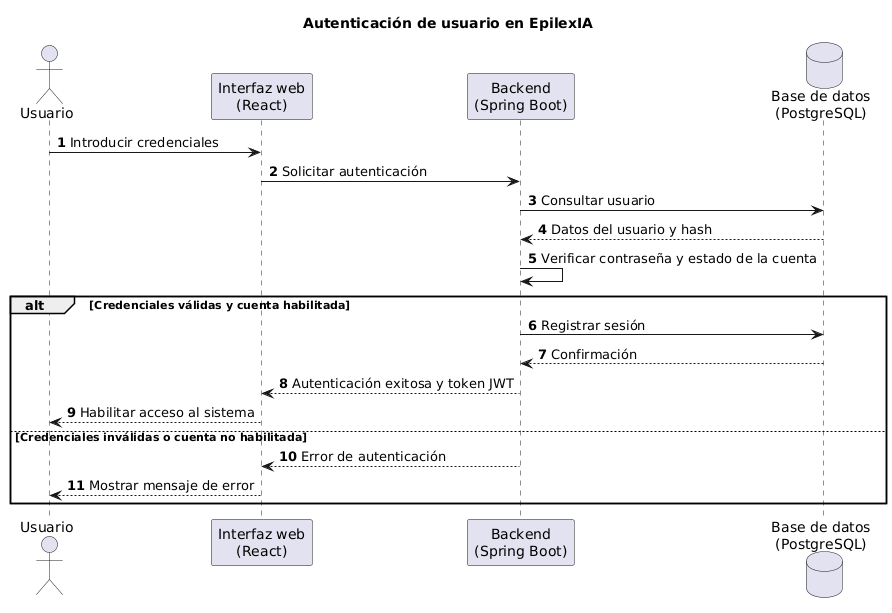
\includegraphics[width=0.95\textwidth]
    {ThesisFigs/secuencia_autenticacion.png}
    \caption{Diagrama de secuencia del proceso de
    autenticación de usuario en EpilexIA.}
    \label{fig:secuencia-autenticacion}
\end{figure}


\subsection{Registro y preparación de un estudio EEG}
\label{subsec:secuencia-registro-estudio}

El proceso de registro y preparación de un estudio EEG
comprende la identificación del paciente, la creación
del estudio y la incorporación de los archivos asociados.
Estas actividades se desarrollan en etapas diferenciadas,
que permiten gestionar el registro y el procesamiento
de las señales electroencefalográficas.

En la primera etapa, el usuario autorizado selecciona
un paciente existente o incorpora uno nuevo. Posteriormente,
completa la información del estudio, selecciona el archivo
EEG en formato EDF y, cuando corresponde, identifica
al Especialista responsable de su revisión. El \textit{backend}
verifica los datos y registra el estudio con estado inicial
Pendiente.

La Figura~\ref{fig:secuencia-registro-estudio} presenta
las principales interacciones de esta primera etapa.

\begin{figure}[H]
    \centering
    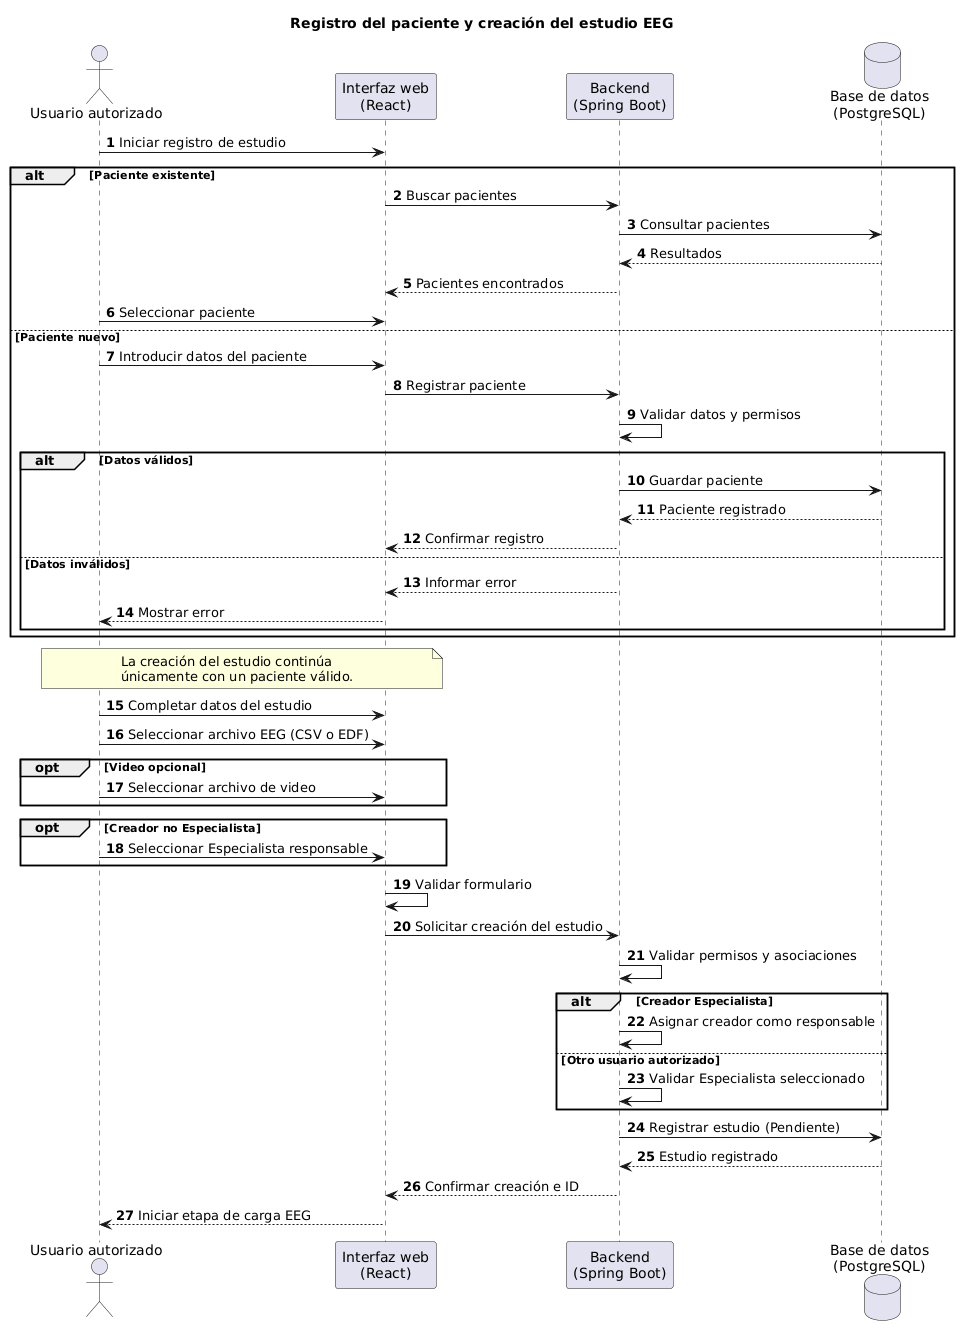
\includegraphics[
        width=\textwidth,
        height=0.82\textheight,
        keepaspectratio
    ]{ThesisFigs/secuencia_registro_estudio.png}
    \caption{Diagrama de secuencia del registro del paciente
    y creación del estudio EEG en EpilexIA.}
    \label{fig:secuencia-registro-estudio}
\end{figure}

Una vez registrado el estudio, el archivo EEG se transmite
al \textit{backend} mediante fragmentos. Al finalizar la carga,
se inicia el procesamiento correspondiente de manera
asíncrona. Durante esta etapa, la interfaz consulta
periódicamente el estado del estudio hasta obtener
un resultado de procesamiento exitoso o un error.

La Figura~\ref{fig:secuencia-preparacion-eeg} representa
la carga y preparación del archivo EEG, así como
el seguimiento de su estado.

\begin{figure}[H]
    \centering
    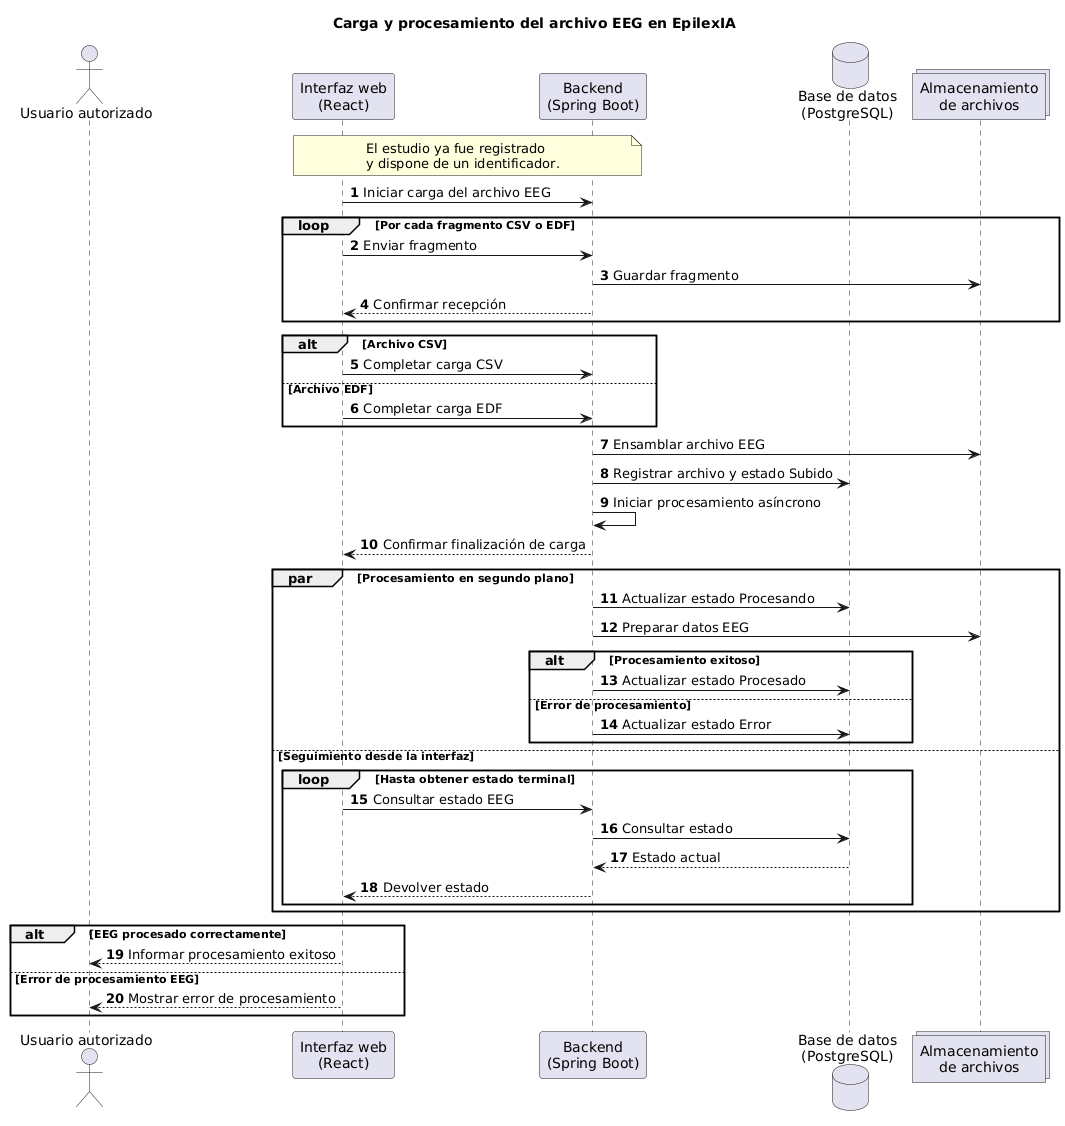
\includegraphics[
        width=\textwidth,
        height=0.82\textheight,
        keepaspectratio
    ]{ThesisFigs/secuencia_carga_procesamiento_eeg.png}
    \caption{Diagrama de secuencia de la carga y
    procesamiento del archivo EEG en EpilexIA.}
    \label{fig:secuencia-preparacion-eeg}
\end{figure}

Cuando el procesamiento del EEG finaliza correctamente,
el sistema permite continuar con la incorporación
de un video asociado, si corresponde. Los archivos
MP4 se gestionan mediante un procedimiento de carga
y almacenamiento, mientras que los archivos EZVideo,
formato de video propio del equipo Easy III,
requieren un proceso adicional de conversión a MP4.

La Figura~\ref{fig:secuencia-carga-video} muestra
las interacciones correspondientes a la carga y
preparación del video, incluyendo el seguimiento
de la conversión cuando se utiliza el formato EZVideo.

\begin{figure}[H]
    \centering
    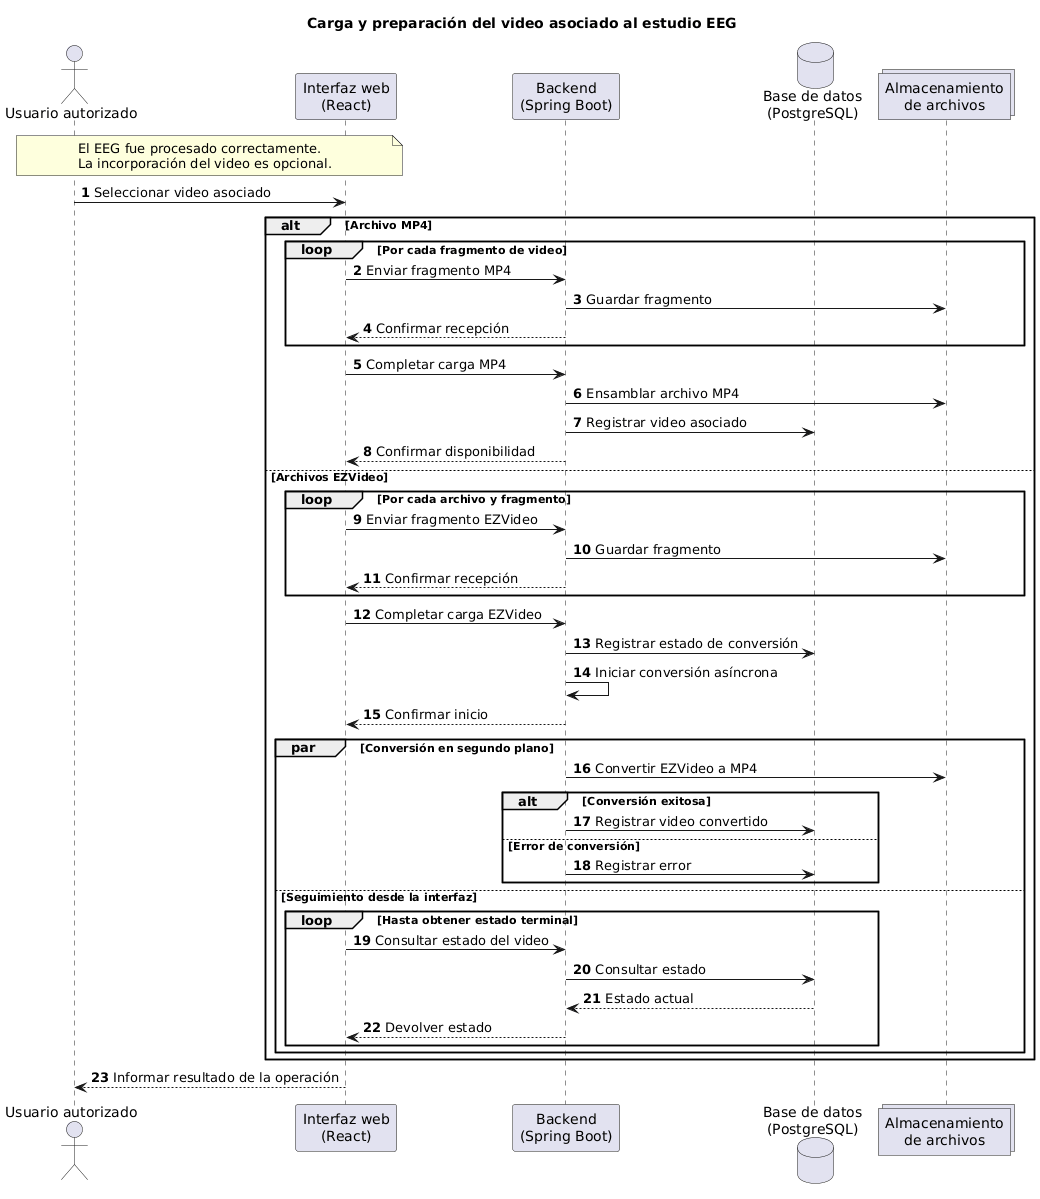
\includegraphics[
        width=\textwidth,
        height=0.82\textheight,
        keepaspectratio
    ]{ThesisFigs/secuencia_carga_video.png}
    \caption{Diagrama de secuencia de la carga y
    preparación del video asociado a un estudio EEG.}
    \label{fig:secuencia-carga-video}
\end{figure}


\subsection{Visualización de señales EEG}
\label{subsec:secuencia-visualizacion-eeg}

La visualización de señales EEG constituye una de las
funcionalidades principales de EpilexIA, ya que permite
al Especialista examinar los registros
electroencefalográficos asociados a un estudio.

El proceso comienza cuando el usuario autorizado accede
al visualizador. El sistema consulta la información del
estudio, verifica las condiciones de acceso y obtiene
los metadatos necesarios para presentar las señales.
Asimismo, recupera los montajes disponibles y establece
la configuración inicial de visualización.

Las señales EEG se obtienen mediante solicitudes de
segmentos correspondientes a intervalos temporales.
El \textit{backend} recupera los datos almacenados, aplica
los filtros configurados y organiza las derivaciones
según el montaje seleccionado. Posteriormente, la
interfaz web presenta las señales mediante una
representación gráfica multicanal.

La Figura~\ref{fig:secuencia-inicializacion-visualizador-eeg}
representa las principales interacciones correspondientes
al acceso al estudio, la recuperación de información y
la carga inicial de las señales EEG.

\begin{figure}[H]
    \centering
    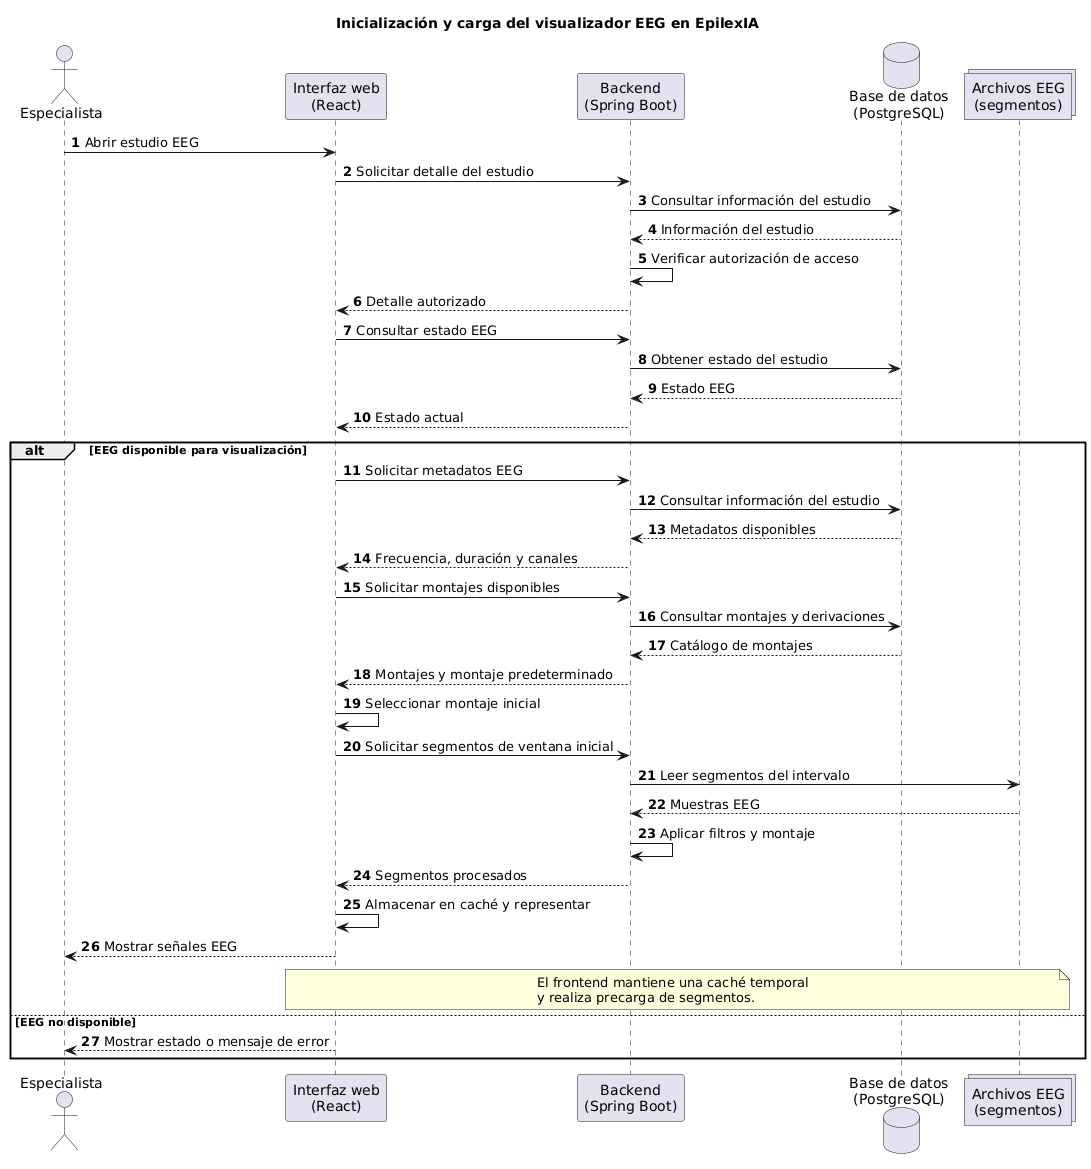
\includegraphics[
        width=\textwidth,
        height=0.82\textheight,
        keepaspectratio
    ]{ThesisFigs/secuencia_inicializacion_visualizador_eeg.png}
    \caption{Diagrama de secuencia de la inicialización
    y carga del visualizador EEG en EpilexIA.}
    \label{fig:secuencia-inicializacion-visualizador-eeg}
\end{figure}


Durante la revisión del estudio, el Especialista puede
desplazarse entre diferentes intervalos temporales,
seleccionar montajes y ajustar los filtros y la
sensibilidad de las señales. La navegación temporal
contempla dos modalidades complementarias: el
desplazamiento por segundos mediante los controles
de avance y retroceso, y el desplazamiento por ventanas
completas mediante las flechas horizontales del teclado.
La duración de cada ventana puede configurarse entre
5 y 25 segundos.

Asimismo, el Especialista puede modificar la
sensibilidad mediante las flechas verticales del
teclado, lo que permite ajustar la escala de
representación sin interrumpir la revisión del estudio.
Cuando existe un video asociado, la navegación
temporal mantiene la sincronización entre el cursor
EEG y la posición del video.

Para facilitar estas operaciones, el visualizador
mantiene temporalmente en memoria los segmentos
consultados y realiza una precarga de datos. Cuando
la información necesaria se encuentra disponible
en la caché, la representación gráfica puede
actualizarse sin realizar nuevas solicitudes al servidor.

El cambio de montaje o de filtros puede requerir
la recuperación y el procesamiento de nuevos segmentos
por parte del \textit{backend}. En cambio, el ajuste de
sensibilidad modifica la escala vertical de las señales
desde la interfaz web, sin necesidad de recuperar
nuevamente las muestras EEG. La sensibilidad
seleccionada puede conservarse como preferencia
del usuario.

La Figura~\ref{fig:secuencia-interacciones-visualizador-eeg}
presenta las interacciones correspondientes a la
navegación temporal, el cambio de montaje y los
ajustes de filtros y sensibilidad.

\begin{figure}[H]
    \centering
    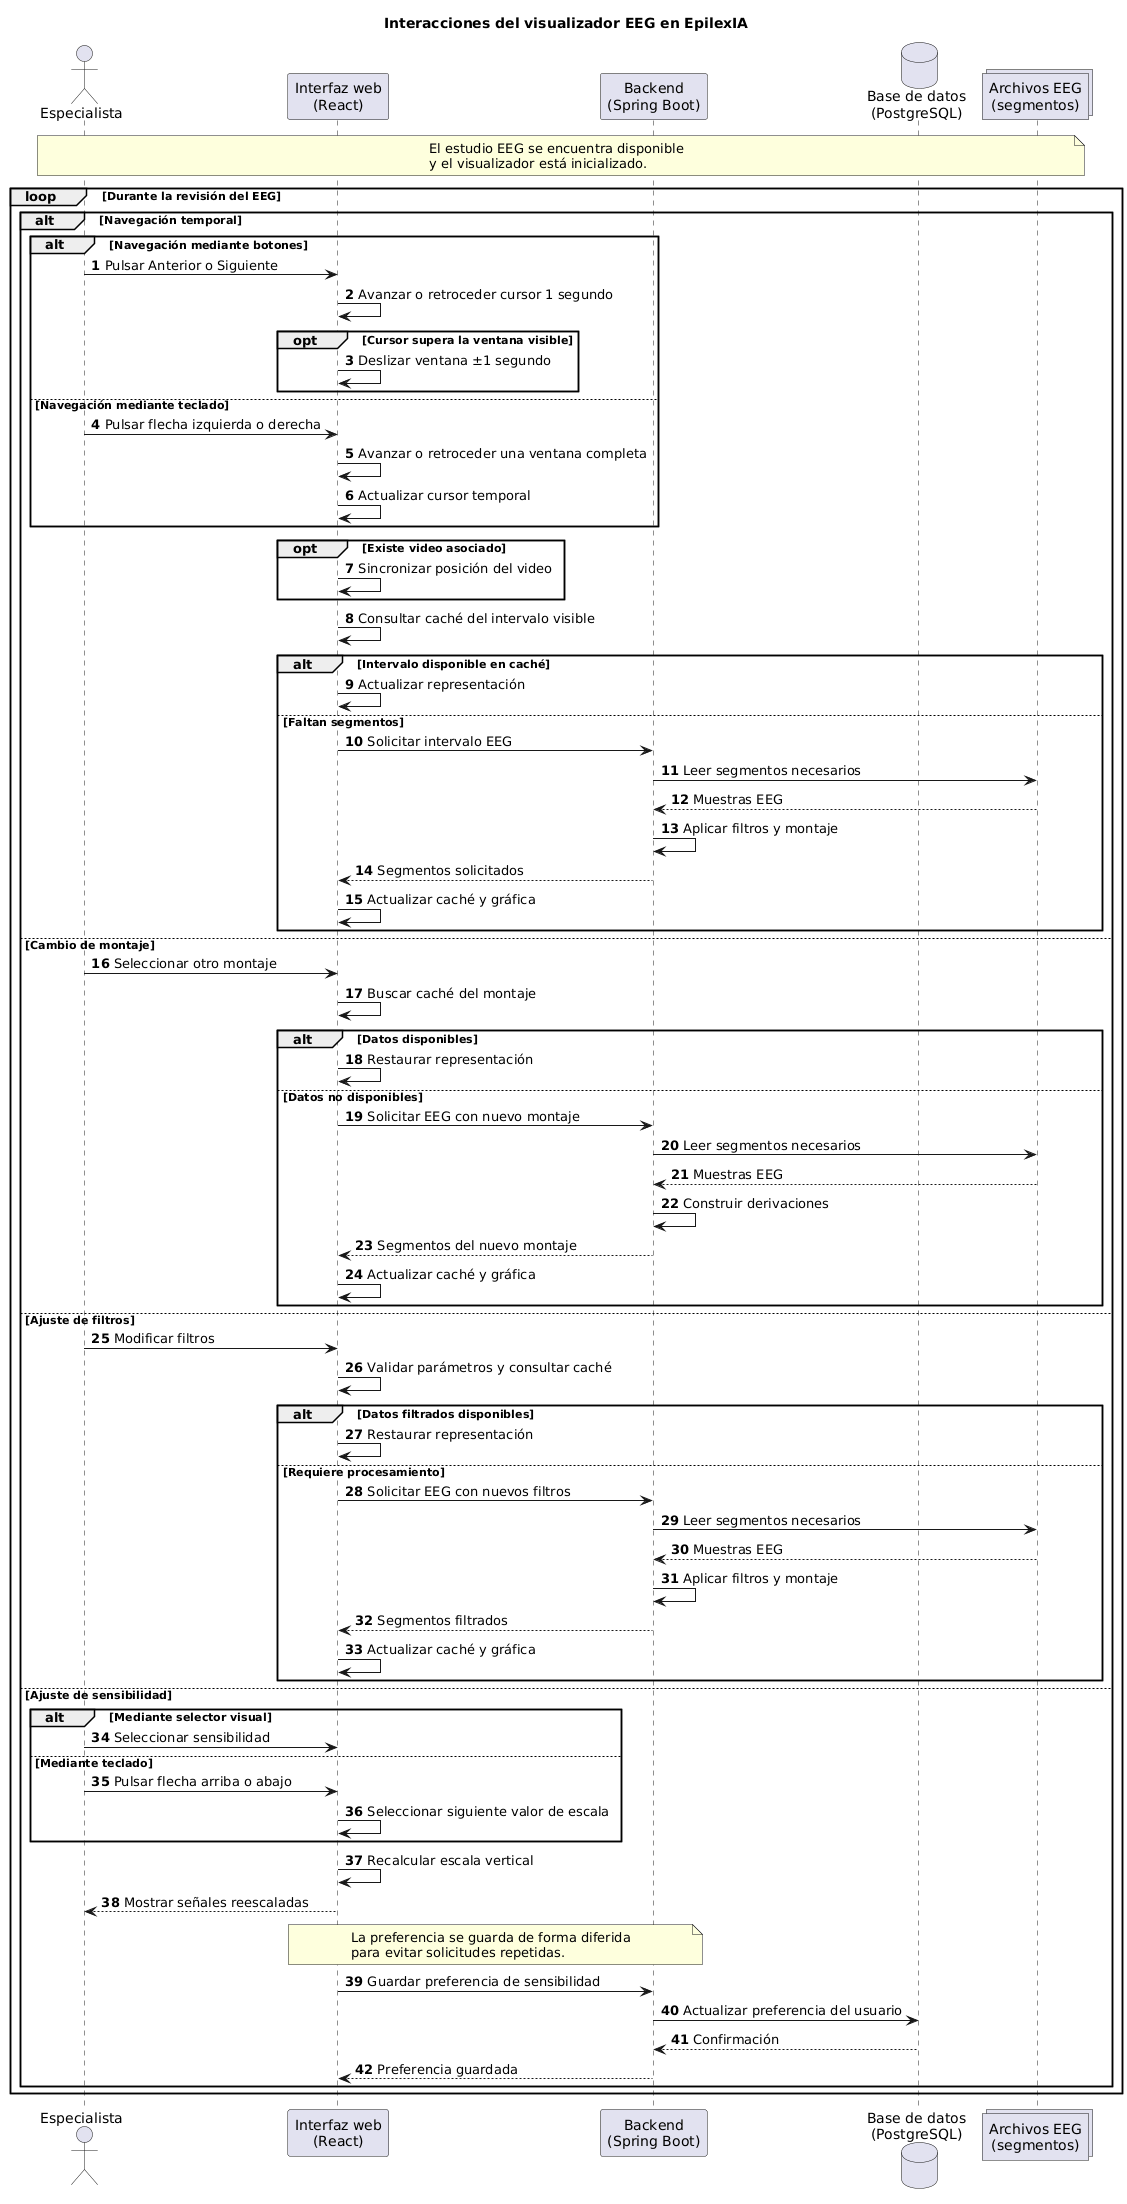
\includegraphics[
        width=\textwidth,
        height=0.82\textheight,
        keepaspectratio
    ]{ThesisFigs/secuencia_interacciones_visualizador_eeg.png}
    \caption{Diagrama de secuencia de las interacciones
    del visualizador EEG en EpilexIA.}
    \label{fig:secuencia-interacciones-visualizador-eeg}
\end{figure}


\subsection{Procesamiento de estudios mediante inteligencia artificial}
\label{subsec:secuencia-procesamiento-ia}

El procesamiento de estudios EEG mediante inteligencia
artificial constituye una funcionalidad de apoyo al
análisis realizado por el Especialista. Este proceso
permite solicitar el análisis automatizado de un
registro electroencefalográfico y consultar los
resultados obtenidos mediante el servicio de IA
integrado en EpilexIA.

La solicitud se origina en la interfaz web y es
recibida por el \textit{backend} clínico, que verifica
los permisos del usuario, las condiciones del
estudio y la disponibilidad del archivo EEG.
Cuando se cumplen las condiciones necesarias,
el \textit{backend} se comunica con la API de IA para
solicitar el procesamiento.

Antes de iniciar una nueva ejecución, el sistema
comprueba si existe una ejecución activa que pueda
ser reutilizada. Cuando corresponde iniciar un
nuevo procesamiento, la API de IA registra la
ejecución y devuelve su identificador y estado
inicial. El \textit{backend} conserva la referencia
correspondiente para permitir su seguimiento.

La Figura~\ref{fig:secuencia-solicitud-ia}
presenta las principales interacciones relacionadas
con la solicitud y el registro de una ejecución
de procesamiento mediante IA.

\begin{figure}[H]
    \centering
    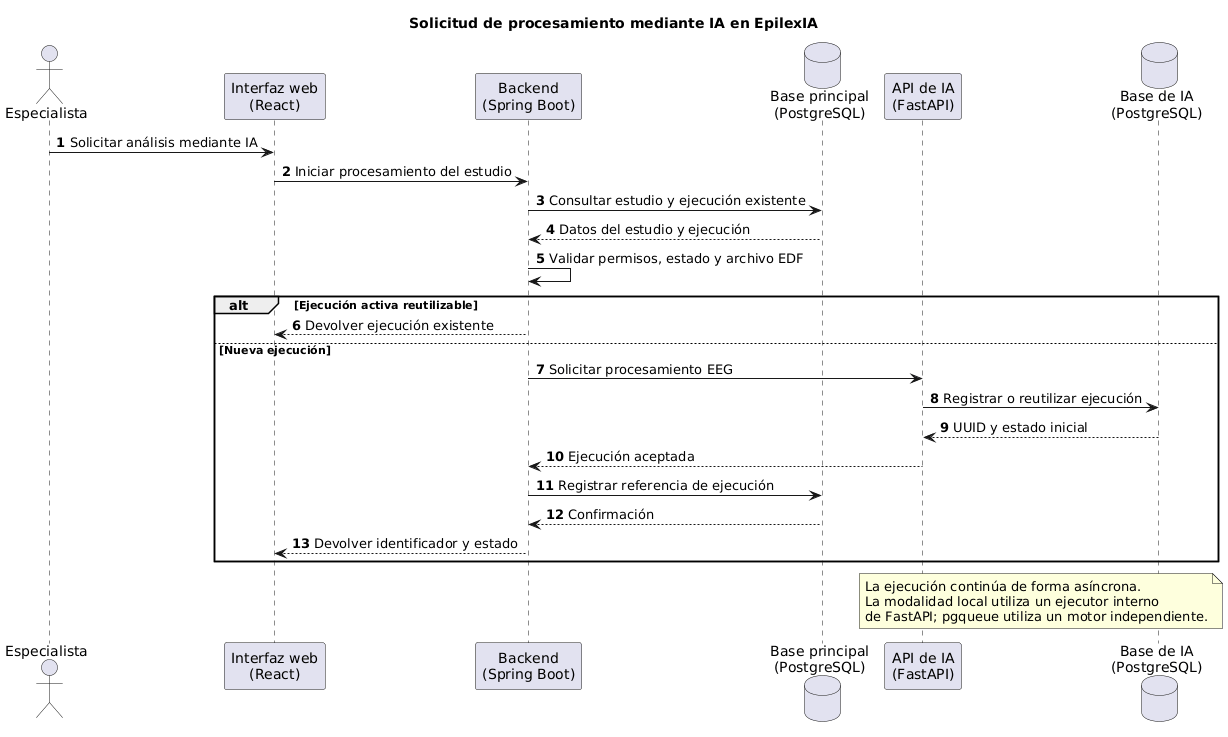
\includegraphics[
        width=\textwidth,
        height=0.82\textheight,
        keepaspectratio
    ]{ThesisFigs/secuencia_solicitud_ia.png}
    \caption{Diagrama de secuencia de la solicitud
    de procesamiento mediante inteligencia artificial
    en EpilexIA.}
    \label{fig:secuencia-solicitud-ia}
\end{figure}

El procesamiento se desarrolla de manera asíncrona,
por lo que la aceptación de una solicitud no implica
que el análisis haya finalizado. La ejecución se realiza a través de un motor independiente que obtiene
los trabajos desde una cola persistente.

Durante el procesamiento, la interfaz web consulta
periódicamente el estado de la ejecución. El \textit{backend}
obtiene la información correspondiente y, cuando
resulta necesario, consulta el estado actualizado
mediante la API de IA. Este mecanismo permite
identificar la finalización satisfactoria del
procesamiento o la ocurrencia de errores.

Una vez completada correctamente la ejecución,
el sistema permite recuperar los resultados
almacenados por el servicio de IA y presentarlos
al Especialista. Una ejecución exitosa puede
producir una lista vacía de anomalías, lo que
indica que no se registraron resultados que
cumplieran los criterios de detección establecidos
para dicha ejecución.

La Figura~\ref{fig:secuencia-resultados-ia}
representa el seguimiento del procesamiento
y la posterior consulta de los resultados
obtenidos mediante inteligencia artificial.

\begin{figure}[H]
    \centering
    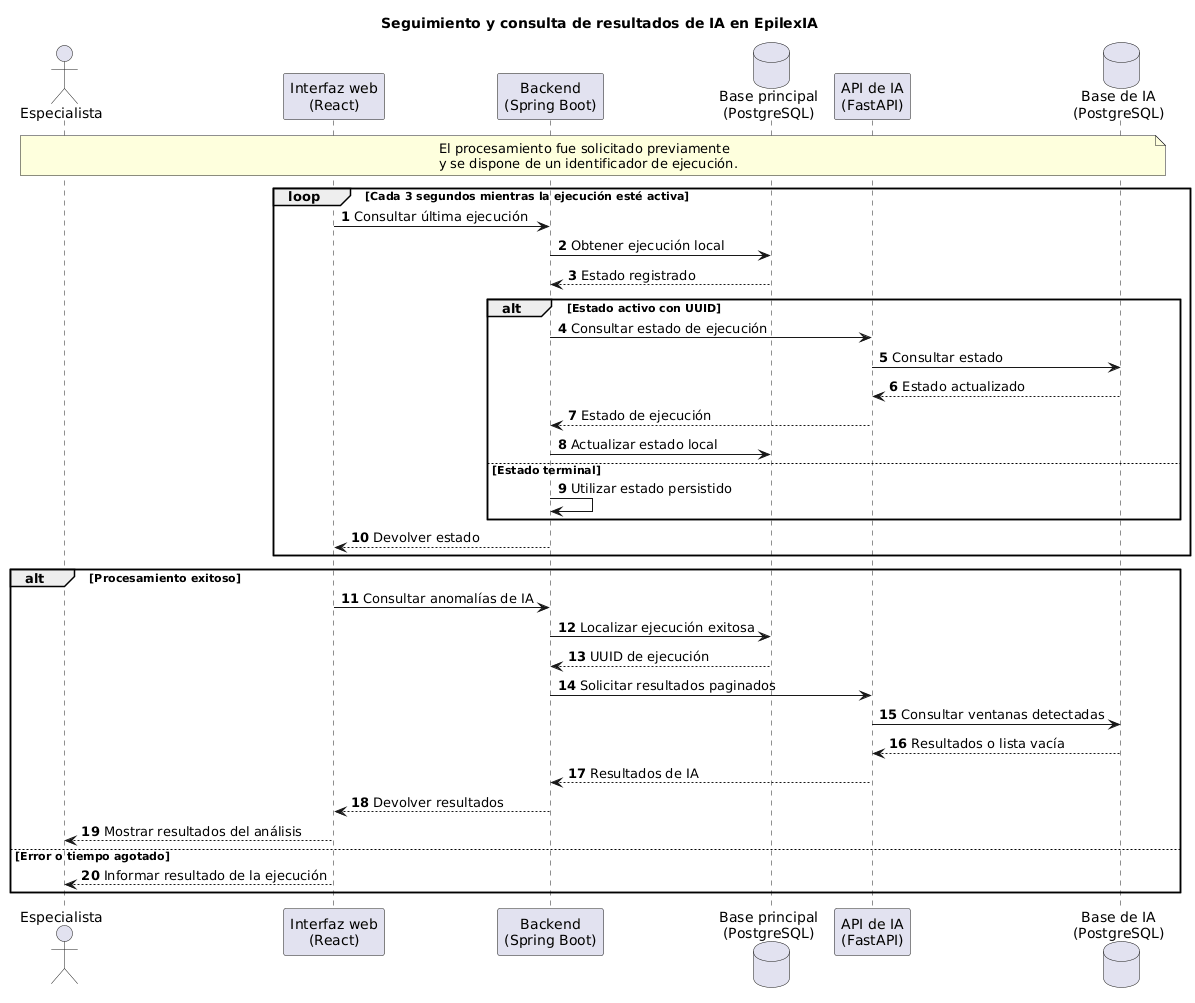
\includegraphics[
        width=\textwidth,
        height=0.82\textheight,
        keepaspectratio
    ]{ThesisFigs/secuencia_resultados_ia.png}
    \caption{Diagrama de secuencia del seguimiento
    y consulta de resultados de inteligencia
    artificial en EpilexIA.}
    \label{fig:secuencia-resultados-ia}
\end{figure}

Los resultados obtenidos mediante IA constituyen
información complementaria para la revisión
del estudio y se mantienen diferenciados de
las anotaciones manuales. Su interpretación
clínica corresponde al Especialista, por lo
que el procesamiento automatizado no sustituye
su criterio profesional.


\subsection{Elaboración y cierre de informes médicos}
\label{subsec:secuencia-informes-clinicos}

La elaboración de informes médicos constituye una
de las actividades principales realizadas por los
Especialistas durante la revisión de los estudios
electroencefalográficos. EpilexIA permite asociar
informes a un estudio EEG y mantener identificado
al profesional responsable de su elaboración.

El proceso comienza con la consulta de los informes
disponibles para el estudio. Un Especialista autorizado
puede acceder a los informes asociados y, cuando se
cumplen las condiciones correspondientes, crear
su propio informe. La creación genera un documento
en estado Borrador, inicialmente sin contenido clínico,
evitando que se reutilice información perteneciente
a informes elaborados por otros profesionales.

La Figura~\ref{fig:secuencia-creacion-informe}
presenta las interacciones involucradas en la
consulta y creación de informes médicos.

\begin{figure}[H]
    \centering
    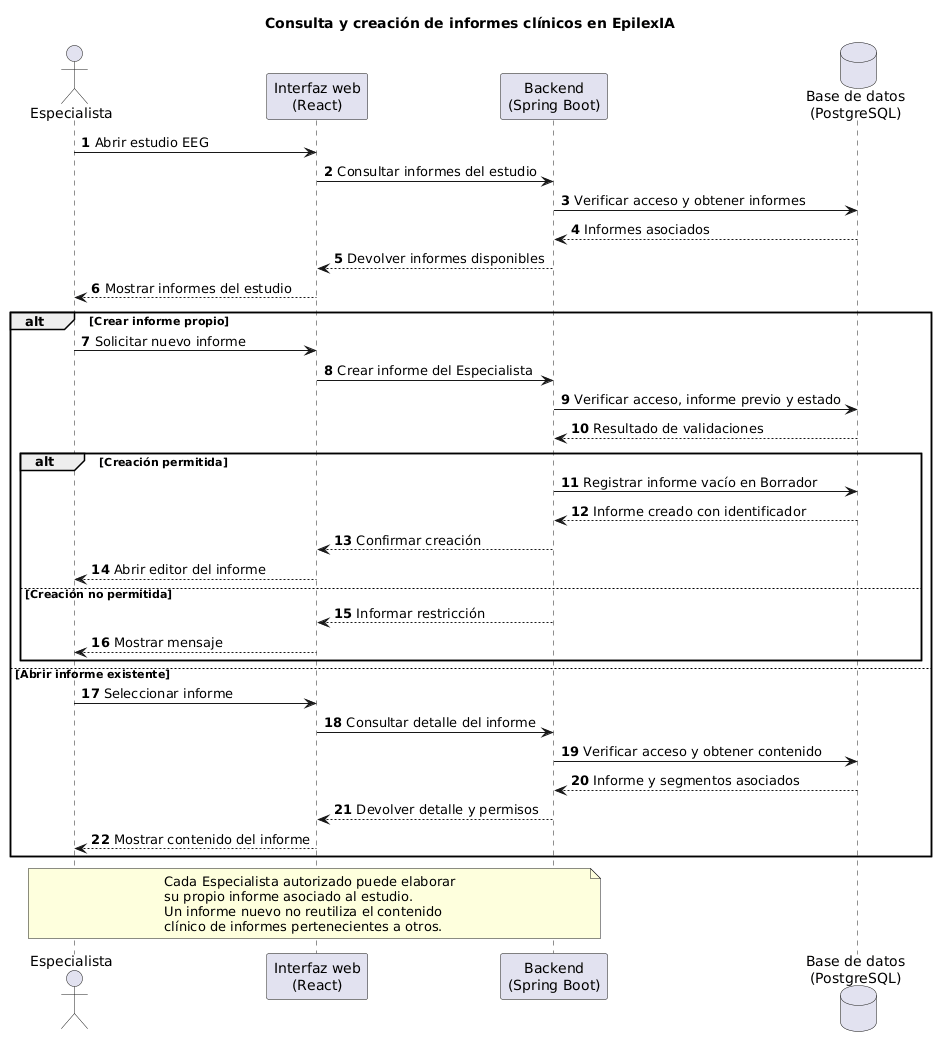
\includegraphics[
        width=\textwidth,
        height=0.82\textheight,
        keepaspectratio
    ]{ThesisFigs/secuencia_creacion_informe.png}
    \caption{Diagrama de secuencia de la consulta
    y creación de informes médicos en EpilexIA.}
    \label{fig:secuencia-creacion-informe}
\end{figure}

Durante la elaboración del informe, el Especialista
puede completar la información clínica correspondiente
e incorporar segmentos de interés identificados
durante la revisión del estudio EEG. Estos segmentos
pueden proceder de anotaciones manuales o de
resultados obtenidos mediante el procesamiento
por inteligencia artificial.

Las modificaciones realizadas se envían al \textit{backend},
donde se verifican las condiciones necesarias para
autorizar la actualización. Entre estas condiciones
se encuentran la identificación del propietario
del informe y su estado. De esta manera, el sistema
diferencia la edición del informe propio de la
consulta de documentos pertenecientes a otros
profesionales.

La Figura~\ref{fig:secuencia-edicion-informe}
representa las principales interacciones relacionadas
con la edición y actualización de informes médicos.

\begin{figure}[H]
    \centering
    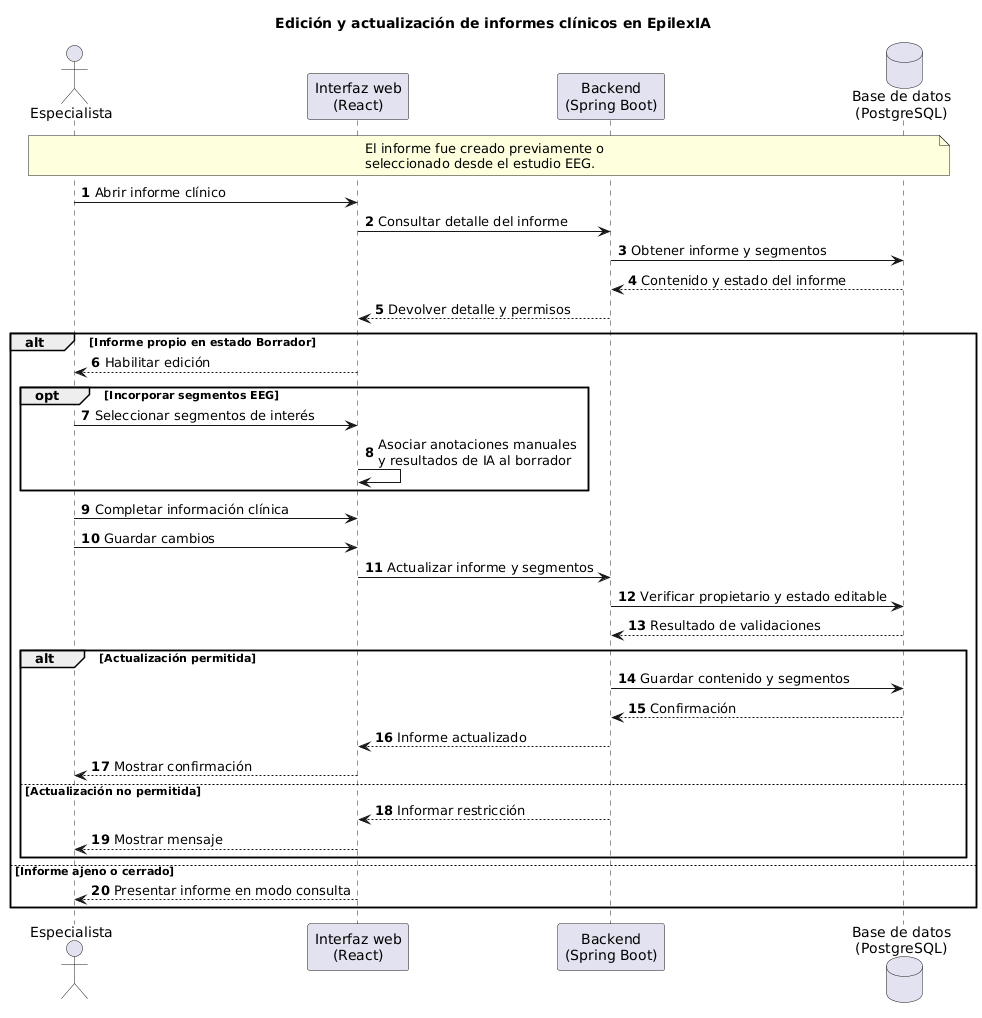
\includegraphics[
        width=\textwidth,
        height=0.82\textheight,
        keepaspectratio
    ]{ThesisFigs/secuencia_edicion_informe.png}
    \caption{Diagrama de secuencia de la edición
    y actualización de informes médicos en EpilexIA.}
    \label{fig:secuencia-edicion-informe}
\end{figure}

Una vez finalizada la elaboración del informe,
el Especialista responsable puede solicitar su cierre.
Esta operación requiere una validación específica,
diferente de la utilizada para guardar los cambios
durante la edición. Cuando se cumplen las condiciones establecidas, el sistema actualiza el informe al estado Cerrado y registra la fecha y hora correspondientes al cierre.

El cierre impide que el contenido clínico continúe
modificándose mediante el flujo ordinario de edición.
No obstante, el informe permanece disponible para
su consulta por parte de los usuarios autorizados.

Asimismo, EpilexIA permite generar una representación
del informe en formato PDF. Esta operación recupera
la información clínica y los segmentos asociados,
sin modificar el contenido del documento almacenado.

La Figura~\ref{fig:secuencia-cierre-informe}
presenta las interacciones correspondientes al
cierre y posterior consulta de informes médicos.

\begin{figure}[H]
    \centering
    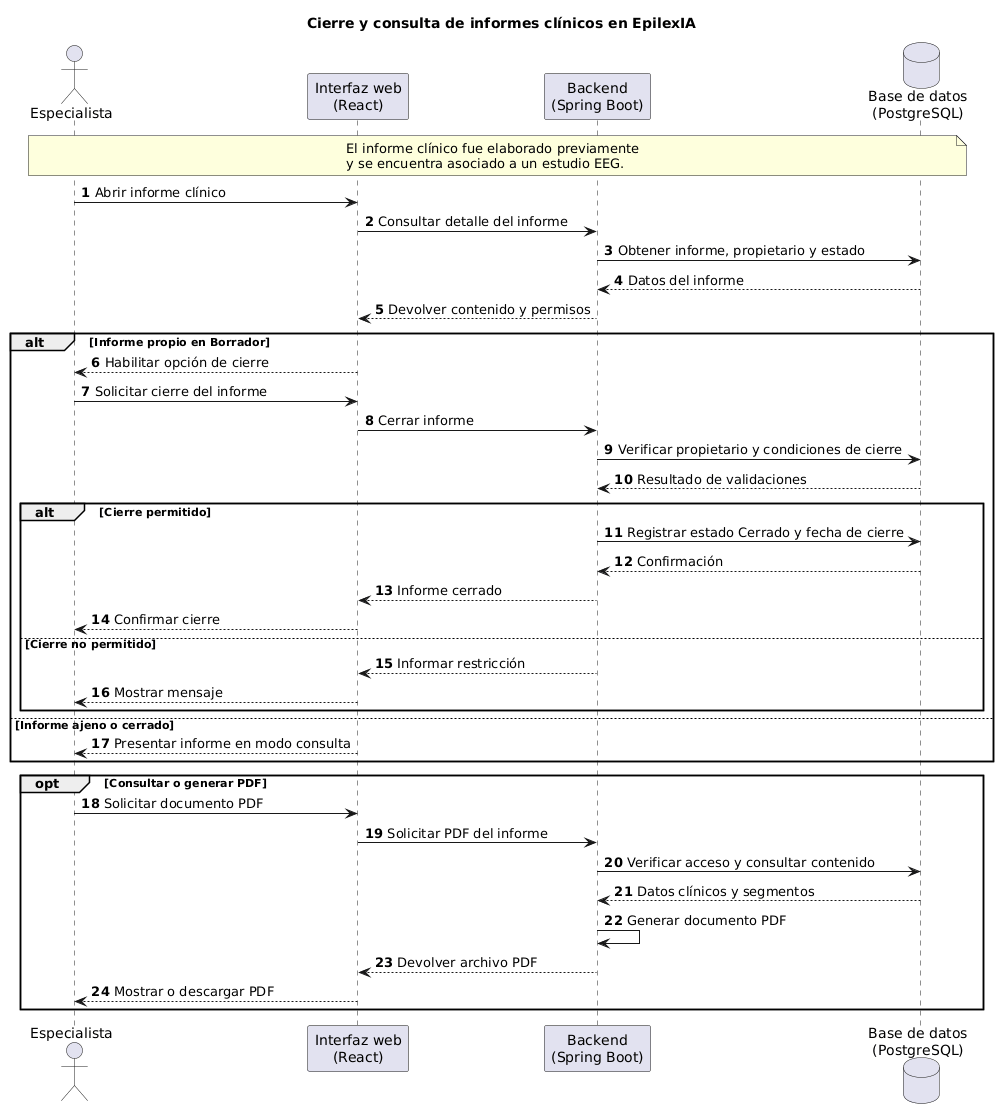
\includegraphics[
        width=\textwidth,
        height=0.82\textheight,
        keepaspectratio
    ]{ThesisFigs/secuencia_cierre_informe.png}
    \caption{Diagrama de secuencia del cierre
    y consulta de informes médicos en EpilexIA.}
    \label{fig:secuencia-cierre-informe}
\end{figure}

La separación entre creación, edición y cierre
permite conservar la identificación del profesional
responsable, controlar las modificaciones y mantener
la disponibilidad de los informes asociados a un
mismo estudio. Estas características contribuyen
a la organización del trabajo clínico y a la
trazabilidad de la información registrada.


\section{Arquitectura del sistema}
\label{sec:arquitectura-sistema}

La arquitectura de EpilexIA fue diseñada con el propósito de organizar
las funcionalidades del sistema en componentes diferenciados, de acuerdo
con sus responsabilidades dentro del proceso de gestión y análisis de
estudios electroencefalográficos.

La solución adopta una arquitectura web en la que se separan la
interfaz de usuario, la lógica de negocio, la persistencia de la
información y el procesamiento mediante inteligencia artificial.
Esta organización permite que los componentes se comuniquen mediante
interfaces definidas, manteniendo diferenciadas las operaciones
relacionadas con la gestión clínica y aquellas destinadas al
procesamiento automatizado de las señales EEG.

El diseño contempla la interacción entre los usuarios y la aplicación
web, la administración de la información asociada con pacientes y
estudios, el acceso a los archivos electroencefalográficos y la
integración de los resultados generados mediante inteligencia
artificial.

\subsection{Arquitectura general}
\label{subsec:arquitectura-general}

EpilexIA se organiza mediante una arquitectura cliente-servidor,
complementada con componentes especializados para el procesamiento
de señales EEG.

La interfaz web constituye el punto de acceso de los usuarios
autorizados. Desde ella se realizan las operaciones relacionadas
con la administración del sistema, la gestión de estudios, la
visualización de señales electroencefalográficas y la elaboración
de informes médicos.

Las solicitudes realizadas desde la interfaz son atendidas por
el \textit{backend} clínico, encargado de aplicar las reglas de negocio,
verificar las condiciones de acceso y coordinar las operaciones
necesarias para consultar o modificar la información almacenada.

La persistencia de la información estructurada se organiza mediante dos bases de datos PostgreSQL: una destinada a la gestión clínica y administrativa del sistema, y otra utilizada por el subsistema de inteligencia artificial para almacenar información relacionada con las ejecuciones y sus resultados. Por otra parte, los archivos asociados con los estudios EEG se conservan mediante mecanismos de almacenamiento independientes de las estructuras relacionales.

Para incorporar el análisis automatizado de las señales,
la arquitectura incluye un servicio de inteligencia artificial
integrado mediante una interfaz de programación de aplicaciones.
Este servicio permite gestionar las solicitudes de procesamiento
y consultar los resultados producidos por el componente de análisis.

La arquitectura también contempla la separación entre la
gestión de las ejecuciones de inteligencia artificial y el
procesamiento de las señales. De esta manera, las operaciones
de gestión clínica permanecen diferenciadas de las tareas
computacionales requeridas para el análisis automatizado.

%La Figura~\ref{fig:arquitectura-general} presenta la
%organización general de estos componentes y sus principales
%relaciones.
La Figura~\ref{fig:arquitectura-general} presenta la arquitectura general del sistema EpilexIA, organizada en componentes con responsabilidades diferenciadas. La capa de presentación proporciona la interfaz mediante la cual los usuarios autorizados interactúan con el sistema, mientras que la capa de aplicación concentra las reglas de negocio y coordina las operaciones relacionadas con la gestión de pacientes, estudios electroencefalográficos e informes médicos.

La persistencia principal comprende los repositorios destinados al almacenamiento de información clínica y administrativa, así como los archivos asociados a los estudios EEG y sus registros de video.

Por su parte, el subsistema de inteligencia artificial dispone de un servicio encargado de recibir y gestionar las solicitudes de análisis, administrar las ejecuciones y proporcionar acceso a los resultados obtenidos. Para la detección automática de crisis epilépticas, las tareas de análisis se registran en una cola persistente y son procesadas por un motor independiente.


En la configuración actualmente utilizada, el procesamiento destinado a la detección automática de crisis epilépticas se encuentra asignado al motor independiente. La coordinación entre este componente y el servicio de IA se establece mediante un repositorio compartido, diseñado para administrar las tareas pendientes, registrar los estados de ejecución y almacenar los resultados del análisis. Por otra parte, la arquitectura contempla la generación de espectrogramas DSA directamente en el servicio de IA, de forma independiente de la detección de crisis.


Esta organización establece una separación de responsabilidades entre los componentes del sistema y permite identificar los mecanismos de integración de la plataforma web con los servicios de inteligencia artificial, sin vincular la representación arquitectónica con tecnologías específicas de implementación. En este contexto, el presente trabajo de tesis se centra en el desarrollo de la plataforma web y en la integración del subsistema de inteligencia artificial, mientras que el desarrollo y el entrenamiento de los modelos de detección, a cargo del equipo de ciencia de datos, y la infraestructura tecnológica forman parte del proyecto integral EpilexIA.


\begin{figure}[H]
    \centering
    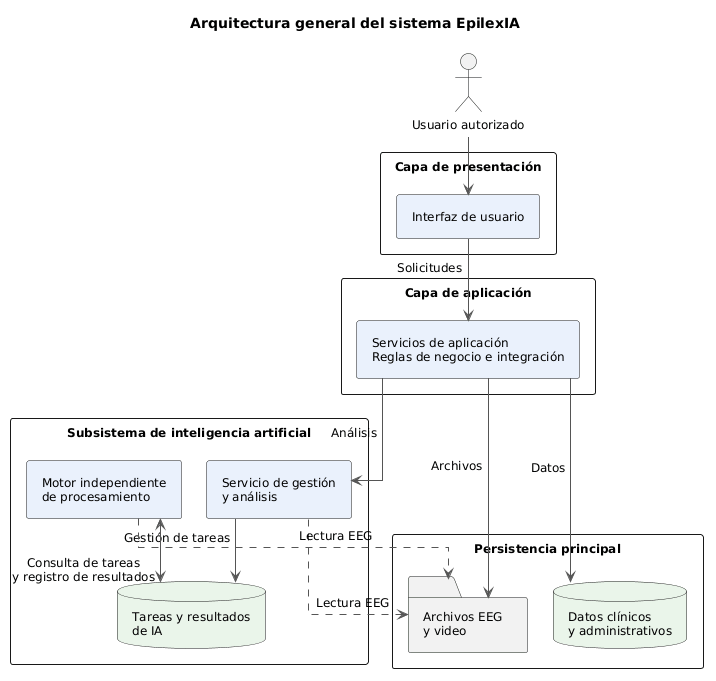
\includegraphics[width=\textwidth]{ThesisFigs/arquitectura_general_epilexia.png}
    \caption{Arquitectura general del sistema EpilexIA.}
    \label{fig:arquitectura-general}
\end{figure}


\subsection{Componentes de la arquitectura}
\label{subsec:componentes-arquitectura}

La arquitectura de EpilexIA está conformada por componentes
que cumplen responsabilidades específicas dentro del sistema.
Su organización permite separar las operaciones realizadas
por los usuarios, la gestión de la información clínica, el
almacenamiento de archivos y el procesamiento automatizado
de señales EEG.

Como se observa en la Figura~\ref{fig:arquitectura-general},
los componentes principales se distribuyen entre la capa
de presentación, la capa de aplicación, la persistencia
de datos y archivos, y el subsistema de inteligencia
artificial.

\subsubsection{Capa de presentación}

La capa de presentación corresponde a la interfaz web
desarrollada con React y TypeScript. Constituye el punto
de interacción entre los usuarios autorizados y las
funcionalidades disponibles en EpilexIA.

Este componente permite acceder a las operaciones de administración, gestionar la información de pacientes en el contexto de los estudios EEG, visualizar las señales electroencefalográficas, consultar los resultados del procesamiento mediante inteligencia artificial y elaborar informes médicos.

La interfaz organiza las funcionalidades disponibles de
acuerdo con los permisos del usuario autenticado y
se comunica con el \textit{backend} clínico mediante solicitudes
a una API REST.

\subsubsection{Capa de aplicación}

La capa de aplicación está representada por el \textit{backend} clínico, desarrollado en Java mediante Spring Boot y preparado para su despliegue como una aplicación WAR sobre el servidor de aplicaciones WildFly.

Este componente concentra las reglas de negocio
relacionadas con la gestión de usuarios, pacientes,
estudios EEG, informes médicos y eventos de auditoría.
Asimismo, verifica las condiciones de autorización
necesarias para ejecutar las operaciones solicitadas
desde la interfaz web.

El \textit{backend} también coordina el acceso a los datos
persistentes, la gestión de los archivos asociados
con los estudios y la comunicación con el servicio
de inteligencia artificial.

Esta organización permite mantener las validaciones
y las reglas de acceso en el servidor, independientemente
de los controles disponibles en la interfaz de usuario.

\subsubsection{Persistencia de datos y archivos}

La arquitectura contempla mecanismos diferenciados
para almacenar la información estructurada del sistema
y los archivos utilizados durante el análisis de los
estudios EEG.

La base de datos principal, implementada mediante
PostgreSQL, almacena la información correspondiente
a usuarios, pacientes, estudios, informes médicos,
permisos y registros de auditoría, así como las
relaciones necesarias entre estas entidades.

Por otra parte, los archivos asociados con los
estudios, como los registros electroencefalográficos
y los videos, se conservan mediante mecanismos
de almacenamiento de archivos.

Esta separación permite que la base de datos
mantenga las referencias y los metadatos necesarios
para relacionar los archivos con los estudios,
sin incorporar directamente su contenido completo
a las estructuras relacionales.

\subsubsection{Subsistema de inteligencia artificial}

El subsistema de inteligencia artificial constituye
un conjunto de componentes especializados que
permiten incorporar el procesamiento automatizado
de señales EEG al funcionamiento de EpilexIA.


La comunicación con este subsistema se realiza mediante una API desarrollada con FastAPI, que recibe las solicitudes provenientes del \textit{backend} clínico y proporciona los mecanismos necesarios para consultar el estado de las ejecuciones y recuperar los resultados almacenados. La arquitectura contempla, además, la ejecución de nuevas tareas de procesamiento mediante los componentes especializados del subsistema.


El subsistema dispone de una base de datos
PostgreSQL destinada a gestionar la información
relacionada con las ejecuciones de procesamiento
y sus resultados.

Las solicitudes pendientes se gestionan mediante una cola persistente en la base de datos de IA, denominada \texttt{pgqueue}, y son atendidas por un motor de procesamiento independiente.


La arquitectura tiene como propósito facilitar la recuperación y consulta de los resultados obtenidos mediante inteligencia artificial, de manera que puedan utilizarse como información complementaria durante la revisión de los estudios EEG.  La verificación del ciclo completo, desde la solicitud del análisis hasta la presentación de nuevos resultados, se documenta en el Anexo~\ref{pruebas_evaluacion}.


El desarrollo y entrenamiento del modelo de
inteligencia artificial no forman parte del alcance
de este trabajo, cuya participación
se concentra en su integración con los componentes
del sistema y en la presentación de los resultados
para su revisión por parte del Especialista.


\subsection{Comunicación entre componentes}
\label{subsec:comunicacion-componentes}

La comunicación entre los componentes de EpilexIA se
organiza a partir de las solicitudes realizadas por
los usuarios mediante la interfaz web. Estas solicitudes
son atendidas por el \textit{backend} clínico, que coordina
las operaciones necesarias y establece la comunicación
con los mecanismos de persistencia y los servicios
especializados del sistema.

La interacción entre la capa de presentación y la
capa de aplicación se realiza mediante una API REST.
A través de esta interfaz, el \textit{frontend} envía las
solicitudes relacionadas con la autenticación,
la gestión de pacientes y estudios EEG, la consulta
de señales electroencefalográficas y la elaboración
de informes médicos.

El \textit{backend} recibe estas solicitudes, verifica las
condiciones de acceso correspondientes y ejecuta
las reglas de negocio asociadas con cada operación.
Posteriormente, devuelve las respuestas necesarias
para que la interfaz actualice la información
presentada al usuario.

Para las operaciones que requieren información
persistente, el \textit{backend} interactúa con la base
de datos principal PostgreSQL. Esta comunicación
permite consultar y actualizar los registros
relacionados con usuarios, pacientes, estudios,
informes y eventos de auditoría.

En el caso de los archivos asociados con los
estudios EEG, el \textit{backend} coordina las operaciones
de almacenamiento y recuperación de los datos
necesarios para su posterior procesamiento
y visualización. La información estructurada
que identifica y relaciona estos archivos
con los estudios se conserva en la base de
datos principal.

La comunicación con el subsistema de inteligencia
artificial se establece mediante la API desarrollada
con FastAPI. Cuando se solicita el procesamiento
automatizado de un estudio, el \textit{backend} clínico
verifica las condiciones necesarias y transmite
la solicitud al servicio de IA.


La arquitectura contempla el procesamiento asíncrono de las solicitudes de análisis, de manera que la operación inicial no requiera mantener al usuario esperando hasta la finalización del procesamiento. Para ello, se dispone de mecanismos destinados a consultar el estado de las ejecuciones y recuperar los resultados almacenados cuando estén disponibles.


Dentro del subsistema de IA, las ejecuciones pendientes son atendidas por un motor independiente
que utiliza la base de datos de IA para gestionar
los trabajos y registrar sus resultados.


Los resultados de inteligencia artificial almacenados pueden recuperarse mediante la comunicación entre el \textit{backend} clínico y la API de IA. Posteriormente, la interfaz web permite presentarlos en el contexto del estudio correspondiente, de manera que el Especialista pueda examinarlos junto con las señales EEG. Este mecanismo contempla tanto la consulta de resultados existentes como la recuperación de nuevos resultados cuando finalicen las ejecuciones de procesamiento.


Esta organización permite mantener una
comunicación diferenciada entre los componentes
encargados de la gestión del sistema y aquellos
destinados al procesamiento automatizado,
conservando al \textit{backend} clínico como punto
de coordinación de las operaciones solicitadas
desde la interfaz web.


\section{Diseño de la base de datos}
\label{sec:diseno-base-datos}

El diseño de persistencia de EpilexIA contempla
la separación de la información clínica y operativa
del sistema respecto de los datos utilizados para
coordinar el procesamiento mediante inteligencia
artificial. Para ello, se emplean dos bases de datos
relacionales PostgreSQL, con responsabilidades
diferenciadas.

\subsection{Organización general de los datos}
\label{subsec:organizacion-datos}

La base de datos principal almacena la información
estructurada necesaria para la gestión de usuarios,
pacientes, estudios EEG, informes médicos, anomalías
registradas y demás operaciones de la plataforma.
Esta información permite establecer las relaciones
entre los estudios y los profesionales que intervienen
en su registro, revisión e interpretación.

Por otra parte, el subsistema de inteligencia artificial
dispone de una base de datos independiente, destinada
a gestionar las solicitudes de procesamiento, sus
estados de ejecución y los resultados obtenidos.
Esta base de datos permite coordinar las actividades
entre la API de inteligencia artificial y el motor
de procesamiento.

Los archivos que contienen las señales EEG y los
videos asociados se conservan en un almacenamiento
de archivos independiente de las tablas relacionales.
De esta manera, la información estructurada del
sistema puede relacionarse con los registros
electroencefalográficos sin requerir que el contenido
completo de dichos archivos se almacene directamente
en la base de datos clínica.


\subsection{Modelo de datos clínicos}
\label{subsec:modelo-datos-clinicos}

El modelo de datos clínicos de EpilexIA se estructura
principalmente alrededor de las entidades
\texttt{patient} y \texttt{study}, que representan,
respectivamente, a los pacientes registrados y sus
estudios electroencefalográficos. La relación entre
ambas entidades es de uno a muchos, dado que un
paciente puede tener varios estudios EEG, mientras
que cada estudio corresponde a un único paciente.

La entidad \texttt{study} constituye el núcleo del modelo y mantiene referencias a los usuarios que intervienen en la gestión del estudio. Cada estudio debe estar asociado obligatoriamente a un usuario responsable, cuya pertenencia al perfil Especialista se verifica mediante las reglas de negocio del \textit{backend} durante su creación. Asimismo, puede incluir de manera opcional un técnico encargado de su registro. La entidad también conserva información sobre el estado del estudio, su anulación, reactivación y disponibilidad de video.

Los archivos asociados a cada estudio se representan mediante la entidad
\texttt{study\_file}, relacionada con el catálogo
\texttt{study\_file\_type}, que permite identificar el formato
correspondiente. Esta estructura admite múltiples archivos por estudio,
incluyendo señales EEG y videos, y conserva metadatos técnicos como la
duración, la frecuencia de muestreo y los canales disponibles.
Estos metadatos se registran o completan durante las operaciones de carga
y procesamiento de los archivos, de acuerdo con las características y
los mecanismos de lectura de cada formato.

Para representar las configuraciones de visualización,
el modelo incorpora las entidades \texttt{eeg\_montage}
y \texttt{eeg\_montage\_channel}. La primera define los
montajes electroencefalográficos disponibles, mientras
que la segunda establece los canales o derivaciones
que componen cada montaje y su orden de presentación.

Los hallazgos registrados durante la revisión de un
estudio se organizan en dos estructuras diferenciadas.
La entidad \texttt{anomaly} representa intervalos de
señal identificados manualmente o mediante inteligencia
artificial, con referencias opcionales a su clasificación
y montaje. Por otra parte, \texttt{study\_eeg\_event}
almacena eventos temporales asociados al estudio,
utilizando tipos predefinidos o personalizados.


La elaboración de informes médicos se modela mediante las entidades \texttt{report}, \texttt{study\_report} y \texttt{report\_segment}. La entidad \texttt{report} almacena el contenido clínico del informe, mientras que \texttt{study\_report} establece la asociación entre el estudio, el Especialista y el informe correspondiente. Esta relación permite la existencia de informes elaborados por diferentes Especialistas para un mismo estudio, con la restricción de un único informe por Especialista dentro de dicho estudio.


Finalmente, \texttt{report\_segment} permite asociar
a cada informe los intervalos de señal considerados
relevantes, conservando información sobre su ubicación
temporal y, cuando corresponde, sus referencias a
anomalías, montajes o ejecuciones de inteligencia
artificial.

El modelo se complementa con estructuras de control
de acceso, compartición de estudios y auditoría,
que permiten relacionar las operaciones clínicas con
los usuarios participantes y conservar información
para su trazabilidad.


La Figura~\ref{fig:er-pacientes-estudios}
presenta las principales entidades relacionadas
con el registro de pacientes, la gestión de estudios
electroencefalográficos, sus archivos asociados
y las configuraciones de montaje EEG.

Por su parte, la Figura~\ref{fig:er-informes-anomalias}
representa las relaciones entre los estudios,
las anomalías, los eventos EEG y los informes
médicos elaborados por los especialistas.
Ambas figuras constituyen vistas simplificadas
del modelo relacional, en las que se priorizan
las entidades y asociaciones más relevantes
para comprender el diseño del sistema.


\begin{figure}[H]
    \centering
    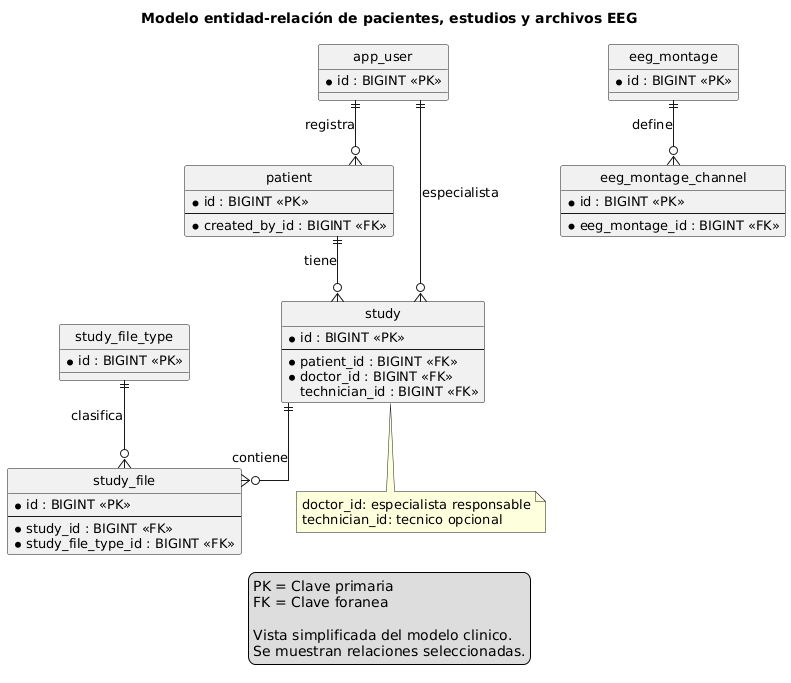
\includegraphics[width=\textwidth]{ThesisFigs/er_pacientes_estudios.png}
    \caption{Modelo entidad-relación de pacientes,
    estudios y archivos EEG de EpilexIA.}
    \label{fig:er-pacientes-estudios}
\end{figure}

\begin{figure}[H]
    \centering
    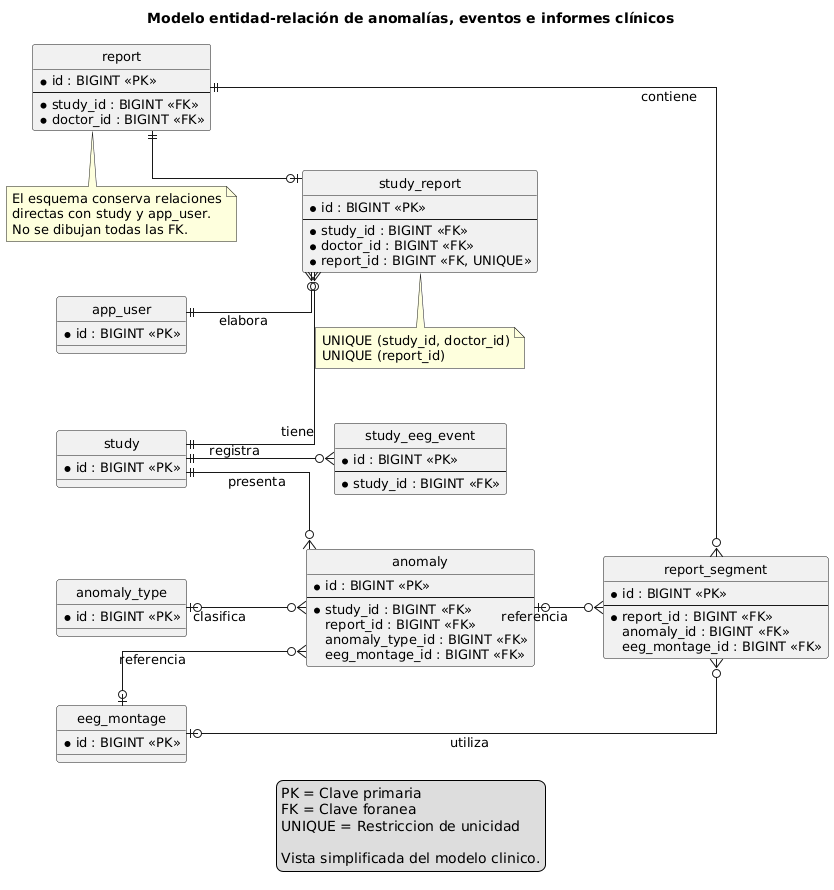
\includegraphics[width=\textwidth]{ThesisFigs/er_informes_anomalias.png}
    \caption{Modelo entidad-relación de anomalías,
    eventos e informes médicos de EpilexIA.}
    \label{fig:er-informes-anomalias}
\end{figure}


\subsection{Modelo de datos del procesamiento de inteligencia artificial}
\label{subsec:modelo-datos-ia}

El subsistema de inteligencia artificial de EpilexIA utiliza una base de datos PostgreSQL independiente de la base de datos clínica principal. Su diseño permite registrar las solicitudes de procesamiento de señales EEG, controlar los estados de ejecución, almacenar los resultados obtenidos y conservar información de retroalimentación proporcionada por los especialistas. El esquema comprende seis tablas principales, cuya estructura es administrada mediante migraciones de la API de inteligencia artificial desarrollada con FastAPI.

La entidad central del modelo es \texttt{ai\_executions}, que representa cada solicitud de análisis electroencefalográfico. Cada ejecución se identifica mediante un UUID y conserva información sobre el estudio asociado, el modelo utilizado, su versión, el umbral mínimo de probabilidad y la ubicación del archivo EEG que debe procesarse. Asimismo, registra el estado de ejecución, las fechas de inicio y finalización y los datos operativos necesarios para identificar posibles errores.

El ciclo de vida de una ejecución se representa mediante estados como \texttt{QUEUED}, \texttt{RUNNING}, \texttt{SUCCESS}, \texttt{FAILED}, \texttt{TIMEOUT} y \texttt{CANCELLED}. Adicionalmente, el subsistema contempla el estado interno \texttt{CANCEL\_REQUESTED}, utilizado para coordinar las solicitudes de cancelación durante el procesamiento mediante cola.

La configuración del modelo activo se administra mediante la entidad \texttt{ai\_model\_params}, que almacena parámetros como el nombre, la versión y el umbral mínimo de probabilidad de crisis. Al registrar una ejecución, estos valores se incorporan a \texttt{ai\_executions}, permitiendo conservar la configuración utilizada en cada procesamiento. Los archivos que contienen los modelos entrenados se mantienen fuera de la base de datos, en un almacenamiento independiente.

Los resultados del análisis se representan mediante la entidad \texttt{ai\_results}, relacionada con \texttt{ai\_executions} mediante una clave foránea. Cada registro corresponde a un intervalo temporal identificado por el procesamiento de inteligencia artificial y conserva su instante inicial, instante final y probabilidad estimada de crisis. El sistema almacena únicamente las ventanas clasificadas positivamente que cumplen el umbral mínimo configurado. Por consiguiente, una ejecución finalizada correctamente puede no generar registros de resultados cuando no se identifican intervalos que satisfagan dicho criterio.

El modelo incorpora mecanismos para conservar la revisión realizada por los especialistas. La entidad \texttt{ai\_results} dispone de atributos destinados a registrar la validación médica de los intervalos detectados. Por su parte, \texttt{ai\_report\_window\_inclusions} permite asociar los resultados de inteligencia artificial con los informes médicos en los que fueron incluidos, conservando información descriptiva y de clasificación aportada por el profesional.

Complementariamente, la entidad \texttt{ai\_manual\_annotations} almacena anotaciones realizadas manualmente por los especialistas, incluso cuando no corresponden a intervalos detectados previamente por el modelo. Estas estructuras permiten conservar información de retroalimentación clínica que podría utilizarse en futuros procesos de mejora de los modelos de inteligencia artificial, sin que ello implique la existencia de un mecanismo automático de reentrenamiento en la implementación actual.

La base de datos también contempla la entidad \texttt{ai\_results\_historial}, destinada al almacenamiento histórico de resultados. Esta estructura se encuentra definida en el esquema; el traslado automático de registros hacia ella desde la tabla de resultados activos no está implementado en la versión actual.

La tabla \texttt{ai\_executions} cumple además una función de coordinación entre la API de inteligencia artificial y el motor de procesamiento independiente. La API registra las solicitudes pendientes y el motor adquiere los trabajos mediante operaciones transaccionales sobre PostgreSQL. Durante la ejecución se actualizan los estados y las señales de actividad del procesamiento, mientras que al finalizar se registran los resultados y el estado correspondiente.

La vinculación con la base de datos clínica se establece mediante identificadores compartidos a nivel de aplicación. En particular, \texttt{id\_study\_epilex} permite identificar el estudio clínico asociado, mientras que el UUID de la ejecución puede relacionarse con los registros de seguimiento mantenidos por el \textit{backend} clínico. Debido a que ambas bases de datos funcionan de manera independiente, estas correspondencias no se implementan mediante claves foráneas entre ellas.

Finalmente, los archivos EEG, los modelos entrenados y los archivos temporales generados durante el procesamiento se conservan en almacenamiento de archivos. Esta separación permite mantener en PostgreSQL los datos estructurados necesarios para la gestión, consulta y trazabilidad de las ejecuciones, sin incorporar directamente los archivos de señales ni los artefactos del modelo.


La Figura~\ref{fig:er-subsistema-ia} presenta
una vista simplificada del modelo entidad-relación
del subsistema de inteligencia artificial de EpilexIA.
Se destacan las relaciones entre las ejecuciones
de procesamiento, los resultados generados y las
ventanas incorporadas a informes médicos.
Asimismo, se representan las estructuras destinadas
a la configuración del modelo, las anotaciones
manuales y el almacenamiento histórico, diferenciando
las relaciones definidas mediante claves foráneas
de las referencias lógicas gestionadas por la aplicación.


\begin{figure}[H]
    \centering
    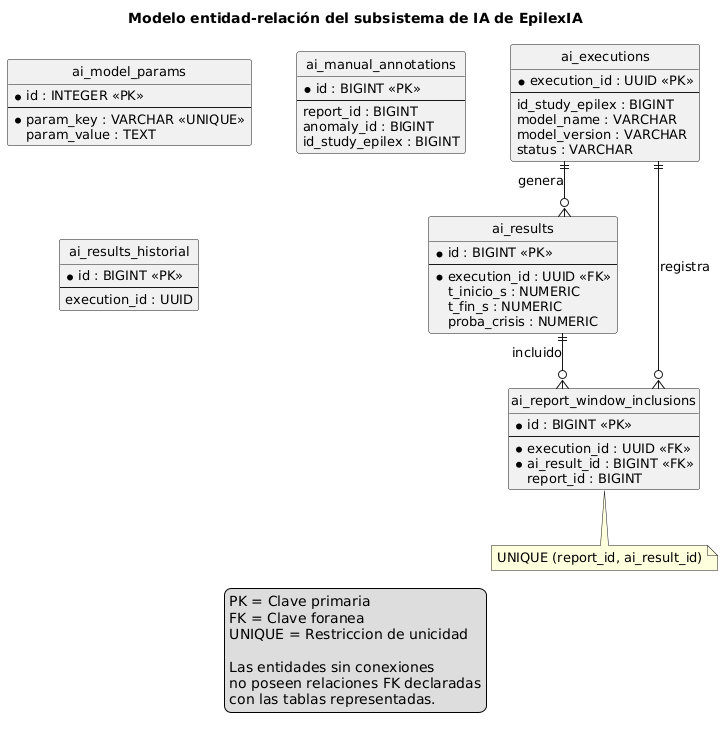
\includegraphics[width=\textwidth]{ThesisFigs/er_subsistema_ia.png}
    \caption{Modelo entidad-relación del subsistema
    de inteligencia artificial de EpilexIA.}
    \label{fig:er-subsistema-ia}
\end{figure}


\subsection{Integridad y persistencia de los datos}
\label{subsec:integridad-persistencia-datos}

El diseño de persistencia de EpilexIA contempla mecanismos
de integridad orientados a mantener la consistencia de
la información clínica y de los registros asociados al
procesamiento mediante inteligencia artificial. Para ello,
las bases de datos PostgreSQL emplean claves primarias,
claves foráneas y restricciones de unicidad que permiten
identificar los registros y controlar sus relaciones.

En la base de datos clínica, las restricciones de integridad
referencial permiten establecer asociaciones entre pacientes,
estudios electroencefalográficos, archivos, anomalías e
informes médicos. Estas relaciones contribuyen a evitar
referencias a registros inexistentes y a mantener la
correspondencia entre los estudios y la información generada
durante su revisión. Asimismo, determinadas restricciones
de unicidad permiten aplicar reglas del modelo, como la
existencia de un único informe por Especialista dentro
de un mismo estudio.

En la base de datos del subsistema de inteligencia artificial,
la integridad referencial se aplica principalmente a las
relaciones entre las ejecuciones de procesamiento, los
resultados obtenidos y los registros de inclusión de ventanas
en informes médicos. Cada resultado se vincula con la
ejecución que lo generó, permitiendo identificar su origen
y conservar la trazabilidad de los intervalos detectados
por el modelo.

La separación entre la base de datos clínica y la base
de datos de inteligencia artificial implica que sus
correspondencias se gestionan mediante identificadores
compartidos a nivel de aplicación, sin establecer claves
foráneas entre ambas bases. De esta manera, cada subsistema
mantiene sus propias restricciones de integridad y
responsabilidades de persistencia.

Por otra parte, los archivos de señales EEG, los videos
asociados y los modelos entrenados se conservan en
almacenamiento de archivos, mientras que las bases de datos
mantienen los registros estructurados y las referencias
necesarias para su identificación y utilización. Esta
organización evita almacenar directamente archivos de gran
tamaño dentro de las tablas relacionales y permite separar
la gestión de metadatos del almacenamiento de los recursos
utilizados por el sistema.

Finalmente, el diseño incorpora registros de auditoría
y seguimiento de ejecuciones que contribuyen a la
trazabilidad de las operaciones realizadas. Estas
estructuras permiten relacionar las actividades registradas
con sus respectivos usuarios, estudios o procesos, según
corresponda, y proporcionan información para el análisis
de las operaciones del sistema.


\section{Diseño de los servicios e interfaces de integración}
\label{sec:diseno-servicios-integracion}

La integración de los componentes de EpilexIA se organiza
mediante interfaces de comunicación que permiten intercambiar
información entre la aplicación web, el \textit{backend} clínico y
el subsistema de inteligencia artificial. Esta organización
establece responsabilidades diferenciadas para la gestión
clínica, el acceso a los estudios electroencefalográficos
y la ejecución de los procesos de análisis automatizado.

La interfaz web, desarrollada con React, consume los servicios
REST expuestos por el \textit{backend} clínico, implementado con
Spring Boot y ejecutado sobre WildFly. Este componente
centraliza las operaciones relacionadas con usuarios,
pacientes, estudios EEG, informes médicos y auditoría,
además de gestionar la comunicación con los servicios
de inteligencia artificial.

La integración con el subsistema de inteligencia artificial
se realiza mediante una API independiente desarrollada
con FastAPI. El \textit{backend} clínico utiliza esta interfaz
para solicitar análisis, consultar su estado, recuperar
resultados y obtener representaciones complementarias
de las señales EEG, como los espectrogramas.

La API de inteligencia artificial y el motor de procesamiento
se coordinan a través de una base de datos PostgreSQL
compartida por ambos componentes. Esta comunicación permite
gestionar las solicitudes de análisis sin requerir una
conexión HTTP directa entre la API y el motor.

El diseño de las interfaces también contempla mecanismos
de autenticación, validación de solicitudes y tratamiento
de errores, con el propósito de controlar el acceso a
las operaciones y proporcionar respuestas adecuadas
a los componentes consumidores.


\subsection{Servicios del \textit{backend} clínico}
\label{subsec:servicios-backend-principal}

El \textit{backend} clínico de EpilexIA constituye la capa
encargada de gestionar las operaciones del sistema y
coordinar el intercambio de información entre la interfaz
web, la base de datos clínica, el almacenamiento de
archivos y los servicios de inteligencia artificial.

Este componente fue desarrollado en Java, utilizando
Spring Boot y una arquitectura organizada en controladores
REST, servicios de aplicación y repositorios de
persistencia. Su despliegue se realiza mediante un
artefacto WAR preparado para ejecutarse sobre el
servidor de aplicaciones WildFly.

Los controladores exponen interfaces HTTP orientadas
a recursos, mediante las cuales el \textit{frontend} realiza
operaciones de consulta, registro, actualización y
gestión de información. Estas interfaces utilizan
principalmente mensajes en formato JSON y objetos
de transferencia de datos (DTO), que permiten
separar los contratos de comunicación de las
entidades utilizadas internamente por el sistema.

Los servicios REST se agrupan según sus
responsabilidades funcionales. Entre ellos se
encuentran la autenticación y administración de
usuarios, la gestión de pacientes y estudios EEG,
la recepción de archivos, la recuperación de señales
para su visualización, el registro de anomalías y
eventos, la elaboración de informes médicos y
la consulta de actividades de auditoría.

Para facilitar el intercambio de información,
la mayoría de las respuestas JSON emplea una
estructura común que identifica el resultado de
la operación, un mensaje opcional y los datos
solicitados. Asimismo, las consultas de listados
extensos incorporan mecanismos de paginación,
mientras que la transferencia de archivos utiliza
formatos adecuados a su naturaleza, como
\texttt{multipart/form-data} para las cargas
y respuestas binarias para los documentos generados.

La gestión de los estudios EEG contempla interfaces
para recibir archivos EDF mediante carga
fragmentada. Una vez completada la transferencia,
el \textit{backend} ensambla el archivo y ejecuta su
procesamiento de manera asíncrona. Como resultado,
se generan segmentos comprimidos que posteriormente
pueden recuperarse por índice o intervalo temporal.

Para la visualización de las señales, el \textit{backend}
proporciona servicios de consulta de metadatos,
segmentos, montajes y derivaciones. La resolución
de montajes y la aplicación de filtros digitales
se realizan en el servidor, mientras que la
sensibilidad seleccionada por el usuario interviene
en la representación gráfica efectuada por
la interfaz web.

La seguridad de estas interfaces combina
autenticación mediante \textit{tokens} JWT y autorización
basada en permisos. Adicionalmente, las operaciones
sobre estudios e informes incorporan verificaciones
contextuales que consideran la relación del usuario
con el recurso solicitado. De esta manera, el
acceso no depende únicamente del permiso funcional,
sino también de las condiciones particulares de
cada estudio o informe médico.

Las rutas del Cuadro~\ref{tab:interfaces-rest-backend} se expresan de forma relativa al \textit{backend} clínico.
En el despliegue, este se publica bajo el contexto \texttt{/epilexia} y la interfaz web accede a él con el prefijo \texttt{/app/epilexia}, por lo que en las evidencias del Anexo~\ref{pruebas_evaluacion} las mismas operaciones figuran con dichos prefijos.

Finalmente, el \textit{backend} clínico actúa como
intermediario entre la aplicación web y el
subsistema de inteligencia artificial. Para ello,
dispone de servicios que permiten solicitar
ejecuciones, consultar sus estados, recuperar
resultados y obtener espectrogramas, sin exponer
directamente al \textit{frontend} las interfaces internas
de procesamiento.


\begin{table}[H]
\centering
\caption{Interfaces REST representativas del \textit{backend} clínico.}
\label{tab:interfaces-rest-backend}

\small
\setlength{\tabcolsep}{4pt}
\renewcommand{\arraystretch}{1.3}

\begin{tabular}{|p{2.4cm}|p{6.2cm}|p{4.4cm}|}
\hline
\textbf{Servicio} &
\textbf{Interfaz REST} &
\textbf{Finalidad} \\ \hline

Autenticación &
\texttt{POST /api/auth/login} &
Autenticar al usuario y emitir el \textit{token} de acceso. \\ \hline

Pacientes &
\texttt{POST /api/patients} &
Registrar los datos de un paciente. \\ \hline

Estudios EEG &
\texttt{POST /api/studies} &
Registrar un nuevo estudio electroencefalográfico. \\ \hline

Carga EEG &
\texttt{POST /api/studies/\{id\}/eeg/}
\newline
\texttt{upload-chunk-edf} &
Recibir fragmentos de un archivo EEG en formato EDF. \\ \hline

Visualización EEG &
\texttt{GET /api/studies/\{id\}/eeg/}
\newline
\texttt{segments} &
Recuperar señales correspondientes a un intervalo temporal. \\ \hline

Informes médicos &
\texttt{POST /api/reports} &
Crear un informe médico asociado a un estudio. \\ \hline

Procesamiento IA &
\texttt{POST /api/studies/\{id\}/}
\newline
\texttt{ai-executions} &
Solicitar el análisis automatizado de un estudio. \\ \hline

Auditoría &
\texttt{GET /api/dashboard/activity/}
\newline
\texttt{search} &
Consultar actividades registradas con filtros y paginación. \\ \hline

\end{tabular}
\end{table}


\subsection{Integración con el subsistema de inteligencia artificial}
\label{subsec:integracion-subsistema-ia}

La integración del subsistema de inteligencia artificial
en EpilexIA se realiza mediante una arquitectura de
servicios independientes, que permite separar las
operaciones de gestión clínica de las tareas de
procesamiento automatizado de señales EEG.

El \textit{backend} clínico actúa como intermediario entre
la interfaz web y la API de inteligencia artificial,
desarrollada con FastAPI. Esta comunicación se
establece mediante solicitudes HTTP, utilizando
un cliente REST configurado con una dirección base,
tiempos de espera y mecanismos de autenticación
específicos para el intercambio entre servicios.

A diferencia de las solicitudes autenticadas realizadas desde la interfaz web, que utilizan \textit{tokens} JWT, la comunicación entre el \textit{backend} clínico y los servicios funcionales de la API de inteligencia artificial emplea autenticación HTTP Basic. Esta separación permite distinguir las credenciales de acceso de los usuarios de aquellas utilizadas para la integración entre componentes internos.

Cuando un Especialista solicita el procesamiento
de un estudio, el \textit{backend} verifica las condiciones
necesarias para iniciar la operación, incluyendo
los permisos de acceso, el estado del estudio y
la disponibilidad del archivo EEG en formato EDF.
Posteriormente, construye una solicitud que contiene
los identificadores del paciente y del estudio,
junto con las referencias necesarias para localizar
el archivo que será analizado.

La API de inteligencia artificial recibe la solicitud
y gestiona el registro de la ejecución. Las solicitudes se almacenan en PostgreSQL para su
posterior recuperación por el motor de inteligencia
artificial, que ejecuta el análisis de manera
independiente de las solicitudes HTTP.

Este mecanismo permite desacoplar la recepción de
solicitudes del procesamiento de las señales EEG,
evitando que la interfaz web deba mantener una
conexión activa durante toda la ejecución del modelo.

Para supervisar el procesamiento, el \textit{backend} dispone
de interfaces que permiten consultar el estado de
las ejecuciones. Entre los estados contemplados se
encuentran las solicitudes en cola, en ejecución,
finalizadas correctamente, fallidas, canceladas o
interrumpidas por exceder el tiempo permitido.

El \textit{backend} mantiene una representación local de
cada ejecución, vinculada con el estudio clínico
correspondiente y con el identificador generado
por el subsistema de inteligencia artificial.
Los resultados detallados permanecen almacenados
en la base de datos del subsistema de IA y se
recuperan mediante sus servicios cuando son
requeridos por la aplicación.

Una vez finalizado correctamente el análisis,
el \textit{backend} puede consultar los intervalos de
señal identificados por el modelo como
potencialmente anómalos. Estos resultados se
presentan como información complementaria para
su revisión por parte del Especialista y no
constituyen, por sí mismos, un diagnóstico
clínico definitivo.

Adicionalmente, la integración contempla un
servicio para obtener espectrogramas de las
señales EEG, así como interfaces destinadas
a sincronizar anotaciones manuales y ventanas
de análisis confirmadas en los informes médicos.
Estos registros permiten conservar información
de validación clínica asociada a los resultados
del procesamiento, sin implicar un reentrenamiento
automático del modelo.

De esta manera, la integración mantiene
diferenciadas las responsabilidades de los
componentes clínicos y de inteligencia artificial,
facilitando el intercambio de información y
la trazabilidad de las ejecuciones realizadas.


\begin{table}[H]
\centering
\caption{Interfaces de integración entre el \textit{backend} clínico y FastAPI.}
\label{tab:interfaces-integracion-ia}

\small
\setlength{\tabcolsep}{4pt}
\renewcommand{\arraystretch}{1.3}

\begin{tabular}{|p{2.8cm}|p{6.0cm}|p{4.2cm}|}
\hline
\textbf{Operación} &
\textbf{Interfaz REST} &
\textbf{Finalidad} \\ \hline

Iniciar análisis &
\texttt{POST /api/ai/execute} &
Solicitar el procesamiento de un estudio EEG. \\ \hline

Consultar ejecución &
\texttt{GET /api/ai/\{executionId\}} &
Obtener el estado de una ejecución de IA. \\ \hline

Consultar resultados &
\texttt{GET /api/ai/results/}
\newline
\texttt{\{executionId\}/anomalies} &
Recuperar los intervalos potencialmente anómalos. \\ \hline

Generar espectrograma &
\texttt{POST /api/espectrograma} &
Obtener una representación espectral del EEG. \\ \hline

Sincronizar anotaciones &
\texttt{PUT /api/ai/reports/}
\newline
\texttt{\{reportId\}/manual-annotations} &
Registrar anotaciones manuales asociadas al informe. \\ \hline

Sincronizar ventanas &
\texttt{PUT /api/ai/reports/}
\newline
\texttt{\{reportId\}/confirmed-windows} &
Registrar ventanas de IA confirmadas en el informe. \\ \hline

\end{tabular}
\end{table}


\subsection{Intercambio de datos y archivos EEG}
\label{subsec:intercambio-datos-archivos-eeg}

El intercambio de datos y archivos en EpilexIA
contempla mecanismos específicos para la recepción,
el procesamiento y la recuperación de señales
electroencefalográficas, considerando el volumen
de información que pueden contener los registros
EEG y la necesidad de acceder a intervalos
determinados durante su análisis.

Para incorporar las señales al sistema, el \textit{backend}
clínico dispone de interfaces que permiten
recibir archivos en formato EDF mediante
un mecanismo de carga fragmentada. Este
procedimiento divide la transferencia en partes
que se envían sucesivamente desde la aplicación
web, evitando la necesidad de transmitir el
archivo completo en una única solicitud HTTP.

Cada fragmento se recibe mediante solicitudes
de tipo \texttt{multipart/form-data}. Una vez
finalizada la transferencia, el \textit{frontend} comunica
al \textit{backend} que todos los fragmentos fueron
enviados. El servidor verifica su disponibilidad,
reconstruye el archivo original y registra
la información necesaria para asociarlo con
el estudio correspondiente.

Posteriormente, el procesamiento de las señales
se realiza de manera asíncrona. Durante esta
etapa, el \textit{backend} interpreta el contenido del
archivo EEG, obtiene sus características
principales y genera segmentos de señal
destinados a facilitar su recuperación.
Entre los metadatos considerados se encuentran
la cantidad de canales, la frecuencia de
muestreo y la duración del registro.

Los segmentos generados se almacenan como
archivos comprimidos mediante GZIP, mientras
que la base de datos clínica conserva los
metadatos y las referencias necesarias para
identificar los recursos asociados al estudio.
Esta organización permite separar la
persistencia de la información estructurada
del almacenamiento de archivos de señales.

Para la visualización, el \textit{frontend} solicita
únicamente los datos correspondientes al
intervalo temporal requerido. El \textit{backend}
identifica los segmentos necesarios, recupera
su contenido y prepara las señales para
su presentación, considerando los montajes
y filtros seleccionados por el usuario.

Este mecanismo de recuperación por intervalos
permite trabajar con registros de duración
prolongada sin requerir que la aplicación
web cargue simultáneamente la totalidad
de las muestras electroencefalográficas.

El intercambio de información también
contempla los archivos de video asociados
a los estudios. El \textit{backend} dispone de
servicios para gestionar su incorporación,
consultar su estado y proporcionar el
contenido necesario para su reproducción.
Asimismo, se contempla la conversión de
archivos en formato EZVideo a un formato
compatible con la reproducción desde
la interfaz web.

Por otra parte, la integración con el
subsistema de inteligencia artificial
requiere que los archivos EEG destinados
al procesamiento sean accesibles desde
los componentes correspondientes. Para
ello, las solicitudes de análisis incluyen
referencias a la ubicación del archivo
EDF, evitando transferir nuevamente
el contenido completo de la señal
mediante cada solicitud de ejecución.

De esta manera, el diseño de intercambio
de datos combina la transferencia
fragmentada, el procesamiento asíncrono
y la recuperación selectiva de señales,
con el propósito de facilitar la
gestión de registros EEG y su
utilización en los procesos de revisión
clínica y análisis automatizado.


\subsection{Manejo de respuestas y errores}
\label{subsec:manejo-respuestas-errores}

El diseño de los servicios de EpilexIA contempla
mecanismos de respuesta y tratamiento de errores
orientados a comunicar el resultado de las operaciones
y facilitar la identificación de situaciones que
impidan su ejecución. Estos mecanismos permiten
diferenciar las solicitudes procesadas correctamente
de aquellas que requieren una acción adicional
por parte del usuario o del sistema.

Las interfaces REST del \textit{backend} clínico utilizan
códigos de estado HTTP para indicar el resultado
de las solicitudes. Las operaciones exitosas
devuelven respuestas acordes con el recurso
consultado o modificado, mientras que las
solicitudes que presentan inconvenientes
pueden generar códigos asociados con errores
de validación, autenticación, autorización
o procesamiento interno.

En las operaciones que utilizan respuestas JSON,
el \textit{backend} emplea estructuras de transferencia
de datos que permiten comunicar el resultado
de la operación, los datos solicitados y,
cuando corresponde, mensajes descriptivos.
Esta organización facilita que el \textit{frontend}
interprete las respuestas y presente información
comprensible al usuario.

La validación de las solicitudes constituye
otro mecanismo de control. Antes de ejecutar
determinadas operaciones, los servicios
verifican la presencia y validez de los datos
requeridos, así como las condiciones necesarias
para acceder o modificar los recursos.
Cuando una solicitud no cumple estas
condiciones, el \textit{backend} devuelve una respuesta
de error sin completar la operación solicitada.

En relación con el control de acceso,
las solicitudes que no cuentan con
autenticación válida o carecen de los
permisos necesarios son rechazadas mediante
los códigos HTTP correspondientes.
Adicionalmente, algunas operaciones sobre
estudios e informes requieren comprobar
la relación del usuario con el recurso,
conforme a las reglas de autorización
definidas en el sistema.

El tratamiento de errores también contempla
las operaciones de transferencia y
procesamiento de archivos EEG. En estos
casos, pueden presentarse situaciones
relacionadas con archivos inválidos,
fragmentos incompletos o fallos durante
el procesamiento. Los servicios permiten
identificar estas condiciones y comunicar
el estado de la operación para evitar
interpretar un procesamiento fallido
como una ejecución satisfactoria.

En la integración con el subsistema de
inteligencia artificial, el manejo de
respuestas considera tanto los errores
de comunicación entre servicios como
los estados propios de las ejecuciones.
Por ello, se distingue entre una solicitud
HTTP recibida correctamente y la finalización
satisfactoria del análisis EEG, dado que
este último puede continuar de manera
asíncrona después de la respuesta inicial.

Finalmente, el diseño contempla el registro
de información técnica relacionada con
las operaciones y sus posibles fallos,
facilitando su seguimiento y análisis.
La gestión de estas respuestas contribuye
a mantener una comunicación consistente
entre los componentes de EpilexIA y
a proporcionar información adecuada
sobre el resultado de las operaciones.


\section[Diseño del componente de inteligencia artificial integrado en EpilexIA]{Diseño del componente de inteligencia\\artificial integrado en EpilexIA}
\label{sec:diseno-componente-ia}

El componente de inteligencia artificial integrado en
EpilexIA tiene como finalidad apoyar la revisión de
registros electroencefalográficos mediante la
identificación automatizada de intervalos temporales
que podrían presentar actividad compatible con
eventos epilépticos. Los resultados generados
constituyen información complementaria para el
Especialista y no sustituyen su interpretación
clínica ni representan un diagnóstico definitivo.

El diseño del componente contempla la utilización de modelos de aprendizaje automático previamente entrenados, desarrollados por el equipo de ciencia de datos del proyecto e incorporados al sistema mediante mecanismos de carga y ejecución de inferencias.
En consecuencia, el alcance del presente trabajo comprende la integración del modelo: la gestión de las ejecuciones, la invocación del procesamiento y la gestión de los resultados.
El diseño interno del modelo y su entrenamiento no forman parte de dicho alcance.

Para organizar estas responsabilidades, el
subsistema dispone de una API desarrollada
con FastAPI, un mecanismo de gestión de
ejecuciones, almacenamiento independiente
en PostgreSQL y un motor de procesamiento
capaz de aplicar el modelo sobre los archivos
EEG. La coordinación entre estos componentes se realiza mediante una cola persistente.

El procesamiento contempla la lectura de
archivos EEG, la preparación de ventanas
temporales, la extracción de características
y la aplicación del modelo entrenado para
obtener predicciones y probabilidades
asociadas a los intervalos analizados.
Posteriormente, los resultados que cumplen
los criterios establecidos son registrados
y puestos a disposición del \textit{backend} clínico
para su presentación en la interfaz clínica.

El diseño también considera el seguimiento
de los estados de ejecución y la vinculación
de los resultados con los estudios
electroencefalográficos correspondientes.
De esta manera, EpilexIA integra el
procesamiento automatizado de señales
dentro de un flujo de trabajo que conserva
la participación del especialista en la
revisión e interpretación de los hallazgos.

\subsection{Organización del componente de inteligencia artificial}
\label{subsec:organizacion-componente-ia}

El subsistema de inteligencia artificial de EpilexIA se
organiza en componentes con responsabilidades diferenciadas
para la recepción de solicitudes, la coordinación de
ejecuciones, el procesamiento de señales EEG y la
persistencia de resultados. Esta separación permite
integrar el análisis automatizado con las operaciones
clínicas del sistema sin incorporar la inferencia
directamente en el \textit{backend} clínico.

La API de inteligencia artificial, desarrollada con
FastAPI, constituye la interfaz de entrada al subsistema.
Recibe las solicitudes remitidas por el \textit{backend} clínico,
registra las ejecuciones y proporciona operaciones para
consultar sus estados y recuperar los resultados. También
interviene en el intercambio de anotaciones y ventanas
seleccionadas durante la revisión clínica.

El motor de procesamiento tiene la responsabilidad de
ejecutar el análisis de los registros EEG. Para ello,
accede al archivo de señal correspondiente, prepara
los datos requeridos por el procedimiento de inferencia
y utiliza un modelo de aprendizaje automático previamente
entrenado. Los modelos se almacenan como artefactos
serializados, entre ellos archivos con extensión
\texttt{.joblib}, que son cargados para producir
predicciones sin efectuar un nuevo entrenamiento.

La coordinación de las ejecuciones se realiza mediante una cola persistente, denominada \texttt{pgqueue}.
La API registra los trabajos pendientes en PostgreSQL, desde donde el motor independiente los obtiene para procesarlos.
De este modo, la coordinación
entre la API y el motor se realiza mediante la base
de datos, sin requerir una llamada HTTP directa
entre ambos componentes.

La base de datos del subsistema almacena la información
estructurada relacionada con las ejecuciones, sus estados,
los resultados generados y otros registros de apoyo a
la revisión clínica. Los archivos EEG y los modelos
entrenados se mantienen en almacenamiento de archivos,
por lo que su acceso depende de las rutas y recursos
disponibles para el componente que realiza el análisis.

La separación de estas responsabilidades permite
distinguir la aceptación de una solicitud, su ejecución
efectiva y la posterior consulta de los resultados.
Asimismo, facilita el seguimiento de cada procesamiento
mediante identificadores y estados asociados al estudio,
sin confundir la generación de predicciones con su
validación por parte del especialista.


La Figura~\ref{fig:organizacion-procesamiento-ia-pgqueue} presenta
la organización del procesamiento de inteligencia artificial
mediante la cola persistente (\texttt{pgqueue}).
En este esquema, el \textit{backend} clínico envía las solicitudes
a la API desarrollada con FastAPI, que registra las ejecuciones
en la base de datos PostgreSQL del subsistema de IA.
El motor independiente obtiene los trabajos pendientes desde
esta base de datos, accede al archivo EEG en formato EDF y
al modelo previamente entrenado, y registra los estados y
resultados del procesamiento. De esta manera, la coordinación
entre FastAPI y el motor se realiza sin requerir comunicación
HTTP directa entre ambos componentes.

\begin{figure}[H]
    \centering
    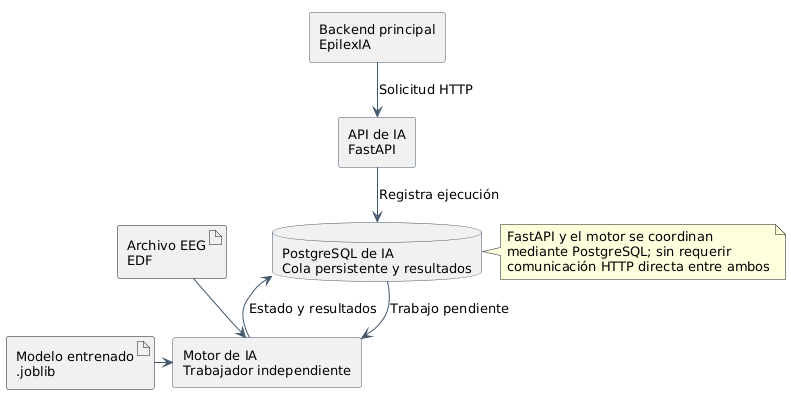
\includegraphics[width=\textwidth]{ThesisFigs/organizacion_procesamiento_ia_pgqueue.png}
    \caption{Organización del procesamiento de inteligencia artificial mediante cola persistente en EpilexIA.}
    \label{fig:organizacion-procesamiento-ia-pgqueue}
\end{figure}


\subsection{Preparación y procesamiento de señales EEG}
\label{subsec:preparacion-procesamiento-eeg-ia}

El procesamiento de señales electroencefalográficas mediante inteligencia artificial en EpilexIA parte de archivos digitales en formato EDF. El motor de inferencia accede al archivo asociado con la ejecución solicitada mediante una referencia a su ubicación en el almacenamiento, sin necesidad de transferir la totalidad de las muestras a través de la API de inteligencia artificial. Para interpretar el registro, el procedimiento utiliza la biblioteca MNE de Python.

El procedimiento de análisis forma parte del modelo de detección provisto por el equipo de ciencia de datos del proyecto, por lo que su diseño interno no integra el alcance del presente trabajo.
Para integrarlo, el motor considera sus etapas generales: la adaptación de las señales a un montaje bipolar longitudinal de 18 derivaciones, el remuestreo a 256~Hz, el filtrado, la segmentación en ventanas consecutivas de 10 segundos, la extracción de características de cada ventana y su normalización para cada registro.
La configuración de estas etapas se distribuye junto con el modelo entrenado, de modo que el motor aplica a cada estudio el mismo procedimiento con el que el modelo fue entrenado (Sección~\ref{subsec:modelo-vigente-hgb}).

El procesamiento se ejecuta de forma independiente de la navegación del especialista por la interfaz web. El trabajador obtiene las ejecuciones pendientes desde PostgreSQL, inicia el procedimiento de inferencia y actualiza la información de estado y resultados. Los intervalos temporales analizados se expresan en segundos relativos al inicio del registro, lo que permite relacionar las predicciones con las posiciones correspondientes dentro del estudio EEG.

Es importante distinguir este procedimiento del procesamiento realizado por el \textit{backend} clínico para la visualización de señales. Mientras este último prepara segmentos destinados a la recuperación y navegación temporal del registro, el motor de inteligencia artificial construye características de las ventanas y aplica el modelo predictivo para identificar intervalos que podrían requerir revisión clínica.


\subsection{Generación e interpretación de resultados}
\label{subsec:generacion-interpretacion-resultados-ia}

Para cada ventana analizada, el modelo entrega una probabilidad de crisis.
Estos valores constituyen salidas del modelo y no deben interpretarse, por sí solos, como una confirmación clínica de actividad epiléptica.

La decisión de señalar un intervalo combina dos parámetros: un umbral de probabilidad y una cantidad mínima de ventanas consecutivas que deben superarlo.
Ambos se definen en el paquete del modelo.
Al registrarse una ejecución, el umbral aplicable se incorpora a sus datos, de manera que el valor utilizado permanece asociado al procesamiento correspondiente aunque la configuración se modifique posteriormente.
Los valores del modelo vigente se indican en la Sección~\ref{subsec:modelo-vigente-hgb}.

Durante el análisis, el motor genera un archivo temporal con la información de las ventanas procesadas y registra en PostgreSQL únicamente las que integran un intervalo señalado.

Cada resultado conservado se vincula con su ejecución de origen e incluye el tiempo de inicio y fin del intervalo, expresados en segundos respecto del comienzo del registro, así como la probabilidad de crisis utilizada para su selección. La relación con la ejecución permite recuperar el estudio asociado y la información necesaria para identificar el procesamiento que produjo el resultado. Las ventanas se registran individualmente, por lo que un intervalo señalado se presenta como una secuencia de registros consecutivos.

La finalización satisfactoria de una ejecución indica que el procedimiento concluyó conforme a su flujo operativo, pero no implica necesariamente la existencia de resultados positivos almacenados. Si ninguna ventana satisface los criterios de selección, el procesamiento puede finalizar con estado exitoso y sin registros de resultados. Asimismo, los estados de ejecución permiten diferenciar los trabajos pendientes o en curso de aquellos que finalizan, fallan, exceden el tiempo permitido o son cancelados.

En consecuencia, los intervalos generados por el subsistema de inteligencia artificial deben entenderse como indicaciones de posibles hallazgos que orientan la revisión del registro EEG. Su interpretación requiere considerar las señales originales y el contexto clínico del estudio. La decisión sobre la relevancia de cada intervalo corresponde al especialista, por lo que el componente automatizado cumple una función de apoyo y no sustituye la evaluación médica.


\subsection{Integración de resultados en la revisión clínica}
\label{subsec:integracion-resultados-revision-clinica}

La integración de los resultados de inteligencia artificial en EpilexIA tiene como propósito facilitar que el especialista examine los intervalos identificados durante el procesamiento automatizado en el contexto del estudio electroencefalográfico. Para ello, el sistema relaciona cada ejecución con el estudio clínico correspondiente y permite recuperar los resultados mediante los servicios de integración entre el \textit{backend} clínico y la API de inteligencia artificial.

Una vez concluida la ejecución, el \textit{backend} clínico puede consultar las ventanas que cumplen los criterios de detección y obtener sus límites temporales. Estos intervalos se expresan en segundos respecto del inicio del registro EEG, lo que permite relacionarlos con la posición correspondiente en las señales visualizadas. De este modo, los resultados automatizados funcionan como referencias temporales para orientar la inspección del registro, sin sustituir la observación directa de las señales.

La revisión clínica conserva una separación entre los resultados producidos por el modelo y las decisiones del especialista. La identificación automática de un intervalo no implica que este haya sido confirmado como un evento epiléptico. Su relevancia debe determinarse mediante el análisis de la actividad electroencefalográfica y de la información clínica disponible para el estudio.

El diseño contempla mecanismos para incorporar a los informes médicos las ventanas de inteligencia artificial seleccionadas durante la revisión. La asociación conserva la referencia a la ejecución y al resultado de origen, así como información descriptiva y de clasificación aportada por el profesional. Esta vinculación permite distinguir los intervalos identificados automáticamente de aquellos que el especialista decide utilizar como parte de su informe.

Asimismo, EpilexIA permite registrar anomalías y anotaciones definidas manualmente por el especialista, incluso cuando no corresponden a una ventana previamente detectada por el modelo. Las anotaciones manuales y las ventanas de inteligencia artificial incluidas en un informe se gestionan como conjuntos diferenciados y pueden sincronizarse con el subsistema de IA mediante interfaces específicas. Por consiguiente, la ausencia de una detección automática no impide que el profesional documente un hallazgo observado durante la revisión.

La información de retroalimentación clínica se conserva en estructuras específicas del subsistema de inteligencia artificial. En particular, las inclusiones de ventanas en informes permiten mantener su asociación con la revisión profesional, mientras que las anotaciones manuales registran observaciones originadas en la evaluación del especialista. Estos datos podrían servir como insumos para procesos posteriores de mejora de los modelos, pero su almacenamiento no implica que EpilexIA ejecute automáticamente un reentrenamiento.

La organización de los informes mantiene la responsabilidad de cada especialista sobre el contenido clínico que elabora. Así, la consulta de resultados automatizados y la selección de ventanas para un informe se integran al flujo de trabajo médico sin convertir las predicciones en conclusiones diagnósticas obligatorias. La interpretación final y la elaboración del informe corresponden al profesional responsable.

En síntesis, la integración de resultados vincula las ejecuciones de inteligencia artificial con la navegación temporal del EEG, la documentación de hallazgos y la elaboración de informes médicos. El componente automatizado aporta referencias para la revisión, mientras que la valoración de su significado clínico permanece bajo el criterio del especialista.


\section{Diseño de seguridad y control de acceso}
\label{sec:seguridad-control-acceso}

El diseño de seguridad de EpilexIA contempla mecanismos destinados a controlar el acceso a las funcionalidades del sistema y a la información asociada con los pacientes, los estudios electroencefalográficos y los informes médicos. Dada la naturaleza de estos datos, el acceso se organiza mediante la identificación de los usuarios, la asignación de permisos y la verificación de las condiciones necesarias para realizar cada operación.

La autenticación se realiza a través del \textit{backend} clínico, que emite un \textit{token} de acceso para las sesiones válidas. Las solicitudes posteriores a los servicios protegidos incorporan dicho \textit{token}, cuya validez se comprueba antes de permitir el procesamiento de la operación. Este mecanismo se complementa con el registro de sesiones, lo que permite controlar la vigencia de los accesos autenticados.

La autorización combina permisos asociados a los roles del sistema con verificaciones adicionales sobre los recursos clínicos. Por ello, disponer de un permiso general para consultar o modificar estudios no implica necesariamente poder acceder a cualquier registro: determinadas operaciones también dependen de la relación del usuario con el estudio o el informe correspondiente.

En la aplicación web, las rutas y acciones disponibles se presentan de acuerdo con la autenticación y los permisos del usuario. Sin embargo, estas restricciones de interfaz no sustituyen las verificaciones realizadas por el \textit{backend}, que constituye el punto de control para autorizar las solicitudes recibidas.

Los siguientes apartados describen los mecanismos de autenticación, la organización de roles y permisos, las reglas de acceso a recursos clínicos y las consideraciones de protección de datos y comunicaciones contempladas en el diseño de EpilexIA.


\subsection{Autenticación de usuarios}
\label{subsec:autenticacion-usuarios}

La autenticación de usuarios en EpilexIA se realiza a través del \textit{backend} clínico y constituye el mecanismo de identificación previo al acceso a los servicios protegidos. El proceso comienza cuando el usuario introduce sus credenciales en la interfaz web. Estas se remiten al servicio de autenticación, que comprueba su validez y las condiciones de acceso de la cuenta antes de establecer una sesión.

Cuando las credenciales son válidas, el \textit{backend} genera un \textit{token} de acceso en formato \textit{JSON Web Token} (JWT).
 El \textit{token} se firma digitalmente e incorpora información que permite identificar al usuario y determinar su período de vigencia. Asimismo, contiene un identificador único de \textit{token}, denominado \texttt{jti}, que se utiliza para relacionarlo con un registro de sesión persistido en la base de datos clínica. La respuesta de autenticación proporciona al \textit{frontend} la información necesaria para continuar las operaciones del usuario, incluidos sus permisos.

En las solicitudes posteriores, la aplicación web incorpora el \textit{token} mediante el encabezado HTTP \texttt{Authorization}, utilizando el esquema \texttt{Bearer}. Antes de permitir el acceso a los servicios protegidos, el \textit{backend} comprueba la firma y la expiración del JWT, extrae su identificador \texttt{jti} y verifica que exista una sesión vigente asociada. Si alguna de estas condiciones no se cumple, la solicitud no se considera autenticada.

La configuración de seguridad utiliza una política de procesamiento HTTP sin estado, denominada \texttt{stateless}. Esto significa que la autenticación no depende de una sesión HTTP tradicional mantenida entre solicitudes. No obstante, EpilexIA conserva registros de sesiones de usuario en la base de datos, lo que permite controlar la vigencia de los \textit{tokens} emitidos y revocarlos antes de que alcancen su fecha de expiración.

Una vez validado el \textit{token}, el \textit{backend} recupera la información actual del usuario y las autoridades correspondientes a sus permisos. De esta manera, la autenticación establece la identidad del solicitante, mientras que la autorización posterior determina qué operaciones puede realizar. La validación de un JWT, por sí sola, no concede acceso indiscriminado a los recursos clínicos del sistema.

El cierre de sesión dispone de una operación específica que identifica el \textit{token} utilizado y elimina el registro de sesión correspondiente. En consecuencia, aunque el JWT conserve una firma válida y no haya alcanzado su expiración, deja de ser aceptado cuando ya no existe una sesión vigente asociada a su identificador. Asimismo, el procedimiento de restablecimiento de contraseña contempla la invalidación de sesiones para impedir la continuidad de accesos previamente autorizados.

El diseño también contempla procedimientos de activación de cuentas y restablecimiento de contraseñas mediante \textit{tokens} específicos, distintos de los JWT utilizados para acceder a los servicios clínicos. Estos mecanismos permiten gestionar el establecimiento o la recuperación de credenciales sin confundir dichas operaciones con una sesión autenticada de uso ordinario.

En conjunto, la autenticación de EpilexIA combina la verificación de credenciales, la emisión de \textit{tokens} firmados y el control de sesiones persistidas. Esta organización proporciona una base para identificar a los usuarios y aplicar posteriormente las reglas de roles, permisos y acceso contextual a los recursos clínicos, desarrolladas en los siguientes apartados.


\subsection{Roles y permisos}
\label{subsec:roles-permisos}

El control de acceso de EpilexIA se organiza mediante un esquema de autorización basado en roles y permisos. Cada usuario dispone de un rol asociado con un conjunto de operaciones autorizadas, de acuerdo con las responsabilidades que desempeña dentro del sistema. Esta organización permite diferenciar las funciones administrativas, el registro y la preparación de estudios, y las actividades de revisión clínica.

El modelo vigente contempla tres roles: Administrador, Técnico y Especialista. El Administrador se orienta a la gestión de usuarios, roles y permisos, además de las operaciones de supervisión y administración disponibles en el sistema. El Técnico participa principalmente en el registro de pacientes y estudios electroencefalográficos, así como en la incorporación de los archivos correspondientes. El Especialista desarrolla las tareas clínicas de consulta y revisión de estudios, análisis de señales, registro de hallazgos y elaboración de informes médicos.

El Cuadro~\ref{tab:roles-permisos-epilexia} resume las responsabilidades principales de estos perfiles. Se trata de una descripción funcional de los roles, no de una enumeración exhaustiva de todas las autorizaciones almacenadas en la base de datos.

\begin{table}[H]
\centering
\caption{Responsabilidades principales de los roles de EpilexIA.}
\label{tab:roles-permisos-epilexia}
\small
\begin{tabular}{|p{0.20\textwidth}|p{0.68\textwidth}|}
\hline
\textbf{Rol} & \textbf{Responsabilidades principales} \\ \hline
Administrador & Gestión de usuarios, roles y permisos; acceso administrativo y supervisión de los recursos del sistema conforme a las autorizaciones disponibles. \\ \hline
Técnico & Registro y actualización de información de pacientes, creación de estudios EEG e incorporación de archivos asociados a los estudios en los que participa. \\ \hline
Especialista & Consulta y revisión de estudios EEG, análisis de señales, registro de anomalías y eventos, y creación y gestión de informes médicos conforme a los permisos y reglas de acceso aplicables. \\ \hline
\end{tabular}
\end{table}

Los permisos se representan mediante identificadores asociados a recursos y acciones. Por ejemplo, \texttt{patients.list}, \texttt{studies.create}, \texttt{reports.update} y \texttt{anomalies.create} expresan autorizaciones para consultar pacientes, registrar estudios, actualizar informes y crear anomalías, respectivamente. Esta separación permite controlar operaciones concretas sin depender exclusivamente del nombre del rol.

La relación entre roles y permisos se mantiene en la base de datos clínica. Al autenticarse, el usuario recibe información sobre sus permisos, que la aplicación web utiliza para habilitar rutas y presentar las acciones correspondientes. En el \textit{backend}, los permisos se traducen en autoridades de seguridad y se verifican en los servicios protegidos antes de ejecutar las operaciones solicitadas.

La asignación de permisos puede administrarse mediante las funcionalidades destinadas a la gestión de roles. Por ello, el conjunto de acciones disponible para un usuario depende de las autorizaciones efectivamente asociadas a su rol, y no únicamente de la denominación de este. Las asignaciones iniciales previstas en los \textit{scripts} de base de datos constituyen una configuración de referencia que puede diferir de la existente en una instalación administrada.

Es importante distinguir los permisos funcionales de las condiciones de acceso a un registro particular. Por ejemplo, disponer de autorización para consultar estudios no implica necesariamente poder visualizar cualquier estudio EEG. El sistema aplica comprobaciones adicionales según la participación del usuario y su relación con el recurso solicitado. Estas reglas de autorización contextual se desarrollan en el apartado siguiente.

De esta manera, la organización por roles y permisos proporciona un mecanismo para distribuir responsabilidades y restringir las operaciones disponibles, mientras que las verificaciones específicas sobre pacientes, estudios e informes complementan el control de acceso a la información clínica.


\subsection{Autorización sobre recursos clínicos}
\label{subsec:autorizacion-recursos-clinicos}

La autorización sobre recursos clínicos en EpilexIA complementa los permisos asociados a los roles mediante verificaciones relacionadas con el registro solicitado. Este mecanismo permite distinguir entre disponer de autorización para ejecutar una operación y estar habilitado para realizarla sobre un paciente, estudio electroencefalográfico o informe determinado. Las comprobaciones se efectúan en el \textit{backend} clínico, de manera que la presentación de acciones en la interfaz web no constituye por sí sola una autorización suficiente.

En los servicios vinculados a estudios EEG, el control de acceso considera la relación del usuario con cada estudio. La consulta se permite al Administrador, al Técnico que registró el estudio, al Especialista responsable y a los especialistas incorporados como observadores, siempre que dispongan también de los permisos funcionales requeridos. Por el contrario, un Especialista que no mantiene una relación autorizada con el estudio no adquiere acceso únicamente por pertenecer al mismo rol clínico.

Las operaciones de modificación de los datos del estudio están sujetas a condiciones más restrictivas. De acuerdo con las reglas de acceso implementadas, estas operaciones se habilitan al Administrador o al Especialista responsable, según los permisos correspondientes. La condición de observador permite participar en la revisión del estudio, pero no otorga por sí misma autorización para modificar sus datos generales. Asimismo, el Técnico que registró el estudio no adquiere por ese hecho las facultades de modificación reservadas a otros participantes.

La incorporación de archivos asociados al estudio utiliza una comprobación específica. Además del permiso requerido para la operación, pueden realizar la carga el Administrador, el Especialista responsable y el Técnico creador del estudio. Esta capacidad se encuentra condicionada por el estado del registro: los estudios anulados no admiten nuevas cargas. De esta manera, la autorización considera tanto la relación del usuario con el estudio como las condiciones de la operación solicitada.

En el visualizador EEG, el acceso a señales, segmentos y otros recursos del estudio se apoya en las reglas de consulta previamente descritas. Por su parte, el registro y la modificación de anomalías y eventos EEG requieren permisos específicos y verificaciones adicionales sobre la participación del usuario. Esta separación evita equiparar la capacidad de observar las señales con la autorización para modificar los hallazgos asociados al estudio.

La gestión de informes médicos incorpora un control adicional basado en la autoría. EpilexIA permite que distintos especialistas vinculados a un mismo estudio elaboren informes propios. La relación entre el estudio, el informe y su autor se conserva en los registros correspondientes, y el sistema establece que cada especialista puede disponer de un único informe propio por estudio. Por tanto, tanto el Especialista responsable como los Especialistas incorporados como observadores autorizados pueden elaborar sus propios informes médicos asociados al estudio, siempre que dispongan de los permisos correspondientes. Cada informe pertenece al Especialista que lo creó y no puede ser modificado por otros profesionales.


La consulta de un informe perteneciente a otro profesional no implica autorización para modificarlo. Cuando un especialista accede a un informe ajeno mediante los servicios vinculados al estudio, la información se presenta en modo de solo lectura. La edición del informe propio requiere, además de los permisos funcionales, que se cumplan las condiciones relativas a su autoría y estado. La creación de nuevos informes también está condicionada por las reglas del proceso, entre ellas la inexistencia de un informe propio previo y las restricciones asociadas al cierre de informes del estudio.

En cuanto a los datos de pacientes, la autorización se organiza principalmente mediante permisos funcionales de consulta, creación y actualización. A diferencia de las comprobaciones contextuales aplicadas a los estudios, las operaciones generales sobre pacientes no se restringen al Técnico creador ni al Especialista asignado: dependen únicamente de los permisos del usuario. Esta distinción es relevante para describir con precisión el alcance de las verificaciones presentes en cada servicio.

Finalmente, las reglas de acceso contextual se aplican en los servicios que incorporan expresamente dichas comprobaciones. Algunas operaciones generales de búsqueda y exportación utilizan controles basados en permisos sin reproducir necesariamente todas las restricciones de participación de los servicios asociados a un estudio particular. Por ello, el diseño de seguridad debe analizarse considerando conjuntamente las autoridades exigidas por cada interfaz y las verificaciones adicionales realizadas por su lógica de aplicación.

En síntesis, la autorización sobre recursos clínicos combina permisos funcionales, relaciones de participación y condiciones propias de los registros. Esta organización permite diferenciar la consulta de estudios, la modificación de datos, la incorporación de archivos y la gestión de informes, manteniendo la responsabilidad de las decisiones clínicas en los especialistas habilitados.


\subsection{Protección de datos y comunicaciones}
\label{subsec:proteccion-datos-comunicaciones}

La protección de la información en EpilexIA comprende tanto los datos clínicos almacenados como las comunicaciones entre los componentes de la plataforma. Debido a que el sistema gestiona información de pacientes, registros electroencefalográficos, archivos de video e informes médicos, su diseño combina controles de acceso de aplicación con mecanismos de separación de servicios y medidas que deben completarse en el entorno de despliegue.

En el tratamiento de las credenciales, el sistema distingue las contraseñas utilizadas para autenticar a los usuarios de los \textit{tokens} de acceso emitidos para las sesiones. La creación y recuperación de cuentas se realizan mediante procedimientos específicos de activación y restablecimiento de contraseña. Por su parte, las solicitudes autenticadas utilizan \textit{tokens} JWT, cuya validación y revocación se describieron en el apartado~\ref{subsec:autenticacion-usuarios}. Estos mecanismos evitan que la autorización de las operaciones clínicas dependa únicamente de los controles visibles en la interfaz web.

La comunicación habitual comienza en el navegador y pasa por el servidor web Nginx, que entrega la aplicación y encamina las solicitudes hacia el \textit{backend} clínico. Este último centraliza la autenticación, la autorización y el acceso a los recursos clínicos. La comunicación con el subsistema de inteligencia artificial se realiza mediante una interfaz de servicio diferenciada, que utiliza autenticación HTTP Basic con credenciales configuradas para la integración. En consecuencia, las credenciales del usuario clínico y las empleadas entre servicios cumplen funciones distintas.

El cifrado de las comunicaciones constituye una consideración específica del despliegue. El uso de HTTPS con TLS permite proteger la información transmitida entre el navegador y el punto de entrada del sistema frente a su lectura o alteración durante el transporte. En el entorno de despliegue utilizado, el acceso de los usuarios se realiza mediante HTTPS (Sección~\ref{subsec:despliegue-nube}), mientras que los servicios internos se comunican dentro de la red del propio entorno. La habilitación de HTTPS y la configuración de los certificados forman parte de la instalación en cada infraestructura donde se despliegue EpilexIA.

Los datos estructurados se conservan en bases PostgreSQL diferenciadas: una destinada a los registros clínicos y otra a las ejecuciones y resultados del subsistema de inteligencia artificial. Los archivos EEG y de video se mantienen en almacenamiento persistente separado de las tablas relacionales. De igual manera, los artefactos de los modelos de aprendizaje automático se alojan en recursos de archivos accesibles para los componentes que ejecutan las inferencias. Esta distribución permite administrar por separado los registros, los archivos de gran tamaño y los modelos utilizados.

La persistencia de estos recursos requiere medidas operativas adicionales. El diseño de despliegue mediante contenedores y volúmenes permite conservar la información aunque se detengan o reinicien los servicios, pero no reemplaza la necesidad de realizar copias de seguridad. Los recursos críticos del sistema son el almacenamiento de EEG y video, la base clínica y la base de inteligencia artificial, cuya conservación y respaldo deben contemplarse en la administración de la infraestructura.

La configuración de los servicios también incluye información sensible, como las credenciales de conexión a las bases de datos, la clave utilizada para firmar JWT y las credenciales de integración con la API de inteligencia artificial. Estos valores deben gestionarse en el entorno de operación y no incorporarse al contenido público de la aplicación web ni a la documentación distribuida. La protección efectiva de tales parámetros depende asimismo de las restricciones de acceso al servidor y a su configuración.

En cuanto al seguimiento técnico, EpilexIA dispone de mecanismos de registro que permiten relacionar solicitudes y operaciones mediante identificadores de trazabilidad. Las contraseñas y los \textit{tokens} se enmascaran en los registros estructurados. No obstante, la disponibilidad de estos registros no sustituye la aplicación de controles de acceso a los propios archivos de auditoría ni las políticas de conservación de información clínica.

En síntesis, el diseño de protección de datos y comunicaciones combina autenticación, autorización, separación de componentes, almacenamiento persistente y trazabilidad de operaciones. Su efectividad requiere complementar los controles implementados en la aplicación con una configuración segura de red, cifrado de transporte, gestión de credenciales y procedimientos de respaldo adecuados al entorno institucional de operación.

\section{Diseño de auditoría y trazabilidad}
\label{sec:diseno-auditoria-trazabilidad}

El diseño de auditoría y trazabilidad de EpilexIA contempla mecanismos para registrar operaciones relevantes del sistema y facilitar el seguimiento de las actividades realizadas sobre sus recursos. Dado que la plataforma administra información de pacientes, estudios electroencefalográficos e informes médicos, resulta necesario disponer de registros que permitan reconocer las acciones efectuadas y el contexto en el que se produjeron.

La auditoría funcional se apoya en eventos persistidos en la base de datos clínica. Estos registros permiten identificar operaciones de negocio seleccionadas y conservar información sobre el actor, la acción realizada y los datos de contexto correspondientes. Su consulta proporciona una visión histórica de las actividades registradas, sin que ello implique que todas las solicitudes HTTP o todos los cambios internos generen necesariamente un evento de auditoría persistente.

Para facilitar la revisión de esta información, EpilexIA incorpora una vista de actividad reciente en el panel de control y una interfaz de consulta de auditorías. Esta última permite explorar los registros mediante paginación, ordenamiento cronológico y filtros combinables, de acuerdo con las autorizaciones exigidas por los servicios del \textit{backend}.

De manera complementaria, los componentes de aplicación producen registros técnicos que permiten seguir solicitudes y diagnosticar incidencias. Estos registros utilizan identificadores de trazabilidad para relacionar las etapas de una operación. En el subsistema de inteligencia artificial, el identificador de ejecución permite además vincular el seguimiento técnico con los estados y resultados del procesamiento asíncrono.

Por tanto, el diseño distingue entre los eventos de auditoría conservados para la consulta funcional y los registros técnicos utilizados para el seguimiento operativo. Los siguientes apartados describen el registro de operaciones y eventos, los mecanismos de consulta de auditorías y la trazabilidad de procesos e integraciones entre componentes.


\subsection{Registro de operaciones y eventos}
\label{subsec:registro-operaciones-eventos}

El registro de operaciones y eventos en EpilexIA tiene como finalidad conservar información sobre determinadas actividades realizadas dentro del sistema, permitiendo identificar las acciones ejecutadas y el contexto en el que se produjeron. Este mecanismo constituye una parte de la auditoría funcional y proporciona información para la revisión posterior de las operaciones relacionadas con los recursos administrados por la plataforma.

La implementación de auditoría se encuentra integrada en el \textit{backend}
clínico. Para identificar las operaciones de negocio que generan
eventos de auditoría persistentes, el sistema utiliza la enumeración
\texttt{AuditEventType}. Estos eventos son publicados por los servicios
de aplicación y procesados mediante componentes específicos que
permiten conservarlos en la base de datos clínica.

De manera complementaria, el \textit{backend} utiliza la enumeración
\texttt{LogAction} para identificar operaciones registradas mediante
el mecanismo de \textit{logging} estructurado. Este mecanismo proporciona
trazas técnicas para el seguimiento de solicitudes y operaciones,
pero no implica necesariamente la generación de un evento de
auditoría persistente.

El registro de auditoría contempla operaciones relacionadas con la administración del sistema y la gestión de sus recursos. Entre ellas se encuentran determinadas acciones sobre usuarios, pacientes, estudios electroencefalográficos e informes médicos. La generación de estos registros depende de los puntos de la aplicación en los que se encuentra incorporado el mecanismo de auditoría, por lo que no debe interpretarse como un registro automático y exhaustivo de todas las solicitudes recibidas por el \textit{backend}.

Para conservar la información de los eventos, EpilexIA utiliza estructuras persistentes en la base de datos clínica PostgreSQL. Los registros de auditoría permiten asociar una operación con información contextual, como el usuario que la realizó, la acción registrada y el momento en que ocurrió. Según el tipo de evento, también pueden incorporarse referencias a los recursos involucrados y otros datos necesarios para describir la actividad.

La implementación incorpora componentes específicos para intervenir en el registro de eventos, entre ellos \texttt{AuditEventRecordListener}. Este componente forma parte del mecanismo utilizado por el \textit{backend} para gestionar la información de auditoría. Su participación debe distinguirse de los registros técnicos generales, ya que estos últimos están destinados principalmente al diagnóstico y seguimiento operativo de los servicios.

La conservación de eventos en la base de datos permite consultar posteriormente las actividades registradas sin depender exclusivamente de los mensajes producidos durante la ejecución de la aplicación. Esta persistencia facilita la construcción de vistas de actividad y servicios de consulta que recuperan los registros conforme a los criterios solicitados.

Es importante señalar que la existencia de un registro de auditoría no implica necesariamente que se conserve una copia completa del contenido anterior y posterior de cada recurso modificado. El alcance de la información disponible depende de los datos registrados para cada operación. Por esta razón, los eventos deben interpretarse como evidencias de actividades específicas y no como un mecanismo general de reconstrucción de todos los estados históricos del sistema.

Asimismo, el registro de una operación no sustituye las verificaciones de autenticación y autorización. Los controles de acceso determinan si una solicitud puede ejecutarse, mientras que la auditoría permite conservar información sobre las actividades para las cuales se ha previsto su registro. Ambos mecanismos cumplen funciones complementarias dentro del diseño de seguridad de EpilexIA.

En conjunto, el registro de operaciones y eventos proporciona una base persistente para el seguimiento de las actividades relevantes del sistema. Su integración con los servicios de consulta permite que los usuarios autorizados examinen posteriormente los eventos almacenados, identifiquen las operaciones registradas y dispongan de información contextual para su revisión.


\subsection{Consulta y seguimiento de auditorías}
\label{subsec:consulta-seguimiento-auditorias}

La consulta de auditorías en EpilexIA permite recuperar y examinar las operaciones registradas por el sistema, proporcionando información sobre las actividades realizadas y su contexto. Esta funcionalidad complementa el mecanismo de registro de eventos descrito anteriormente y facilita la revisión de las acciones ejecutadas sobre los recursos de la plataforma.

El sistema dispone de una vista de actividad reciente integrada en el panel de control, destinada a presentar un resumen de las operaciones registradas. Esta visualización permite identificar acontecimientos recientes sin necesidad de acceder inicialmente a la consulta completa de auditorías.


La Figura~\ref{fig:actividad-reciente} ilustra esta funcionalidad mediante una lista de operaciones registradas, acompañadas de sus respectivas fechas y horas. Asimismo, se observa el acceso a la consulta completa de auditorías.

\begin{figure}[H]
    \centering
    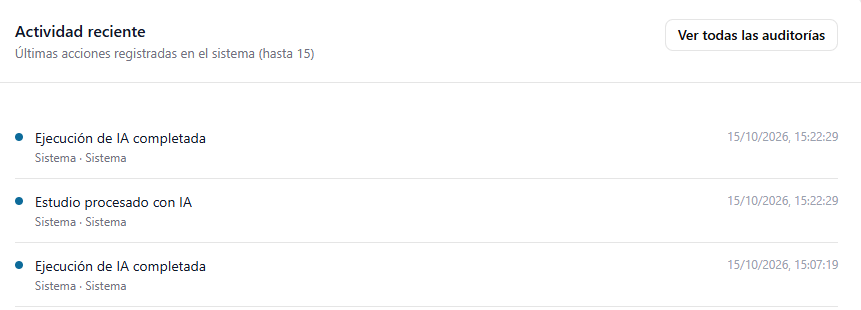
\includegraphics[width=0.90\textwidth]{ThesisFigs/actividad_reciente_epilexia.png}
    \caption{Vista de actividad reciente en el panel de control de EpilexIA.}
    \label{fig:actividad-reciente}
\end{figure}


Para una revisión más detallada, EpilexIA incorpora la interfaz denominada ``Ver todas las auditorías'', que permite consultar los registros mediante una tabla organizada. Esta interfaz presenta información de las operaciones registradas, incluyendo datos relacionados con el usuario, su rol, la acción realizada y la fecha del evento, según los atributos disponibles en cada registro.

La consulta contempla mecanismos de filtrado que permiten restringir los resultados conforme a diferentes criterios. Entre ellos se encuentran la búsqueda por usuario, la selección de roles y acciones, y la delimitación de fechas. La combinación de estos filtros facilita la localización de actividades específicas dentro del conjunto de registros disponibles.


En particular, el filtrado por fecha utiliza un control de selección que permite indicar el día de interés, mientras que la selección de roles se realiza mediante las opciones disponibles en el sistema. Estos controles reducen la necesidad de introducir manualmente determinados valores y contribuyen a mantener criterios de búsqueda consistentes.

Los resultados se presentan mediante paginación, de manera que la interfaz recupera y muestra una cantidad limitada de registros por página. Este mecanismo evita presentar simultáneamente la totalidad de los eventos almacenados y facilita la navegación entre los resultados de una consulta. Asimismo, el ordenamiento permite organizar los registros conforme a los criterios admitidos por el servicio, incluyendo su secuencia temporal.


La Figura~\ref{fig:consulta-auditorias} presenta
la interfaz de consulta de auditorías de EpilexIA.
En ella se observan los registros de actividad
organizados por fecha y hora, evento, actor,
rol y contexto, junto con los controles de
filtrado y paginación disponibles.


\begin{figure}[H]
    \centering
    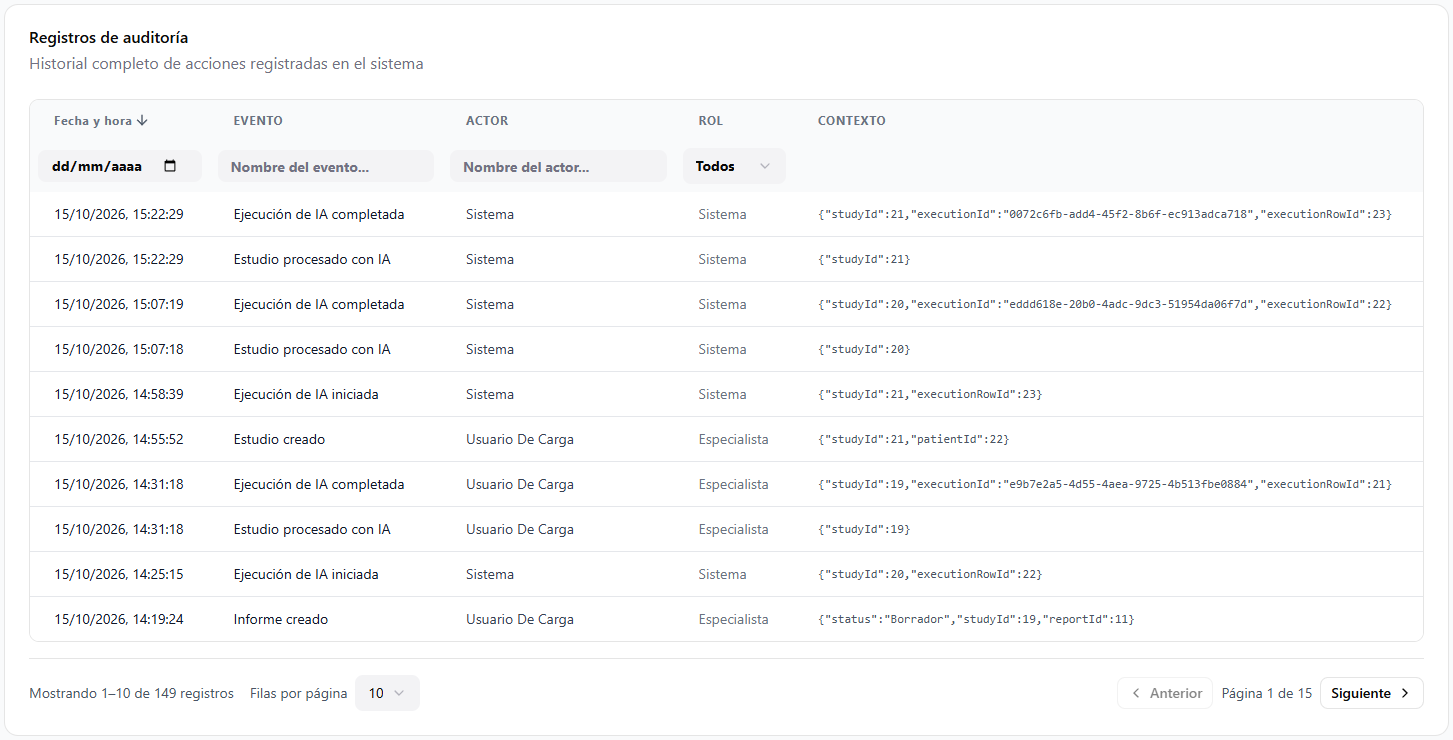
\includegraphics[width=\textwidth]{ThesisFigs/consulta_auditorias_epilexia.png}
    \caption{Consulta, filtrado y paginación de auditorías en EpilexIA.}
    \label{fig:consulta-auditorias}
\end{figure}


La recuperación de la información se realiza mediante servicios REST del \textit{backend} clínico. Estos servicios reciben los parámetros de búsqueda y paginación, consultan los registros disponibles y devuelven los resultados correspondientes a la aplicación web. El procesamiento de los criterios de consulta en el servidor permite mantener una separación entre la presentación de los datos y la lógica encargada de recuperarlos.

El acceso a las funcionalidades de auditoría se encuentra sujeto a los permisos definidos para los usuarios del sistema. La interfaz web presenta las opciones correspondientes a las autorizaciones disponibles, mientras que el \textit{backend} verifica los permisos requeridos antes de responder a las solicitudes de consulta.

Es importante señalar que la información presentada corresponde a los eventos efectivamente registrados por los mecanismos de auditoría de EpilexIA. Por consiguiente, la ausencia de una actividad en los resultados de búsqueda no demuestra, por sí sola, que ninguna operación relacionada haya ocurrido, dado que el alcance del registro depende de los eventos contemplados por la aplicación.

En conjunto, la consulta y el seguimiento de auditorías proporcionan herramientas para examinar las actividades registradas, localizar operaciones mediante filtros y navegar por los resultados de manera organizada. Estas funcionalidades contribuyen a la supervisión administrativa y complementan los mecanismos de seguridad y trazabilidad del sistema.

% FIGURA OPCIONAL: activar después de subir la imagen a ThesisFigs.
% La Figura~\ref{fig:consulta-auditorias-epilexia} presenta la interfaz de consulta de auditorías.
% \begin{figure}[H]
%     \centering
%     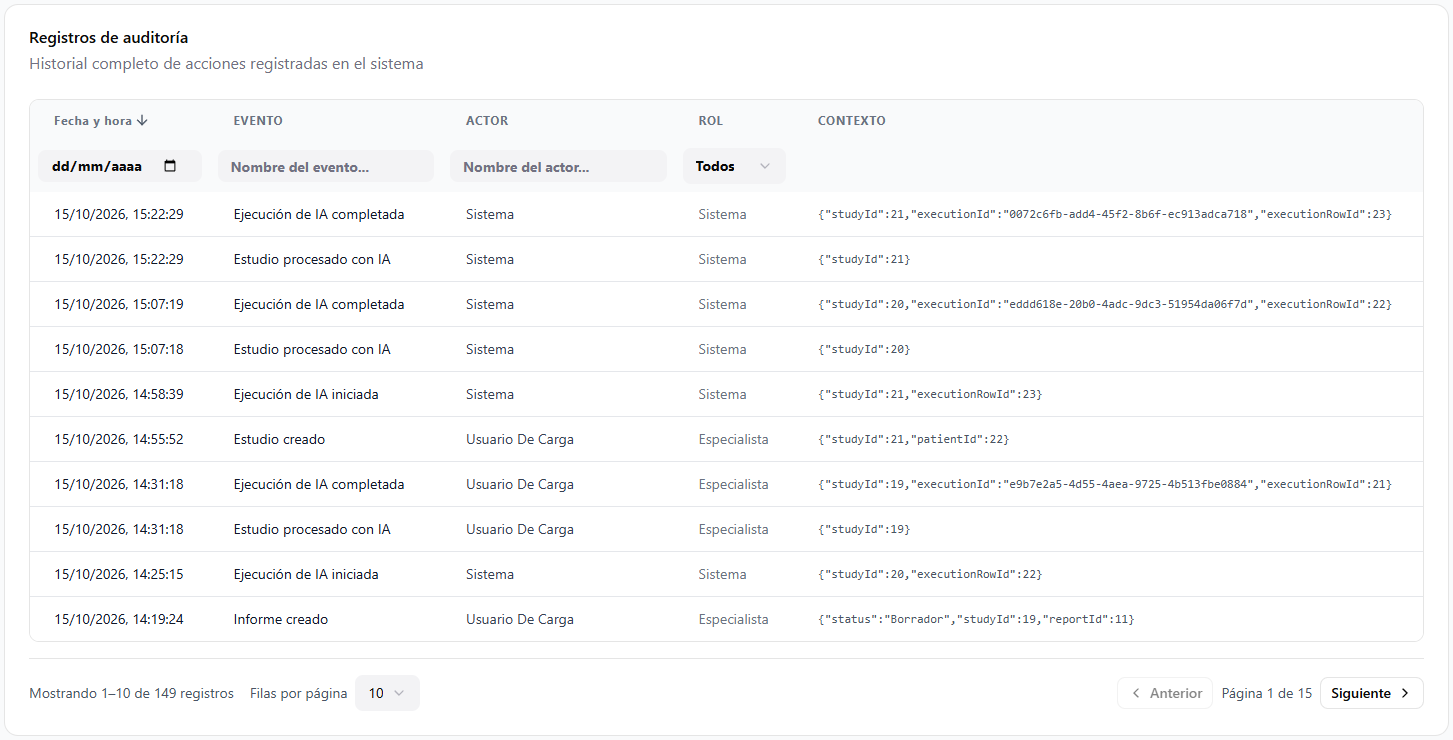
\includegraphics[width=\textwidth]{ThesisFigs/consulta_auditorias_epilexia.png}
%     \caption{Interfaz de consulta y filtrado de auditorías del sistema EpilexIA.}
%     \label{fig:consulta-auditorias-epilexia}
% \end{figure}


\subsection{Trazabilidad de procesos e integración}
\label{subsec:trazabilidad-procesos-integracion}

La trazabilidad de procesos en EpilexIA comprende los mecanismos
que permiten relacionar las solicitudes recibidas por los
servicios de aplicación con las operaciones ejecutadas por
sus distintos componentes. Esta capacidad resulta especialmente
relevante en los procedimientos que involucran varias etapas
de procesamiento o requieren comunicación entre servicios
independientes.

En el \textit{backend} clínico, los registros técnicos permiten
conservar información sobre el procesamiento de solicitudes
y las incidencias que pueden producirse durante su ejecución.
Para facilitar su seguimiento, se utilizan identificadores
de trazabilidad que permiten relacionar los mensajes
correspondientes a una misma operación. Estos registros
cumplen una función operativa y deben distinguirse de los
eventos de auditoría funcional almacenados en la base de
datos clínica.

La integración con el subsistema de inteligencia artificial
incorpora un mecanismo adicional de identificación. Cada
solicitud de procesamiento aceptada se asocia con un
identificador de ejecución, denominado
\texttt{executionId}, que permite reconocer el trabajo
correspondiente durante las distintas etapas de su ciclo
de vida. Este identificador constituye una referencia
para consultar el estado del procesamiento y recuperar
los resultados generados.

La API de inteligencia artificial registra la ejecución
en su base de datos PostgreSQL. Posteriormente, el motor
independiente obtiene los trabajos pendientes, realiza
el procesamiento de las señales EEG y actualiza la
información correspondiente a sus estados y resultados.
La persistencia de estos registros permite seguir
el avance del trabajo sin depender de una conexión
HTTP continua entre la API y el motor. La organización
de estos componentes y su mecanismo de coordinación
mediante PostgreSQL se ilustran en la
Figura~\ref{fig:organizacion-procesamiento-ia-pgqueue}.


El seguimiento de las ejecuciones contempla estados
que permiten diferenciar los trabajos pendientes,
aquellos que se encuentran en procesamiento y los
que han finalizado. Asimismo, se consideran situaciones
de fallo, cancelación o superación del tiempo permitido.
Esta información permite distinguir entre la aceptación
inicial de una solicitud y la finalización efectiva
del análisis automatizado.

La relación entre los componentes también se apoya
en los identificadores de los estudios clínicos.
El \textit{backend} clínico conserva la información del
estudio EEG, mientras que el subsistema de inteligencia
artificial registra las ejecuciones y los resultados
asociados mediante referencias lógicas. Dado que
ambos subsistemas utilizan bases de datos independientes,
estas referencias permiten establecer la correspondencia
entre sus registros sin requerir claves foráneas
entre las dos bases de datos.

Los resultados del procesamiento mantienen su
asociación con la ejecución que los produjo. De esta
manera, es posible identificar el análisis de origen
de los intervalos detectados y relacionarlos con el
estudio electroencefalográfico correspondiente. Esta
vinculación facilita la recuperación de información
desde los servicios de integración y su presentación
durante la revisión clínica.

De forma complementaria, los eventos de auditoría
funcional permiten conservar determinadas acciones
relacionadas con el inicio y la finalización de
procesamientos de inteligencia artificial, cuando
estas operaciones se encuentran contempladas por
los mecanismos de registro del \textit{backend}. Su finalidad
es documentar actividades relevantes para la consulta
posterior, mientras que los estados de ejecución y
los registros técnicos proporcionan información
más específica para el seguimiento operativo.

Es importante señalar que estos mecanismos no
constituyen necesariamente una traza única y completa
de todas las operaciones realizadas por los componentes.
El nivel de detalle disponible depende de los
identificadores propagados, los registros generados
por cada servicio y los eventos efectivamente
persistidos durante el procesamiento.

En conjunto, la trazabilidad de procesos e integración
de EpilexIA combina identificadores de solicitudes,
referencias a estudios clínicos, identificadores de
ejecución y registros de estado. Esta organización
facilita el seguimiento de los procedimientos
distribuidos, la identificación de incidencias y
la relación entre las operaciones técnicas y los
recursos clínicos involucrados.


\section{Diseño de interfaz de usuario}
\label{sec:diseno-interfaz-usuario}

El diseño de la interfaz de usuario de EpilexIA se orienta a facilitar la interacción de los distintos perfiles con las funcionalidades del sistema. Para ello, considera las necesidades de administración, de registro y gestión de estudios electroencefalográficos, de identificación de pacientes durante la creación de estudios y de revisión clínica.

La organización de la interfaz contempla los tres
roles definidos en el sistema: Administrador, Técnico
y Especialista. Cada perfil dispone de opciones de
navegación y acciones relacionadas con sus permisos,
de manera que las funcionalidades presentadas
correspondan a las tareas que puede desempeñar.
Esta diferenciación contribuye a organizar el acceso
a los recursos y a reducir la exposición de opciones
que no forman parte de las responsabilidades del
usuario.

La aplicación web se desarrolla mediante React y
utiliza componentes reutilizables para estructurar
las pantallas, los formularios, las tablas de datos
y los controles de interacción. Su diseño contempla
la adaptación de los elementos visuales a diferentes
dimensiones de pantalla, procurando mantener una
distribución adecuada de la información y facilitar
la navegación entre las funcionalidades disponibles.

Una parte central del diseño corresponde a la
visualización de estudios EEG. Debido a la naturaleza
temporal de las señales electroencefalográficas,
esta interfaz incorpora mecanismos de navegación
por el registro, selección de montajes, ajuste de
filtros y sensibilidad, así como opciones para ampliar
el área de visualización. Estos controles permiten
al especialista examinar las señales y relacionarlas
con los eventos y hallazgos asociados al estudio.


El diseño también contempla la presentación de los resultados de inteligencia artificial disponibles para cada estudio. Los intervalos registrados se integran en el entorno de revisión clínica como información complementaria, permitiendo al Especialista consultar las señales correspondientes y determinar su relevancia. Asimismo, la interfaz facilita el registro de anomalías, eventos y la elaboración de informes médicos vinculados al estudio.


En las operaciones de administración y gestión,
la interfaz utiliza formularios, tablas y mecanismos
de búsqueda para facilitar la consulta y actualización
de la información. Estas funcionalidades se complementan
con mensajes de estado y controles de interacción
que permiten comunicar al usuario el resultado de
las operaciones realizadas.

Los siguientes apartados describen la organización
general de la interfaz, las pantallas destinadas
a la administración y gestión de estudios, el
visualizador EEG y los componentes utilizados
para la revisión clínica y elaboración de informes.


\subsection{Organización general de la interfaz}
\label{subsec:organizacion-general-interfaz}

La interfaz web de EpilexIA se organiza mediante
pantallas destinadas a las principales actividades
del sistema. Su estructura permite que los usuarios
accedan a las funcionalidades correspondientes a
su perfil y mantengan una navegación consistente
entre las operaciones de administración, gestión
de estudios y revisión clínica.

El acceso a la aplicación comienza con una pantalla
de autenticación, desde la cual el usuario introduce
sus credenciales. Una vez completado el proceso
de identificación, el sistema presenta el entorno
de trabajo correspondiente a los permisos asociados
a su cuenta. Esta organización permite diferenciar
las opciones disponibles sin requerir interfaces
completamente independientes para cada perfil.

El panel de control constituye el punto de entrada
a las funcionalidades del sistema. Su contenido
se organiza mediante elementos de resumen y accesos
a las operaciones habituales del usuario. De acuerdo
con el perfil autenticado, pueden presentarse
indicadores relacionados con pacientes, estudios
electroencefalográficos, informes médicos y
procesamientos mediante inteligencia artificial,
así como accesos a las secciones habilitadas.


La Figura~\ref{fig:panel-principal-especialista}
presenta la organización del panel de control de
EpilexIA correspondiente al perfil Especialista.
En ella se observan los indicadores de resumen,
los accesos rápidos a las funcionalidades
disponibles y la sección de actividad reciente.


\begin{figure}[H]
    \centering
    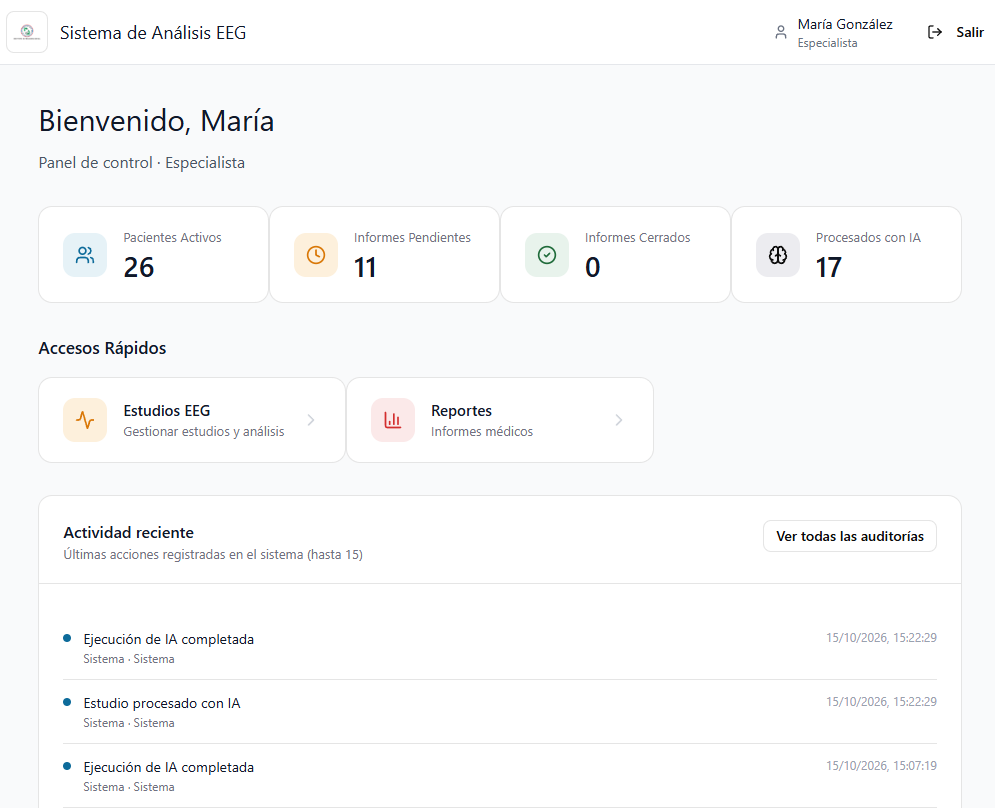
\includegraphics[width=\textwidth]{ThesisFigs/panel_principal_especialista.png}
    \caption{Organización del panel de control de EpilexIA
    correspondiente al perfil Especialista.}
    \label{fig:panel-principal-especialista}
\end{figure}


La navegación se estructura alrededor de las principales entidades y procesos administrados por EpilexIA. Las interfaces de estudios reúnen las operaciones relacionadas con su registro, seguimiento y acceso a los archivos asociados. Durante la creación de un estudio, el usuario puede seleccionar un paciente existente o registrar uno nuevo. Desde el entorno de un estudio, los usuarios autorizados pueden acceder a las funcionalidades de visualización de señales y revisión clínica.

La presentación de las acciones considera los
permisos del usuario autenticado. Por ejemplo,
las operaciones administrativas se orientan al
perfil Administrador, las actividades de registro
y preparación de estudios corresponden principalmente
al Técnico, y las herramientas de análisis e
informes médicos se destinan al Especialista.
Esta diferenciación se refleja en los accesos,
controles y operaciones disponibles en cada pantalla.

Para mantener una experiencia de navegación
uniforme, la aplicación utiliza componentes
reutilizables en la presentación de información.
Entre ellos se encuentran tablas de registros,
formularios, controles de búsqueda, botones
de acción y elementos de navegación. La utilización
de estos componentes favorece la consistencia
visual y funcional entre las diferentes secciones
del sistema.

Las pantallas que presentan conjuntos de registros
incorporan mecanismos de búsqueda y organización
de resultados, según las características de cada
funcionalidad. Asimismo, los formularios permiten
introducir o actualizar información mediante
campos y controles específicos. Estas operaciones
se complementan con mecanismos de validación
y mensajes que comunican al usuario el estado
de las solicitudes realizadas.

La organización de la interfaz también considera
la adaptación a diferentes dimensiones de pantalla.
Para ello, la distribución de los elementos se
ajusta según el espacio disponible, procurando
conservar la accesibilidad de los controles y
la legibilidad de la información. No obstante,
las funcionalidades de análisis de señales EEG
requieren una superficie de visualización adecuada
debido a la cantidad de información gráfica
presentada simultáneamente.

En conjunto, esta organización proporciona
una estructura común para las distintas actividades
de EpilexIA y permite integrar la gestión
administrativa, el registro de estudios y la
revisión clínica dentro de una misma aplicación
web. Las características particulares de las
interfaces correspondientes a estos procesos
se desarrollan en los siguientes apartados.


\subsection{Interfaces de administración y gestión de estudios}

Las interfaces de administración y gestión de estudios de EpilexIA
permiten realizar las operaciones necesarias para organizar los
usuarios del sistema y administrar los estudios
electroencefalográficos. Estas pantallas utilizan formularios,
tablas de registros y controles de navegación que facilitan la
consulta y actualización de la información, de acuerdo con las
funcionalidades habilitadas para cada perfil.

En el ámbito administrativo, el sistema dispone de interfaces
orientadas a la gestión de usuarios y sus autorizaciones. Estas
permiten consultar la información de las cuentas, realizar
operaciones de administración y gestionar los roles y permisos
disponibles. La presentación de estas funcionalidades se organiza
mediante controles que facilitan la identificación de los registros
y la ejecución de las acciones correspondientes.

La administración de usuarios se encuentra diferenciada de las
actividades relacionadas con los estudios EEG. Mientras que el
perfil Administrador dispone de las funcionalidades de gestión de
cuentas y autorizaciones, los perfiles Técnico y Especialista
acceden principalmente a las operaciones de registro, consulta
y revisión de estudios, conforme a los permisos que tengan
asignados.

La gestión de estudios electroencefalográficos constituye una de
las funcionalidades centrales de la aplicación. La interfaz
correspondiente permite consultar los estudios registrados,
aplicar criterios de búsqueda y acceder a las operaciones
disponibles sobre cada uno de ellos. Los registros se presentan
mediante una tabla que incluye información del paciente, fechas
de creación y actualización, especialista responsable, estado
del estudio y procesamiento mediante inteligencia artificial.

La interfaz incorpora filtros que permiten localizar estudios
según diferentes criterios, entre ellos el nombre del paciente,
las fechas, el especialista responsable y el estado del estudio y del procesamiento mediante inteligencia artificial. Estos controles facilitan la identificación de
los registros y el seguimiento de las actividades relacionadas
con los estudios EEG.


La Figura~\ref{fig:gestion-estudios-eeg} presenta la interfaz
de gestión de estudios electroencefalográficos de EpilexIA,
en la que se observan los controles de búsqueda, los campos
de información y la opción de creación de nuevos estudios.


\begin{figure}[H]
    \centering
    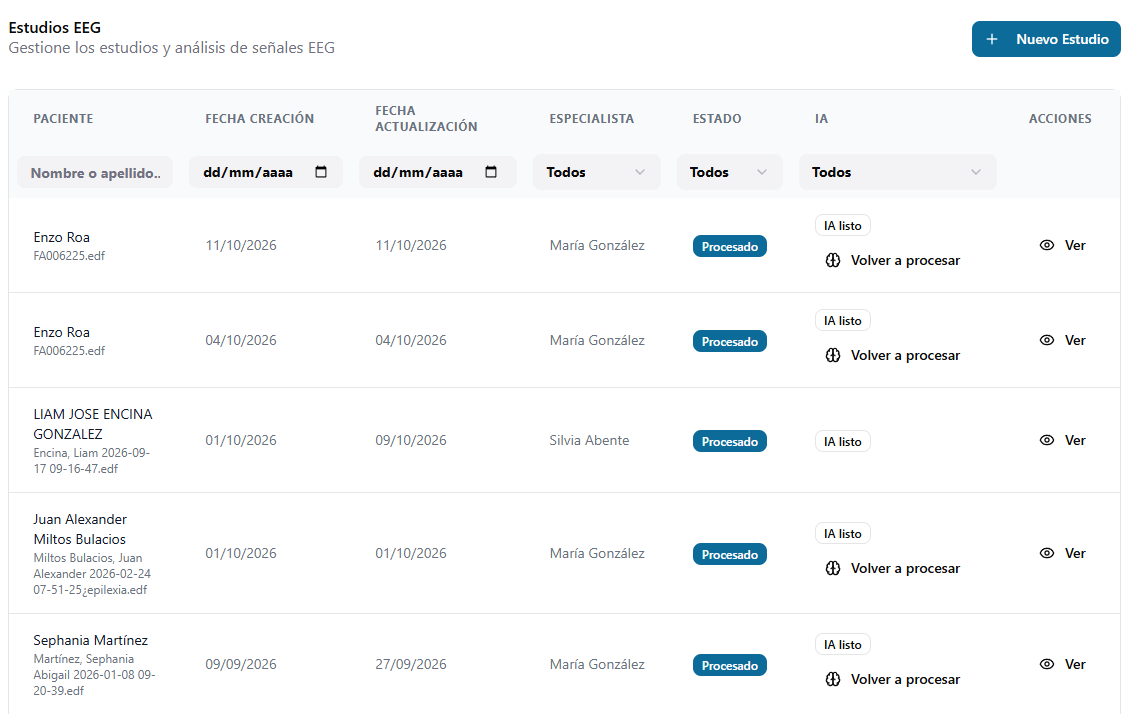
\includegraphics[width=\textwidth]{ThesisFigs/gestion_estudios_eeg.png}
    \caption{Interfaz de gestión de estudios EEG de EpilexIA.}
    \label{fig:gestion-estudios-eeg}
\end{figure}


El registro de un nuevo estudio se realiza mediante un formulario que permite seleccionar al paciente asociado e incorporar el archivo de señales EEG en formato EDF. La interfaz presenta diferencias según el perfil del usuario: en el caso del Técnico, se requiere seleccionar al especialista responsable del estudio, mientras que para el perfil Especialista dicho campo no se muestra. Asimismo, el formulario ofrece la posibilidad de adjuntar un video de monitoreo en formato MP4 o mediante archivos correspondientes a una grabación EZVideo.

Cuando el paciente requerido no se encuentra disponible en
el selector, la aplicación permite registrar uno nuevo sin
abandonar el proceso de creación del estudio. Esta operación
se realiza mediante un formulario que contempla datos de
identificación, información personal y datos de contacto.
De esta manera, el registro de pacientes se integra como
una funcionalidad complementaria a la creación de estudios
EEG, sin constituir un módulo independiente de gestión
de pacientes.

La Figura~\ref{fig:nuevo-estudio-eeg} presenta el formulario de creación de estudios EEG correspondiente al perfil Especialista. En ella se observan el campo de selección del paciente, así como los controles para incorporar el archivo EEG y, opcionalmente, un video de monitoreo.

\begin{figure}[H]
    \centering
    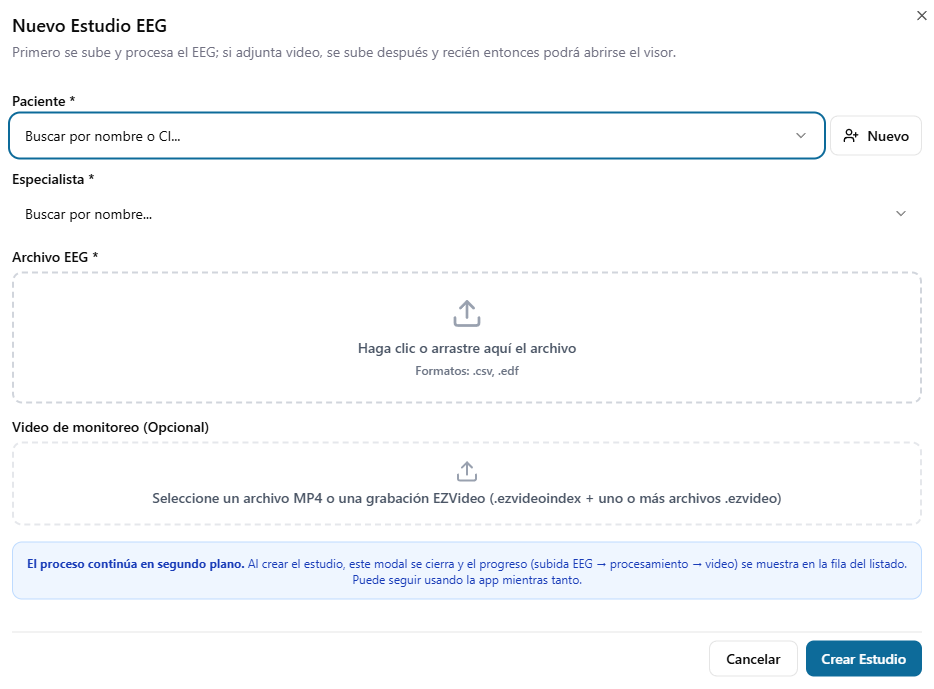
\includegraphics[width=\textwidth]{ThesisFigs/nuevo-estudio-eeg.png}
    \caption{Formulario de creación de estudios EEG correspondiente al perfil Especialista de EpilexIA.}
    \label{fig:nuevo-estudio-eeg}
\end{figure}

La creación del estudio contempla operaciones de carga y
procesamiento de archivos que continúan en segundo plano.
Una vez iniciado el procedimiento, el usuario puede seguir
utilizando la aplicación, mientras que el avance de las
operaciones se presenta en el listado de estudios. Este
mecanismo permite integrar la incorporación de archivos
y su preparación para la visualización posterior.

La organización de las pantallas de estudios también facilita
el acceso a las funcionalidades posteriores del proceso.
Desde un estudio registrado, los usuarios habilitados pueden
acceder a la visualización de señales electroencefalográficas
y a las herramientas de revisión clínica. De esta manera,
el registro inicial de los estudios se integra con las
actividades de análisis y elaboración de informes.

Las operaciones de consulta y actualización se complementan
con controles de búsqueda, acciones contextuales y mensajes
de estado. Estos elementos permiten localizar información,
identificar las operaciones disponibles y conocer el resultado
de las solicitudes realizadas, manteniendo una organización
consistente entre las distintas interfaces de gestión.

En conjunto, las interfaces de administración y gestión de
estudios proporcionan los medios necesarios para organizar
los usuarios del sistema, registrar estudios EEG e incorporar
los archivos utilizados durante la revisión clínica. Su
diseño establece una continuidad entre la administración
de cuentas, la preparación de estudios y el acceso a las
herramientas especializadas de análisis electroencefalográfico.


\subsection{Interfaz de visualización y análisis de señales EEG}

La interfaz de visualización y análisis de señales electroencefalográficas constituye uno de los componentes centrales de EpilexIA. Su diseño está orientado a facilitar la exploración de los registros EEG y proporcionar al especialista herramientas para examinar la actividad eléctrica cerebral, identificar posibles alteraciones y relacionar los hallazgos con la información asociada al estudio.

El acceso al visualizador se realiza desde la interfaz de gestión de estudios, mediante las acciones disponibles para cada registro. Una vez seleccionado un estudio, el sistema presenta las señales electroencefalográficas correspondientes, organizadas por canales y representadas gráficamente en función del tiempo. Esta disposición permite observar simultáneamente diferentes derivaciones y analizar su comportamiento durante el intervalo seleccionado.

La organización del visualizador contempla un área principal destinada a la representación de las señales EEG y un conjunto de controles que permiten modificar las condiciones de visualización. Estos elementos se distribuyen de manera que el usuario pueda realizar ajustes durante la exploración del registro sin abandonar el entorno de análisis.

La Figura~\ref{fig:interfaz-general-eeg} presenta la interfaz general de visualización y análisis de señales EEG de EpilexIA. En ella se observa la distribución del área de representación de las señales, los controles de configuración y navegación temporal, el panel de anomalías y el espacio destinado a la elaboración del informe médico.

\begin{figure}[H]
    \centering
    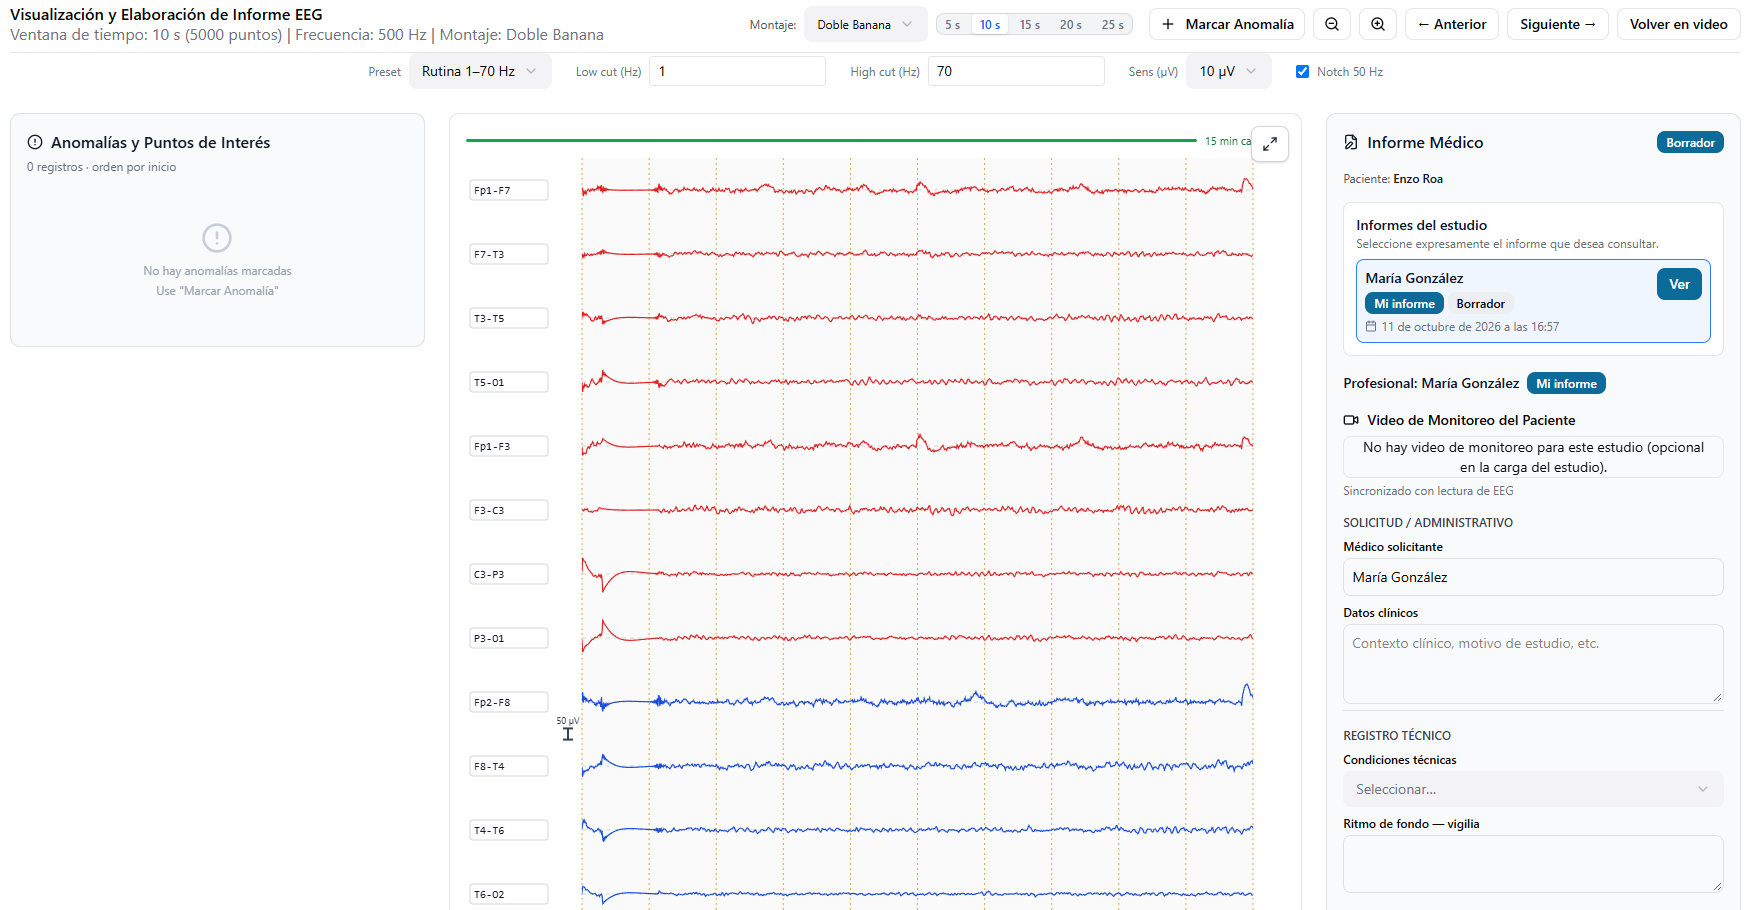
\includegraphics[width=\textwidth]{ThesisFigs/interfaz-general-eeg.png}
    \caption{Interfaz general de visualización y análisis de señales EEG de EpilexIA.}
    \label{fig:interfaz-general-eeg}
\end{figure}

Entre las funcionalidades disponibles se encuentra la navegación temporal, que permite desplazarse a lo largo del registro electroencefalográfico y examinar diferentes intervalos de tiempo. La interfaz incorpora controles para avanzar y retroceder por la señal, así como opciones para ajustar la ventana temporal representada. De esta manera, el especialista puede explorar tanto segmentos específicos como diferentes partes del estudio.

El visualizador también permite seleccionar montajes electroencefalográficos, mediante los cuales se determina la organización de las derivaciones presentadas. Esta funcionalidad facilita la revisión de las señales desde distintas configuraciones de canales, de acuerdo con las necesidades del análisis. Entre las configuraciones contempladas se encuentran los montajes bipolares y referenciales utilizados en la interpretación de registros EEG.

Otro elemento importante corresponde a los controles de filtrado y sensibilidad. Los filtros permiten ajustar la representación de las señales según los parámetros disponibles en la interfaz, mientras que el control de sensibilidad, expresado en microvoltios ($\mu$V), permite modificar la escala vertical de las ondas. Estos ajustes contribuyen a mejorar la observación de determinadas características de la actividad electroencefalográfica, sin modificar el archivo original del estudio.

Como herramienta complementaria, el visualizador incorpora un espectrograma que permite representar la distribución de la actividad de las señales EEG en función del tiempo y la frecuencia. Esta representación proporciona una perspectiva adicional para la exploración del registro electroencefalográfico.

Para ampliar el espacio destinado al análisis, EpilexIA incorpora un modo de pantalla completa. Esta funcionalidad permite visualizar las señales EEG en un área de mayor tamaño, reduciendo la presencia de otros elementos de la interfaz. El usuario puede continuar utilizando los controles de análisis disponibles y regresar posteriormente a la vista habitual.

La Figura~\ref{fig:visualizador-eeg-pantalla-completa} presenta el visualizador EEG en modo de pantalla completa, donde se observan simultáneamente múltiples canales electroencefalográficos, los controles laterales de navegación y el espectrograma ubicado en la parte inferior de la interfaz.

\begin{figure}[H]
    \centering
    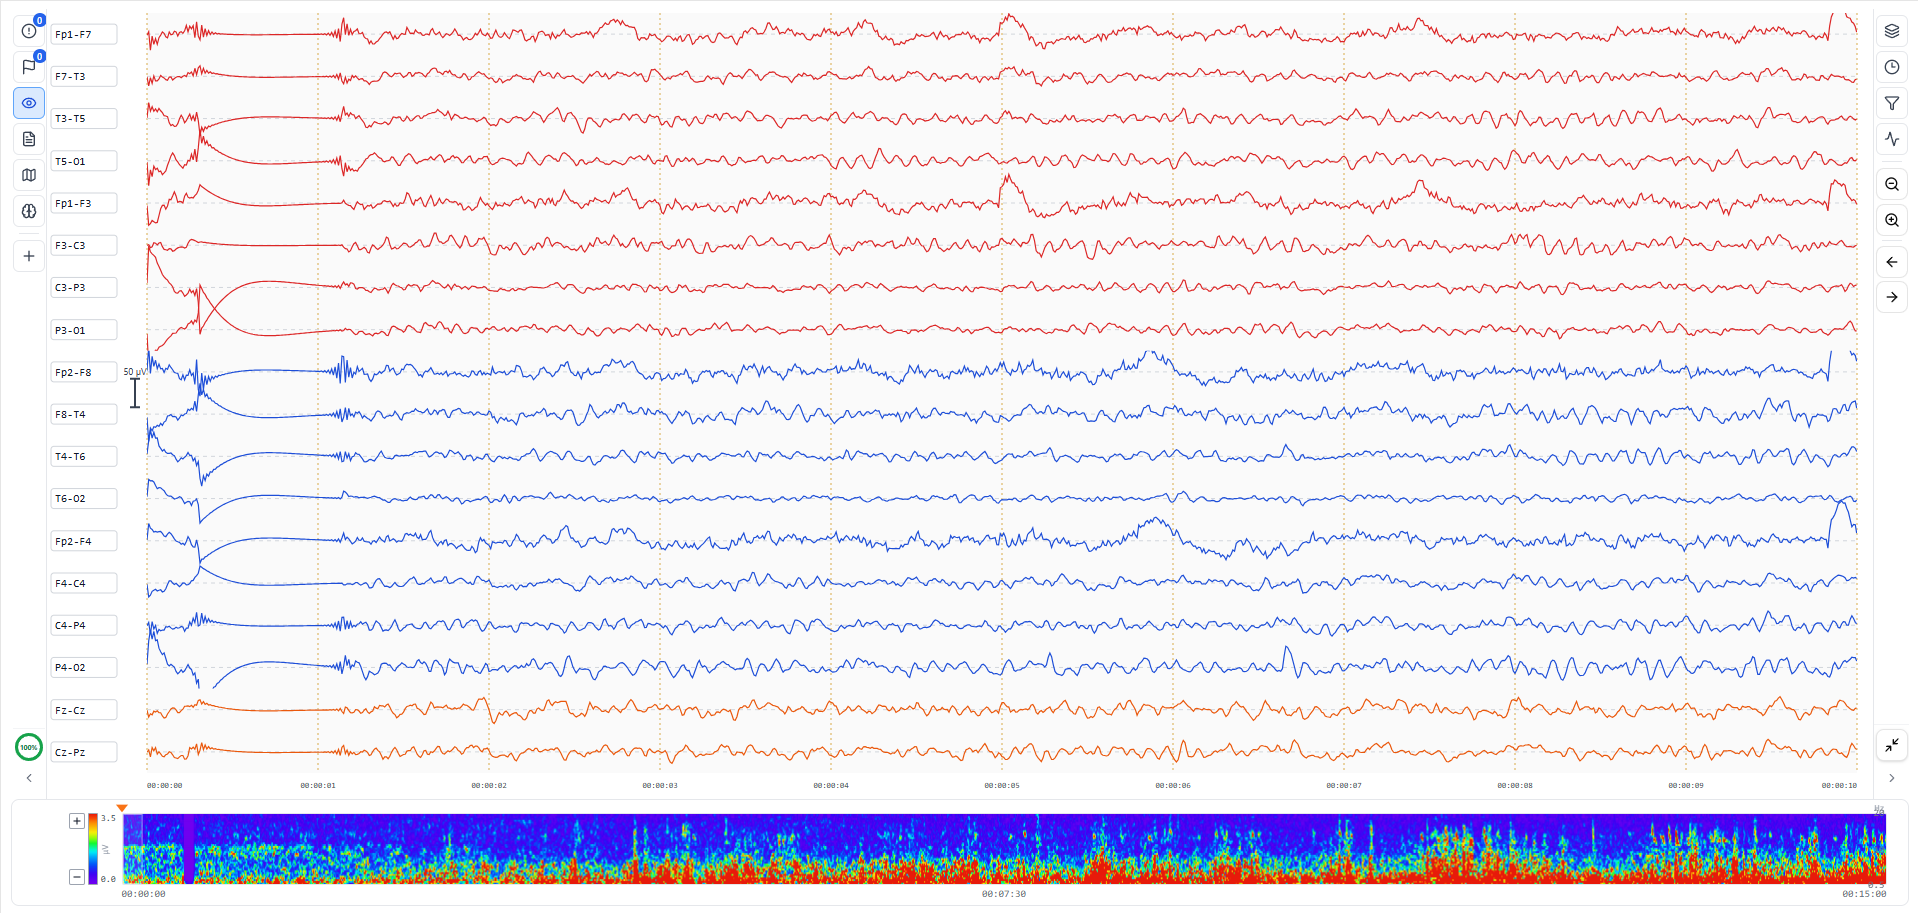
\includegraphics[width=\textwidth]{ThesisFigs/visualizador-eeg-pantalla-completa.png}
    \caption{Visualizador de señales EEG en modo de pantalla completa de EpilexIA.}
    \label{fig:visualizador-eeg-pantalla-completa}
\end{figure}

La interfaz también contempla la presentación de información relacionada con anomalías y eventos asociados al estudio. Estos elementos permiten vincular determinados intervalos del registro con observaciones realizadas durante su revisión. Asimismo, cuando existen resultados de procesamiento mediante inteligencia artificial, el especialista puede utilizarlos como información complementaria para orientar la exploración de segmentos de interés.

La visualización de las señales se integra con las demás funcionalidades de revisión clínica de EpilexIA. De esta manera, el especialista puede examinar los registros electroencefalográficos y relacionar los hallazgos observados con las actividades de documentación y elaboración de informes médicos correspondientes al estudio.

En conjunto, el diseño del visualizador EEG reúne herramientas de navegación, configuración y exploración de señales dentro de una misma interfaz. Su organización busca facilitar el análisis de registros electroencefalográficos y proporcionar un entorno de trabajo que apoye la revisión clínica realizada por el especialista.

\subsection[Interfaces de revisión clínica y elaboración de informes médicos]
{Interfaces de revisión clínica y elaboración de\\informes médicos}

Las interfaces de revisión clínica y elaboración de informes médicos de EpilexIA están orientadas a facilitar la documentación de los hallazgos identificados durante el análisis de los estudios electroencefalográficos. Estas funcionalidades permiten al especialista relacionar las observaciones realizadas sobre las señales EEG con la información clínica correspondiente y organizar los resultados de su evaluación dentro de un mismo entorno de trabajo.

La revisión clínica se desarrolla a partir de los estudios registrados en el sistema. Una vez que el especialista accede a un estudio, dispone de herramientas para examinar las señales electroencefalográficas, identificar segmentos de interés y registrar observaciones relacionadas con posibles alteraciones. Estas operaciones se integran con el visualizador EEG, permitiendo mantener una relación entre los hallazgos documentados y los intervalos temporales del registro.

Entre las funcionalidades disponibles se encuentra el registro de anomalías y eventos asociados al estudio. Estas herramientas permiten documentar situaciones identificadas durante la exploración de las señales y vincularlas con determinados segmentos del registro electroencefalográfico. La información registrada constituye un recurso de apoyo para la revisión posterior y la elaboración del informe médico.


Cuando un estudio dispone de resultados de inteligencia artificial previamente almacenados, la interfaz permite consultar los intervalos señalados en dichos registros. Estos resultados se presentan como información complementaria para orientar la revisión del especialista, quien conserva la responsabilidad de examinar las señales y determinar la relevancia clínica de los hallazgos. De esta manera, el sistema integra el apoyo automatizado sin sustituir la interpretación realizada por el profesional.


La Figura~\ref{fig:panel-anomalias-ia} presenta el panel de anomalías y puntos de interés de EpilexIA, en el que se observan los intervalos identificados mediante inteligencia artificial, sus respectivas referencias temporales y los controles disponibles para su consulta. Asimismo, la interfaz incorpora filtros que permiten distinguir entre los registros generados automáticamente y aquellos incorporados de forma manual.

\begin{figure}[H]
    \centering
    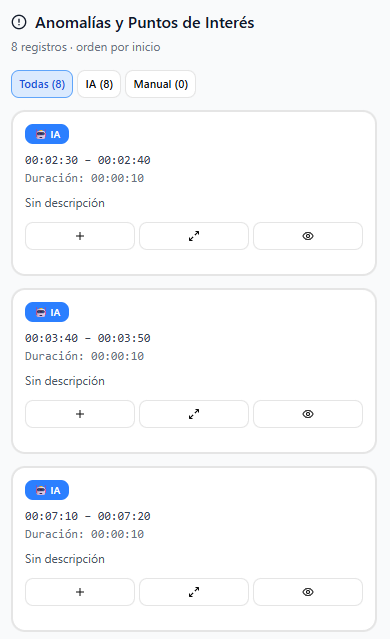
\includegraphics[width=0.55\textwidth]{ThesisFigs/panel_anomalias_ia.png}
    \caption{Panel de anomalías y puntos de interés de EpilexIA con resultados de inteligencia artificial.}
    \label{fig:panel-anomalias-ia}
\end{figure}

La elaboración de informes médicos constituye otra funcionalidad central de este entorno. EpilexIA incorpora una interfaz que permite registrar y actualizar la información correspondiente a la evaluación clínica del estudio. Los formularios se organizan mediante secciones destinadas a documentar los antecedentes y datos clínicos pertinentes, las observaciones sobre el registro electroencefalográfico y las conclusiones del especialista.

La interfaz de informes se encuentra vinculada al estudio EEG correspondiente, lo que facilita la consulta de las señales durante la elaboración del documento. Esta integración permite que el especialista mantenga disponibles los elementos necesarios para relacionar las observaciones realizadas con la información incorporada al informe médico.


El sistema contempla la participación de diferentes Especialistas autorizados en la revisión de un mismo estudio. Cada Especialista puede elaborar un único informe médico propio por estudio, manteniendo diferenciados los registros correspondientes a cada autor. Esta organización permite conservar la individualidad de las evaluaciones y garantiza que ningún Especialista pueda modificar el contenido de un informe perteneciente a otro profesional.


Los informes médicos disponen de estados que permiten distinguir aquellos que se encuentran en Borrador de los que han sido Cerrados. Durante la etapa de borrador, el especialista puede continuar registrando y actualizando la información correspondiente. Una vez cerrado el informe, se aplican las restricciones establecidas por el sistema para impedir modificaciones posteriores.

La presentación de los informes incorpora controles para seleccionar los documentos asociados al estudio y consultar su contenido, de acuerdo con los permisos del usuario. Asimismo, las acciones de creación, edición y cierre se encuentran diferenciadas según el estado del informe y las autorizaciones correspondientes al especialista.

La Figura~\ref{fig:interfaz-informe-medico} presenta la interfaz de elaboración de informes médicos de EpilexIA. En ella se observan las secciones destinadas al registro de información administrativa, datos clínicos, condiciones técnicas, hallazgos ictales e interictales, conclusiones y observaciones. Asimismo, se muestran los controles disponibles para guardar el informe, consultar su vista previa y proceder a su cierre.


\begin{figure}[H]
    \centering

    \begin{minipage}[t]{0.46\textwidth}
        \vspace{0pt}
        \centering
        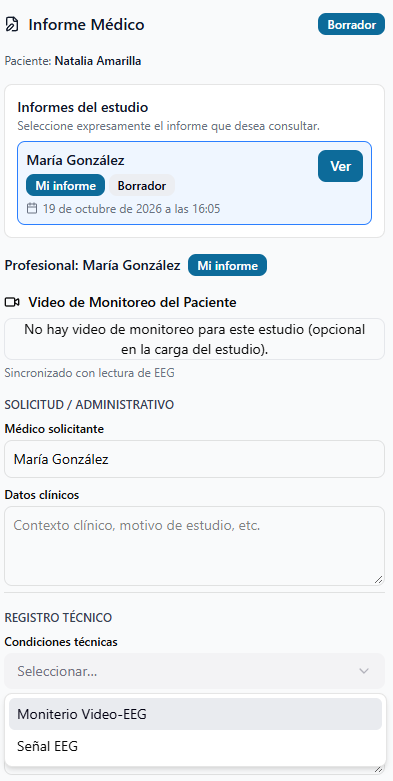
\includegraphics[width=\linewidth]{ThesisFigs/informe_medico_superior.png}
    \end{minipage}
    \hfill
    \begin{minipage}[t]{0.46\textwidth}
        \vspace{0pt}
        \centering
        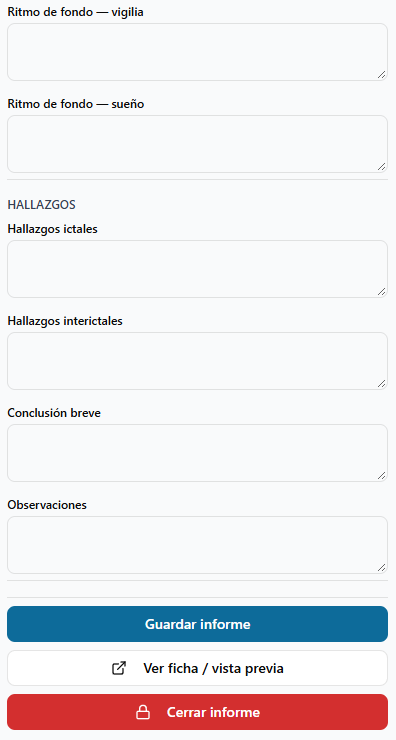
\includegraphics[width=\linewidth]{ThesisFigs/informe_medico_inferior.png}
    \end{minipage}

    \caption{Interfaz de elaboración de informes médicos de EpilexIA.}
    \label{fig:interfaz-informe-medico}
\end{figure}

En conjunto, las interfaces de revisión clínica y elaboración de informes médicos permiten integrar la identificación de hallazgos, el registro de anomalías y eventos, la consulta de resultados de inteligencia artificial y la documentación de las evaluaciones profesionales. Su diseño busca proporcionar un entorno de trabajo organizado que facilite la continuidad entre el análisis de las señales EEG y la elaboración de los informes médicos asociados a cada estudio.

\clearpage
\lhead{\emph{Anexo B. Implementación del sistema}}
\chapter{Implementación del sistema}
\label{cap:implementacion-sistema}

\section{Introducción}
\label{introduccion}

En este capítulo se describe el proceso de implementación del sistema
EpilexIA, desarrollado como una solución informática de apoyo al
análisis de estudios electroencefalográficos y al proceso de diagnóstico
de la epilepsia, mediante la gestión de estudios EEG,
la visualización de señales EEG, la integración de registros de video
y la utilización de técnicas de inteligencia artificial.

La implementación se llevó a cabo a partir de los requerimientos
funcionales y no funcionales, así como de las decisiones arquitectónicas
y de diseño presentadas en el capítulo anterior. Para ello, se utilizaron
tecnologías de código abierto y una organización modular que permite
separar las responsabilidades de la interfaz de usuario, los servicios
de aplicación, la persistencia de datos y los componentes asociados
al procesamiento mediante inteligencia artificial.

El desarrollo comprendió la construcción e integración de las
funcionalidades necesarias para el registro y seguimiento de estudios
EEG, la incorporación y preparación de archivos, la visualización
y análisis de señales electroencefalográficas, la identificación
y gestión de anomalías y eventos, y la elaboración de informes
médicos. Asimismo, se implementaron mecanismos de autenticación,
autorización y auditoría para controlar el acceso a los recursos
y registrar las operaciones correspondientes.

En los siguientes apartados se presentan las tecnologías y herramientas
empleadas, la implementación de los principales componentes del sistema
y los mecanismos utilizados para su integración y despliegue.
La descripción se centra en las decisiones técnicas y en las soluciones
adoptadas durante el desarrollo, con el propósito de mostrar cómo
los elementos definidos en la etapa de diseño fueron implementados
e integrados en el sistema desarrollado.


\section{Entorno de desarrollo y tecnologías utilizadas}
\label{entorno-desarrollo-tecnologias-utilizadas}

La implementación de EpilexIA se realizó mediante un conjunto de tecnologías y herramientas orientadas al desarrollo de aplicaciones web, la gestión de información clínica y el procesamiento de señales electroencefalográficas mediante inteligencia artificial. La selección de estos componentes permitió organizar el sistema en módulos con responsabilidades diferenciadas, facilitando su desarrollo, integración y mantenimiento.

El entorno tecnológico comprende herramientas de gestión de código fuente, construcción de aplicaciones, administración de dependencias y ejecución de pruebas, así como \textit{frameworks}, bibliotecas y servicios utilizados para implementar los distintos componentes del sistema. En los siguientes apartados se describen las principales herramientas empleadas y su función dentro de la solución desarrollada.

\subsection{Herramientas y entorno de desarrollo}
\label{herramientas-entorno-desarrollo}

El desarrollo de EpilexIA se organizó mediante cinco repositorios de código fuente, correspondientes a la interfaz web, los servicios de aplicación, la base de datos clínica, la API de inteligencia artificial y el motor de procesamiento. Esta separación permitió administrar de manera diferenciada los componentes del sistema, sus dependencias y sus configuraciones de ejecución.

Para la gestión del código fuente se utilizó Git, herramienta de control de versiones que permite registrar los cambios realizados durante el desarrollo y mantener un historial de las modificaciones. La organización en repositorios independientes facilita el seguimiento de los componentes y la incorporación de nuevas funcionalidades.

La administración de dependencias y la construcción de las aplicaciones se realizaron mediante herramientas específicas para cada entorno tecnológico. En el \textit{frontend} se utilizó npm para gestionar las dependencias de JavaScript y TypeScript, junto con Vite para ejecutar el servidor de desarrollo y generar los archivos de distribución de la aplicación web. En el \textit{backend} se empleó Maven para administrar las dependencias de Java, ejecutar las tareas de construcción y generar el archivo WAR destinado al servidor de aplicaciones. Por su parte, los componentes desarrollados en Python utilizan archivos de requisitos y el gestor pip para definir e instalar sus dependencias.

Para la verificación del \textit{software}, los repositorios incorporan herramientas de pruebas adaptadas a sus respectivas tecnologías. El \textit{frontend} dispone de Vitest y Testing Library para realizar pruebas sobre componentes y funcionalidades de la interfaz. El \textit{backend} utiliza las herramientas de pruebas de Spring Boot, junto con JUnit, Mockito y Spring Security Test. Los componentes desarrollados en Python incluyen pruebas implementadas mediante el módulo \texttt{unittest}.

Asimismo, se utilizaron mecanismos de configuración específicos para los distintos componentes. El \textit{frontend} emplea variables de entorno gestionadas durante su construcción, mientras que los servicios del \textit{backend}, la API de inteligencia artificial y el motor de procesamiento disponen de parámetros de configuración para establecer conexiones, rutas de archivos y condiciones de ejecución.

Estas herramientas proporcionaron una base de trabajo para desarrollar y mantener los distintos componentes de EpilexIA, conservando la separación entre sus entornos tecnológicos y permitiendo realizar tareas de construcción, configuración y verificación de manera independiente.


Además del código fuente, cada repositorio contiene los archivos de contexto utilizados por los asistentes de inteligencia artificial (\texttt{CLAUDE.md}, \texttt{AGENTS.md} y las reglas de Cursor) y una carpeta de documentación con los planes y análisis elaborados durante el desarrollo.
El repositorio del \textit{backend} incluye además la especificación general del sistema.
La forma en que estos elementos se utilizaron se describe en el capítulo de metodología del libro.

\subsection{Tecnologías utilizadas}

La implementación de EpilexIA comprende diferentes tecnologías de
programación, \textit{framework}s y bibliotecas, seleccionadas de acuerdo con
las responsabilidades de cada componente del sistema. Esta organización
permite utilizar herramientas especializadas para la construcción de
la interfaz web, la ejecución de la lógica de negocio, la persistencia
de información y el procesamiento de señales electroencefalográficas
mediante inteligencia artificial.

La interfaz web se desarrolló con React, una biblioteca de JavaScript
orientada a la construcción de interfaces mediante componentes
reutilizables. Para su implementación se utilizó TypeScript, que
incorpora tipado estático al desarrollo de aplicaciones basadas en
JavaScript, junto con Vite como herramienta de desarrollo y
construcción. La navegación entre las diferentes secciones se
implementó mediante React Router, mientras que la comunicación con
los servicios del \textit{backend} se realiza utilizando la API nativa Fetch.

El \textit{backend} se implementó mediante Java 21 y Spring Boot, utilizando
Spring Web MVC para la exposición de servicios REST. La persistencia
de información se gestiona mediante Spring Data JPA e Hibernate,
mientras que Spring Security proporciona los mecanismos de
autenticación y autorización. La aplicación se empaqueta en formato
WAR para su ejecución sobre el servidor de aplicaciones WildFly.

Para el almacenamiento de la información clínica se utiliza
PostgreSQL 17, un sistema gestor de bases de datos relacional. Su
implementación contempla estructuras para almacenar pacientes,
estudios electroencefalográficos, usuarios, informes médicos,
anomalías y otros registros asociados al funcionamiento de EpilexIA.

El subsistema de inteligencia artificial se implementó mediante
Python y se encuentra organizado en dos componentes diferenciados.
El primero corresponde a una API desarrollada con FastAPI, encargada de recibir y gestionar las solicitudes relacionadas con el procesamiento de señales EEG y facilitar la comunicación con los servicios asociados. El segundo corresponde a un motor de procesamiento independiente, responsable de ejecutar las tareas de análisis de las señales electroencefalográficas. Ambos componentes utilizan una instancia PostgreSQL destinada a almacenar información relacionada con las ejecuciones y los resultados del procesamiento.


Para el tratamiento de señales electroencefalográficas se utilizan
bibliotecas científicas como MNE-Python, NumPy, SciPy y pandas.
Asimismo, se emplea joblib para cargar modelos previamente
entrenados y scikit-learn como dependencia necesaria para su
ejecución. Estas herramientas permiten desarrollar las operaciones
de lectura, transformación y procesamiento de datos requeridas
por el subsistema de inteligencia artificial.

Las tecnologías utilizadas en el desarrollo de EpilexIA
fueron seleccionadas considerando los requerimientos
funcionales del sistema, la integración entre sus
componentes y la disponibilidad de herramientas
de código abierto.

El Cuadro~\ref{tab:comparacion_tecnologias} presenta
una comparación cualitativa de tecnologías alternativas
aplicables a los distintos componentes de la arquitectura,
junto con los principales criterios que fundamentan
las elecciones realizadas.

\begin{table}[htbp]
\centering
\caption{Comparación de tecnologías para el desarrollo de EpilexIA.}
\label{tab:comparacion_tecnologias}
\scriptsize
\setlength{\tabcolsep}{3pt}
\renewcommand{\arraystretch}{1.15}

\begin{tabular}{|
>{\raggedright\arraybackslash}p{2.1cm}|
>{\raggedright\arraybackslash}p{2.4cm}|
>{\raggedright\arraybackslash}p{2.8cm}|
>{\raggedright\arraybackslash}p{3.6cm}|}
\hline
\textbf{Componente} &
\textbf{Selección} &
\textbf{Alternativas} &
\textbf{Criterio de selección} \\
\hline

\textit{Frontend} &
React &
Angular, Vue.js &
Componentes reutilizables y visualización interactiva. \\
\hline

\textit{Backend} &
Spring Boot &
Django, ASP.NET Core &
Servicios REST, modularidad e integración con Java. \\
\hline

Base de datos &
PostgreSQL &
MySQL, MariaDB &
Integridad relacional, transacciones y persistencia de datos. \\
\hline

API de IA &
FastAPI &
Flask, Django REST Framework &
Integración con Python y exposición de servicios REST. \\
\hline

Motor de IA &
Python &
Java, R &
Bibliotecas científicas y herramientas de aprendizaje automático. \\
\hline

Contenedores &
Docker &
Podman &
Aislamiento de servicios y despliegue reproducible. \\
\hline

\end{tabular}
\end{table}

A partir de esta comparación, se adoptó una
arquitectura que combina React para la interfaz
web, Spring Boot para los servicios de aplicación,
PostgreSQL para la persistencia de información
y Python con FastAPI para los componentes de
inteligencia artificial. Docker permite organizar
y desplegar los servicios en contenedores.

Las tecnologías y versiones concretas utilizadas
en la implementación se presentan en el
Cuadro~\ref{tab:tecnologias_epilexia}.

\begingroup
\small
\setlength{\tabcolsep}{3pt}
\renewcommand{\arraystretch}{1.08}
\setlength{\LTleft}{0pt}
\setlength{\LTright}{0pt}

\begin{longtable}{|
p{0.18\dimexpr\textwidth-8\tabcolsep-5\arrayrulewidth\relax}|
p{0.19\dimexpr\textwidth-8\tabcolsep-5\arrayrulewidth\relax}|
p{0.18\dimexpr\textwidth-8\tabcolsep-5\arrayrulewidth\relax}|
p{0.45\dimexpr\textwidth-8\tabcolsep-5\arrayrulewidth\relax}|}

\caption[Principales tecnologías utilizadas en EpilexIA]%
{Tecnologías utilizadas en EpilexIA.}
\label{tab:tecnologias_epilexia}\\
\hline
\textbf{Componente} &
\textbf{Tecnología} &
\textbf{Versión} &
\textbf{Función principal} \\
\hline
\endfirsthead

\multicolumn{4}{c}{\textit{Continuación del Cuadro~\ref{tab:tecnologias_epilexia}}}\\
\hline
\textbf{Componente} &
\textbf{Tecnología} &
\textbf{Versión} &
\textbf{Función principal} \\
\hline
\endhead

\textit{Frontend} & React & 18.3.1 &
Construcción de la interfaz web \\
\hline
\textit{Frontend} & TypeScript & --- &
Desarrollo tipado de la interfaz \\
\hline
\textit{Frontend} & Vite & 6.3.5 &
Desarrollo y construcción \\
\hline
\textit{Backend} & Java & 21 &
Implementación de la lógica de negocio \\
\hline
\textit{Backend} & Spring Boot & 3.5.11 &
Desarrollo de servicios de aplicación \\
\hline
\textit{Backend} & WildFly & 39.0.0.Final &
Ejecución de la aplicación \textit{backend} \\
\hline
Base de datos clínica & PostgreSQL & 17 &
Persistencia de información clínica \\
\hline
API de IA & Python & 3.13 &
Implementación de servicios de IA \\
\hline
API de IA & FastAPI & 0.115.6 &
Exposición de servicios de integración \\
\hline
Base de datos de IA & PostgreSQL & 16 &
Persistencia de ejecuciones y resultados \\
\hline
Motor de IA & Python & 3.13 &
Ejecución del procesamiento EEG \\
\hline
Motor de IA & MNE-Python & $\geq$\,\texttt{1.8.0} &
Lectura y procesamiento de señales EEG \\
\hline
Motor de IA & joblib & $\geq$\,\texttt{1.3.0} &
Carga de modelos serializados \\
\hline
Motor de IA & scikit-learn & 1.8.0 &
Ejecución del modelo entrenado \\
\hline

\end{longtable}
\endgroup

Las versiones indicadas corresponden a las dependencias y
configuraciones de los repositorios del proyecto.
En los casos en que se especifican rangos de versiones, la
versión efectiva depende de las dependencias instaladas durante
la construcción de cada componente. Para TypeScript, el proyecto no fija una
versión propia: la transpilación la realiza Vite.

La combinación de estas tecnologías proporciona los recursos
necesarios para implementar las funcionalidades de EpilexIA,
manteniendo diferenciadas las responsabilidades de la interfaz
web, los servicios de aplicación, las bases de datos y el
procesamiento mediante inteligencia artificial.


\subsection{Herramientas de integración y despliegue}

La integración de los componentes de EpilexIA se realiza mediante
herramientas de contenedorización y servicios de ejecución que
permiten configurar los distintos entornos tecnológicos del
sistema. Estas herramientas facilitan la construcción de las
aplicaciones, la administración de sus dependencias y la
comunicación entre los servicios que conforman la solución.

Para la contenedorización se utiliza Docker, que permite
empaquetar las aplicaciones junto con sus dependencias y
configuraciones de ejecución. Cada uno de los componentes
principales dispone de archivos de configuración que establecen
las instrucciones necesarias para construir sus respectivas
imágenes y definir las condiciones de funcionamiento dentro
de los contenedores.

La coordinación de los servicios se realiza mediante Docker
Compose, que permite definir y administrar conjuntos de
contenedores a través de archivos de configuración. En EpilexIA,
estos archivos contemplan servicios para la interfaz web, el
\textit{backend}, las bases de datos y los componentes de inteligencia
artificial. Asimismo, permiten establecer redes de comunicación,
volúmenes de almacenamiento y parámetros de configuración
necesarios para la integración del sistema.

La publicación de la interfaz web se realiza mediante Nginx,
utilizado para servir los archivos estáticos generados durante
la construcción de la aplicación React. Su configuración
también contempla el encaminamiento de solicitudes hacia los
servicios del \textit{backend}, permitiendo que la interfaz acceda a
las funcionalidades expuestas por la aplicación.

El \textit{backend} se ejecuta sobre WildFly, un servidor de aplicaciones
compatible con el entorno Java utilizado en EpilexIA. La
aplicación desarrollada con Spring Boot se empaqueta en formato
WAR y se incorpora al servidor para exponer los servicios REST
responsables de las operaciones de negocio y del acceso a la
información clínica.

Por su parte, la API de inteligencia artificial utiliza Uvicorn
como servidor ASGI para ejecutar la aplicación desarrollada con
FastAPI. Este componente recibe las solicitudes de procesamiento
procedentes del \textit{backend} y coordina las operaciones asociadas a
las ejecuciones de inteligencia artificial.

El motor de inteligencia artificial se ejecuta como un proceso
independiente, sin exponer un servicio HTTP propio. La API registra las solicitudes en la base de datos PostgreSQL destinada al
subsistema de inteligencia artificial, mientras que el motor
consulta y procesa las tareas pendientes. Este mecanismo permite desacoplar la recepción de solicitudes de la ejecución
del procesamiento de señales EEG.

La integración también contempla el uso de volúmenes de
almacenamiento compartidos para facilitar el acceso a los
archivos electroencefalográficos requeridos durante el
procesamiento. Asimismo, los servicios utilizan parámetros
de configuración para establecer sus conexiones y rutas de
acceso, evitando incorporar estos valores directamente en
el código de las aplicaciones.

Las configuraciones disponibles permiten establecer entornos de ejecución locales y un despliegue integrado con servicios y redes diferenciadas, utilizado en el entorno en la nube que se describe en la Sección~\ref{subsec:despliegue-nube}.

En conjunto, Docker, Docker Compose, Nginx, WildFly y Uvicorn
proporcionan los mecanismos necesarios para ejecutar e integrar
los componentes de EpilexIA, manteniendo diferenciadas sus
responsabilidades y facilitando la configuración de los
servicios que conforman el sistema.


\section{Implementación de la base de datos}

La persistencia de información en EpilexIA se implementó mediante
dos bases de datos PostgreSQL independientes, destinadas a la
gestión de la información clínica y al almacenamiento de los
datos asociados al procesamiento mediante inteligencia
artificial. Esta separación permite organizar los registros
de acuerdo con las responsabilidades de los componentes que
integran el sistema.

La base de datos clínica almacena la información relacionada
con usuarios, pacientes, estudios electroencefalográficos,
archivos asociados, anomalías, informes médicos y registros
de auditoría. Su estructura se implementó mediante \textit{scripts}
SQL y se integra con el \textit{backend} desarrollado en Spring Boot
a través de Spring Data JPA e Hibernate.

Por otra parte, el subsistema de inteligencia artificial
dispone de una base de datos destinada a registrar las
solicitudes de procesamiento, sus estados de ejecución,
los resultados obtenidos y otros datos asociados al análisis
de señales EEG. La persistencia de este componente se
implementó mediante SQLAlchemy, mientras que la evolución
de su esquema se administra principalmente mediante Alembic.

El almacenamiento de los archivos electroencefalográficos
y de video se realiza fuera de las bases de datos, mediante
directorios y volúmenes de almacenamiento. PostgreSQL conserva
las referencias y los metadatos necesarios para relacionar
estos recursos con los estudios correspondientes.

En los siguientes apartados se describe la arquitectura de
persistencia, la implementación del esquema clínico, los
mecanismos de almacenamiento de archivos y la gestión de
datos del subsistema de inteligencia artificial. Se
presentan las principales decisiones técnicas adoptadas,
sin reiterar el modelo conceptual y las relaciones ya
desarrolladas en el capítulo de diseño.


\subsection{Arquitectura de persistencia}

La arquitectura de persistencia de EpilexIA se organiza mediante
dos bases de datos PostgreSQL independientes y un sistema de
almacenamiento de archivos. Esta distribución permite mantener
separada la información clínica de los registros utilizados
durante el procesamiento mediante inteligencia artificial,
asignando responsabilidades específicas a cada componente.

La base de datos clínica, implementada sobre PostgreSQL 17,
es utilizada por el \textit{backend} desarrollado con Spring Boot.
A través de Spring Data JPA e Hibernate, el \textit{backend} realiza
las operaciones de persistencia y consulta de información
relacionada con usuarios, pacientes, estudios
electroencefalográficos, informes médicos, anomalías y
registros de auditoría. Las operaciones se encuentran
sujetas a las reglas de negocio y a los mecanismos de
autorización establecidos en los servicios de aplicación.

Por su parte, el subsistema de inteligencia artificial
utiliza una instancia PostgreSQL 16, a la que acceden
la API desarrollada con FastAPI y el motor de procesamiento.
La API emplea SQLAlchemy para administrar los registros
asociados a las solicitudes de análisis, sus estados de
ejecución y los resultados generados. El motor consulta
la información necesaria para ejecutar las tareas y
persistir los resultados del procesamiento.


Dado que las bases de datos clínica y de inteligencia
artificial corresponden a instancias PostgreSQL
independientes, no se establecen relaciones de integridad
referencial directas entre sus estructuras. La asociación
de la información se realiza mediante identificadores
de estudios y referencias lógicas utilizadas por los
componentes de aplicación. De esta manera, cada instancia
mantiene su propio esquema y sus mecanismos de persistencia.


El almacenamiento de archivos EEG y de video se realiza
en directorios del sistema de archivos, que pueden
incorporarse a los contenedores mediante volúmenes de
almacenamiento. La base de datos clínica conserva los
metadatos y las referencias correspondientes, permitiendo
vincular los recursos almacenados con los estudios
electroencefalográficos.

Esta arquitectura diferencia tres responsabilidades
principales: la persistencia de información clínica,
el registro de las ejecuciones y resultados de
inteligencia artificial, y el almacenamiento físico
de archivos asociados a los estudios. Su integración
permite que los componentes del sistema accedan a la
información necesaria para desarrollar sus funciones,
sin concentrar todos los datos en una única base
de datos.

La Figura~\ref{fig:arquitectura-persistencia}
representa la distribución de los componentes
responsables de la persistencia de información
en EpilexIA. Se distinguen las dos instancias
PostgreSQL y el almacenamiento externo de archivos
asociados a los estudios electroencefalográficos.


\begin{figure}[!htbp]
\centering

\begin{tikzpicture}[
    >=Latex,
    font=\small,
    componente/.style={
        draw,
        rounded corners=2pt,
        align=center,
        minimum height=0.9cm,
        text width=3.2cm
    },
    bd/.style={
        componente,
        fill=gray!10
    },
    conexion/.style={
        <->,
        thick
    }
]

% Subsistema clínico
\node[componente] (backend) at (0,4)
    {\textit{Backend} Spring Boot\\
     \footnotesize JPA / Hibernate};

\node[bd] (clinica) at (-2.4,2)
    {PostgreSQL 17\\
     \footnotesize Datos clínicos};

\node[componente] (archivos) at (2.4,2)
    {Sistema de archivos\\
     \footnotesize EEG y video};

% Subsistema de inteligencia artificial
\node[componente] (api) at (-2.4,-0.5)
    {API FastAPI\\
     \footnotesize SQLAlchemy};

\node[componente] (motor) at (2.4,-0.5)
    {Motor de IA\\
     \footnotesize Procesamiento EEG};

\node[bd] (bdia) at (0,-2.5)
    {PostgreSQL 16\\
     \footnotesize Ejecuciones y resultados};

% Conexiones clínicas
\draw[conexion] (backend) -- (clinica);
\draw[conexion] (backend) -- (archivos);

% Comunicación entre backend y API
\draw[->, thick, dashed]
    (backend.west)
    -- ++(-3.2,0)
    |- (api.west);

% Conexiones del subsistema de IA
\draw[conexion] (api) -- (bdia);
\draw[conexion] (motor) -- (bdia);

% Acceso del motor a los archivos EEG
\draw[->, thick, dashed]
    (archivos.south)
    -- (motor.north);

\end{tikzpicture}

\caption{Arquitectura de persistencia de EpilexIA.}
\label{fig:arquitectura-persistencia}

\end{figure}

\FloatBarrier

\subsection{Implementación de la base de datos clínica}

La base de datos clínica de EpilexIA se implementó utilizando
PostgreSQL 17, mediante un esquema relacional destinado a
almacenar y organizar la información necesaria para el
funcionamiento del sistema. Su estructura comprende tablas
relacionadas con usuarios, roles, permisos, pacientes,
estudios electroencefalográficos, archivos asociados,
anomalías, eventos, informes médicos y registros de
auditoría.

La definición inicial de las estructuras se realizó
mediante \textit{scripts} SQL que establecen las tablas, los tipos
de datos, las claves primarias y foráneas, así como las
restricciones necesarias para mantener la integridad de
los registros. La implementación también contempla
índices y valores predeterminados que contribuyen a la
organización y recuperación de la información almacenada.

Entre las relaciones principales se encuentra la
asociación de los estudios electroencefalográficos
con los pacientes registrados. Cada estudio conserva
la referencia al paciente correspondiente y al
especialista asociado, permitiendo identificar la
información clínica relacionada con su realización
y posterior revisión.

Los archivos vinculados a los estudios se representan
mediante registros que almacenan sus metadatos y
referencias de ubicación. Esta organización permite
mantener la relación entre los estudios y los recursos
electroencefalográficos o audiovisuales, sin incorporar
los archivos binarios directamente en las tablas de
la base de datos.

La persistencia de los informes médicos se organiza
mediante estructuras que permiten asociar diferentes
informes a un mismo estudio, conservando la identificación
del especialista responsable de cada uno. Asimismo,
se implementaron relaciones para registrar segmentos
y otros datos vinculados con el contenido de los
informes, de acuerdo con las reglas de negocio
establecidas en el sistema.

La base de datos también incorpora estructuras para
almacenar anomalías y eventos identificados durante
la revisión de señales EEG. Estos registros permiten
vincular los hallazgos con los estudios correspondientes
y conservar información relacionada con su ubicación
temporal y sus características.

Para el acceso a la información se utiliza Spring Data
JPA junto con Hibernate, integrados en el \textit{backend}
desarrollado con Spring Boot. Las entidades Java
representan las estructuras persistentes del sistema,
mientras que los repositorios proporcionan las
operaciones de consulta y actualización requeridas
por los servicios de aplicación.

La consistencia de los datos se controla mediante
las restricciones definidas en PostgreSQL y las
validaciones implementadas en el \textit{backend}. De esta
manera, las reglas de integridad referencial se
complementan con las comprobaciones realizadas
durante la ejecución de las operaciones de negocio.

La creación inicial de la base de datos clínica se
realiza mediante \textit{scripts} SQL, mientras que las
modificaciones posteriores se incorporan mediante
\textit{scripts} de actualización específicos. Este mecanismo
permite introducir cambios en las estructuras
persistentes y en los datos de configuración
necesarios para la evolución del sistema.

Por último, se implementó una estructura de auditoría
destinada a conservar registros de las operaciones
de negocio catalogadas para su seguimiento. Estos
registros incluyen información descriptiva del
actor y su rol al momento de registrar la operación,
además del tipo de evento y otros datos asociados,
facilitando la consulta histórica de las actividades
realizadas en EpilexIA.


\subsection{Persistencia de archivos y metadatos EEG}

La gestión de archivos asociados a los estudios
electroencefalográficos de EpilexIA se implementó
mediante un mecanismo que separa el almacenamiento
físico de los recursos y la persistencia de sus
metadatos. Esta organización permite mantener los
archivos de señales EEG y los registros de video
en el sistema de archivos, mientras que la base
de datos clínica conserva las referencias
necesarias para identificarlos y asociarlos con
los estudios correspondientes.

Los archivos incorporados al sistema se almacenan
en directorios destinados a los recursos de los
estudios. La información relacionada con estos
archivos se registra en la base de datos PostgreSQL
mediante estructuras que permiten conservar su
identificación, ubicación y asociación con el
estudio al que pertenecen. De esta manera, los
servicios del \textit{backend} pueden consultar los
registros correspondientes y localizar los
recursos requeridos para las operaciones de
visualización y procesamiento.

El sistema contempla la incorporación de archivos
de señales electroencefalográficas en formato EDF. Asimismo, permite asociar
archivos de video a los estudios y dispone de
mecanismos de preparación de determinados formatos
audiovisuales para su utilización desde la
interfaz web.


Además de los archivos originales, el procesamiento de
señales EEG puede generar recursos derivados utilizados
durante las operaciones de análisis. Estos recursos se
organizan en directorios específicos y pueden ser
consultados por los componentes encargados del
procesamiento, de acuerdo con las rutas y configuraciones
establecidas para su ejecución.


La integración entre los servicios y el
almacenamiento físico se realiza mediante rutas
configurables y, en los entornos contenedorizados,
mediante volúmenes que permiten disponer de los
directorios necesarios dentro de los contenedores.
Este mecanismo facilita el acceso a los recursos
sin requerir que su contenido binario se almacene
directamente en las tablas relacionales.


La separación entre archivos y metadatos permite
mantener la información estructurada de los estudios
en PostgreSQL, mientras que los recursos EEG y de
video permanecen en el sistema de archivos.
Esta organización diferencia la gestión de las
referencias clínicas del almacenamiento físico
de los recursos asociados.


\subsection[Persistencia del procesamiento de inteligencia \\artificial]{Persistencia del procesamiento de inteligencia \\artificial}

La persistencia de información asociada al procesamiento
mediante inteligencia artificial se implementó utilizando
una instancia PostgreSQL 16 independiente de la base de
datos clínica. Esta instancia permite almacenar los
registros necesarios para administrar las solicitudes
de análisis, realizar el seguimiento de sus ejecuciones
y conservar los resultados generados durante el
procesamiento de señales electroencefalográficas.

El acceso a los datos del subsistema se realiza
principalmente mediante SQLAlchemy, utilizado por
la API desarrollada con FastAPI para representar
las estructuras persistentes y ejecutar las
operaciones de consulta y actualización. La
administración de los cambios en el esquema se
realiza mediante Alembic, que permite incorporar
modificaciones a las estructuras de la base de
datos a través de migraciones versionadas.

Los registros de ejecución permiten identificar
las solicitudes de procesamiento y conservar
información sobre su estado. Esta organización
facilita el seguimiento de las tareas desde su
registro inicial hasta la finalización del análisis,
incluyendo las situaciones en las que una ejecución
no puede completarse correctamente.

Mediante la cola de tareas denominada \texttt{pgqueue}, PostgreSQL también se
utiliza como mecanismo de coordinación entre la API
y el motor de inteligencia artificial. La API registra
las solicitudes pendientes y el motor consulta la
base de datos para identificar los trabajos que
deben procesarse. De esta manera, la recepción de
solicitudes se mantiene separada de la ejecución
de las tareas de análisis.

Para la adquisición de trabajos pendientes, el
mecanismo de cola utiliza operaciones transaccionales
que permiten seleccionar registros disponibles y
evitar que una misma tarea sea adquirida
simultáneamente por diferentes procesos. Entre
los mecanismos implementados se encuentra el uso
de \texttt{FOR UPDATE SKIP LOCKED}, una cláusula
de PostgreSQL que permite omitir registros
bloqueados durante la selección de tareas.

Durante el procesamiento, el subsistema actualiza
la información correspondiente a las ejecuciones
y registra los resultados obtenidos. Estos datos
permiten conservar información asociada a los
análisis realizados y facilitar su posterior
consulta desde los componentes autorizados del
sistema.

La vinculación entre los registros del subsistema
de inteligencia artificial y los estudios clínicos
se realiza mediante identificadores y referencias
lógicas. Debido a que ambas bases de datos
pertenecen a instancias PostgreSQL independientes,
no se establecen claves foráneas directas entre
sus respectivas estructuras.

La persistencia de los resultados del procesamiento
se mantiene diferenciada de la elaboración de
informes médicos. Los registros generados por la
inteligencia artificial corresponden a información
de apoyo al análisis de señales EEG, mientras que
los informes médicos se gestionan mediante las
estructuras de la base de datos clínica y las
funcionalidades destinadas a los especialistas.

Esta implementación permite mantener un registro
de las ejecuciones y sus resultados, así como
coordinar el procesamiento mediante una cola
persistente (\texttt{pgqueue}). La separación de responsabilidades
entre la API, el motor y las bases de datos
contribuye a organizar el tratamiento de la
información clínica y los datos generados por
el subsistema de inteligencia artificial.


\section{Implementación del \textit{backend}}

El \textit{backend} de EpilexIA se implementó utilizando Java 21
y Spring Boot, con el propósito de proporcionar los
servicios de aplicación necesarios para el funcionamiento
del sistema. Este componente concentra las operaciones
de negocio, la gestión del acceso a la información
clínica y los mecanismos de comunicación con la
interfaz web y los servicios asociados.

La implementación se organiza mediante componentes
con responsabilidades diferenciadas, que permiten
separar la recepción de solicitudes, la ejecución
de las operaciones de negocio y el acceso a los
datos persistentes. Para ello, se utilizan
funcionalidades del ecosistema Spring, entre ellas
Spring Web MVC, Spring Data JPA y Spring Security.

Los servicios del \textit{backend} permiten administrar
las operaciones relacionadas con usuarios,
pacientes, estudios electroencefalográficos,
archivos asociados, anomalías, eventos e informes
médicos. Asimismo, incorporan mecanismos de
autenticación y autorización destinados a
controlar el acceso a las funcionalidades
según los permisos asignados a cada usuario.

La aplicación se empaqueta en formato WAR para
su ejecución sobre el servidor de aplicaciones
WildFly. Su integración con los demás componentes
de EpilexIA se realiza mediante interfaces de
comunicación y configuraciones específicas
que permiten coordinar las operaciones del sistema.

En los siguientes apartados se describe la
organización interna del \textit{backend}, la implementación
de los servicios REST, las principales reglas
de negocio y los mecanismos de seguridad,
integración y auditoría incorporados durante
el desarrollo.


\subsection{Organización y estructura del \textit{backend}}

El \textit{backend} de EpilexIA se desarrolló siguiendo una
arquitectura en capas, con una organización que
diferencia las responsabilidades relacionadas con
la recepción de solicitudes, la ejecución de la
lógica de negocio y el acceso a la información
persistente. Esta estructura se implementó mediante
paquetes especializados dentro del proyecto Java,
facilitando la separación de funciones entre los
componentes de la aplicación.

La capa de controladores, organizada en el paquete
\texttt{controller}, se encarga de recibir las
solicitudes HTTP y exponer los servicios REST
utilizados por la interfaz web. Los controladores
delegan las operaciones correspondientes a las
clases del paquete \texttt{service}, donde se
implementan las reglas de negocio, las validaciones
funcionales y la coordinación entre los distintos
componentes del sistema.

El acceso a la base de datos clínica se realiza
mediante las interfaces del paquete
\texttt{repository}, implementadas con Spring Data
JPA. Estas interfaces permiten ejecutar operaciones
de persistencia y consulta sobre las entidades
definidas en el paquete \texttt{entity}, que
representan las estructuras relacionales utilizadas
por la aplicación.

Para separar los contratos de comunicación del
modelo persistente, se emplean objetos de
transferencia de datos, conocidos como DTO.
Estos se organizan en estructuras destinadas
a las solicitudes, las respuestas y los
intercambios de información con servicios
externos. Su utilización permite definir
los datos recibidos y devueltos por la API
sin exponer directamente las entidades de
persistencia.

La implementación incorpora, además, paquetes
especializados para la seguridad, la configuración,
el tratamiento de excepciones y el registro de
actividades. Asimismo, dispone de componentes
destinados al procesamiento de archivos
electroencefalográficos y a la preparación
de registros de video, de acuerdo con las
funcionalidades requeridas por EpilexIA.


El procesamiento de las solicitudes se organiza
principalmente mediante la interacción entre controladores,
servicios y repositorios, siguiendo una arquitectura
en capas que permite separar las responsabilidades
de comunicación, lógica de negocio y persistencia.


La construcción del \textit{backend} se administra
mediante Maven, utilizando las dependencias
de Spring Boot y las bibliotecas necesarias
para los distintos servicios. La aplicación
se empaqueta como un archivo WAR, preparado
para su ejecución sobre WildFly 39 con Java 21.
Para ello, incorpora una configuración de
inicialización compatible con el contenedor
de aplicaciones y establece el contexto
de despliegue correspondiente a EpilexIA.

Esta organización proporciona una estructura
de implementación que permite mantener
diferenciadas las responsabilidades de
comunicación, negocio y persistencia, así
como incorporar servicios especializados
para la gestión de estudios EEG, informes
médicos y procesamiento de información
asociada al sistema.


La Figura~\ref{fig:capas-backend} presenta una
representación de la organización en capas del
\textit{backend} de EpilexIA. Se identifican los componentes
responsables de la recepción de solicitudes,
la ejecución de la lógica de negocio y la
persistencia de información, así como los
mecanismos complementarios que intervienen
en el funcionamiento de la aplicación.


\begin{figure}[!htbp]
    \centering
    \begin{tikzpicture}[
        node distance=0.75cm,
        capa/.style={
            draw,
            rounded corners=2pt,
            align=center,
            text width=7.3cm,
            minimum height=0.95cm,
            font=\small,
            inner sep=5pt
        },
        complemento/.style={
            draw,
            dashed,
            rounded corners=2pt,
            align=center,
            text width=7.3cm,
            minimum height=0.8cm,
            font=\small,
            inner sep=5pt
        },
        enlace/.style={
            -{Stealth[length=2mm]},
            thick
        }
    ]

    \node[capa] (controller)
        {\textbf{Controladores REST}\\
         Recepción de solicitudes HTTP};

    \node[capa, below=of controller] (service)
        {\textbf{Servicios}\\
         Lógica de negocio y validaciones};

    \node[capa, below=of service] (repository)
        {\textbf{Repositorios}\\
         Spring Data JPA};

    \node[capa, below=of repository] (entity)
        {\textbf{Entidades y PostgreSQL}\\
         Persistencia de información clínica};

    \node[complemento, below=0.95cm of entity] (cross)
        {\textbf{Componentes complementarios}\\
         DTO, seguridad, configuración y auditoría};

    \draw[enlace] (controller) -- (service);
    \draw[enlace] (service) -- (repository);
    \draw[enlace] (repository) -- (entity);

    \end{tikzpicture}

    \caption{Organización en capas del \textit{backend} de EpilexIA.}
    \label{fig:capas-backend}
\end{figure}

\FloatBarrier


\subsection{Implementación de los servicios REST}

La comunicación entre la interfaz web y el \textit{backend}
de EpilexIA se implementó mediante servicios REST
desarrollados con Spring Web MVC. Estos servicios
permiten exponer las operaciones de aplicación
a través de solicitudes HTTP, proporcionando
mecanismos de acceso a las funcionalidades
relacionadas con la gestión de usuarios,
pacientes, estudios electroencefalográficos,
archivos asociados e informes médicos.

Los puntos de acceso de la API se definen mediante
controladores que utilizan las anotaciones
proporcionadas por Spring para establecer las
rutas y los métodos HTTP correspondientes.
De acuerdo con la naturaleza de cada operación,
se emplean métodos como GET, POST, PUT, PATCH
y DELETE, permitiendo diferenciar las consultas,
la creación de registros, las actualizaciones
y las operaciones de eliminación o desactivación
que correspondan.

Para el intercambio de información se utilizan
objetos de transferencia de datos (DTO), que
definen las estructuras de las solicitudes
recibidas y las respuestas generadas por los
servicios. Estos objetos permiten establecer
contratos de comunicación diferenciados de
las entidades utilizadas para la persistencia,
así como controlar la información que se
expone a los clientes de la API.

La recepción de solicitudes contempla mecanismos
de validación destinados a comprobar los datos
proporcionados por los clientes. Estas
comprobaciones se complementan con las
validaciones funcionales realizadas en los
servicios de aplicación, donde se verifican
las condiciones necesarias para ejecutar
las operaciones solicitadas.

Las respuestas de los servicios se construyen
utilizando las estructuras definidas para
cada operación y los códigos de estado HTTP
correspondientes. De esta manera, la API
permite comunicar los resultados de las
solicitudes y distinguir las operaciones
completadas de aquellas que presentan
condiciones de error.


El tratamiento de excepciones se implementa
principalmente mediante un componente centralizado
basado en \texttt{@RestControllerAdvice}, que
permite gestionar situaciones como solicitudes
inválidas, recursos no encontrados, errores de
validación y restricciones de acceso. Este
mecanismo genera respuestas controladas con
los códigos de estado HTTP correspondientes.
Adicionalmente, determinados controladores
incorporan un tratamiento específico para
errores asociados a sus operaciones.


La documentación de los puntos de acceso
se realiza mediante OpenAPI y Swagger,
que permiten consultar las operaciones
expuestas por el \textit{backend}, sus parámetros
y las estructuras de intercambio de
información. Estas herramientas facilitan
la inspección de los contratos de la API
y la realización de consultas durante
las actividades de desarrollo y verificación.

La implementación de los servicios REST
establece un mecanismo de comunicación
entre la interfaz web y la lógica de
aplicación, manteniendo diferenciadas
las responsabilidades de recepción de
solicitudes, validación de información
y ejecución de las operaciones de negocio.


\subsection{Implementación de la lógica de negocio}

La lógica de negocio de EpilexIA se implementó
principalmente mediante clases de servicio
desarrolladas con Spring Boot. Estos componentes
se encargan de ejecutar las operaciones
funcionales del sistema, aplicar las reglas
establecidas para cada proceso y coordinar
el acceso a la información persistente.
Esta organización permite mantener las
responsabilidades de negocio diferenciadas
de la recepción de solicitudes HTTP y de
las operaciones de acceso a datos.

Los servicios de aplicación reciben las
solicitudes delegadas por los controladores
REST y realizan las comprobaciones necesarias
según las características de cada operación.
Estas comprobaciones incluyen la existencia
de los recursos involucrados, la consistencia
de determinados datos y el cumplimiento
de las condiciones funcionales establecidas
para los procesos administrados por el sistema.

En la gestión de pacientes, los servicios
implementan operaciones de creación, consulta
y actualización de información. Estas
operaciones incorporan validaciones relacionadas
con los datos personales y la identificación
de los pacientes, incluyendo comprobaciones
sobre la unicidad del documento de identidad.

La gestión de estudios electroencefalográficos
contempla su creación y distintas operaciones
específicas de administración. Cada estudio
se asocia obligatoriamente con un paciente
y un especialista, mientras que la asignación
de un técnico es opcional y depende del
contexto de creación. Asimismo, el sistema
incorpora reglas para administrar estudios
incompletos y operaciones de anulación
y reactivación.

La incorporación de archivos EEG se realiza
mediante un mecanismo de carga por fragmentos.
Los servicios comprueban las condiciones
necesarias para recibir los fragmentos,
ensamblan el archivo definitivo y registran
sus referencias y metadatos. Posteriormente,
se inicia el procesamiento asíncrono de
las señales, durante el cual se obtiene
información asociada a los registros EEG
y se actualiza el estado del estudio
según el resultado del procesamiento.

Para los archivos audiovisuales, el \textit{backend}
implementa la carga de videos MP4 y un
mecanismo de recepción y conversión asíncrona
de archivos EZVideo. Estas operaciones
se encuentran sujetas a las condiciones
funcionales establecidas para los estudios.
Los archivos se conservan en el sistema
de archivos, mientras que la base de datos
almacena las referencias y los metadatos
necesarios para su identificación.

Durante la revisión de señales EEG, el
\textit{backend} incorpora servicios diferenciados
para la gestión de anomalías y eventos.
Las anomalías registradas mediante las
operaciones ordinarias de mantenimiento
se identifican como hallazgos manuales,
mientras que los resultados procedentes
de inteligencia artificial se gestionan
mediante su flujo de integración.
Por su parte, los eventos EEG disponen
de operaciones de creación, consulta,
actualización y eliminación, con
validaciones relacionadas con su
ubicación temporal y su asociación
con el estudio correspondiente.

La elaboración de informes médicos incorpora
reglas de negocio que permiten asociar
diferentes informes a un mismo estudio,
conservando la identificación del especialista
responsable de cada uno. La implementación
establece un máximo de un informe por
especialista y estudio, de manera que
distintos profesionales pueden elaborar
informes independientes sobre un mismo
registro clínico.

Las operaciones de edición de informes
se encuentran restringidas al especialista
propietario y consideran el estado del
informe y del estudio asociado. Un informe
cerrado no admite modificaciones mediante
el flujo ordinario de edición. Asimismo,
la existencia de un informe cerrado
impide crear nuevos informes para
el mismo estudio.

Los cambios de estado de los estudios
se implementan mediante reglas distribuidas
entre los servicios responsables de
la carga de archivos, el procesamiento
de señales y las operaciones de anulación
y reactivación. Estas reglas permiten
representar las distintas etapas de
ejecución de los procesos, sin depender
de un único componente centralizado
para administrar todas las transiciones.

La interacción con la base de datos
clínica se realiza predominantemente
mediante repositorios de Spring Data JPA,
utilizados para consultar y modificar
las entidades persistentes. Determinadas
operaciones de administración de catálogos
y permisos acceden directamente a
repositorios desde sus controladores,
mientras que otros componentes emplean
mecanismos específicos de acceso a datos
según sus necesidades de implementación.

Esta organización permite distribuir
las responsabilidades funcionales entre
componentes especializados y mantener
una separación predominante entre la
recepción de solicitudes, la ejecución
de reglas de negocio y la persistencia
de información. De esta manera, los
servicios del \textit{backend} proporcionan
las operaciones necesarias para
administrar los procesos clínicos
y técnicos implementados en EpilexIA.


\Needspace{8\baselineskip}
\subsection{Implementación de la autenticación y autorización}

La seguridad del \textit{backend} de EpilexIA se implementó mediante
Spring Security, incorporando mecanismos de autenticación
y autorización para controlar el acceso a las funcionalidades
del sistema. Estos mecanismos permiten identificar a los
usuarios que realizan solicitudes y verificar los permisos
necesarios para ejecutar las operaciones disponibles.

La autenticación se realiza mediante credenciales de usuario
y \textit{tokens} JSON Web Token (JWT). Durante el inicio de sesión,
el \textit{backend} verifica el nombre de usuario y la contraseña
mediante los componentes de autenticación de Spring Security.
Las contraseñas se almacenan utilizando el algoritmo de
hash BCrypt, evitando conservarlas en texto plano.

Cuando las credenciales son válidas, el sistema genera un
JWT firmado que contiene el nombre de usuario, un
identificador único de sesión (\texttt{jti}) y las fechas
de emisión y expiración. Los roles y permisos no se
incorporan al \textit{token}, sino que se recuperan desde la base
de datos al procesar las solicitudes autenticadas.

La comunicación con los servicios protegidos utiliza
habitualmente el encabezado HTTP \texttt{Authorization}
con el esquema \texttt{Bearer}. Un filtro de seguridad
verifica la firma y vigencia del \textit{token}, comprueba la
existencia de la sesión correspondiente y recupera la
información actual del usuario y sus permisos. Una vez
completadas estas verificaciones, establece el contexto
de autenticación utilizado durante la ejecución de la
solicitud.


Como mecanismo particular para la reproducción de video,
el \textit{backend} también admite el envío del JWT mediante un
parámetro de consulta en el punto de acceso destinado
a la transmisión audiovisual. Esta alternativa responde
a las características de las solicitudes realizadas por
el reproductor web. No obstante, el uso de \textit{tokens} en
parámetros de consulta representa una consideración
de seguridad, debido a su posible exposición en registros
de acceso y otros mecanismos de seguimiento. Por ello,
su utilización debe contemplar medidas de protección
adecuadas y constituye un aspecto susceptible de mejora
en futuras versiones del sistema.


Aunque Spring Security se configuró para no utilizar
sesiones HTTP tradicionales, EpilexIA mantiene registros
persistentes de las sesiones autenticadas. Cada \textit{token}
se vincula con un registro identificado mediante su
\texttt{jti}, cuya existencia y vigencia se comprueban
durante la autenticación de las solicitudes. El cierre
de sesión elimina el registro correspondiente, impidiendo
que el mismo \textit{token} continúe utilizándose. También se
contempla la invalidación de sesiones durante determinados
procesos de restablecimiento de contraseñas.

La autorización se organiza mediante roles y permisos
almacenados en la base de datos. La lógica clínica del
sistema reconoce los perfiles Administrador, Técnico
y Especialista, mientras que las operaciones disponibles
se restringen principalmente mediante permisos
funcionales asociados a los roles correspondientes.

Los controladores REST incorporan restricciones mediante
la anotación \texttt{@PreAuthorize}, que permite comprobar
las autoridades requeridas antes de ejecutar una operación.
Los permisos se representan mediante identificadores
funcionales y se incorporan al contexto de seguridad
a partir de la información recuperada de la base de datos.

Además de estas restricciones generales, determinadas
funcionalidades aplican verificaciones adicionales sobre
los recursos clínicos. En la gestión de estudios, estas
comprobaciones consideran la relación del usuario con
el estudio, incluyendo la asignación de especialistas
y técnicos, así como la participación de observadores.
Para los informes médicos se verifican también la
propiedad del informe y las condiciones establecidas
por su estado y el del estudio asociado.

La implementación distingue las solicitudes que carecen
de autenticación válida de aquellas realizadas por
usuarios autenticados sin autorización suficiente.
En el primer caso, el \textit{backend} utiliza la respuesta HTTP
\texttt{401 Unauthorized}; en el segundo, la respuesta
HTTP \texttt{403 Forbidden}. Estos comportamientos
se gestionan mediante componentes específicos de
la infraestructura de seguridad.

La combinación de autenticación mediante JWT, sesiones
persistentes, permisos funcionales y verificaciones
de acceso a recursos permite diferenciar la identidad
del usuario de las condiciones necesarias para ejecutar
cada operación. De esta manera, el \textit{backend} establece
controles de acceso para las funcionalidades clínicas
y administrativas implementadas en EpilexIA.


La Figura~\ref{fig:flujo-autenticacion-autorizacion}
presenta de manera esquemática los principales
mecanismos de autenticación y autorización
implementados en el \textit{backend} de EpilexIA.
Se representan la verificación de credenciales,
la generación del \textit{token} JWT, la comprobación
de la sesión persistente y la evaluación de
los permisos necesarios para acceder a los
servicios protegidos.


% Figura 5.3: Flujo de autenticación y autorización


\begin{figure}[p]
    \centering
    \begin{tikzpicture}[
        >=Stealth,
        font=\small,
        etapa/.style={
            draw,
            rounded corners=2pt,
            align=center,
            text width=6.1cm,
            minimum height=0.85cm,
            inner sep=5pt
        },
        proceso/.style={
            etapa,
            fill=gray!8
        },
        decision/.style={
            draw,
            diamond,
            aspect=2.8,
            align=center,
            text width=3.0cm,
            inner sep=1pt
        },
        flecha/.style={->, thick},
        etiqueta/.style={
            font=\scriptsize,
            fill=white,
            inner sep=1pt
        },
        node distance=0.45cm
    ]

    % Inicio de sesión
    \node[etapa] (login)
        {Inicio de sesión\\
         Usuario y contraseña};

    \node[proceso, below=of login] (auth)
        {Spring Security\\
         Validación con BCrypt};

    \node[decision, below=0.65cm of auth] (valid)
        {¿Credenciales válidas?};

    \node[proceso, below=0.7cm of valid] (token)
        {Generación de JWT firmado\\
         y registro de sesión con \texttt{jti}};

    % Acceso a servicios protegidos
    \node[etapa, below=0.5cm of token] (request)
        {Solicitud HTTP al servicio protegido\\
         \texttt{Authorization: Bearer JWT}};

    \node[proceso, below=of request] (filter)
        {Filtro JWT\\
         Validación de firma y expiración};

    \node[proceso, below=of filter] (session)
        {Verificación de sesión persistente};

    \node[decision, below=0.65cm of session] (sessionvalid)
        {¿\textit{Token} y sesión válidos?};

    \node[proceso, below=0.7cm of sessionvalid] (permissions)
        {Recuperación de permisos actuales};

    \node[decision, below=0.65cm of permissions] (access)
        {¿Autorización suficiente?};

    \node[proceso, below=0.7cm of access] (service)
        {Ejecución del servicio REST\\
         y respuesta al cliente};

    % Conexiones principales
    \draw[flecha] (login) -- (auth);
    \draw[flecha] (auth) -- (valid);

    \draw[flecha] (valid) --
        node[etiqueta, right] {Sí} (token);

    \draw[flecha] (token) -- (request);
    \draw[flecha] (request) -- (filter);
    \draw[flecha] (filter) -- (session);

    \draw[flecha] (session) -- (sessionvalid);

    \draw[flecha] (sessionvalid) --
        node[etiqueta, right] {Sí} (permissions);

    \draw[flecha] (permissions) -- (access);

    \draw[flecha] (access) --
        node[etiqueta, right] {Sí} (service);

    % Respuestas HTTP
    \node[etapa, right=1.1cm of valid,
          text width=2.3cm] (invalid)
        {HTTP 401\\
         No autenticado};

    \node[etapa, right=1.1cm of sessionvalid,
          text width=2.3cm] (invalidsession)
        {HTTP 401\\
         \textit{Token} o sesión inválidos};

    \node[etapa, right=1.1cm of access,
          text width=2.3cm] (denied)
        {HTTP 403\\
         Acceso denegado};

    % Conexiones de rechazo
    \draw[flecha] (valid.east) --
        node[etiqueta, above] {No} (invalid.west);

    \draw[flecha] (sessionvalid.east) --
        node[etiqueta, above] {No} (invalidsession.west);

    \draw[flecha] (access.east) --
        node[etiqueta, above] {No} (denied.west);

    \end{tikzpicture}

    \caption{Flujo de autenticación y autorización de EpilexIA.}
    \label{fig:flujo-autenticacion-autorizacion}
\end{figure}


\subsection{Integración con los componentes del sistema}

La integración del \textit{backend} de EpilexIA con los demás componentes del sistema se implementó mediante mecanismos de comunicación y acceso a recursos que permiten coordinar las operaciones de la interfaz web, el almacenamiento de archivos y el procesamiento mediante inteligencia artificial. El \textit{backend} actúa como componente central para la ejecución de las operaciones de aplicación, manteniendo diferenciadas las responsabilidades de los servicios involucrados.

La comunicación con la interfaz web se realiza mediante servicios REST expuestos por Spring Boot. El \textit{frontend}, desarrollado con React y TypeScript, utiliza solicitudes HTTP para acceder a las funcionalidades disponibles, enviar información y recuperar los datos necesarios para su presentación. Las respuestas se intercambian principalmente mediante estructuras JSON, mientras que las operaciones de transferencia de archivos utilizan mecanismos adecuados para la recepción y entrega de recursos binarios.

Las solicitudes procedentes de la interfaz se procesan de acuerdo con los mecanismos de autenticación y autorización implementados en el \textit{backend}. De esta manera, la comunicación entre ambos componentes permite aplicar las restricciones de acceso correspondientes a cada operación, sin delegar exclusivamente en la interfaz web la protección de los recursos clínicos.

La integración con el almacenamiento de archivos contempla la recepción, conservación y recuperación de señales electroencefalográficas y recursos audiovisuales asociados a los estudios. Para los archivos EEG de gran tamaño, el \textit{backend} dispone de mecanismos de carga por fragmentos que permiten recibir las partes transferidas y reconstruir el archivo correspondiente. Una vez completada la incorporación, se registran las referencias y los metadatos necesarios para vincular el recurso con su estudio.

El procesamiento posterior de los archivos EEG se realiza mediante operaciones asíncronas que permiten preparar la información requerida por las funcionalidades de visualización y análisis. Los recursos generados se mantienen en directorios configurados para su almacenamiento, mientras que los servicios del \textit{backend} proporcionan los mecanismos necesarios para consultar los datos y acceder a los archivos correspondientes.

En cuanto a los recursos audiovisuales, el \textit{backend} permite incorporar archivos de video asociados a los estudios y dispone de un mecanismo de conversión para archivos en formato EZVideo. Esta conversión se ejecuta de manera asíncrona y permite preparar archivos MP4 para su utilización desde la interfaz web. La entrega de los recursos de video se realiza mediante puntos de acceso específicos destinados a su reproducción.

La integración con el subsistema de inteligencia artificial se establece mediante la comunicación entre el \textit{backend} desarrollado con Spring Boot y una API independiente implementada con FastAPI. El \textit{backend} gestiona las operaciones de aplicación relacionadas con las solicitudes de análisis, mientras que la API de inteligencia artificial recibe las solicitudes correspondientes y coordina su procesamiento con los componentes especializados.

La API registra los trabajos de análisis en la base de datos PostgreSQL del subsistema de inteligencia artificial. El motor de procesamiento, ejecutado como componente independiente, consulta los trabajos pendientes y realiza las operaciones necesarias sobre las señales EEG. Esta organización permite mantener separada la recepción de solicitudes de la ejecución de los procesos de análisis.

Los resultados generados por el subsistema de inteligencia artificial se ponen a disposición de los demás componentes de EpilexIA mediante los mecanismos de comunicación establecidos. El \textit{backend} participa en la consulta y presentación de la información asociada al procesamiento, permitiendo que los usuarios autorizados accedan a los resultados desde las funcionalidades correspondientes del sistema.

La comunicación entre los componentes se complementa con parámetros de configuración que permiten establecer direcciones de servicios, rutas de almacenamiento y condiciones de ejecución. En los entornos contenedorizados, estas configuraciones se relacionan con las redes y los volúmenes definidos para facilitar el intercambio de información entre los servicios.

En conjunto, los mecanismos de integración implementados permiten que el \textit{backend} coordine las operaciones procedentes de la interfaz web, el acceso a los archivos clínicos y la interacción con el subsistema de inteligencia artificial. Esta organización conserva las responsabilidades diferenciadas de los componentes y proporciona los medios necesarios para ejecutar las funcionalidades técnicas y clínicas de EpilexIA.

\subsection{Registro de auditoría y trazabilidad}

El registro de auditoría y trazabilidad de EpilexIA se implementó mediante componentes del \textit{backend} destinados a conservar información sobre determinadas operaciones de negocio realizadas en el sistema. Este mecanismo permite identificar las acciones catalogadas para su seguimiento, registrar el momento de su ejecución y mantener información descriptiva del actor responsable.

La implementación se organiza mediante eventos internos generados durante la ejecución de las operaciones funcionales. Los servicios de aplicación publican eventos cuando se realizan acciones contempladas en el catálogo de auditoría. Estos eventos son recibidos por un componente especializado que se encarga de construir y almacenar los registros correspondientes en la base de datos clínica. Esta organización permite diferenciar la ejecución de las operaciones de negocio del mecanismo encargado de conservar su trazabilidad.

Para clasificar las operaciones registradas, el \textit{backend} dispone de un catálogo de tipos de eventos, representado mediante el componente \texttt{AuditEventType}. Este catálogo establece identificadores para las acciones incorporadas al mecanismo de auditoría y permite mantener una clasificación uniforme de los registros. La implementación se limita a las operaciones expresamente catalogadas, por lo que no todas las solicitudes HTTP ni todas las actividades internas generan necesariamente eventos de auditoría de negocio.

La identificación del actor se realiza mediante un componente específico denominado \texttt{AuditActorUtil}, encargado de recuperar la información asociada al usuario que ejecuta la operación. Los datos obtenidos incluyen el identificador del usuario, su nombre descriptivo y la denominación de su rol. Esta información se incorpora al evento y se conserva en el registro persistente, permitiendo consultar posteriormente los datos descriptivos almacenados aunque el perfil del usuario haya sido modificado.

La persistencia de los eventos se implementó mediante un componente
especializado, denominado \texttt{AuditEventRecordListener},
responsable de procesar los eventos recibidos y registrar su
información en PostgreSQL. Los datos se
almacenan en la tabla \texttt{audit\_event}, que contempla el tipo de
evento, la fecha y hora de ocurrencia, la identificación del actor y
otros atributos relacionados con la operación. Asimismo, incorpora
un campo de tipo JSONB destinado a conservar información
complementaria según las características del evento registrado.

El almacenamiento de los datos descriptivos del actor permite mantener referencias históricas de las operaciones auditadas. De esta manera, los registros conservan la identificación y la denominación del rol capturadas al generarse el evento, sin depender exclusivamente de los valores actuales asociados al usuario. Este mecanismo contribuye a preservar la información necesaria para interpretar las actividades registradas en distintos momentos de funcionamiento del sistema.

El \textit{backend} también incorpora servicios para consultar los registros de auditoría almacenados. Estas funcionalidades permiten aplicar filtros por fecha, tipo de acción, identificación descriptiva del actor y rol registrado. Además, se implementaron mecanismos de paginación y ordenamiento cronológico descendente, facilitando la recuperación y revisión de los eventos desde las funcionalidades administrativas correspondientes.

La implementación diferencia los eventos de auditoría de negocio
de los registros técnicos utilizados para el seguimiento del
funcionamiento de la aplicación. Los primeros se generan a partir
de operaciones funcionales catalogadas y se almacenan mediante
el mecanismo de eventos descrito. Por su parte, los registros
técnicos se relacionan con componentes como
\texttt{LogAction} y \texttt{LoggingAspect}, utilizados para
registrar información sobre la ejecución de determinadas
actividades del \textit{backend}. Ambos mecanismos responden a
responsabilidades distintas y no deben interpretarse como un
único sistema de auditoría.

En conjunto, los componentes implementados permiten conservar registros persistentes de las operaciones de negocio incorporadas al catálogo de auditoría de EpilexIA. La separación entre la generación de eventos, la identificación de actores, la persistencia de registros y las funcionalidades de consulta facilita el seguimiento histórico de las actividades auditadas en el sistema.


\section{Implementación del \textit{frontend}}

El \textit{frontend} de EpilexIA se implementó como una
aplicación web de página única (SPA), utilizando
React 18 y TypeScript, con Vite 6 como herramienta
de desarrollo y construcción. Este componente
constituye la interfaz de interacción entre los
usuarios y las funcionalidades clínicas, técnicas
y administrativas del sistema.

La organización del código se basa en una
estructura modular que distingue las páginas,
las funcionalidades del dominio, los componentes
compartidos y la configuración general de la
aplicación. Para la administración del estado
se emplean mecanismos nativos de React y
contextos especializados, mientras que la
comunicación con el \textit{backend} se realiza mediante
solicitudes HTTP a los servicios REST.

La interfaz permite gestionar estudios
electroencefalográficos y sus pacientes
asociados, cargar archivos EEG y video,
visualizar señales EEG y consultar resultados de inteligencia artificial, elaborar informes médicos y
acceder a funcionalidades administrativas
según los permisos del usuario.

En los siguientes apartados se describen
las tecnologías y la organización interna
del \textit{frontend}, los mecanismos de navegación,
la implementación de las principales
interfaces y las pruebas automatizadas
identificadas en el proyecto.


\subsection{Arquitectura, tecnologías y organización del código}

La implementación del \textit{frontend} sigue una arquitectura
de aplicación de página única, en la cual React se
encarga de construir y actualizar las interfaces
mediante componentes reutilizables. TypeScript
permite definir tipos para los datos, las propiedades
de los componentes y las respuestas de los servicios,
mientras que Vite proporciona las herramientas
necesarias para el desarrollo y la generación de
los archivos de distribución de la aplicación.

El código fuente se organiza siguiendo principios
de modularidad y separación de responsabilidades,
con una estructura inspirada en el enfoque
Feature-Sliced Design. Esta organización distingue
la configuración general de la aplicación, las
páginas asociadas a las rutas, las funcionalidades
específicas del dominio y los elementos compartidos.
Aunque se mantiene esta distribución conceptual,
algunas pantallas integran múltiples responsabilidades
debido a la complejidad de sus operaciones.

La estructura principal se distribuye en los
siguientes directorios:

\begin{itemize}
    \item \texttt{src/app}: contiene la configuración
    del enrutamiento, los proveedores de contexto y
    los componentes generales de disposición de la
    interfaz.

    \item \texttt{src/pages}: agrupa las páginas
    asociadas a las diferentes rutas de la aplicación,
    incluyendo las interfaces de gestión de estudios,
    visualización EEG, informes y administración.

    \item \texttt{src/features}: reúne componentes,
    servicios, contextos y funcionalidades
    relacionados con dominios específicos, como
    autenticación, pacientes, estudios, informes
    médicos y visualización de señales EEG.

    \item \texttt{src/shared}: contiene recursos
    reutilizables, entre ellos componentes visuales,
    definiciones de tipos, utilidades, mecanismos
    de verificación de permisos y el cliente HTTP.

    \item \texttt{src/data}: almacena ejemplos y
    datos simulados utilizados como recursos de
    apoyo dentro del proyecto.
\end{itemize}

La administración del estado se realiza principalmente
mediante mecanismos nativos de React, como
\texttt{useState}, \texttt{useReducer},
\texttt{useRef} y \texttt{useEffect}.
Para compartir información entre componentes
se utilizan contextos especializados.
Entre ellos se encuentran \texttt{AuthProvider},
responsable de mantener los datos de autenticación
y permisos del usuario, y
\texttt{UploadProgressProvider}, que permite
conservar el estado de las transferencias de
archivos mientras se navega entre las páginas
de la aplicación.

Asimismo, se emplean hooks especializados
para encapsular comportamientos asociados
a determinadas funcionalidades, como la
consulta de informes médicos, la consulta de espectrogramas y el seguimiento del estado
de las ejecuciones de inteligencia artificial.
Este enfoque permite reutilizar parte de la
lógica de interacción y mantenerla diferenciada
de los componentes de presentación.

La comunicación con el \textit{backend} se centraliza,
para las solicitudes JSON habituales, mediante
la función \texttt{apiRequest}, implementada
en el cliente HTTP compartido. Este mecanismo
utiliza una dirección base configurable,
incorpora el \textit{token} de autenticación cuando
corresponde, procesa las respuestas de los
servicios REST y gestiona los errores HTTP.
Para operaciones que requieren transferencia
de archivos, descarga de contenido o recepción
de datos binarios se emplean solicitudes
específicas mediante la API \texttt{fetch}.

Esta organización proporciona una base común
para implementar las distintas interfaces
del sistema, manteniendo diferenciadas las
responsabilidades de navegación, presentación,
gestión del estado y comunicación con los
servicios del \textit{backend}.


\subsection{Navegación, autenticación y gestión de interfaces}

La navegación del \textit{frontend} se implementó mediante
React Router DOM, utilizando el componente
\texttt{BrowserRouter} para administrar las rutas
de la aplicación sin requerir la recarga completa
de la página en cada transición. La configuración
del enrutamiento se encuentra centralizada en
\texttt{src/app/router.tsx}, donde se definen
las rutas públicas y aquellas que requieren
una sesión autenticada.

Las rutas públicas comprenden el inicio de sesión,
la activación de cuentas y la recuperación de
contraseñas. Por su parte, las rutas autenticadas
permiten acceder a las interfaces de inicio,
perfil del usuario, gestión de estudios,
visualización EEG, informes médicos y
funcionalidades administrativas, de acuerdo
con los permisos correspondientes.

El control de acceso a las interfaces se
implementa mediante componentes especializados.
\texttt{ProtectedLayout} verifica la existencia
de una sesión de usuario restaurada y redirige
a la pantalla de inicio de sesión cuando no
se dispone de ella. Adicionalmente,
\texttt{RequirePermission} comprueba los
permisos requeridos por determinadas rutas
y redirige al panel de control cuando el
usuario no cuenta con la autorización
correspondiente.


La gestión de la sesión se centraliza mediante
\texttt{AuthProvider}, que mantiene la información
del usuario autenticado y sus permisos. El \textit{frontend}
conserva el \textit{token} JWT y los datos necesarios para
restaurar la sesión en el almacenamiento local del
navegador (\texttt{localStorage}). Este mecanismo
permite recuperar la sesión al volver a cargar la
aplicación. No obstante, el almacenamiento de \textit{tokens}
en este medio requiere considerar los riesgos asociados
a la ejecución de \textit{scripts} maliciosos en el navegador,
por lo que constituye un aspecto de seguridad
susceptible de revisión en futuras versiones del sistema.


Las solicitudes HTTP autenticadas incorporan
el \textit{token} mediante la cabecera
\texttt{Authorization}, utilizando el esquema
\texttt{Bearer}. Cuando el \textit{backend} devuelve
una respuesta HTTP 401, el cliente elimina
los datos locales de la sesión. Asimismo,
la aplicación sincroniza los cambios de
autenticación entre pestañas mediante el
evento \texttt{storage} del navegador y
dispone de un procedimiento de cierre de
sesión que invoca el servicio correspondiente
del \textit{backend} antes de limpiar el estado local.

La presentación de las opciones de navegación
también considera los permisos del usuario.
En el panel de control, las tarjetas de acceso
a determinadas funcionalidades se muestran
mediante comprobaciones realizadas con
\texttt{hasPermission}. De esta manera,
la interfaz presenta los accesos y controles
pertinentes según las capacidades asociadas
a la sesión autenticada.

Estos mecanismos constituyen controles de
navegación y presentación en el \textit{frontend},
pero no reemplazan las verificaciones de
seguridad realizadas por el \textit{backend}.
La autorización efectiva de las operaciones
se mantiene en los servicios REST, donde
se validan los permisos y las restricciones
aplicables a cada recurso.

Para la construcción de las interfaces se
utilizan componentes reutilizables basados
en Radix UI, junto con Tailwind CSS y
módulos CSS para la presentación visual.
La aplicación incorpora indicadores de
carga, mensajes de error, notificaciones
transitorias y estados que informan cuando
no existen datos disponibles.


Asimismo, se emplean diseños adaptables
mediante puntos de ruptura y distribuciones
flexibles, complementados con ajustes
específicos para interfaces complejas,
como el visualizador EEG. Estas técnicas
permiten adaptar la disposición de los
componentes a diferentes dimensiones
de pantalla.


\subsection{Gestión integrada de pacientes y estudios EEG}

La gestión de pacientes y estudios
electroencefalográficos se implementó mediante
interfaces que permiten registrar, consultar
y administrar la información asociada a los
estudios clínicos. La funcionalidad se concentra
principalmente en la página de gestión de estudios,
donde se integran las operaciones de selección
de pacientes, creación de estudios y consulta
de los registros existentes.

Durante el registro de un nuevo estudio,
el usuario puede buscar pacientes previamente
registrados mediante un campo de búsqueda
que consulta los resultados de forma diferida,
reduciendo la cantidad de solicitudes realizadas
mientras se introduce el texto. A partir de
los resultados obtenidos, es posible seleccionar
al paciente correspondiente y asociarlo al
estudio que se está creando.

Cuando el paciente no se encuentra registrado,
la interfaz permite registrarlo desde
el mismo formulario del estudio, siempre que
el usuario disponga del permiso
\texttt{patients.create}. Esta operación
utiliza un componente reutilizable para
introducir los datos personales y de contacto
del paciente. Una vez completado el registro,
el paciente recién creado queda seleccionado
para continuar con la creación del estudio,
sin necesidad de abandonar el flujo de trabajo.

El formulario de registro de pacientes
incorpora validaciones de los datos ingresados,
incluyendo el documento de identidad, nombre,
apellido, correo electrónico, teléfono,
fecha de nacimiento, dirección y consistencia
de la localidad seleccionada. Estas
comprobaciones permiten detectar errores
antes del envío de la información, sin
sustituir las validaciones realizadas
por los servicios del \textit{backend}.

La creación de estudios contempla la
asociación con un paciente y la identificación
del especialista responsable. Cuando el
usuario que registra el estudio no posee
el perfil de Especialista, la interfaz requiere
seleccionar uno de los profesionales
disponibles. El formulario también permite
incorporar el archivo EEG correspondiente
y, de manera opcional, los archivos de video
asociados al estudio.

La página de gestión proporciona mecanismos
de búsqueda, filtrado y paginación para
consultar los estudios registrados.
Los filtros disponibles permiten delimitar
los resultados según criterios como el
paciente, las fechas, el especialista,
el estado del estudio y la situación
del procesamiento mediante inteligencia
artificial. Desde el listado es posible
acceder a la visualización detallada
de cada estudio.

Asimismo, la interfaz presenta acciones
para anular o reactivar estudios, así como
para iniciar su procesamiento mediante
inteligencia artificial, cuando los permisos
del usuario y las condiciones informadas
por el \textit{backend} permiten dichas operaciones.
La disponibilidad de estas acciones se
determina considerando tanto las capacidades
del usuario como el estado del estudio.

La gestión de pacientes se integra en el proceso de registro de
estudios: al crear un estudio, el paciente se busca y, si no existe,
se registra en ese mismo paso. Sus datos pueden consultarse y editarse
posteriormente mediante una vista de detalle, accesible desde el estudio.

Esta implementación permite mantener
relacionadas las operaciones de registro
de pacientes y estudios dentro de un
mismo flujo de trabajo, mientras que
la persistencia de la información y
la aplicación de las reglas de negocio
permanecen a cargo del \textit{backend}.


\subsection{Carga y seguimiento de archivos EEG y video}

La carga de archivos electroencefalográficos
y audiovisuales se implementó mediante un
mecanismo de transferencia que permite gestionar
archivos de gran tamaño y supervisar el avance
de las operaciones desde la interfaz web.
Este procedimiento se integra en el registro
de estudios y coordina las solicitudes
necesarias para almacenar y procesar los
archivos mediante los servicios del \textit{backend}.

Para la transferencia de archivos EEG se
utiliza un mecanismo de carga por fragmentos,
implementado mediante una utilidad compartida.
El archivo seleccionado se divide en partes
de tamaño configurable, que posteriormente
se envían al servidor mediante solicitudes
HTTP. Este procedimiento permite organizar
la transferencia sin requerir el envío
del archivo completo en una única solicitud.

La implementación contempla un número
configurable de transferencias concurrentes,
con un límite de ocho trabajadores, así
como mecanismos de reintento para los
fragmentos cuya transferencia no finaliza
correctamente. Cuando el \textit{backend} lo requiere,
el primer fragmento se envía de manera
secuencial antes de continuar con las
transferencias restantes. Estas medidas
permiten coordinar la carga y gestionar
determinados errores de comunicación
durante el proceso.

El seguimiento de la transferencia se
centraliza mediante
\texttt{UploadProgressProvider}, que conserva
el estado de la operación activa mientras
el usuario navega entre las páginas
autenticadas. De esta manera, la interfaz
puede mantener disponible la información
sobre el progreso de la carga sin depender
exclusivamente del componente desde el
cual se inició el procedimiento.

Una vez enviados los fragmentos, el \textit{frontend}
realiza la solicitud de confirmación de la
carga y consulta periódicamente el estado
del procesamiento del archivo EEG. Este
seguimiento permite identificar la evolución
de las tareas ejecutadas por el \textit{backend},
sin bloquear la interfaz durante el
procesamiento asíncrono de las señales.

El sistema admite la selección de archivos
EEG en formato EDF. Para el material
audiovisual se contempla la carga de archivos
MP4 y conjuntos EZVideo. En el flujo de
registro, cuando se selecciona un video,
su transferencia se realiza después de la
etapa correspondiente al archivo EEG.
En el caso de EZVideo, el \textit{frontend} también
supervisa la finalización de su conversión
al formato de reproducción utilizado
por el sistema.

Antes de iniciar las operaciones, la
interfaz aplica comprobaciones sobre los
archivos seleccionados. Estas incluyen
la validación de extensiones, la coherencia
de la selección del material audiovisual
y, para los conjuntos EZVideo, la presencia
del archivo de índice y sus segmentos,
la continuidad de la numeración y la
ausencia de archivos duplicados.

Adicionalmente, se realiza una comprobación
orientativa entre el nombre del archivo
y la identificación del paciente asociado
al estudio. Cuando se detectan diferencias,
la interfaz puede advertir al usuario,
pero esta verificación no constituye
una validación clínica de correspondencia
entre el archivo y el paciente.

La implementación separa las
responsabilidades de transferencia y
presentación del progreso, ejecutadas
en el \textit{frontend}, de las operaciones de
almacenamiento, procesamiento y conversión
realizadas por los servicios del \textit{backend}.
Esta distribución permite coordinar
la incorporación de archivos EEG y video
al estudio, manteniendo informado al
usuario sobre las distintas etapas
del procedimiento.


\subsection{Implementación del visualizador EEG}

El visualizador EEG constituye uno de los
componentes principales de la interfaz web
de EpilexIA, al proporcionar las herramientas
necesarias para examinar las señales
electroencefalográficas asociadas a un estudio.
Su implementación integra la representación
gráfica de los canales, la navegación temporal,
la configuración de montajes y filtros, y
la interacción con las anomalías y eventos
registrados durante el análisis.

La representación de las señales se realiza
mediante el componente \texttt{EegStackedChart},
desarrollado con elementos gráficos SVG
(Scalable Vector Graphics). Este componente
construye las trayectorias correspondientes
a las muestras de cada canal y las dispone
de forma apilada, permitiendo visualizar
simultáneamente las distintas derivaciones
electroencefalográficas. A diferencia de
otros gráficos presentes en la aplicación,
el trazado EEG utiliza una implementación
SVG propia, sin depender de la biblioteca
Recharts para representar las señales.

Las muestras necesarias para la visualización
se obtienen mediante solicitudes al \textit{backend},
delimitadas por intervalos temporales.
El \textit{frontend} administra la ventana de tiempo
visible y proporciona controles para avanzar,
retroceder, modificar la escala temporal
y desplazar el cursor sobre las señales.
Asimismo, incorpora mecanismos de caché
y precarga de segmentos para reutilizar
información previamente obtenida y facilitar
la navegación entre diferentes intervalos
del registro.

La selección de montajes EEG se realiza
mediante un componente específico que
presenta las configuraciones disponibles
recibidas desde el \textit{backend}. Al seleccionar
un montaje, la interfaz actualiza la
disposición de los canales correspondientes
y solicita las señales según las derivaciones
establecidas. De esta manera, la definición
y el procesamiento de los montajes se
mantienen en los servicios del \textit{backend},
mientras que el \textit{frontend} administra su
selección y representación visual.

El visualizador dispone de controles para configurar las frecuencias de corte inferior (\textit{Low cut}) y superior (\textit{High cut}), así como un filtro de rechazo de banda (\texttt{notch}) de 50 Hz. También incorpora configuraciones
predefinidas y ajustes individuales por
canal. Antes de enviar los parámetros,
la interfaz comprueba condiciones como
la utilización de valores positivos,
la relación entre las frecuencias de
corte y el límite establecido por la
frecuencia de Nyquist.

El procesamiento digital de los filtros
no se ejecuta directamente en el navegador.
Los parámetros seleccionados se incorporan
a las solicitudes de segmentos EEG y el
\textit{backend} devuelve las muestras procesadas
para su representación. En cambio, los
ajustes de sensibilidad se aplican en
el \textit{frontend} mediante modificaciones
del escalado gráfico, tanto de forma
general como individual para los canales
que admiten esta configuración.

Para facilitar la inspección de las
señales, se implementó un modo de pantalla completa
que amplía el área disponible para el
visualizador y reorganiza los elementos
de la interfaz. Esta funcionalidad
modifica la disposición de los componentes
dentro de la aplicación, ocultando
temporalmente elementos generales de
navegación. Su implementación se basa
en estados y estilos de React, sin
utilizar la API nativa de pantalla
completa del navegador.

El visualizador también incorpora
herramientas para consultar y gestionar
anomalías y eventos EEG. Las anomalías
registradas manualmente se presentan
de manera diferenciada de los resultados
generados mediante inteligencia artificial.
Según los permisos del usuario, la
interfaz permite crear, modificar y
eliminar anomalías manuales, así como
registrar eventos EEG y desplazarse
hacia los intervalos temporales
correspondientes.

Adicionalmente, los segmentos asociados
a determinadas anomalías pueden
incorporarse al informe médico
seleccionado, estableciendo una relación
entre la exploración visual de las señales
y la elaboración de los resultados
clínicos. La persistencia de estas
operaciones se realiza mediante los
servicios correspondientes del \textit{backend}.

La implementación del visualizador
distingue las operaciones de presentación
e interacción, ejecutadas en el navegador,
de las tareas de procesamiento digital
de las señales, realizadas en el \textit{backend}.
Esta separación permite que el \textit{frontend}
se concentre en la exploración del
registro electroencefalográfico y
en la interacción del especialista
con la información disponible.


La Figura~\ref{fig:frontend-visualizador-eeg}
presenta la organización funcional del
visualizador EEG y su interacción con los
servicios del \textit{backend}. El esquema distingue
los componentes responsables de la
configuración, obtención y representación
de las señales, así como las herramientas
de consulta y gestión de anomalías y eventos.


\begin{figure}[htbp]
\centering
\begin{tikzpicture}[
    font=\small,
    >=Latex,
    bloque/.style={
        draw,
        rounded corners=3pt,
        align=center,
        text width=5.2cm,
        minimum height=1cm,
        inner sep=5pt
    },
    backend/.style={
        bloque,
        fill=gray!12
    },
    flecha/.style={
        <->,
        thick
    }
]

% Componentes del frontend
\node[bloque] (controles) at (0,0)
{Controles del visualizador EEG\\
\footnotesize Tiempo, montajes, filtros y sensibilidad};

\node[bloque] (segmentos) at (0,-1.8)
{Gestión de segmentos EEG\\
\footnotesize Solicitudes, caché y precarga};

\node[bloque] (grafico) at (0,-3.6)
{Representación gráfica SVG\\
\footnotesize \texttt{EegStackedChart} y canales apilados};

\node[bloque] (eventos) at (0,-5.4)
{Anomalías y eventos EEG\\
\footnotesize Consulta, registro y navegación};

% Área del frontend
\node[
    draw,
    dashed,
    rounded corners=5pt,
    fit=(controles)(segmentos)(grafico)(eventos),
    inner sep=12pt,
    label={[font=\bfseries]above:\textit{Frontend} -- React}
] (frontendArea) {};

% Servicios del backend
\node[backend] (servicios) at (0,-8)
{Servicios EEG del \textit{backend}\\
\footnotesize Consulta de segmentos, filtros y derivaciones};

% Área del backend
\node[
    draw,
    dashed,
    rounded corners=5pt,
    fit=(servicios),
    inner sep=12pt,
    label={[font=\bfseries]below:\textit{Backend} -- Spring Boot}
] {};

% Relaciones internas

% Comunicación general entre frontend y backend
\draw[<->, thick]
    (frontendArea.south) -- (servicios.north);


\end{tikzpicture}

\caption{Organización funcional del visualizador EEG
y su interacción con los servicios del \textit{backend}.}
\label{fig:frontend-visualizador-eeg}
\end{figure}

\FloatBarrier

\subsection{Reproducción sincronizada de video y presentación de resultados de IA}

La interfaz de visualización de estudios
integra la reproducción de los registros
audiovisuales asociados con las señales
electroencefalográficas, permitiendo
examinar de manera conjunta la actividad
eléctrica cerebral y las manifestaciones
observables durante el registro. Esta
funcionalidad se incorpora al visualizador
EEG y utiliza los archivos de video
disponibles para cada estudio.

La reproducción audiovisual se realiza
mediante un componente basado en el
elemento HTML5 \texttt{video}, que
proporciona los controles necesarios
para iniciar, pausar y desplazar la
reproducción. El \textit{frontend} obtiene el
recurso audiovisual mediante los
servicios del \textit{backend} y administra
su presentación dentro de la interfaz
de análisis del estudio.

La sincronización entre las señales
EEG y el video se establece mediante
una referencia temporal compartida.
Durante la navegación por el registro,
la interfaz relaciona la posición
temporal de las señales con el instante
correspondiente del video, de modo
que ambas representaciones puedan
examinarse dentro de un mismo contexto
de análisis.

El control de la reproducción considera
las interacciones realizadas sobre
el visualizador EEG, incluyendo los
desplazamientos temporales y la
selección de intervalos del registro.
La coordinación de estos elementos
se realiza en el \textit{frontend}, mientras
que el \textit{backend} proporciona los
segmentos EEG y los recursos
audiovisuales necesarios para
su presentación.

En relación con la inteligencia
artificial, el \textit{frontend} incorpora
interfaces para solicitar el análisis
de un estudio y consultar el estado
de su ejecución. Debido a que el
procesamiento se desarrolla de manera
asíncrona, la aplicación realiza
consultas periódicas a los servicios
correspondientes para obtener
información actualizada sobre
su evolución y finalización.

Una vez disponibles los resultados,
la interfaz permite consultar las
anomalías identificadas mediante
inteligencia artificial y relacionarlas
con los intervalos temporales del
registro EEG. Esta presentación
facilita que el especialista examine
los segmentos señalados utilizando
las herramientas de navegación
y visualización de señales
implementadas en el sistema.

Los resultados generados mediante
inteligencia artificial se presentan
de forma diferenciada de las
anomalías registradas manualmente
por los profesionales. Esta
distinción permite identificar
el origen de la información
consultada y evita confundir
las detecciones automáticas
con las observaciones incorporadas
durante la evaluación clínica.

La interfaz también contempla
estados de carga, procesamiento,
finalización y error, mediante
los cuales informa al usuario
sobre la disponibilidad de los
resultados. La presentación
de estos estados depende de
las respuestas proporcionadas
por los servicios del \textit{backend},
sin que el navegador ejecute
directamente los modelos
de inteligencia artificial.

La implementación mantiene
separadas las responsabilidades
de reproducción y sincronización
audiovisual, visualización de
resultados y procesamiento
automático de señales. De esta
manera, el \textit{frontend} proporciona
un entorno de consulta integrado,
mientras que la ejecución de
los algoritmos de inteligencia
artificial permanece a cargo
de los componentes especializados
del sistema.


\subsection{Elaboración y consulta de informes médicos}

La elaboración de informes médicos se implementó
mediante una interfaz integrada al visualizador
de estudios EEG, que permite a los especialistas
registrar y consultar las observaciones clínicas
derivadas del análisis electroencefalográfico.
Esta funcionalidad vincula la exploración de las
señales con la documentación de los resultados
correspondientes a cada estudio.

La interfaz de informes se organiza mediante
el componente \texttt{MedicalReportPanel},
responsable de presentar los datos del informe
seleccionado y proporcionar los controles
necesarios para su elaboración y consulta.
El formulario contempla el médico solicitante, los datos clínicos, las condiciones técnicas del registro, los hallazgos ictales e interictales, una conclusión breve y las observaciones.

La implementación permite que distintos
especialistas elaboren informes individuales
sobre un mismo estudio. Para ello, la interfaz
presenta los informes disponibles y permite
seleccionar el documento que se desea consultar.
Cada informe conserva su identificación y
asociación con el especialista correspondiente,
evitando que las modificaciones realizadas
sobre un documento afecten el contenido
de los demás informes del estudio.

Cuando un especialista inicia la elaboración
de su propio informe, el \textit{frontend} genera
un formulario con los campos clínicos
inicialmente vacíos. Este comportamiento
se implementó mediante una estructura de
datos específica para la creación de informes,
que establece la referencia al estudio,
el estado inicial de borrador y los valores
predeterminados requeridos por el servicio.
De esta manera, no se reutiliza el contenido
de otro informe que pudiera encontrarse
seleccionado previamente en la interfaz.

Durante la edición, el especialista puede
incorporar y actualizar la información
clínica correspondiente a su informe.
Las operaciones de guardado utilizan el identificador del informe propio del especialista, de modo que las modificaciones se aplican únicamente al documento correspondiente.
La interfaz también permite consultar
informes elaborados por otros especialistas,
sin habilitar su modificación cuando
el usuario no dispone de la autorización
correspondiente.

Los informes médicos contemplan estados
que determinan las operaciones disponibles
sobre cada documento. Mientras un informe
permanece en estado de borrador, su
contenido puede modificarse conforme
a los permisos del usuario. Una vez
cerrado, el informe se presenta como
un documento no editable, de acuerdo
con las restricciones establecidas
por la lógica de negocio del sistema.

La interfaz incorpora mecanismos para
relacionar segmentos del registro EEG
con el informe médico seleccionado.
Estos segmentos permiten conservar
referencias a intervalos temporales
relevantes durante el análisis,
facilitando la vinculación entre
las observaciones clínicas y las
señales examinadas por el especialista.

La gestión de los informes se complementa
con controles de carga, validación y
presentación de errores, que permiten
informar al usuario sobre el resultado
de las operaciones realizadas.
Las restricciones de propiedad,
estado y autorización se verifican
también en el \textit{backend}, por lo que
los controles de la interfaz no
constituyen el único mecanismo
de protección de los documentos.

Esta implementación permite organizar
la elaboración de informes médicos
individuales dentro de un mismo estudio,
manteniendo diferenciados sus autores,
contenidos y estados. Asimismo, facilita
la integración de la información clínica
con los segmentos electroencefalográficos
consultados durante el análisis.


\subsection{Administración de usuarios y consulta de auditoría}

Las funcionalidades administrativas del \textit{frontend}
se implementaron mediante interfaces destinadas
a la gestión de cuentas de usuario y la consulta
de los registros de auditoría del sistema.
Estas herramientas permiten realizar operaciones
de administración y seguimiento desde la
aplicación web, utilizando los servicios REST
proporcionados por el \textit{backend}.


La administración de usuarios dispone de una
interfaz que permite consultar, buscar, filtrar
y paginar las cuentas registradas, así como
crear nuevas cuentas y modificar los datos
de los usuarios existentes. Las operaciones
de edición comprenden el nombre, apellido,
correo electrónico, teléfono y rol asignado.
Asimismo, la interfaz permite activar o
desactivar cuentas, reenviar enlaces de
activación y solicitar o reenviar enlaces
de restablecimiento de contraseña, según
el estado de cada usuario.

La asignación de roles se realiza mediante
un selector que obtiene los perfiles
disponibles desde los servicios del \textit{backend}.
En la implementación actual, estos
corresponden a Administrador, Técnico y
Especialista. La interfaz permite asignar
o modificar el rol de una cuenta utilizando
este catálogo, pero no incorpora
funcionalidades para crear nuevos roles
ni modificar directamente los permisos
asociados a ellos.

Las opciones administrativas se presentan
de acuerdo con las condiciones de acceso
establecidas para el usuario autenticado.
Los controles disponibles en el \textit{frontend}
permiten orientar la navegación y las
operaciones habilitadas, mientras que
la autorización definitiva se verifica
en los servicios del \textit{backend}. De esta
manera, la presentación de una opción
administrativa no constituye por sí sola
una autorización para ejecutar la operación.

Por otra parte, la consulta de auditoría
se implementó mediante una interfaz
que presenta los eventos de negocio
registrados durante la utilización
del sistema. La información se obtiene
a través de los servicios REST de
auditoría y permite examinar las
operaciones catalogadas, junto con
los datos descriptivos del usuario
que las realizó y el momento en
que fueron registradas.

La interfaz incorpora mecanismos de
búsqueda y filtrado que permiten
delimitar los resultados según
criterios como la fecha, el tipo
de evento, el usuario y el rol
asociado a la operación. Para
facilitar la selección de los
criterios, se emplean controles
específicos, incluyendo la
selección de fechas y opciones
de roles disponibles.

Los resultados se presentan mediante
un listado paginado, que permite
consultar los eventos registrados
sin cargar simultáneamente la
totalidad de la información.
La consulta utiliza los parámetros
de filtrado y paginación admitidos
por el \textit{backend}, manteniendo
la presentación de los registros
ordenados desde los más recientes.

La información mostrada corresponde
a los datos conservados en los
registros de auditoría, incluyendo
la identificación descriptiva
y el rol del actor al momento
de la operación. La interfaz
se limita a consultar y presentar
estos datos, sin intervenir
en la generación de los eventos
ni modificar su contenido
almacenado.

Esta implementación proporciona
herramientas para la administración
de cuentas y la revisión de
operaciones registradas en EpilexIA,
manteniendo separadas las
responsabilidades de presentación
del \textit{frontend} y las funciones
de autorización, persistencia
y trazabilidad implementadas
en el \textit{backend}.


\subsection{Pruebas automatizadas y limitaciones de la implementación}

La implementación del \textit{frontend} de EpilexIA
incorpora pruebas automatizadas destinadas
a verificar el comportamiento de funciones,
componentes de interfaz y mecanismos de
comunicación con los servicios del sistema.
Para ello, se utiliza Vitest como herramienta
de ejecución, junto con React Testing Library,
jest-dom y jsdom para la evaluación de
componentes y comportamientos asociados
al entorno del navegador.

Las pruebas se organizan en archivos
con las extensiones \texttt{.test.ts} y
\texttt{.test.tsx}, distribuidos entre
los módulos funcionales y los recursos
compartidos de la aplicación. La
configuración establece un entorno
simulado de navegador y contempla
operaciones de preparación y limpieza
para facilitar la ejecución independiente
de los casos.

El \textit{frontend} cuenta con 40 archivos de pruebas
automatizadas, que comprenden un total
de 225 casos. La ejecución de la suite
mediante el comando \texttt{npm test}
finalizó satisfactoriamente, con
225 pruebas aprobadas y ninguna fallida.
Los resultados se resumen en el
Cuadro~\ref{tab:pruebas-frontend}.

\begin{table}[htbp]
\centering
\caption{Resultados de las pruebas
automatizadas del \textit{frontend}.}
\label{tab:pruebas-frontend}
\begin{tabular}{|l|c|}
\hline
\textbf{Indicador} & \textbf{Resultado} \\
\hline
Archivos de pruebas ejecutados & 40 \\
\hline
Casos de prueba ejecutados & 225 \\
\hline
Casos aprobados & 225 \\
\hline
Casos fallidos & 0 \\
\hline
\end{tabular}
\end{table}

Las pruebas implementadas comprenden
principalmente verificaciones unitarias
de funciones auxiliares y pruebas de
integración de componentes con
dependencias simuladas. También se
incluyen comprobaciones de servicios
y contratos de comunicación mediante
respuestas HTTP simuladas, sin requerir
la disponibilidad de los servicios
reales del \textit{backend} durante su ejecución.

Una parte importante de las pruebas
se concentra en el visualizador EEG.
Se verifican mecanismos relacionados
con la representación de señales,
escalas gráficas, ejes temporales,
montajes, filtros, sensibilidad,
navegación y modo de pantalla completa.
Asimismo, existen casos destinados
a comprobar la administración de
segmentos, la precarga y los
mecanismos de almacenamiento
temporal en memoria.

También se incluyen pruebas
relacionadas con la consulta y
representación de anomalías,
el inicio y seguimiento de
ejecuciones de inteligencia
artificial y la gestión de
informes médicos. En este
último ámbito se comprueban
escenarios de creación,
selección, consulta y edición
de informes individuales,
incluyendo restricciones
asociadas a su propietario
y estado.

En relación con la transferencia
de archivos, las pruebas
verifican la división en
fragmentos, la concurrencia
limitada y los mecanismos
de reintento. Sin embargo,
estas comprobaciones no
abarcan el procedimiento
completo de transferencia,
confirmación y procesamiento
mediante los servicios reales
del \textit{backend}.

Algunas funcionalidades tienen
cobertura automatizada parcial
o carecen de pruebas directas.
Entre ellas se encuentran
la autenticación completa
y recuperación de sesión,
la gestión integral de
pacientes y usuarios,
la sincronización temporal
entre EEG y video y la
consulta de registros
de auditoría.

Asimismo, no se cuenta con
pruebas automatizadas de
extremo a extremo que
comprueben el funcionamiento
integrado del \textit{frontend} con
el \textit{backend}, las bases de
datos y los componentes de
inteligencia artificial.
Tampoco se dispone de una
herramienta configurada
para medir cuantitativamente
la cobertura del código,
por lo que no es posible
establecer un porcentaje
global de cobertura a
partir de las pruebas
ejecutadas.

Respecto de las limitaciones
de implementación, el
visualizador EEG concentra
numerosas responsabilidades
en su componente principal,
incluyendo la coordinación
de señales, video, montajes,
filtros, anomalías, informes
y ejecuciones de inteligencia
artificial. Aunque parte
de estas operaciones se
encuentra distribuida en
componentes y funciones
auxiliares, su integración
incrementa la complejidad
de mantenimiento y
verificación.

Para el tratamiento de
estudios extensos, el
\textit{frontend} incorpora mecanismos
de precarga segmentada,
almacenamiento temporal
y descarte de información
según un presupuesto de
memoria. No obstante, la
configuración contempla
un consumo nominal que
puede aproximarse a
400 MB para los arreglos
de muestras EEG, lo cual
requiere considerar las
capacidades de los equipos
utilizados durante la
visualización.

Por otra parte, no se
identificaron pruebas
automatizadas de rendimiento
con registros clínicos
extensos, evaluaciones
integrales de compatibilidad
en dispositivos móviles
ni ensayos de recuperación
de transferencias ante
interrupciones prolongadas.
Por consiguiente, estos
aspectos requieren
verificaciones adicionales
en condiciones de uso
representativas.


En conjunto, la ejecución satisfactoria de las pruebas
automatizadas proporciona evidencia de verificación
para diversas funciones y componentes del \textit{frontend}.
Sin embargo, la ausencia de pruebas de extremo a extremo,
de medición formal de cobertura y de evaluaciones de
rendimiento limita el alcance de la verificación integral
de la aplicación.


\section{Implementación de los componentes de inteligencia artificial}

La implementación de los componentes de inteligencia artificial
de EpilexIA comprende los servicios encargados de gestionar
las solicitudes de análisis electroencefalográfico, ejecutar
los procedimientos de procesamiento de señales y poner a
disposición los resultados obtenidos. Estos componentes
complementan las funcionalidades del sistema clínico mediante
mecanismos de análisis automatizado que proporcionan
información de apoyo para la evaluación de los estudios EEG.

La solución se organiza en dos componentes principales:
una interfaz de servicios desarrollada con FastAPI y un
motor independiente de procesamiento implementado en Python.
Esta separación permite distinguir las responsabilidades
de comunicación, validación y gestión de ejecuciones de
las operaciones de procesamiento científico e inferencia.

La coordinación entre ambos componentes se realiza mediante
una base de datos PostgreSQL, utilizada tanto para conservar
la información de las ejecuciones como para gestionar una
cola persistente de trabajos. De esta manera, las solicitudes
de análisis pueden registrarse y consultarse sin requerir
que el procesamiento intensivo se complete durante la
atención de una petición HTTP.

El motor de inteligencia artificial incorpora procedimientos
para la lectura de archivos EEG, la preparación de las señales,
su segmentación temporal, la extracción de características
y la aplicación de un modelo de clasificación previamente
entrenado. Los resultados seleccionados se almacenan
asociados a sus respectivas ejecuciones, permitiendo su
posterior consulta desde los componentes del sistema.

En los apartados siguientes se describe la organización
de esta arquitectura, la implementación de los servicios
y mecanismos de coordinación, las etapas del procesamiento
electroencefalográfico y la persistencia de los resultados.
Asimismo, se presentan las pruebas automatizadas
identificadas y las principales limitaciones técnicas
de la implementación.


\subsection{Arquitectura y organización de los componentes de inteligencia artificial}

La implementación de los componentes de inteligencia
artificial de EpilexIA se organiza en dos proyectos
independientes, denominados \texttt{epilex-ia-api}
y \texttt{epilex-ia-motor}. Esta separación permite
diferenciar las operaciones de comunicación y gestión
de solicitudes de las tareas de procesamiento
electroencefalográfico e inferencia, que requieren
la ejecución de procedimientos computacionales
especializados.

El proyecto \texttt{epilex-ia-api} constituye la
interfaz de servicios de inteligencia artificial.
Se encuentra desarrollado en Python y utiliza
FastAPI como \textit{framework} principal para exponer
los servicios HTTP. Su implementación comprende
la recepción y validación de solicitudes, la
administración de ejecuciones, la consulta de
estados y resultados, y la interacción con la
capa de persistencia. Para el acceso a la base
de datos se utiliza SQLAlchemy, mientras que
Alembic permite administrar las modificaciones
del esquema mediante migraciones.

La organización interna de la API distingue
los módulos encargados de definir las rutas
HTTP, los esquemas de intercambio de datos,
la lógica de los servicios, los modelos de
persistencia y la configuración de la aplicación.
Esta distribución permite mantener separadas
las responsabilidades de exposición de servicios,
validación de información y acceso a los datos,
aunque determinadas operaciones requieren
la coordinación entre varios de estos módulos.

Por su parte, el proyecto
\texttt{epilex-ia-motor} implementa el componente
encargado de ejecutar los trabajos de procesamiento
de inteligencia artificial. Se desarrolla en Python
y funciona como un proceso independiente, sin
exponer una interfaz HTTP propia. Su organización
comprende los mecanismos de recuperación de
trabajos pendientes, la ejecución del procesamiento
electroencefalográfico y el registro de los
resultados y estados de las ejecuciones.

Dentro del motor se distinguen las responsabilidades
de coordinación de trabajos y procesamiento
científico. La primera comprende la obtención de
las solicitudes pendientes y el seguimiento de
su ejecución, mientras que la segunda incorpora
los procedimientos de lectura y preparación
de señales EEG, segmentación temporal, extracción
de características y aplicación del modelo
de clasificación. Esta separación permite
mantener diferenciada la administración de
trabajos de las operaciones de análisis de señales.

La coordinación entre la API y el motor se
implementa mediante una base de datos PostgreSQL
compartida por ambos componentes. La API registra las solicitudes de procesamiento
en una cola persistente
y el motor recupera los trabajos disponibles
para su ejecución. Los estados y resultados
se conservan en la misma base de datos, lo que
permite a la API atender posteriormente las
consultas realizadas por el \textit{backend} clínico.


Los componentes utilizan mecanismos de configuración
para establecer las conexiones a la base de datos,
las rutas de los archivos y los parámetros necesarios
para su funcionamiento. Asimismo, requieren acceso
a los recursos EEG y a los archivos del modelo
utilizados durante el procesamiento, mediante
las rutas y volúmenes configurados en el entorno.
Esta disposición permite mantener separados
los servicios de comunicación y los procesos
de análisis, conservando el acceso a los
recursos necesarios para cada ejecución.

En conjunto, esta arquitectura establece una
separación funcional entre la gestión de solicitudes
y el procesamiento de inteligencia artificial.
La API proporciona los servicios de interacción
con el resto del sistema, mientras que el motor
independiente asume la ejecución de los trabajos
mediante la cola persistente. Los mecanismos
específicos de comunicación, coordinación,
procesamiento y persistencia se desarrollan
en los siguientes apartados.


La Figura~\ref{fig:arquitectura-componentes-ia}
presenta la organización de los componentes de
inteligencia artificial, basada en una cola persistente. El esquema muestra
la comunicación entre el \textit{backend} clínico y la API
de inteligencia artificial, la coordinación de
trabajos mediante PostgreSQL y el acceso del motor
a los archivos EEG y al modelo de clasificación.


% Figura 5.5: Arquitectura de los componentes de IA
\begin{figure}[p]
    \centering
    \begin{tikzpicture}[
        font=\small,
        >=Latex,
        componente/.style={
            draw,
            rounded corners=3pt,
            align=center,
            text width=7cm,
            minimum height=1.35cm,
            inner sep=7pt
        },
        recurso/.style={
            draw,
            rounded corners=3pt,
            align=center,
            text width=3.05cm,
            minimum height=1.15cm,
            inner sep=5pt
        },
        conexion/.style={
            <->,
            thick
        }
    ]

    % Backend clínico
    \node[componente] (backend) {
        \textbf{\textit{Backend} clínico -- Spring Boot}\\
        Solicitudes de análisis y consulta de resultados
    };

    % API de inteligencia artificial
    \node[componente, below=1.15cm of backend] (api) {
        \textbf{API de IA -- FastAPI}\\
        Servicios REST y gestión de ejecuciones\\
        \texttt{epilex-ia-api}
    };

    % Base de datos
    \node[
        componente,
        below=1.15cm of api,
        fill=gray!10
    ] (db) {
        \textbf{PostgreSQL 16}\\
        Cola persistente de trabajos\\
        Estados y resultados
    };

    % Motor de inteligencia artificial
    \node[componente, below=1.15cm of db] (motor) {
        \textbf{Motor de IA -- Python}\\
        Procesamiento EEG e inferencia\\
        \texttt{epilex-ia-motor}
    };

    % Recursos externos
    \node[
        recurso,
        below left=1.4cm and -0.2cm of motor
    ] (eeg) {
        \textbf{Archivos EEG}\\
        Señales de entrada
    };

    \node[
        recurso,
        below right=1.4cm and -0.2cm of motor
    ] (modelo) {
        \textbf{Modelo de IA}\\
        Archivo \texttt{.joblib}
    };

    % Conexiones principales
    \draw[conexion] (backend) -- node[right] {
        \scriptsize HTTP / JSON
    } (api);

    \draw[conexion] (api) -- node[right] {
        \scriptsize SQL
    } (db);

    \draw[conexion] (db) -- node[right] {
        \scriptsize Reserva y actualización
    } (motor);

    % Acceso a recursos
    \draw[->, thick] (eeg.north) -- (motor.south west);

    \draw[->, thick] (modelo.north) -- (motor.south east);

    \end{tikzpicture}

    \caption{Arquitectura de los componentes de
inteligencia artificial del sistema EpilexIA
con la cola persistente \texttt{pgqueue}.}

    \label{fig:arquitectura-componentes-ia}
\end{figure}

\FloatBarrier


\subsection{Implementación de la API de inteligencia artificial}

La interfaz de servicios de inteligencia artificial
de EpilexIA se implementó mediante FastAPI, un
\textit{framework} de Python que permite desarrollar
servicios HTTP para la comunicación entre los
componentes del sistema. Esta API constituye
el punto de acceso a las funcionalidades de
procesamiento automatizado de señales EEG,
proporcionando operaciones para registrar
solicitudes de análisis, consultar su evolución
y recuperar los resultados generados.

La aplicación organiza sus servicios mediante
rutas HTTP que reciben las solicitudes y
delegan las operaciones correspondientes a
los componentes internos. Para el intercambio
de información se utilizan estructuras de
datos definidas mediante esquemas de validación,
que permiten comprobar los parámetros recibidos
y establecer el formato de las respuestas.
De esta manera, se mantiene diferenciada
la recepción de solicitudes de las operaciones
de gestión y persistencia de las ejecuciones.

Entre las funcionalidades principales se
encuentra el registro de nuevas ejecuciones
de inteligencia artificial asociadas a un
estudio EEG. Al recibir una solicitud, la API
comprueba los datos requeridos y registra
la información necesaria para administrar
el procesamiento. La solicitud incorpora
la identificación del estudio y los parámetros
admitidos por el servicio, mientras que
la ejecución del análisis se desarrolla
posteriormente, mediante la cola de ejecuciones.

La API también proporciona servicios para
consultar las ejecuciones registradas y
obtener información sobre su estado. Estas
operaciones permiten conocer la evolución
del procesamiento sin mantener abierta
la solicitud HTTP utilizada para iniciar
el análisis. El \textit{backend} clínico puede
realizar consultas posteriores y presentar
al usuario la información disponible sobre
las distintas etapas de ejecución.

Una vez finalizado el procesamiento, los
servicios de consulta permiten recuperar
los resultados asociados a la ejecución.
La información disponible comprende los
datos registrados por el componente de
procesamiento y las referencias temporales
correspondientes a las detecciones
identificadas en las señales EEG. La API
se encarga de recuperar y exponer estos
datos, sin realizar nuevamente la inferencia
durante las operaciones de consulta.


La implementación incorpora mecanismos de autenticación
HTTP Basic para proteger los servicios utilizados en la
comunicación con el \textit{backend} clínico. Las solicitudes se
verifican mediante las credenciales configuradas en la API,
diferenciando las operaciones autorizadas de aquellas que
no cumplen las condiciones de acceso. Dado que HTTP Basic
no proporciona cifrado de las credenciales durante su
transmisión, su utilización requiere considerar la
protección del canal de comunicación, especialmente
cuando los servicios se exponen fuera de una red interna
controlada. Asimismo, se contemplan respuestas HTTP
para informar sobre solicitudes inválidas, recursos no
disponibles y errores producidos durante las operaciones.


Además de la administración de ejecuciones
y resultados, la API incorpora servicios
complementarios relacionados con la
información clínica y la generación de
representaciones derivadas de las señales
EEG, como los espectrogramas DSA. Estas
funcionalidades se implementan mediante
operaciones específicas y permiten atender
solicitudes de otros componentes de EpilexIA.
La generación de espectrogramas se describe
con mayor detalle en el apartado correspondiente.

La configuración de la aplicación permite
establecer los parámetros de conexión a
PostgreSQL, las rutas de acceso a los recursos
necesarios y las opciones de ejecución. Esta configuración
mantiene diferenciados los aspectos propios
del entorno de despliegue de la lógica
utilizada para atender las solicitudes.

En conjunto, la API proporciona una interfaz
de comunicación entre el \textit{backend} clínico
y los componentes especializados de
inteligencia artificial. Su implementación
centraliza la recepción y validación de
solicitudes, la administración de ejecuciones
y la exposición de resultados, mientras
que las tareas de procesamiento EEG e
inferencia se desarrollan en el motor independiente.


\subsection{Gestión asíncrona de ejecuciones y coordinación con el motor}

La gestión de las ejecuciones de inteligencia
artificial de EpilexIA se implementó mediante
mecanismos de procesamiento asíncrono que
permiten separar la recepción de solicitudes
de análisis de la ejecución de las operaciones
computacionales. Esta organización evita
que el \textit{backend} clínico deba mantener abierta
una solicitud HTTP durante todo el procesamiento
de un estudio electroencefalográfico.

La coordinación entre la API de inteligencia
artificial y el motor independiente se realiza
mediante una cola persistente implementada
sobre PostgreSQL. Cuando se solicita el análisis
de un estudio, la API registra la ejecución
y la información necesaria para su procesamiento.
Posteriormente, el motor consulta la base
de datos para identificar los trabajos
pendientes y comenzar su ejecución.

El mecanismo de recuperación de trabajos
utiliza operaciones transaccionales sobre
PostgreSQL, incluyendo la cláusula
\texttt{FOR UPDATE SKIP LOCKED}. Esta
instrucción permite seleccionar y bloquear
registros disponibles, omitiendo aquellos
que ya se encuentran bloqueados por otras
transacciones. Su utilización contribuye
a coordinar la reserva de trabajos cuando
existen procesos que consultan la misma
cola, reduciendo la posibilidad de que
un trabajo sea reservado simultáneamente
por más de un trabajador.

Una vez reservado un trabajo, el motor
recupera los parámetros asociados a la
ejecución y prepara el entorno necesario
para iniciar el procesamiento. La ejecución
del análisis se delega a un subproceso,
lo que permite diferenciar el mecanismo
encargado de administrar los trabajos
de las operaciones científicas aplicadas
sobre las señales EEG.

Durante el procesamiento, la implementación
conserva información sobre el estado de
las ejecuciones y contempla mecanismos
de seguimiento destinados a identificar
trabajos en curso. El motor actualiza
los registros correspondientes a medida
que avanza la ejecución, permitiendo
que los servicios de consulta proporcionen
información sobre su situación sin
interrumpir el procesamiento.

La administración de estados permite
distinguir las solicitudes pendientes,
las ejecuciones en curso y aquellas que
han finalizado, ya sea correctamente
o debido a un error. Esta información
se conserva en la base de datos y puede
ser recuperada por la API para responder
a las consultas del \textit{backend} clínico.
De esta manera, la interfaz web puede
informar al usuario sobre la evolución
del análisis mediante consultas periódicas.

La implementación contempla mecanismos
para gestionar determinadas situaciones
de interrupción o fallo durante la ejecución.
Entre ellos se encuentran el seguimiento
de la actividad de los trabajadores,
el tratamiento de errores y la actualización
de los estados asociados a los trabajos.
Estos procedimientos permiten identificar
ejecuciones que no completaron normalmente
su procesamiento, aunque no implican
por sí mismos una garantía de recuperación
automática ante cualquier tipo de fallo.

Al finalizar el análisis, el motor registra
los resultados obtenidos y actualiza
la información de la ejecución. La API
puede consultar posteriormente estos
datos y ponerlos a disposición del
\textit{backend} clínico mediante sus servicios
REST. La coordinación se realiza a través
de PostgreSQL, sin requerir una comunicación
HTTP directa entre la API y el motor.


En conjunto, estos mecanismos permiten
organizar el procesamiento de inteligencia
artificial como una actividad independiente
de las solicitudes HTTP que lo originan.
La persistencia de las ejecuciones,
la reserva transaccional de trabajos
y la consulta de estados proporcionan
los elementos necesarios para coordinar
la API con el motor, manteniendo
diferenciadas las responsabilidades
de gestión y procesamiento.


\subsection{Integración del modelo de detección}
\label{subsec:modelo-vigente-hgb}

El modelo de detección y el procedimiento de análisis que lo acompaña fueron desarrollados por el equipo de ciencia de datos del proyecto EpilexIA.
El presente trabajo no comprende su diseño ni su entrenamiento, sino su integración en el motor y en la plataforma.
Por ello, esta subsección describe el procedimiento únicamente en el nivel necesario para explicar dicha integración.

Al iniciar una ejecución, el motor recupera la ruta relativa del archivo EEG almacenada en el campo \texttt{edf\_path} de la tabla \texttt{ai\_executions} y la combina con la ruta base del volumen configurado.
Antes de comenzar el análisis, comprueba la existencia del archivo EDF y del paquete del modelo.

El modelo vigente, denominado HGB~2.0, es un clasificador de \textit{Gradient Boosting} basado en histogramas (\textit{Histogram-based Gradient Boosting}, HGB), en línea con los antecedentes desarrollados en la FP-UNA \citep{Lezcano2026GradientBoosting}.
Su procedimiento de análisis comprende las siguientes etapas:

\begin{itemize}
    \item \textbf{Lectura y montaje:} el archivo EDF se lee por partes y las señales, remuestreadas a 256~Hz, se adaptan a un montaje bipolar longitudinal de 18 derivaciones, contemplando las equivalencias de nomenclatura entre electrodos.
    \item \textbf{Filtrado:} se aplica un filtro pasabanda entre 0,5 y 45~Hz, junto con un filtro de rechazo de la frecuencia de red.
    \item \textbf{Segmentación:} el registro se divide en ventanas consecutivas de 10 segundos, y los tramos en los que la señal permanece plana se excluyen del análisis.
    \item \textbf{Características:} para cada derivación se calculan 75 características, por lo que cada ventana se representa mediante 1350 valores.
    \item \textbf{Normalización:} las características se normalizan para cada registro mediante estadísticos robustos calculados sobre los primeros 30 minutos de señal válida, o sobre 10 minutos cuando la duración del registro no lo permite.
    \item \textbf{Regla de detección:} un intervalo se señala únicamente cuando dos ventanas consecutivas superan un umbral de probabilidad de 0,95, lo que equivale a 20 segundos continuos por encima de dicho umbral.
\end{itemize}

El motor invoca este procedimiento para cada ejecución, indicando el archivo EDF, el paquete del modelo y el archivo de salida.
El paquete serializado del modelo incluye la configuración de preprocesamiento con la que fue entrenado.
Antes de ejecutar la inferencia, el motor verifica que la frecuencia de muestreo, la duración de las ventanas, las derivaciones y las características coincidan con dicha configuración, y aborta la ejecución en caso contrario.
El umbral y la cantidad de ventanas consecutivas se obtienen del paquete del modelo y pueden establecerse para cada ejecución; el umbral aplicado queda registrado junto con la ejecución.

Como salida, el procedimiento genera un archivo con una fila por cada ventana analizada.
Los resultados se almacenan por ventana: cada ventana de diez segundos que integra una secuencia señalada se registra como un resultado individual, de modo que una detección de 20 segundos se presenta como dos registros consecutivos.
La persistencia y la consulta de estos resultados se describen más adelante en esta sección.

\subsection{Evolución del modelo de detección}
\label{subsec:evolucion-modelo}

La integración se realizó inicialmente con una primera versión del modelo, identificada como MLP, que permitió construir y probar el circuito completo del sistema: la solicitud del análisis, la cola de ejecuciones, el procesamiento y la presentación de los resultados.
Durante el proyecto, el equipo de ciencia de datos continuó el desarrollo de sus modelos y proporcionó la versión HGB~2.0, que reemplazó a la anterior.
Todas las pruebas finales documentadas en el Anexo~\ref{pruebas_evaluacion} se realizaron con este modelo.

El reemplazo requirió adaptar el motor al nuevo procedimiento de análisis, sin modificaciones en la comunicación con el \textit{backend} clínico ni en la interfaz web.
Dado que cada modelo se distribuye como un paquete que incluye su propia configuración, el sistema queda preparado para incorporar las versiones posteriores que resulten de la continuidad de esa línea de trabajo.

\subsection{Persistencia y consulta de los resultados}

La persistencia de los resultados constituye la etapa posterior a la
ejecución del modelo de clasificación en el motor de inteligencia
artificial de EpilexIA. Su finalidad es conservar la información
obtenida durante el procesamiento de las señales EEG y permitir
su posterior recuperación mediante los servicios de la API,
sin necesidad de ejecutar nuevamente el análisis.

Una vez completada la inferencia, el procedimiento dispone de
las predicciones correspondientes a las ventanas temporales
procesadas y, cuando el estimador lo permite, de las probabilidades
asociadas a las clases evaluadas. Esta información constituye
la entrada para los mecanismos encargados de seleccionar
las detecciones que serán almacenadas.

La selección de resultados considera las ventanas clasificadas
como crisis y que disponen de una probabilidad válida. Para
conservar una detección, dicha probabilidad debe cumplir el
umbral configurado para la ejecución. De esta manera, el
criterio de almacenamiento se aplica posteriormente a la
clasificación realizada por el modelo y permite distinguir
entre las predicciones generadas y las detecciones finalmente
registradas.

Cada detección seleccionada conserva una referencia a la
ejecución de inteligencia artificial que la produjo, junto
con los tiempos de inicio y finalización del intervalo
analizado y la probabilidad de crisis correspondiente.
Los tiempos se expresan en segundos respecto del comienzo
del registro EEG, lo que permite relacionar posteriormente
las detecciones con los segmentos temporales del estudio.

La información se almacena en la base de datos PostgreSQL
utilizada por los componentes de inteligencia artificial.
Esta base de datos también conserva los registros de las
ejecuciones y sus estados, permitiendo mantener asociados
los resultados con el procesamiento que les dio origen.
La persistencia se realiza mediante los mecanismos de
acceso a datos implementados en el entorno Python.

Además de las detecciones, la implementación contempla
la actualización del estado de la ejecución al finalizar
el procesamiento. Cuando el análisis concluye correctamente,
los resultados almacenados quedan disponibles para su
consulta posterior. En caso de producirse un error, la
información correspondiente se registra mediante los
mecanismos de seguimiento de ejecuciones, diferenciando
los trabajos finalizados de aquellos que no pudieron
completarse satisfactoriamente.

La consulta de resultados se realiza a través de los
servicios HTTP expuestos por la API de inteligencia
artificial. Estos servicios recuperan la información
persistida y permiten obtener los datos asociados a una
ejecución, incluyendo su estado y las detecciones
disponibles. La recuperación de esta información no
requiere volver a cargar el modelo ni repetir los
procedimientos de extracción de características e
inferencia.

El \textit{backend} clínico utiliza estos servicios para acceder
a los resultados del análisis y ponerlos a disposición
de la interfaz web. De esta manera, el especialista
puede consultar las detecciones obtenidas y relacionarlas
con los intervalos correspondientes del registro EEG
mediante las herramientas de visualización implementadas
en EpilexIA.

La persistencia de los resultados de inteligencia
artificial se mantiene diferenciada del almacenamiento
de los informes médicos y de las anomalías registradas
manualmente por los profesionales. Esta separación
permite conservar el origen de las detecciones automáticas
y evita confundirlas con las observaciones clínicas
incorporadas durante la evaluación del estudio.

En conjunto, estos mecanismos permiten conservar los
resultados del procesamiento automatizado y facilitar
su consulta desde los componentes clínicos del sistema.
La asociación entre ejecuciones, detecciones e intervalos
temporales proporciona la información necesaria para
integrar los resultados de inteligencia artificial
con la visualización y el análisis de las señales EEG.

\subsection{Generación de espectrogramas DSA}

La implementación de EpilexIA incorpora la generación de
espectrogramas DSA como
una herramienta complementaria para la visualización y el
análisis de las señales electroencefalográficas. Esta
funcionalidad permite representar la evolución temporal
del contenido frecuencial de un registro EEG, facilitando
la identificación visual de variaciones en su actividad
espectral.

La generación de espectrogramas se encuentra implementada
en el proyecto \texttt{epilex-ia-api}, mediante un servicio
de procesamiento espectral independiente del motor de
clasificación de crisis. A diferencia de las ejecuciones
de inferencia, este procedimiento se realiza bajo demanda,
sin utilizar la cola persistente de trabajos ni el
componente \texttt{epilex-ia-motor}.

La solicitud se origina en la interfaz web y se transmite
al \textit{backend} clínico mediante un servicio REST asociado al
estudio EEG. El \textit{backend} comprueba la existencia del estudio,
verifica que disponga de un archivo EDF y construye la
solicitud correspondiente a la API de inteligencia
artificial. Esta última recibe los parámetros de selección
de canales, referencia y límites temporales, y ejecuta
el procesamiento necesario para generar la representación
espectral.

Para acceder a las señales, el servicio localiza el archivo
EDF en los directorios configurados y lo abre mediante
la biblioteca MNE, utilizando la función
\texttt{mne.io.read\_raw\_edf()}. La lectura se realiza
con carga diferida, lo que permite recuperar las muestras
correspondientes al intervalo solicitado sin necesidad
de precargar el registro completo. Los valores obtenidos
se convierten de voltios a microvoltios para su
procesamiento posterior.

La implementación permite seleccionar electrodos
individuales o conjuntos de canales. Asimismo, contempla
dos modalidades de referencia: conservar la referencia
original del registro o aplicar una referencia basada
en los electrodos auriculares A1 y A2. En esta última
modalidad, las señales se obtienen mediante diferencias
respecto del electrodo auricular correspondiente o del
promedio de ambos, según la ubicación del canal. Cuando
no se dispone de los dos electrodos necesarios, el
procedimiento utiliza la referencia original del registro.

Antes del cálculo espectral, las señales seleccionadas
se someten a un procedimiento de filtrado. Este comprende
un filtro Butterworth pasabanda de cuarto orden, con
frecuencias de corte de 0,5 y 30 Hz, aplicado en ambas
direcciones mediante \texttt{filtfilt()}. Adicionalmente,
se contempla un filtro de rechazo de banda de 50 Hz,
siempre que la frecuencia de muestreo permita su
aplicación. El procesamiento utiliza la frecuencia
de muestreo original del archivo EDF, sin realizar
un remuestreo a una frecuencia fija.

Para calcular el espectrograma se utiliza la función
\mbox{\texttt{scipy.signal.spectrogram()}}.
El procesamiento emplea ventanas de Hann de dos segundos,
con un solapamiento del 90\,\%.

Los parámetros utilizados son
\texttt{scaling="spectrum"} y
\texttt{mode="magnitude"}.
Esta configuración produce magnitudes espectrales,
en lugar de una estimación de densidad espectral
de potencia mediante el método de Welch.

La representación obtenida comprende aproximadamente
el intervalo de frecuencias entre 0,5 y 20 Hz. Cada
ventana de análisis produce valores espectrales
asociados a un instante temporal, conformando una
matriz bidimensional organizada por frecuencia y
tiempo. Esta estructura constituye la información
utilizada posteriormente para la representación
gráfica del espectrograma.

La implementación también incorpora mecanismos de
evaluación de calidad de las señales. Para ello,
se examinan épocas de un segundo y se identifican
condiciones de señal plana cuando la desviación
estándar es inferior a 0,5~$\mu$V, así como
posibles artefactos cuando la amplitud absoluta
supera los 1000~$\mu$V. Estos criterios
permiten distinguir los canales considerados
válidos durante la combinación de los resultados
espectrales.

Cuando se seleccionan varios canales, el servicio
calcula un promedio de sus magnitudes espectrales
para cada instante, utilizando preferentemente
aquellos que cumplen los criterios de calidad.
Si no existen canales válidos en un intervalo,
el procedimiento conserva el promedio de los
espectros disponibles y registra la condición
de calidad correspondiente.

Para limitar el volumen de información transferida,
la matriz espectral puede someterse a una reducción
temporal mediante el cálculo de medianas. Este
procedimiento disminuye la cantidad de columnas
cuando supera el límite configurado, conservando
una representación resumida de la evolución
espectral del registro.

El resultado se devuelve mediante una respuesta
JSON que contiene la matriz espectral, los valores
de tiempo y frecuencia, los canales utilizados,
la referencia aplicada y los indicadores de calidad.
También se incluyen parámetros destinados a
controlar la escala visual de la representación.

En la interfaz web, los datos recibidos se procesan
y representan mediante un elemento
\texttt{Canvas}. El componente de visualización
normaliza las magnitudes espectrales, aplica una
transformación gamma y asigna colores mediante
una escala cromática. De esta manera, las
variaciones de magnitud se representan visualmente
a lo largo de los ejes temporal y frecuencial.

El visualizador permite seleccionar conjuntos de
electrodos, modificar la referencia, ajustar la
escala de amplitud y consultar el registro completo
o intervalos temporales de 15, 30 y 60 segundos.
Asimismo, el espectrograma mantiene una relación
con la posición temporal del visualizador EEG,
permitiendo identificar el intervalo observado
y navegar hacia distintos momentos del registro.

La generación de espectrogramas no produce registros
persistentes en PostgreSQL ni archivos derivados
almacenados permanentemente. En su lugar, la API
mantiene una caché temporal en memoria para
reutilizar resultados de solicitudes equivalentes.
El \textit{frontend} también incorpora un mecanismo de
caché local para evitar consultas repetidas
durante la interacción con el visualizador.

En conjunto, esta implementación proporciona una
herramienta de exploración espectral integrada
al análisis de los estudios EEG. Su funcionamiento
se mantiene independiente de la clasificación
automática de crisis, permitiendo complementar
la observación de las señales con información
sobre su comportamiento frecuencial, sin
confundir esta representación con las
detecciones generadas por el modelo de
inteligencia artificial.

La Figura~\ref{fig:espectrograma_dsa} muestra la
interfaz de visualización del espectrograma DSA
implementada en EpilexIA. Se presentan los controles
de selección de canales, referencia y período temporal,
junto con la representación cromática de las magnitudes
espectrales en función del tiempo y la frecuencia.

\begin{figure}[htbp]
    \centering
    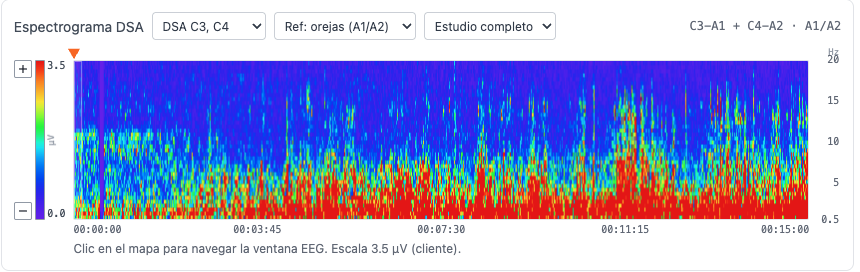
\includegraphics[width=\textwidth]{Chapter5/chapter5Figs/espectrograma_dsa.png}
    \caption{Visualización del espectrograma DSA
    implementado en EpilexIA.}
    \label{fig:espectrograma_dsa}
\end{figure}


\subsection[Pruebas automatizadas y limitaciones de la implementación]{Pruebas automatizadas y limitaciones de la \\implementación}

La implementación de los componentes de inteligencia artificial de
EpilexIA incorpora pruebas automatizadas orientadas a verificar
determinadas operaciones de los servicios de procesamiento y del motor
de clasificación. Estas pruebas permiten comprobar comportamientos
específicos del código, especialmente aquellos relacionados con la
validación de parámetros, el tratamiento de señales y la selección
de resultados. No obstante, su alcance debe distinguirse de una
validación integral del procesamiento electroencefalográfico y del
desempeño clínico del modelo.

Los proyectos \texttt{epilex-ia-api} y \texttt{epilex-ia-motor} cuentan con nueve archivos de pruebas automatizadas, que reúnen 64 casos.
Ambos utilizan el módulo \texttt{unittest} de Python y sus mecanismos de simulación de dependencias.
Las pruebas son unitarias y verifican el código de integración, no el desempeño del modelo.

El Cuadro~\ref{tab:pruebas_componentes_ia} resume las pruebas por grupo y el resultado de su ejecución.
Se ejecutaron los 64 casos y todos finalizaron satisfactoriamente.

\begin{table}[htbp]
    \centering
    \caption{Pruebas automatizadas de los componentes de inteligencia artificial y resultado de su ejecución.}
    \label{tab:pruebas_componentes_ia}
    \small
    \begin{tabular}{|
        >{\raggedright\arraybackslash}p{0.15\textwidth}|
        >{\raggedright\arraybackslash}p{0.19\textwidth}|
        >{\raggedright\arraybackslash}p{0.29\textwidth}|
        >{\centering\arraybackslash}p{0.07\textwidth}|
        >{\centering\arraybackslash}p{0.14\textwidth}|}
        \hline
        \textbf{Componente} &
        \textbf{Grupo de pruebas} &
        \textbf{Qué verifica} &
        \textbf{Casos} &
        \textbf{Aprobados} \\
        \hline
        API &
        Modelo activo y ejecución &
        Resolución del modelo configurado, validación de sus parámetros y registro del umbral en cada ejecución. &
        21 & 21 \\
        \hline
        API &
        Contrato de anomalías &
        Formato de los resultados que consume la plataforma web. &
        1 & 1 \\
        \hline
        API &
        Regla de ventanas consecutivas &
        Que una ventana aislada no se señale y que una secuencia de ventanas sí. &
        3 & 3 \\
        \hline
        API &
        Inclusión de resultados en informes &
        Ventanas confirmadas y anotaciones manuales asociadas a los informes. &
        8 & 8 \\
        \hline
        API &
        Espectrogramas &
        Identificación de canales, tratamiento de señales planas, cálculo por partes y reducción temporal. &
        22 & 22 \\
        \hline
        Motor &
        Canales constantes &
        Que una señal constante no interrumpa el procesamiento. &
        4 & 4 \\
        \hline
        Motor &
        Regla de ventanas consecutivas &
        La misma regla, en el motor. &
        3 & 3 \\
        \hline
        Motor &
        Selección de resultados &
        Que solo se registren las ventanas que cumplen el umbral. &
        2 & 2 \\
        \hline
        \textbf{Total} &
        &
        &
        \textbf{64} &
        \textbf{64} \\
        \hline
    \end{tabular}
\end{table}

No se cuenta con una configuración para medir la cobertura de código, por lo que no se informa un porcentaje de cobertura.

En cuanto al alcance de las verificaciones, las pruebas
existentes no recorren de manera integral el procesamiento
de un estudio EEG, desde la lectura del archivo EDF hasta
la carga del modelo, la clasificación de las ventanas
temporales y el almacenamiento de las detecciones en una
instancia real de PostgreSQL. Tampoco se cuenta con
pruebas automatizadas de concurrencia entre múltiples
instancias del motor, cancelación de trabajos, control de
tiempos máximos de ejecución o recuperación ante
interrupciones.

Respecto del procesamiento, el motor requiere que el archivo
EDF contenga los canales necesarios para construir las
derivaciones del montaje esperado por el modelo. Cuando
algunas derivaciones no pueden construirse, el procedimiento
las completa para mantener la estructura requerida, y la
ejecución se interrumpe si no es posible construir ninguna.
La compatibilidad entre el paquete del modelo y el
procedimiento de análisis se verifica al inicio de cada
ejecución.

El procesamiento de registros extensos presenta
igualmente consideraciones relacionadas con el consumo
de memoria. Si bien la lectura de determinadas señales
se organiza por bloques, los datos transformados pueden
acumularse y concatenarse para las etapas posteriores.
No se cuenta con pruebas de rendimiento que permitan
establecer límites de memoria o tiempos máximos de
procesamiento bajo diferentes tamaños de registros.

En el caso de los espectrogramas DSA, las pruebas
numéricas verifican operaciones específicas del cálculo,
pero no abarcan el recorrido completo de una solicitud
HTTP con lectura de un archivo EDF real. Asimismo,
su generación se realiza bajo demanda y los resultados
se mantienen únicamente en mecanismos temporales de
caché, sin persistencia permanente. Esta modalidad
requiere repetir el cálculo cuando los resultados
almacenados temporalmente dejan de estar disponibles.

En conjunto, las pruebas automatizadas identificadas
constituyen mecanismos de verificación para operaciones
concretas de los componentes de inteligencia artificial.
No obstante, las limitaciones observadas y la ausencia
de pruebas integrales evidencian la necesidad de ampliar
las verificaciones sobre la compatibilidad del modelo,
la preparación de señales, la concurrencia y el
comportamiento del sistema ante registros extensos.

Finalmente, debe señalarse que las pruebas de \textit{software}
descritas no constituyen una evaluación del desempeño
clínico del clasificador. La determinación de métricas
como sensibilidad, especificidad o precisión requiere
procedimientos de validación independientes, con
conjuntos de datos y criterios de evaluación apropiados.


\section{Despliegue e integración de los componentes}

El despliegue de EpilexIA comprende la configuración y puesta en
funcionamiento de los componentes que conforman el sistema, así
como el establecimiento de los mecanismos necesarios para su
comunicación y acceso a los recursos compartidos. La implementación
se organiza en proyectos independientes que incluyen la interfaz
web, el \textit{backend} clínico, la base de datos clínica, la API de
inteligencia artificial y el motor de procesamiento.

Para facilitar la construcción y ejecución de estos componentes,
se utilizan contenedores Docker y archivos de configuración
Docker Compose. Esta organización permite definir las dependencias
de ejecución, los puertos de comunicación, las variables de
entorno y los recursos de almacenamiento necesarios para cada
servicio.

La integración se realiza mediante una red Docker compartida,
servicios HTTP y mecanismos de persistencia. Asimismo, se
emplean volúmenes para conservar la información de las bases
de datos y permitir el acceso a los archivos electroencefalográficos
y a los modelos de clasificación.

En los siguientes apartados se describe la organización del
entorno de despliegue, la configuración de los contenedores,
las redes y los volúmenes, así como los mecanismos de
comunicación entre los componentes y las principales
consideraciones operativas de la implementación.

\subsection{Organización del entorno de despliegue}

La organización del entorno de despliegue de EpilexIA se basa
en la separación de sus componentes funcionales en cinco
proyectos. Cada uno dispone de sus propios archivos de
configuración y mecanismos de ejecución, lo que permite
administrar de manera diferenciada la interfaz web, los
servicios clínicos, la persistencia de datos y el procesamiento
de inteligencia artificial.

El proyecto de la interfaz web, denominado
\texttt{epilexIa-web-front-end}, utiliza React y TypeScript.
Durante el desarrollo, la aplicación se ejecuta mediante Vite,
mientras que su distribución contenedorizada comprende una
etapa de compilación y una etapa de publicación de los
archivos estáticos mediante Nginx. Este servidor también
actúa como intermediario para las solicitudes dirigidas
al \textit{backend} clínico.

El proyecto \texttt{epilexIa-back-end} implementa los
servicios clínicos mediante Java 21 y Spring Boot. La
aplicación se empaqueta como un archivo WAR y se despliega
sobre el servidor de aplicaciones WildFly 39. Su entorno
de ejecución incorpora las herramientas necesarias para
el procesamiento de videos y dispone de configuraciones
para conectarse con la base de datos clínica y con la
API de inteligencia artificial.

La persistencia de la información clínica se encuentra
organizada en el proyecto \texttt{epilexIa-database},
que utiliza PostgreSQL 17. Su configuración contempla
un contenedor de base de datos, almacenamiento persistente
y \textit{scripts} SQL destinados a la inicialización del esquema
en instalaciones nuevas.

Por su parte, el proyecto \texttt{epilex-ia-api} implementa
los servicios de inteligencia artificial mediante FastAPI,
ejecutado con Uvicorn. Este componente utiliza una instancia
independiente de PostgreSQL 16 para administrar las ejecuciones,
sus estados y los resultados del procesamiento. También
incorpora los mecanismos necesarios para gestionar las
migraciones del esquema mediante Alembic.

El proyecto \texttt{epilex-ia-motor} contiene el motor de
procesamiento de inteligencia artificial, implementado
en Python. A diferencia de los servicios web, este componente
se ejecuta como un proceso de trabajo independiente, sin
exponer una interfaz HTTP. Este proceso consulta la base de datos de inteligencia artificial para
recuperar los trabajos pendientes, ejecutar el análisis
de las señales EEG y almacenar los resultados obtenidos.

Cada proyecto dispone de una configuración Docker Compose
independiente. La comunicación entre los servicios se
establece mediante una red Docker externa compartida,
denominada \texttt{epilexia-net}, y mediante los mecanismos
de conexión definidos para cada componente. Esta
organización requiere que determinados recursos, como
la red y los volúmenes compartidos, estén disponibles
antes de iniciar los servicios que dependen de ellos.

Además de las configuraciones individuales, existe una configuración conjunta que reúne todos los servicios y que se utiliza en el despliegue en la nube descrito en la subsección siguiente.

\subsection{Entorno de despliegue en la nube}
\label{subsec:despliegue-nube}

EpilexIA se encuentra desplegado en infraestructura en la nube provista por la empresa BigQ, socio del sector privado del proyecto.
Sobre este entorno se realizaron las pruebas documentadas en el Anexo~\ref{pruebas_evaluacion} y las sesiones de validación con la especialista del IPS, quien accede al sistema por internet desde el hospital.

El despliegue reúne en un servidor los componentes descritos en la subsección anterior, ejecutados como contenedores mediante una configuración conjunta de Docker Compose.
Un servidor Nginx actúa como punto único de entrada: publica la aplicación web y encamina las solicitudes hacia el \textit{backend} clínico.
Las bases de datos, la API de inteligencia artificial y el motor de procesamiento no se exponen a internet y se comunican únicamente a través de una red interna.
Los archivos EEG y los modelos entrenados se almacenan en volúmenes compartidos entre los servicios que los requieren.

El acceso de los usuarios se realiza mediante HTTPS, bajo un dominio provisto por la empresa, cuya infraestructura incorpora además mecanismos de protección perimetral.
De este modo se atiende el requerimiento RNF-SEG-003.
La administración de estos elementos corresponde al proveedor de infraestructura y no forma parte del alcance de este trabajo.

Este entorno constituye la base operativa del sistema durante el proceso de transferencia al IPS, que prevé su despliegue en servidores propios de la institución.

\subsection{Contenedorización y configuración de servicios}

La contenedorización de los componentes de EpilexIA se implementa
mediante Docker, utilizando archivos \texttt{Dockerfile} para definir los
entornos de ejecución y configuraciones Docker Compose para
administrar los servicios asociados a cada proyecto. Esta
organización permite establecer las dependencias necesarias,
los comandos de inicio, las variables de entorno y los recursos
requeridos para el funcionamiento de las aplicaciones.

En el \textit{frontend}, la construcción de la imagen utiliza un
procedimiento de múltiples etapas. Inicialmente, se emplea
un entorno Node.js para instalar las dependencias y generar
los archivos estáticos de la aplicación mediante el proceso
de compilación de Vite. Posteriormente, los archivos
generados se incorporan a una imagen de Nginx, encargada
de publicar la interfaz web y atender las solicitudes
HTTP de los usuarios.

La configuración de Nginx también contempla el
encaminamiento de determinadas solicitudes hacia el
\textit{backend} clínico. De esta manera, el servidor web
permite distribuir los recursos estáticos del \textit{frontend}
y actuar como intermediario para las operaciones que
requieren acceder a los servicios REST del sistema.

Para el \textit{backend} clínico, la construcción y ejecución
se organizan alrededor de una aplicación Java empaquetada
en formato WAR. El artefacto generado se despliega
sobre una imagen de WildFly 39, que proporciona el
entorno de ejecución de los servicios desarrollados
con Spring Boot. La configuración del contenedor
incorpora las dependencias necesarias para las
operaciones de procesamiento y conversión de videos,
así como los parámetros de conexión con los servicios
externos utilizados por la aplicación.

La base de datos clínica se ejecuta mediante un
contenedor PostgreSQL 17. Su configuración Docker
Compose establece los parámetros de inicialización
de la instancia, la exposición del servicio y la
asociación con los recursos de almacenamiento
persistente. Asimismo, contempla la utilización
de \textit{scripts} SQL para preparar las estructuras
necesarias cuando se crea una instalación nueva.

En el caso de la API de inteligencia artificial,
la imagen de ejecución incorpora un entorno Python
con las dependencias requeridas por FastAPI,
SQLAlchemy y los procedimientos de procesamiento
implementados en este componente. El servicio
HTTP se inicia mediante Uvicorn y utiliza
parámetros de configuración para establecer
la conexión con su base de datos PostgreSQL
y gestionar la cola de trabajos de inteligencia artificial.

La configuración del proyecto de la API también
contempla una instancia PostgreSQL 16 destinada
a conservar la información de las ejecuciones
y los resultados del análisis. La administración
de los cambios del esquema se realiza mediante
Alembic, manteniendo diferenciada esta base de
datos de la utilizada por los servicios clínicos.

Por su parte, el motor de inteligencia artificial
dispone de un entorno contenedorizado basado en
Python, con las bibliotecas necesarias para
la lectura de registros EEG, la extracción de
características y la aplicación del modelo de
clasificación. El contenedor ejecuta un proceso de trabajo que
consulta las solicitudes disponibles en PostgreSQL
y desarrolla el procesamiento correspondiente,
sin necesidad de publicar un servicio HTTP propio.

Las configuraciones Docker Compose permiten
establecer los servicios, las variables de entorno,
las asociaciones de almacenamiento y las condiciones
necesarias para su ejecución. Sin embargo, al
encontrarse distribuidas entre proyectos independientes,
la puesta en funcionamiento del sistema requiere
considerar previamente la disponibilidad de los
recursos compartidos y de los servicios de los
que depende cada componente.

La utilización de contenedores facilita la
reproducción de los entornos de ejecución y
permite mantener diferenciadas las dependencias
del \textit{frontend}, el \textit{backend} clínico y los componentes
de inteligencia artificial. No obstante, esta
organización no elimina la necesidad de configurar
correctamente las conexiones, las rutas de archivos
y los recursos persistentes utilizados por el sistema.


El Cuadro~\ref{tab:componentes-contenedorizados} resume los
principales componentes de ejecución de EpilexIA, indicando
las tecnologías utilizadas y las responsabilidades que
cumplen dentro del entorno contenedorizado.

\begin{table}[htbp]
    \centering
    \caption{Componentes contenedorizados del sistema EpilexIA.}
    \label{tab:componentes-contenedorizados}
    \small
    \begin{tabularx}{\textwidth}{|
        >{\raggedright\arraybackslash}p{0.27\textwidth}|
        >{\raggedright\arraybackslash}p{0.27\textwidth}|
        >{\raggedright\arraybackslash}X|}
        \hline
        \textbf{Componente} &
        \textbf{Entorno de ejecución} &
        \textbf{Responsabilidad principal} \\
        \hline

        \textit{Frontend} &
        Node.js (compilación) y Nginx (ejecución) &
        Compilación y publicación de la interfaz web. \\
        \hline

        \textit{backend} clínico &
        Java 21 y WildFly 39 &
        Ejecución de los servicios clínicos y las operaciones de negocio. \\
        \hline

        Base de datos clínica &
        PostgreSQL 17 &
        Almacenamiento persistente de la información clínica. \\
        \hline

        API de inteligencia artificial &
        Python, FastAPI y Uvicorn &
        Recepción de solicitudes y administración de ejecuciones y resultados. \\
        \hline

        Base de datos de inteligencia artificial &
        PostgreSQL 16 &
        Persistencia de ejecuciones, cola de trabajos y resultados del análisis. \\
        \hline

        Motor de inteligencia artificial &
        Python &
        Procesamiento de señales EEG y ejecución del modelo de clasificación. \\
        \hline
    \end{tabularx}
\end{table}


\subsection{Configuración de redes, puertos y volúmenes}

La integración de los componentes contenedorizados de EpilexIA
requiere configurar los mecanismos de comunicación entre
servicios y los recursos de almacenamiento utilizados durante
su ejecución. Para ello, las configuraciones Docker Compose
contemplan redes, volúmenes y variables de entorno que permiten
establecer las conexiones necesarias y mantener disponibles
los datos y archivos utilizados por el sistema.

La comunicación entre los contenedores se organiza mediante
una red Docker externa compartida, denominada
\texttt{epilexia-net}. Esta red permite que los servicios
pertenecientes a distintos proyectos puedan comunicarse
utilizando los nombres y direcciones definidos en sus
respectivas configuraciones. Al tratarse de un recurso
externo, su disponibilidad debe garantizarse antes de
iniciar los contenedores que dependen de ella.

La utilización de una red compartida permite establecer
la comunicación interna entre el \textit{backend} clínico, los
servicios de persistencia y la API de inteligencia
artificial. De esta manera, las operaciones que requieren
acceder a otros componentes pueden realizarse mediante
las conexiones configuradas en el entorno de ejecución,
sin depender exclusivamente de los puertos publicados
hacia el equipo anfitrión.

Por otra parte, las configuraciones contemplan la
publicación de determinados puertos para permitir
el acceso a los servicios desde el exterior de los
contenedores. Estos mecanismos se utilizan para
atender las solicitudes HTTP dirigidas a la interfaz
web y a los servicios que requieren comunicación
externa. La asignación de puertos depende de la
configuración particular de cada proyecto y del
entorno donde se realiza el despliegue.


En relación con la persistencia, las instancias
PostgreSQL utilizadas por EpilexIA disponen de
recursos de almacenamiento asociados a sus
respectivos contenedores. Estos recursos permiten
conservar los archivos de datos de las bases clínica
y de inteligencia artificial cuando los contenedores
se detienen o se recrean, siempre que se mantengan
los volúmenes o directorios persistentes
correspondientes.


La separación entre ambas instancias de PostgreSQL
también se mantiene en el entorno contenedorizado.
La base de datos clínica conserva la información
administrada por el \textit{backend}, mientras que la base
de datos de inteligencia artificial almacena las
ejecuciones, los estados, la cola persistente de
trabajos y los resultados del procesamiento.
Cada componente utiliza los parámetros de conexión
correspondientes a su propia instancia.

Además de las bases de datos, el sistema requiere
acceso a los archivos asociados a los estudios EEG.
Estos archivos se conservan fuera de las tablas
relacionales y se ponen a disposición de los
componentes que necesitan utilizarlos mediante
rutas y recursos de almacenamiento configurados
en el entorno. Esta organización permite mantener
separados los archivos de señales de la información
estructurada almacenada en PostgreSQL.


En particular, el \textit{backend} clínico administra las operaciones relacionadas con la recepción y el almacenamiento de los archivos de los estudios, mientras que los componentes de inteligencia artificial requieren acceder a los archivos EEG para ejecutar los procedimientos de análisis. Por este motivo, las rutas utilizadas por los distintos servicios deben corresponder con las ubicaciones de almacenamiento disponibles en sus respectivos entornos de ejecución.


El motor de inteligencia artificial también
necesita acceder al archivo del modelo de
clasificación previamente entrenado. La ubicación
de este recurso se establece mediante los
parámetros de configuración del entorno,
permitiendo que el proceso de inferencia
localice el archivo serializado sin incorporarlo
a la información almacenada en las bases de datos.

La configuración de las conexiones y rutas
se apoya en variables de entorno y parámetros
definidos para cada servicio. Entre ellos se
encuentran las direcciones de los componentes,
las credenciales de acceso a las bases de datos
y las ubicaciones de los recursos necesarios
para el procesamiento. Esta organización permite
diferenciar los parámetros propios del despliegue
de la lógica implementada en las aplicaciones.

No obstante, la distribución del sistema entre
varios proyectos implica que la correspondencia
entre nombres de servicios, redes, puertos y
rutas de almacenamiento debe mantenerse de
manera consistente. Una configuración incorrecta
de estos recursos puede impedir la comunicación
entre componentes o el acceso a los archivos
requeridos para ejecutar determinadas operaciones.

En conjunto, los mecanismos de red y almacenamiento
permiten integrar los servicios clínicos y de
inteligencia artificial, manteniendo diferenciadas
sus responsabilidades y recursos de persistencia.
Su correcta configuración constituye una condición
necesaria para el funcionamiento coordinado del
sistema en un entorno contenedorizado.


\subsection{Integración y comunicación entre componentes}

La integración de los componentes de EpilexIA se implementa
mediante mecanismos de comunicación que permiten coordinar
las operaciones de la interfaz web, el \textit{backend} clínico y los
servicios de inteligencia artificial. Esta organización
mantiene diferenciadas las responsabilidades de cada
componente, estableciendo los intercambios de información
necesarios para atender las funcionalidades del sistema.

La interfaz web constituye el punto de interacción con
los usuarios. Desde ella se realizan las solicitudes
relacionadas con la gestión de estudios EEG, la consulta
de información clínica, la visualización de señales y
el acceso a los resultados del procesamiento automatizado.
Estas operaciones se comunican con el \textit{backend} clínico
mediante solicitudes HTTP, utilizando principalmente
estructuras JSON para el intercambio de información.

En el entorno contenedorizado, Nginx publica los recursos
estáticos de la interfaz web y actúa como intermediario
para determinadas solicitudes dirigidas al \textit{backend}.
Esta configuración permite que el \textit{frontend} acceda a los
servicios REST sin establecer directamente las conexiones
internas utilizadas por los demás componentes del sistema.

El \textit{backend} clínico, implementado con Spring Boot, concentra
las operaciones relacionadas con la información de los
pacientes, los estudios electroencefalográficos, los
informes médicos y las funcionalidades administrativas.
Para conservar y recuperar estos datos, utiliza los
mecanismos de persistencia asociados a la base de datos
clínica PostgreSQL 17.

Las operaciones que requieren procesamiento de inteligencia
artificial se coordinan mediante la comunicación entre el
\textit{backend} clínico y la API desarrollada con FastAPI. El
\textit{backend} envía las solicitudes de análisis y posteriormente
consulta la información disponible sobre las ejecuciones,
sus estados y los resultados obtenidos. Este intercambio
se realiza mediante servicios HTTP, sin que el \textit{backend}
clínico tenga que ejecutar directamente los procedimientos
de extracción de características o clasificación de
señales EEG.

La API de inteligencia artificial utiliza su propia
base de datos PostgreSQL 16 para administrar las
ejecuciones y conservar los resultados del procesamiento.
Las solicitudes registradas por la API quedan disponibles para el motor
independiente de inteligencia artificial, que recupera
los trabajos pendientes y ejecuta las operaciones
correspondientes.

La coordinación entre la API y el motor se realiza
mediante los registros compartidos en la base de datos
de inteligencia artificial. Por tanto, no se requiere una comunicación HTTP directa entre ambos
componentes. El motor consulta los trabajos disponibles,
actualiza la información de las ejecuciones y registra
los resultados, mientras que la API proporciona los
servicios necesarios para su posterior recuperación.

La ejecución de los análisis también requiere el acceso
a los archivos EEG almacenados por el sistema. El \textit{backend}
clínico administra las operaciones de recepción y
almacenamiento de estos archivos, mientras que los
componentes de inteligencia artificial utilizan las
rutas configuradas para localizar los registros que
deben procesarse. De esta manera, la información
estructurada y los archivos de señales se mantienen
en recursos diferenciados, pero accesibles para las
operaciones que los requieren.


La arquitectura contempla la recuperación de los resultados persistidos mediante la API de inteligencia artificial, una vez finalizado el procesamiento. El \textit{backend} clínico utiliza estos servicios para poner la información disponible a disposición de la interfaz web, donde las detecciones pueden relacionarse con los intervalos temporales del estudio EEG. Este mecanismo permite consultar resultados previamente almacenados sin repetir las operaciones de procesamiento e inferencia. La verificación de esta consulta y de la ejecución completa del análisis se documenta en el Anexo~\ref{pruebas_evaluacion}.


Por otra parte, la generación de espectrogramas DSA
utiliza un mecanismo de integración diferente al de
las ejecuciones de clasificación. En este caso, el
\textit{backend} clínico solicita el procesamiento espectral
a la API de inteligencia artificial, que calcula
la representación requerida y devuelve los datos
necesarios para su visualización. Esta operación
se realiza bajo demanda, sin utilizar la cola
persistente de trabajos del motor independiente.

La integración también contempla mecanismos de
autenticación diferenciados. El acceso de los usuarios
a las funcionalidades clínicas se controla mediante
los mecanismos de seguridad del \textit{backend}, mientras
que la comunicación con los servicios protegidos
de la API de inteligencia artificial utiliza las
credenciales HTTP Basic configuradas para dicho
componente. Esta separación permite aplicar los
controles de acceso correspondientes a cada interfaz
de comunicación.

En conjunto, la integración implementada permite
coordinar las operaciones clínicas, el acceso a los
archivos EEG y los procedimientos de inteligencia
artificial mediante interfaces y recursos definidos.
La separación entre los componentes facilita mantener
diferenciadas sus responsabilidades, mientras que
los mecanismos de comunicación y persistencia
proporcionan los medios necesarios para el
funcionamiento conjunto de EpilexIA.


\subsection[Consideraciones operativas y limitaciones del despliegue]{Consideraciones operativas y limitaciones del \\despliegue}

La puesta en funcionamiento de EpilexIA requiere considerar
determinadas condiciones operativas derivadas de la
distribución del sistema en varios componentes independientes.
Aunque la utilización de contenedores Docker permite definir
los entornos de ejecución y sus dependencias, el funcionamiento
conjunto de las aplicaciones depende de la disponibilidad
de los servicios, las conexiones y los recursos compartidos
configurados para cada proyecto.

Una de las principales consideraciones corresponde a la
preparación del entorno antes de iniciar los contenedores.
Debido a que los proyectos utilizan configuraciones Docker
Compose independientes, determinados recursos deben existir
previamente para que los servicios puedan establecer sus
conexiones. Entre ellos se encuentra la red externa compartida
\texttt{epilexia-net}, utilizada para la comunicación entre
los componentes del sistema.

La inicialización de las bases de datos constituye otra
condición relevante. El \textit{backend} clínico requiere disponer
de la instancia PostgreSQL 17 y de las estructuras necesarias
para administrar la información del sistema. Por su parte,
la API de inteligencia artificial y el motor de procesamiento
dependen de la instancia PostgreSQL 16, utilizada para
conservar las ejecuciones, los resultados y la cola
persistente de trabajos.

La disponibilidad de estas instancias no depende únicamente
del inicio de sus respectivos contenedores. También es
necesario que los servicios de base de datos se encuentren
preparados para aceptar conexiones y que sus esquemas
dispongan de las estructuras requeridas por las aplicaciones.
En este sentido, los \textit{scripts} de inicialización de la base
de datos clínica y los mecanismos de migración utilizados
por la API de inteligencia artificial forman parte de las
consideraciones necesarias para preparar el entorno.

El acceso a los recursos de almacenamiento también requiere
una configuración consistente entre los componentes. Los
archivos EEG utilizados durante el procesamiento deben
encontrarse en ubicaciones accesibles para los servicios
que los necesitan. Asimismo, el motor de inteligencia
artificial debe disponer del archivo correspondiente al
modelo de clasificación previamente entrenado.

Estas condiciones implican que las rutas configuradas
dentro de los contenedores deben corresponder con los
recursos disponibles en el entorno de ejecución. Una configuración incorrecta de los directorios o de los volúmenes puede impedir la lectura de los archivos EEG, la localización del modelo o la conservación de la información persistente.


Otro aspecto operativo corresponde a la administración
de las variables de entorno. Las configuraciones de los
distintos proyectos incluyen parámetros relacionados con
las conexiones a las bases de datos, las direcciones de
los servicios, las credenciales de acceso y las rutas
de almacenamiento. La correspondencia entre estos valores
resulta necesaria para que los componentes puedan
intercambiar información y utilizar los recursos previstos.

En particular, la comunicación entre el \textit{backend} clínico
y la API de inteligencia artificial depende de que las
direcciones y credenciales configuradas sean compatibles
con los servicios disponibles. De manera similar, la API y el motor de inteligencia artificial
deben compartir la configuración de acceso a la base de datos
de inteligencia artificial.

La organización mediante proyectos independientes también
introduce consideraciones relacionadas con el orden de
puesta en funcionamiento. Los componentes que dependen
de servicios de persistencia, redes compartidas o recursos
de almacenamiento requieren que dichos elementos estén
disponibles antes de realizar las operaciones que los
utilizan. Por consiguiente, el inicio de los contenedores
no garantiza por sí solo que todas las funcionalidades
del sistema se encuentren inmediatamente disponibles.

En cuanto a las limitaciones del despliegue, el despliegue se encuentra distribuido entre
configuraciones Docker Compose individuales y una configuración conjunta utilizada en la nube.
No se dispone de un procedimiento único y completamente automatizado que abarque la preparación de todos los recursos, la inicialización de los servicios y la verificación integral de su funcionamiento.

Esta organización requiere coordinar las configuraciones
de los distintos proyectos y comprobar la disponibilidad
de sus dependencias. Asimismo, los cambios realizados
en nombres de servicios, variables de entorno, rutas
de almacenamiento o parámetros de conexión pueden
requerir ajustes en más de un componente para conservar
la integración del sistema.

Por otra parte, la utilización de una cola persistente
permite desacoplar la recepción de solicitudes de
inteligencia artificial de la ejecución de los trabajos.
Sin embargo, la disponibilidad del procesamiento
automatizado depende de que el motor se encuentre en
funcionamiento y pueda acceder tanto a la base de datos
de inteligencia artificial como a los archivos necesarios
para realizar el análisis.

La implementación dispone de mecanismos para registrar
los estados de las ejecuciones e identificar determinadas
situaciones de error. No obstante, estos mecanismos no
equivalen por sí mismos a una solución completa de
supervisión operativa, recuperación automática ante
cualquier interrupción o garantía de disponibilidad
continua de los servicios.

Finalmente, no se evaluaron la escalabilidad, la tolerancia
a fallos ni el comportamiento del sistema bajo cargas elevadas.
La evaluación de estas propiedades requiere pruebas
específicas y condiciones de ejecución definidas,
que deben distinguirse de la descripción de los
mecanismos de contenedorización implementados.

En conjunto, las consideraciones identificadas muestran
que el funcionamiento integrado de EpilexIA depende
tanto de la correcta configuración de sus componentes
como de la disponibilidad de las redes, los servicios
de persistencia y los recursos de almacenamiento.
La arquitectura contenedorizada proporciona una
organización diferenciada de los entornos de ejecución,
mientras que la coordinación de sus dependencias
constituye un aspecto fundamental para la puesta
en funcionamiento del sistema.

La Figura~\ref{fig:arquitectura-despliegue}
presenta una representación general de la integración
de los componentes de EpilexIA en el entorno
contenedorizado. Se distinguen las comunicaciones
HTTP entre la interfaz web, el \textit{backend} clínico y
la API de inteligencia artificial, así como las
conexiones con las bases de datos y los recursos
de almacenamiento necesarios para el procesamiento
de los estudios EEG. Asimismo, se representa
la interacción del motor de inteligencia artificial
con la base de datos que administra la cola
persistente de trabajos.

% En el preámbulo, si todavía no están cargados:
% \usepackage{tikz}
% \usetikzlibrary{arrows.meta,positioning,fit,calc}

\begin{figure}[p]
\centering
\begin{adjustbox}{max width=0.95\textwidth}
\begin{tikzpicture}[
    font=\small,
    >=Latex,
    componente/.style={
        draw,
        rounded corners=3pt,
        align=center,
        minimum width=4.4cm,
        minimum height=1.1cm,
        fill=blue!6
    },
    bd/.style={
        draw,
        rounded corners=3pt,
        align=center,
        minimum width=3.4cm,
        minimum height=1cm,
        fill=green!8
    },
    recurso/.style={
        draw,
        rounded corners=3pt,
        align=center,
        minimum width=3.4cm,
        minimum height=0.9cm,
        fill=orange!9
    },
    conexion/.style={-Latex, thick},
    bidireccional/.style={Latex-Latex, thick}
]

\node[componente] (frontend)
    {Interfaz web\\
     \footnotesize React, TypeScript y Nginx};

\node[componente, below=1.25cm of frontend] (backend)
    {\textit{Backend} clínico\\
     \footnotesize Spring Boot y WildFly 39};

\node[componente, below=1.45cm of backend] (api)
    {API de inteligencia artificial\\
     \footnotesize FastAPI y Uvicorn};

\node[componente, below=2.0cm of api] (motor)
    {Motor de inteligencia artificial\\
     \footnotesize Python};

\node[bd, left=1.3cm of backend] (bdclinica)
    {Base de datos clínica\\
     \footnotesize PostgreSQL 17};

\node[bd, right=1.3cm of api] (bdia)
    {Base de datos de IA\\
     \footnotesize PostgreSQL 16};

\node[recurso, left=1.3cm of motor] (archivos)
    {Archivos EEG\\
     \footnotesize Almacenamiento compartido};

\node[recurso, right=1.3cm of motor] (modelo)
    {Modelo de clasificación\\
     \footnotesize Archivo serializado};

\draw[bidireccional] (frontend) --
    node[right, font=\scriptsize]{HTTP/REST} (backend);

\draw[bidireccional] (backend) --
    node[right, font=\scriptsize]{HTTP/REST} (api);

\draw[bidireccional] (backend) -- (bdclinica);

\draw[bidireccional] (api) -- (bdia);

\draw[bidireccional]
    (motor.north) -- ++(0,0.55)
    -| (bdia.south);

\draw[conexion] (archivos) -- (motor);

% El motor carga el modelo de clasificación serializado
\draw[conexion] (modelo.west) -- (motor.east);

\draw[conexion, dashed] (backend.south west) -|
    (archivos.north);

\node[
    draw,
    dashed,
    rounded corners=5pt,
    inner sep=12pt,
    fit=(frontend)(backend)(api)(motor)
        (bdclinica)(bdia)(archivos)(modelo),
    label={[font=\small]above:
        Red Docker compartida: \texttt{epilexia-net}}
] {};

\end{tikzpicture}
\end{adjustbox}
\caption{Arquitectura de despliegue e integración
de los componentes del sistema EpilexIA.}
\label{fig:arquitectura-despliegue}
\end{figure}

\clearpage
\lhead{\emph{Anexo C. Pruebas y evaluación}}

\chapter{Pruebas y evaluación}
\label{pruebas_evaluacion}

\section{Estrategia de pruebas}
\label{sec:estrategia_pruebas}

La estrategia de pruebas y evaluación de EpilexIA se orienta a verificar el comportamiento funcional del sistema, la integración entre sus componentes, el procesamiento y la visualización de señales electroencefalográficas, así como su rendimiento y usabilidad en el contexto de aplicación previsto. Para ello, se consideran procedimientos de verificación técnica y actividades de evaluación con usuarios, con el propósito de obtener evidencias sobre el cumplimiento de los requerimientos establecidos.

Se adopta principalmente un enfoque de pruebas de caja negra, mediante el cual se evalúa el comportamiento observable del sistema a partir de las entradas proporcionadas y las salidas obtenidas, sin requerir el conocimiento de los detalles internos de implementación. Este enfoque permite analizar EpilexIA desde la perspectiva de sus usuarios y de los servicios que ofrece, considerando operaciones como la gestión de pacientes y estudios, la carga de archivos EEG, la visualización de señales, el registro de anomalías, la ejecución del análisis mediante inteligencia artificial y la elaboración de informes médicos.

La estrategia contempla los siguientes ámbitos de evaluación:

\begin{itemize}
    \item \textbf{Pruebas funcionales:} orientadas a comprobar que las funcionalidades del sistema respondan a los requerimientos definidos y produzcan los resultados esperados ante diferentes condiciones de utilización.

    
    \item \textbf{Pruebas de integración:} destinadas a verificar la comunicación y el intercambio de información entre el \textit{frontend}, el \textit{backend}, las bases de datos y los componentes de inteligencia artificial.


    \item \textbf{Pruebas de procesamiento y visualización EEG:} enfocadas en evaluar la carga y representación de señales, la configuración de montajes, filtros y sensibilidad, la navegación temporal y el registro de anomalías. Sus resultados se presentan en los casos PF-05 a PF-09 y en la prueba de integración PI-05.

    \item \textbf{Pruebas de integración con inteligencia artificial:} dirigidas a comprobar la solicitud de análisis, el seguimiento de las ejecuciones y la recuperación y presentación de los resultados generados.

    \item \textbf{Pruebas de rendimiento:} previstas en la estrategia y no ejecutadas en el presente trabajo, destinadas a medir indicadores cuantitativos, como los tiempos de respuesta, la duración de las operaciones, el consumo de recursos computacionales y el comportamiento del sistema bajo diferentes condiciones de carga.

    \item \textbf{Evaluación de usabilidad:} realizada de forma exploratoria y cualitativa, orientada a analizar la eficacia, eficiencia y satisfacción de los usuarios al realizar tareas representativas de su actividad, considerando como referencia los principios establecidos en la norma ISO~9241-11.
\end{itemize}


Para las pruebas funcionales y de integración se utilizaron casos de prueba que especifican la funcionalidad evaluada, el procedimiento de ejecución y el resultado esperado. Las condiciones de cada ejecución y el resultado obtenido se documentan en la sección correspondiente a cada prueba. Esta estructura permitió documentar los comportamientos observados e identificar posibles diferencias respecto de los requerimientos del sistema.


En cuanto al rendimiento, se contemplaron escenarios de medición reproducibles, considerando las características del entorno de ejecución, el tamaño de los archivos procesados y las condiciones de carga. Estas evaluaciones quedaron pendientes de ejecución sistemática, por lo que no se presentan resultados cuantitativos sobre tiempos de respuesta, consumo de recursos o comportamiento bajo carga.


La evaluación de usabilidad se consideró a partir de tareas representativas del flujo de trabajo clínico y del registro de observaciones realizadas durante la interacción con la plataforma. Si bien se contempló la posibilidad de utilizar instrumentos estandarizados, como el cuestionario System Usability Scale (SUS), la evaluación efectivamente realizada tuvo carácter exploratorio y no incluyó su aplicación. Por consiguiente, los resultados obtenidos se interpretan como observaciones cualitativas y no como una medición cuantitativa de la usabilidad.


Las pruebas de integración con el servicio de inteligencia artificial y las sesiones con la especialista se ejecutaron sobre la instancia del sistema desplegada en la nube, descrita en la Sección~\ref{subsec:despliegue-nube}.

La evaluación contó con la participación de una médica especialista en epileptología del Hospital Central del Instituto de Previsión Social (IPS), quien accedió a la instancia de EpilexIA desplegada en la infraestructura en la nube de BigQ (Sección~\ref{subsec:despliegue-nube}) desde las instalaciones hospitalarias, utilizando una cuenta individual con el perfil Especialista. Durante su utilización, la profesional comunicó verbalmente observaciones y sugerencias que fueron registradas por el equipo de desarrollo. Estas observaciones dieron lugar a un conjunto de mejoras funcionales, principalmente relacionadas con el visualizador EEG y las herramientas de análisis, que se detallan en el Cuadro~\ref{tab:observaciones-especialista}. Esta actividad se considera una evaluación exploratoria, dado que no incluyó la aplicación de cuestionarios estandarizados ni la medición sistemática de indicadores de usabilidad.


La estrategia de evaluación distingue entre las pruebas automatizadas existentes, las verificaciones funcionales realizadas durante el desarrollo y las evaluaciones adicionales previstas. Los resultados se documentaron según las evidencias disponibles, evitando considerar como ejecutadas aquellas pruebas para las cuales no se obtuvieron registros verificables.


Finalmente, las evidencias obtenidas servirán de base para analizar el cumplimiento de los requerimientos funcionales y no funcionales, así como para valorar los resultados del sistema en relación con los objetivos y la hipótesis planteados en la investigación.


\section{Pruebas funcionales}
\label{sec:pruebas_funcionales}

Las pruebas funcionales de EpilexIA tienen como finalidad verificar que las operaciones disponibles en el sistema respondan a los requerimientos establecidos y produzcan los resultados esperados ante diferentes condiciones de utilización. Para ello, se adopta un enfoque de caja negra, centrado en la interacción del usuario con la plataforma y en la observación de sus respuestas, sin considerar los detalles internos de implementación.

La evaluación contempla las principales funcionalidades asociadas al flujo de trabajo clínico, desde la autenticación y la gestión de pacientes hasta la visualización de estudios electroencefalográficos, el registro de anomalías y la elaboración de informes médicos. Asimismo, se consideran las restricciones de acceso correspondientes a los perfiles de usuario definidos en el sistema.

Los casos de prueba se estructuran mediante un identificador, la funcionalidad evaluada, el procedimiento de ejecución y el resultado esperado. Esta organización permite establecer criterios de verificación reproducibles y facilita el registro posterior de los resultados obtenidos.

El Cuadro~\ref{tab:casos_pruebas_funcionales} presenta los casos de prueba propuestos para la evaluación funcional de EpilexIA.


\begingroup
\small
\setlength{\tabcolsep}{4pt}
\renewcommand{\arraystretch}{1.2}


\begin{longtable}{|
>{\raggedright\arraybackslash}p{\dimexpr0.10\textwidth-2\tabcolsep-1.25\arrayrulewidth\relax}|
>{\raggedright\arraybackslash}p{\dimexpr0.22\textwidth-2\tabcolsep-1.25\arrayrulewidth\relax}|
>{\raggedright\arraybackslash}p{\dimexpr0.30\textwidth-2\tabcolsep-1.25\arrayrulewidth\relax}|
>{\raggedright\arraybackslash}p{\dimexpr0.38\textwidth-2\tabcolsep-1.25\arrayrulewidth\relax}|}


\caption{Casos de prueba funcionales definidos para EpilexIA.}
\label{tab:casos_pruebas_funcionales}\\
\hline

\textbf{ID} &
\textbf{Funcionalidad} &
\textbf{Procedimiento} &
\textbf{Resultado esperado} \\
\hline
\endfirsthead

\multicolumn{4}{c}{\textit{Continuación del Cuadro \thetable}}\\
\hline
\textbf{ID} &
\textbf{Funcionalidad} &
\textbf{Procedimiento} &
\textbf{Resultado esperado} \\
\hline
\endhead

\hline
\endfoot


PF-01 &
Autenticación de usuarios &
Ingresar al sistema con credenciales válidas. &
El sistema permite el acceso y presenta las opciones correspondientes al perfil del usuario. \\
\hline

PF-02 &
Validación de credenciales &
Intentar iniciar sesión con credenciales incorrectas. &
El sistema rechaza el acceso y presenta un mensaje de error. \\
\hline

PF-03 &
Registro de pacientes &
Registrar un nuevo paciente desde el formulario de creación de estudios EEG. &
El sistema almacena la información del paciente y permite seleccionarlo para asociarlo a un estudio EEG. \\
\hline

PF-04 &
Registro de estudios EEG &
Crear un estudio asociado a un paciente existente. &
El estudio queda registrado y vinculado al paciente correspondiente. \\
\hline

PF-05 &
Carga de archivos EEG &
Cargar un archivo EEG en un formato admitido. &
El sistema acepta el archivo y permite consultar el estado de la carga. \\
\hline

PF-06 &
Visualización de señales EEG &
Abrir un estudio que contenga señales EEG disponibles. &
El visualizador representa las señales y sus canales correspondientes. \\
\hline

PF-07 &
Configuración de montajes &
Seleccionar un montaje EEG disponible. &
Las señales se presentan según la configuración del montaje seleccionado. \\
\hline

PF-08 &
Configuración de filtros &
Modificar los parámetros de filtrado de las señales EEG. &
El sistema aplica los parámetros admitidos y actualiza la representación de las señales. \\
\hline

PF-09 &
Registro manual de anomalías &
Seleccionar un intervalo temporal y registrar una anomalía. &
La anomalía queda asociada al estudio y al intervalo seleccionado. \\
\hline

PF-10 &
Consulta de resultados de IA &
Consultar los resultados de un estudio con análisis de IA finalizado. &
El sistema presenta los resultados disponibles y sus referencias temporales. \\
\hline

PF-11 &
Elaboración de informes médicos &
Crear y guardar un informe asociado a un estudio. &
El informe queda almacenado y puede consultarse posteriormente. \\
\hline

PF-12 &
Restricción de edición de informes &
Intentar modificar un informe perteneciente a otro especialista. &
El sistema impide la modificación por parte de un usuario no autorizado. \\
\hline

PF-13 &
Cierre de informes médicos &
Cerrar un informe médico en estado Borrador. &
El informe cambia al estado Cerrado y no admite modificaciones posteriores. \\
\hline

PF-14 &
Control de acceso por roles &
Intentar acceder a una operación sin los permisos necesarios. &
El sistema restringe la operación y evita su ejecución. \\
\hline

PF-15 &
Consulta de auditoría &
Consultar los registros de auditoría con un usuario autorizado. &
El sistema presenta los registros disponibles según los permisos del usuario. \\
\hline

\end{longtable}
\endgroup

Los casos presentados constituyen una base para la verificación funcional de la plataforma. Su ejecución requiere disponer de usuarios de prueba con diferentes perfiles, pacientes y estudios de referencia, archivos EEG compatibles y datos que permitan comprobar tanto las operaciones autorizadas como las restricciones previstas.


Para cada caso se registró el resultado observado y se estableció su estado como aprobado, no aprobado o no ejecutado, según las evidencias disponibles. La aprobación se determinó mediante la correspondencia entre el comportamiento observado y el resultado esperado, mientras que los casos no ejecutados quedaron identificados como tales.


A partir de las observaciones realizadas por la médica especialista en epileptología durante la evaluación exploratoria en el Hospital Central del IPS, se incorporaron mejoras a la plataforma (Cuadro~\ref{tab:observaciones-especialista}). La definición de casos de prueba adicionales que verifiquen dichas mejoras de manera sistemática queda prevista como actividad posterior.


Los resultados obtenidos permitieron identificar posibles desviaciones funcionales y aportar evidencias al análisis del cumplimiento de los requerimientos del sistema.


\subsection{Resultados de las pruebas de autenticación}
\label{subsec:resultados_autenticacion}

Las pruebas iniciales de autenticación comprendieron dos casos orientados a verificar el acceso mediante credenciales válidas y el rechazo de credenciales incorrectas.

En el caso PF-01, se utilizó una cuenta con perfil Especialista. El sistema permitió el inicio de sesión y presentó el panel de control correspondiente, con los indicadores generales y las opciones de navegación disponibles para el usuario autenticado. El resultado obtenido coincidió con el comportamiento esperado, por lo que el caso se clasificó como aprobado.

En la Figura~\ref{fig:pf01_dashboard} se presenta el panel de control visualizado después de la autenticación satisfactoria.

\begin{figure}[!htbp]
    \centering
    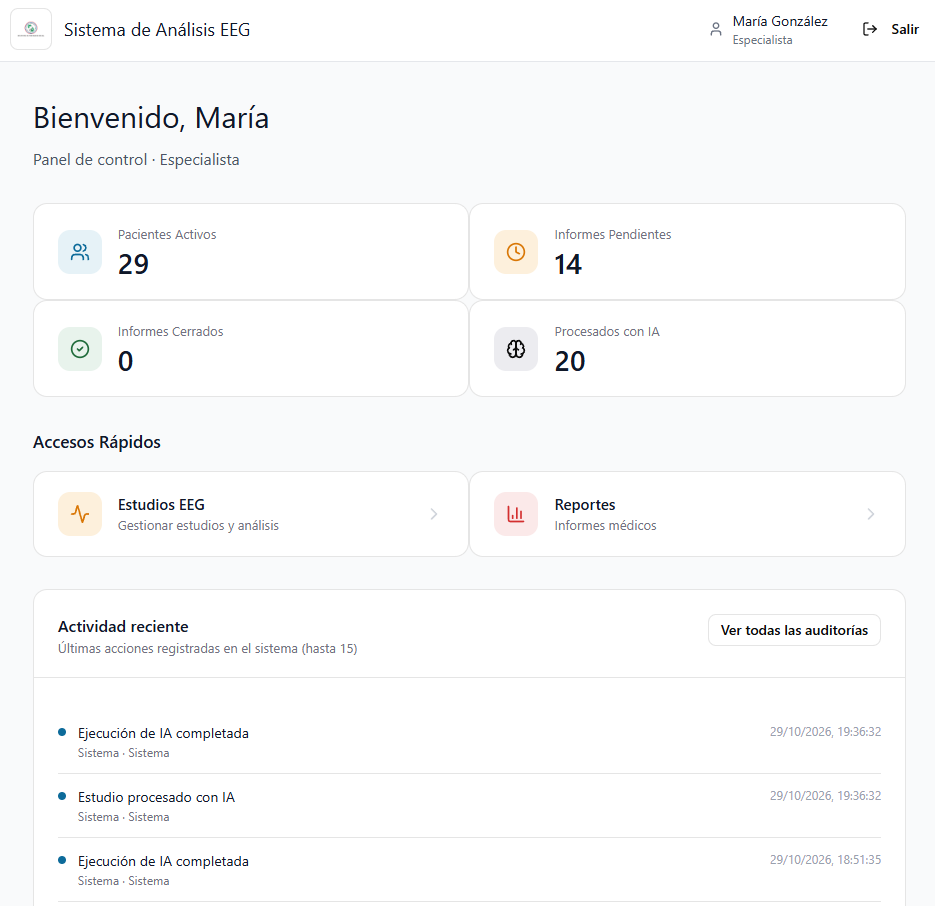
\includegraphics[width=0.95\textwidth]{Chapter6/Chapter6Figs/pf01_dashboard_especialista.png}
    \caption{Panel de control de EpilexIA después del inicio de sesión con perfil Especialista.}
    \label{fig:pf01_dashboard}
\end{figure}

En el caso PF-02, se intentó iniciar sesión utilizando una contraseña incorrecta. Como respuesta, la plataforma mostró el mensaje ``Credenciales inválidas'' e impidió el acceso al sistema.

Adicionalmente, después de cerrar una sesión válida, se intentó acceder directamente a la dirección del panel de control mediante un enlace previamente guardado. El sistema presentó nuevamente el formulario de autenticación, sin permitir la visualización del contenido protegido.

La Figura~\ref{fig:pf02_validacion} presenta las evidencias correspondientes al rechazo de credenciales incorrectas y a la restricción de acceso al panel de control.

\begin{figure}[!htbp]
    \centering

    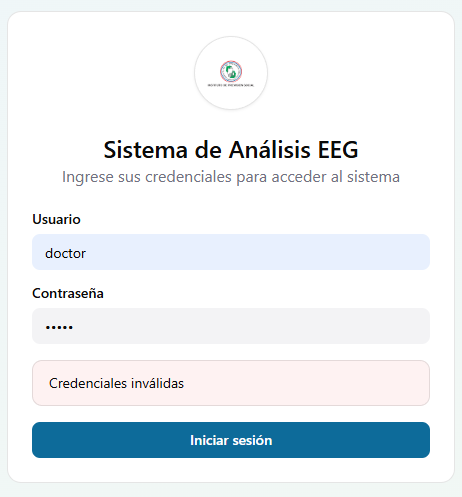
\includegraphics[width=0.52\textwidth]{Chapter6/Chapter6Figs/pf02_credenciales_invalidas.png}

    \par\smallskip
    {\small (a) Mensaje de error ante credenciales incorrectas.}

    \medskip

    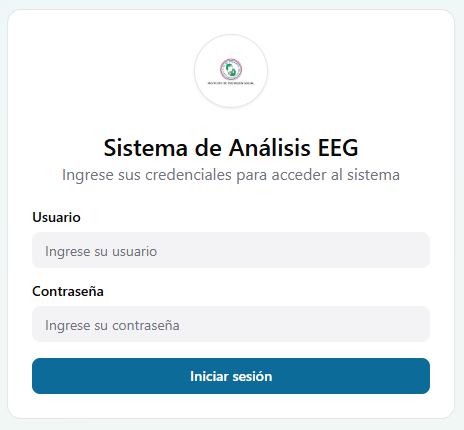
\includegraphics[width=0.52\textwidth]{Chapter6/Chapter6Figs/pf02_acceso_restringido.png}

    \par\smallskip
    {\small (b) Formulario de autenticación al intentar acceder al panel de control sin una sesión válida.}

    \caption{Validación de credenciales y restricción de acceso en EpilexIA.}
    \label{fig:pf02_validacion}
\end{figure}

Los comportamientos observados en los casos PF-01 y PF-02 coincidieron con los resultados esperados. En consecuencia, ambos casos fueron clasificados como aprobados dentro de las condiciones evaluadas. La verificación de acceso directo se limitó a la ruta del panel de control y no constituye una evaluación exhaustiva de la seguridad del sistema.


\subsection{Resultados de la prueba de registro de pacientes}

La prueba funcional PF-03 tuvo como objetivo verificar el registro de un nuevo paciente y su posterior disponibilidad para la asociación con un estudio electroencefalográfico. Esta funcionalidad se encuentra integrada en el proceso de creación de estudios EEG, desde el cual el usuario puede seleccionar un paciente existente o registrar uno nuevo.

Para ejecutar la prueba, se accedió al formulario de creación de estudios EEG y se seleccionó la opción de registro de un nuevo paciente. Se completaron los campos correspondientes a la identificación, los datos personales y la información de contacto, utilizando datos ficticios destinados exclusivamente a la evaluación funcional.

Una vez completado el formulario, se ejecutó la operación de registro. Posteriormente, se utilizó el campo de búsqueda de pacientes del formulario de creación de estudios EEG para comprobar la disponibilidad del registro generado.

El sistema permitió localizar al paciente mediante sus datos de identificación y lo presentó entre las opciones disponibles para su selección. Este comportamiento permitió verificar que la información registrada podía recuperarse desde la interfaz y utilizarse en el proceso de asociación de pacientes con estudios EEG.

La Figura~\ref{fig:pf03_registro_paciente} presenta las evidencias correspondientes al formulario completado y a la consulta posterior del paciente registrado.

El resultado observado coincidió con el comportamiento esperado para el caso PF-03, por lo que la prueba se clasificó como aprobada. La evaluación se limitó al registro y la consulta del paciente, sin incluir la creación de un estudio EEG asociado, procedimiento contemplado en el caso PF-04.


\begin{figure}[!htbp]
    \centering

    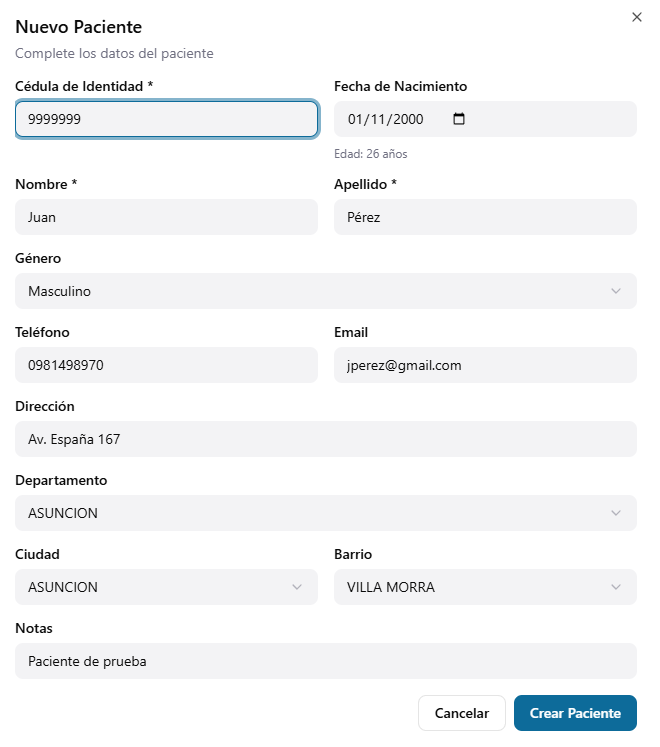
\includegraphics[
        width=0.85\textwidth,
        height=0.53\textheight,
        keepaspectratio
    ]{Chapter6/Chapter6Figs/pf03_formulario_paciente.png}

    \par\smallskip
    {\small (a) Formulario de registro completado con datos ficticios.}

    \medskip

    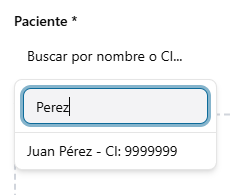
\includegraphics[
        width=0.85\textwidth,
        height=0.22\textheight,
        keepaspectratio
    ]{Chapter6/Chapter6Figs/pf03_paciente_registrado.png}

    \par\smallskip
    {\small (b) Paciente registrado y disponible en el selector de pacientes.}

    \caption{Registro y consulta de un paciente en EpilexIA.}
    \label{fig:pf03_registro_paciente}
\end{figure}

\FloatBarrier

\subsection{Resultados de las pruebas de registro de estudios y carga de archivos EEG}

Las pruebas funcionales PF-04 y PF-05 se ejecutaron de manera conjunta, dado que en EpilexIA el archivo EEG se carga en la misma operación en la que se registra el estudio.
La prueba PF-04 tuvo como objetivo verificar la creación de un estudio electroencefalográfico y su correcta asociación con un paciente previamente registrado.
La prueba PF-05 tuvo como objetivo verificar la aceptación de archivos electroencefalográficos en un formato admitido por la plataforma, así como la disponibilidad de información sobre el estado de su carga.

Para ejecutar las pruebas, se accedió al formulario de creación de estudios EEG y se seleccionó al paciente ficticio Juan Pérez, registrado durante la prueba PF-03.
Posteriormente, se adjuntó un archivo electroencefalográfico en formato EDF.
No se incorporó un archivo de video, debido a que este componente es opcional.

Antes de confirmar la creación del estudio, el sistema presentó un resumen de validación que indicó la compatibilidad del archivo EEG con el paciente seleccionado y la ausencia de errores bloqueantes.
La Figura~\ref{fig:pf04_registro_estudio} muestra la información ingresada y el resultado de las validaciones realizadas.

Una vez iniciada la operación, la plataforma mostró el mensaje ``Subiendo EEG'', acompañado de una barra de progreso que indicaba el porcentaje de transferencia del archivo.
Este mecanismo permitió observar el avance de la carga mientras la operación se ejecutaba en segundo plano.

Finalizada la carga, se consultó el listado de estudios EEG para verificar el registro generado.
El sistema presentó el estudio asociado al paciente Juan Pérez, con la fecha de creación correspondiente y el estado Procesado, tal como se observa en la Figura~\ref{fig:pf04_estudio_registrado}.

Los resultados observados coincidieron con el comportamiento esperado para los casos PF-04 y PF-05, por lo que ambas pruebas se clasificaron como aprobadas.
La evaluación permitió comprobar el registro del estudio y su vinculación con el paciente, la aceptación del archivo, la visualización del progreso de carga y el estado final informado por la plataforma.
La verificación de la representación gráfica de las señales electroencefalográficas se aborda de manera independiente en el caso PF-06.


\begin{figure}[!htbp]
    \centering
    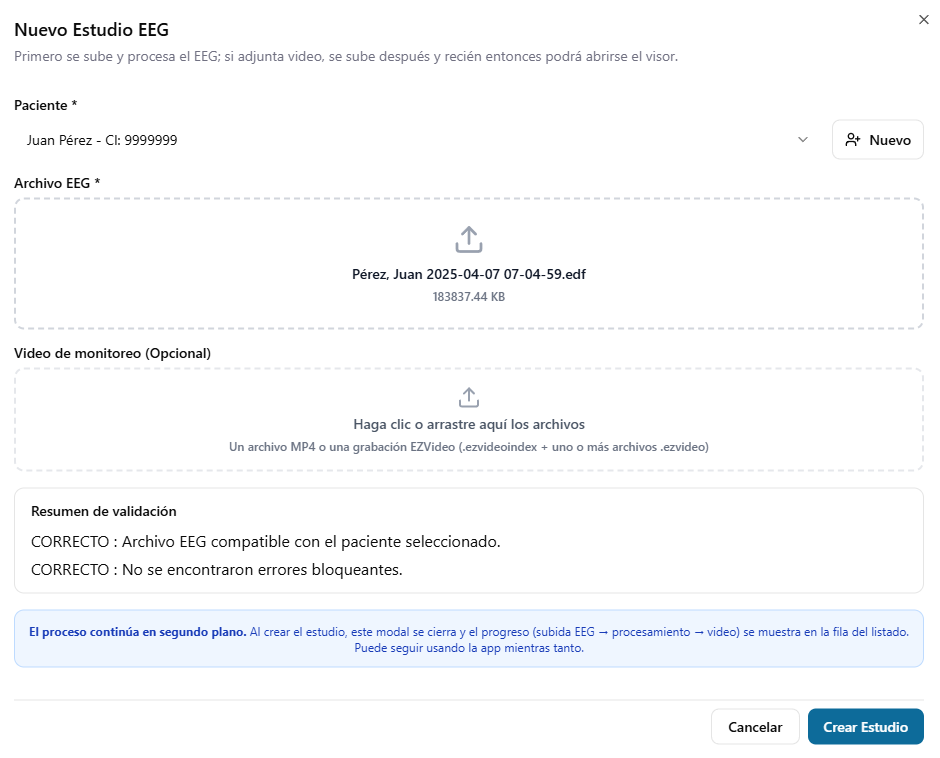
\includegraphics[
        width=0.95\textwidth,
        keepaspectratio
    ]{Chapter6/Chapter6Figs/pf04_formulario_estudio.png}

    \caption{Formulario de creación de un estudio EEG con el paciente seleccionado y el resultado de la validación del archivo.}
    \label{fig:pf04_registro_estudio}
\end{figure}


\begin{figure}[!htbp]
    \centering
    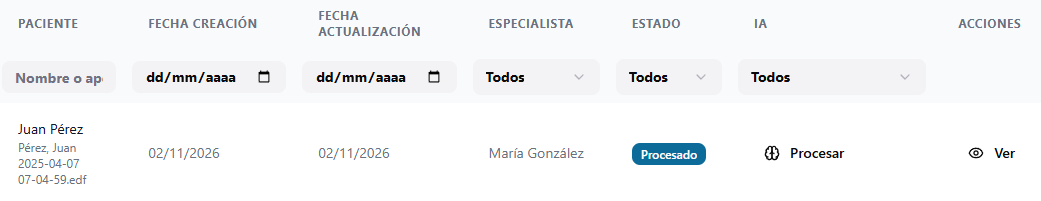
\includegraphics[
        width=0.95\textwidth,
        keepaspectratio
    ]{Chapter6/Chapter6Figs/pf04_estudio_registrado.png}

    \caption{Estudio EEG registrado y asociado al paciente Juan Pérez, con estado Procesado.}
    \label{fig:pf04_estudio_registrado}
\end{figure}

\FloatBarrier

\subsection{Resultados de la prueba de visualización de señales EEG}

La prueba funcional PF-06 tuvo como objetivo verificar la representación gráfica de las señales electroencefalográficas y la identificación de sus canales correspondientes en el visualizador de EpilexIA.

Para ejecutar la prueba, se seleccionó un estudio EEG previamente registrado y procesado en la plataforma. Posteriormente, se accedió al visualizador y se configuró el montaje Doble Banana, utilizando una ventana temporal de 10 segundos. El registro empleado tiene una frecuencia de muestreo de 250~Hz.

Durante la evaluación, se comprobó que el sistema representaba las señales electroencefalográficas mediante trazados individuales, identificados con sus respectivas derivaciones. Asimismo, se observaron las referencias temporales y la escala de amplitud utilizadas para facilitar la interpretación visual de los registros.

Como parte de la verificación, se modificó el parámetro de sensibilidad del visualizador. Inicialmente, se utilizó un valor de 100~$\mu$V, con el cual las variaciones de las señales presentaban una amplitud visual reducida. Posteriormente, se configuró una sensibilidad de 5~$\mu$V, lo que permitió observar las oscilaciones con mayor detalle.

Las Figuras~\ref{fig:pf06_sensibilidad_100} y
\ref{fig:pf06_sensibilidad_5} presentan
la representación de las señales EEG
con diferentes configuraciones de sensibilidad,
aplicadas sobre el mismo intervalo del estudio.

Los resultados observados coincidieron con el comportamiento esperado para el caso PF-06, por lo que la prueba se clasificó como aprobada. La evaluación permitió verificar la representación gráfica de las señales, la identificación de sus canales y la visualización de las referencias temporales. La comprobación específica de los montajes y de los parámetros de filtrado se contempla en los casos PF-07 y PF-08, respectivamente.


\begin{figure}[!htbp]
    \centering
    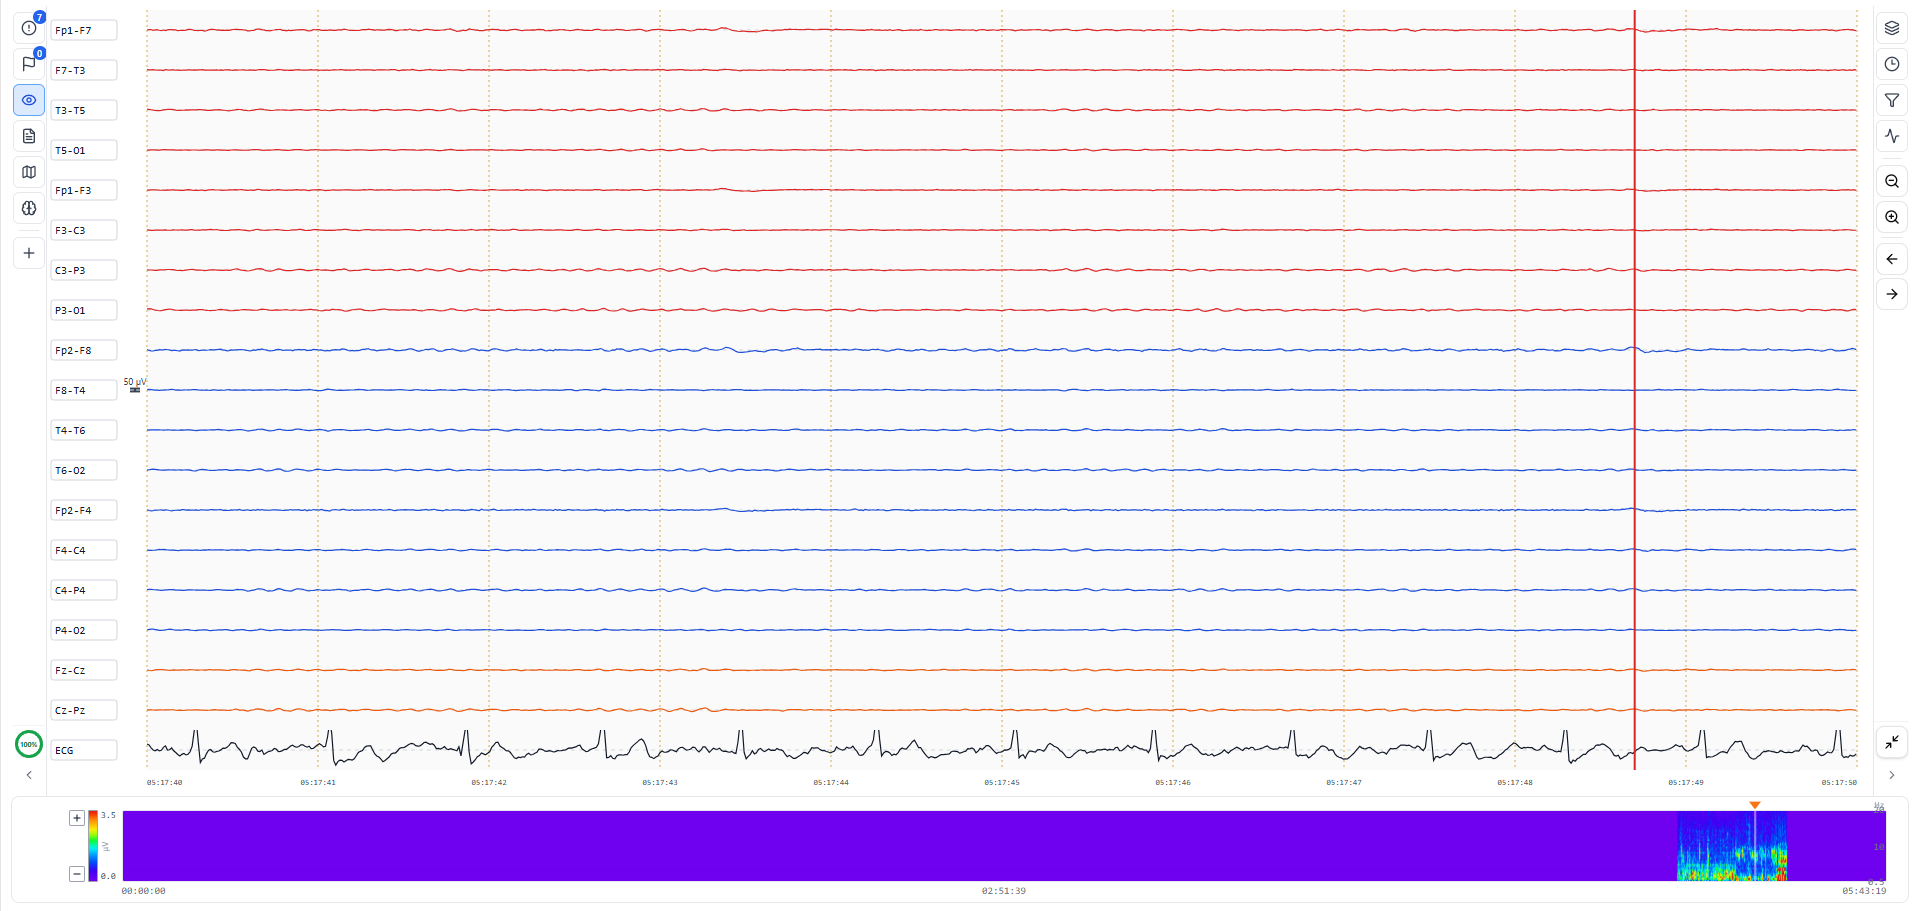
\includegraphics[
        width=\textwidth,
        height=0.65\textheight,
        keepaspectratio
    ]{Chapter6/Chapter6Figs/pf06_eeg_sensibilidad_100uv.png}

    \caption{Visualización de señales EEG en EpilexIA con sensibilidad de 100~$\mu$V.}
    \label{fig:pf06_sensibilidad_100}
\end{figure}

\begin{figure}[!t]
    \centering
    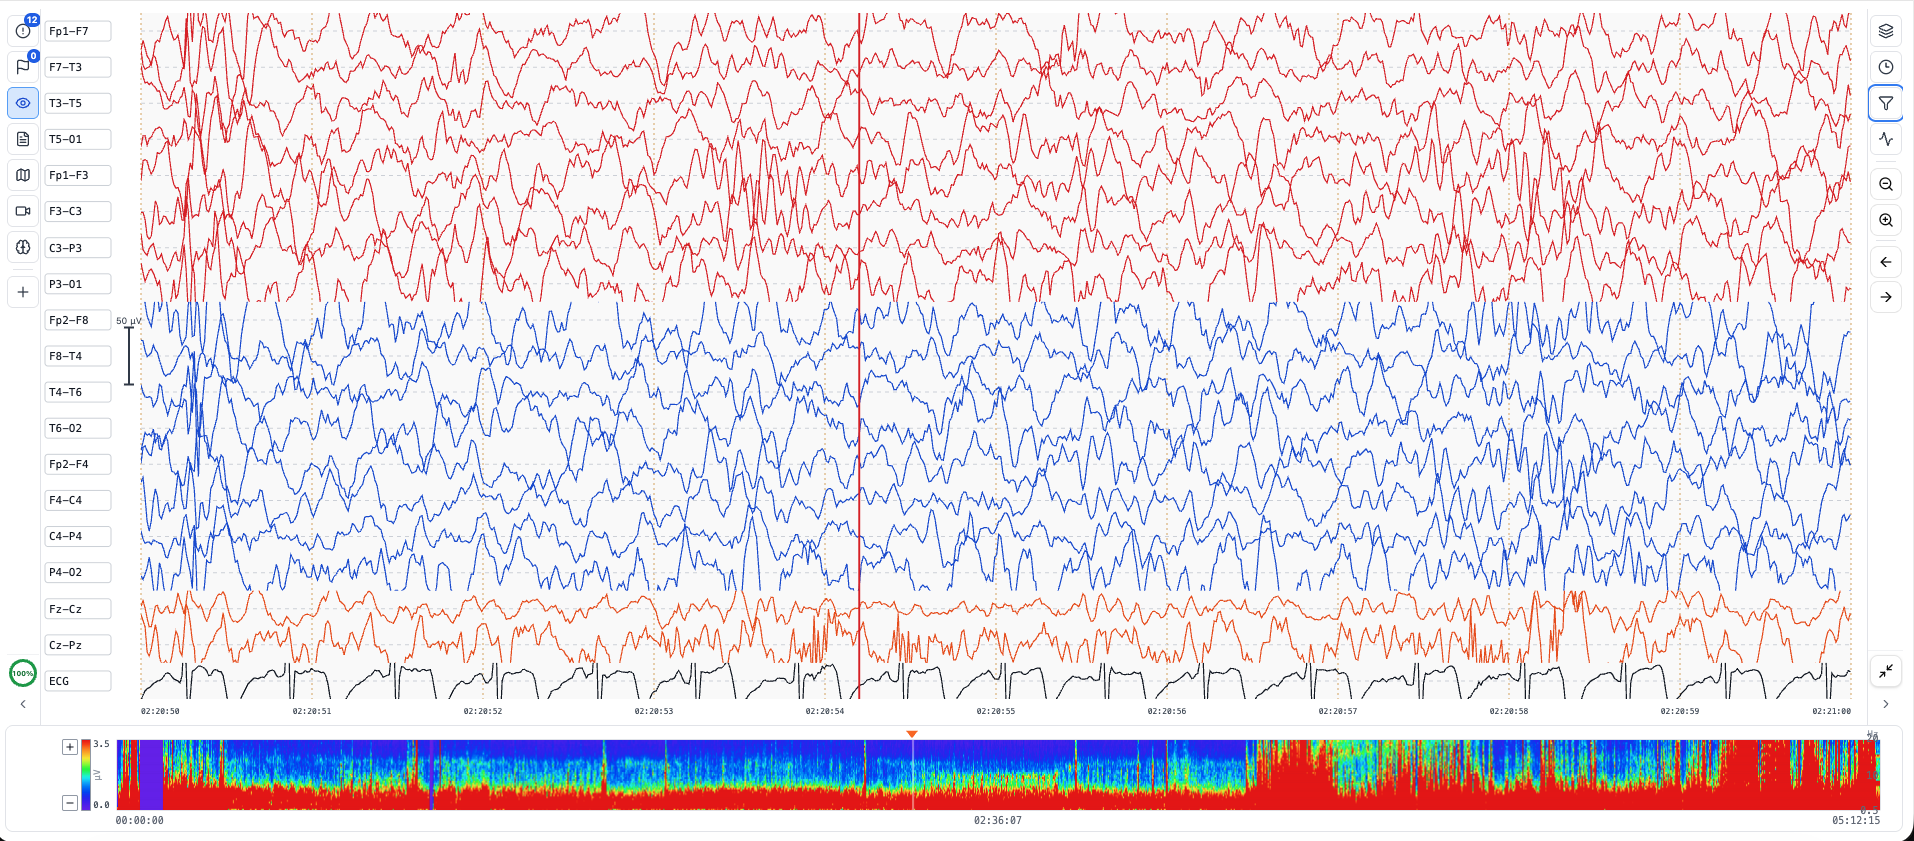
\includegraphics[
        width=\textwidth,
        height=0.65\textheight,
        keepaspectratio
    ]{Chapter6/Chapter6Figs/pf06_eeg_sensibilidad_5uv.png}

    \caption{Visualización de señales EEG en EpilexIA con sensibilidad de 5~$\mu$V.}
    \label{fig:pf06_sensibilidad_5}
\end{figure}

\FloatBarrier


\subsection{Resultados de la prueba de configuración de montajes EEG}

La prueba funcional PF-07 tuvo como objetivo verificar que el visualizador de EpilexIA permitiera seleccionar diferentes montajes electroencefalográficos y representar las señales de acuerdo con la configuración seleccionada.

Para ejecutar la prueba, se utilizó un estudio EEG previamente registrado y procesado en la plataforma. Se accedió al visualizador y se seleccionó inicialmente el montaje Doble Banana, utilizando una ventana temporal de 10 segundos. Posteriormente, se cambió al montaje Transversal, manteniendo el mismo intervalo del registro para facilitar la comparación.

Durante la evaluación, se observó que el montaje Doble Banana presentaba las señales mediante derivaciones longitudinales, entre ellas Fp1-F7, F7-T3, T3-T5 y Fp2-F8. Estas derivaciones se encontraban identificadas mediante sus respectivas etiquetas dentro del área de visualización.

Al seleccionar el montaje Transversal, el sistema actualizó la disposición de los trazados y presentó un conjunto diferente de derivaciones, entre ellas Fp1-Fp2, F3-Fz, C3-Cz y Cz-C4. El cambio permitió comprobar que la representación gráfica respondía a la configuración seleccionada por el usuario.

Las Figuras~\ref{fig:pf07_doble_banana} y~\ref{fig:pf07_transversal} presentan las señales electroencefalográficas correspondientes a ambos montajes, utilizando el mismo intervalo temporal del estudio.

Los resultados observados coincidieron con el comportamiento esperado para el caso PF-07, por lo que la prueba se clasificó como aprobada. La evaluación permitió verificar la selección de montajes disponibles, la actualización de las derivaciones representadas y la conservación de las referencias temporales durante el cambio de configuración. La prueba se limitó a comprobar el comportamiento funcional del visualizador, sin incluir una validación clínica de las señales representadas.


\begin{figure}[p]
    \centering
    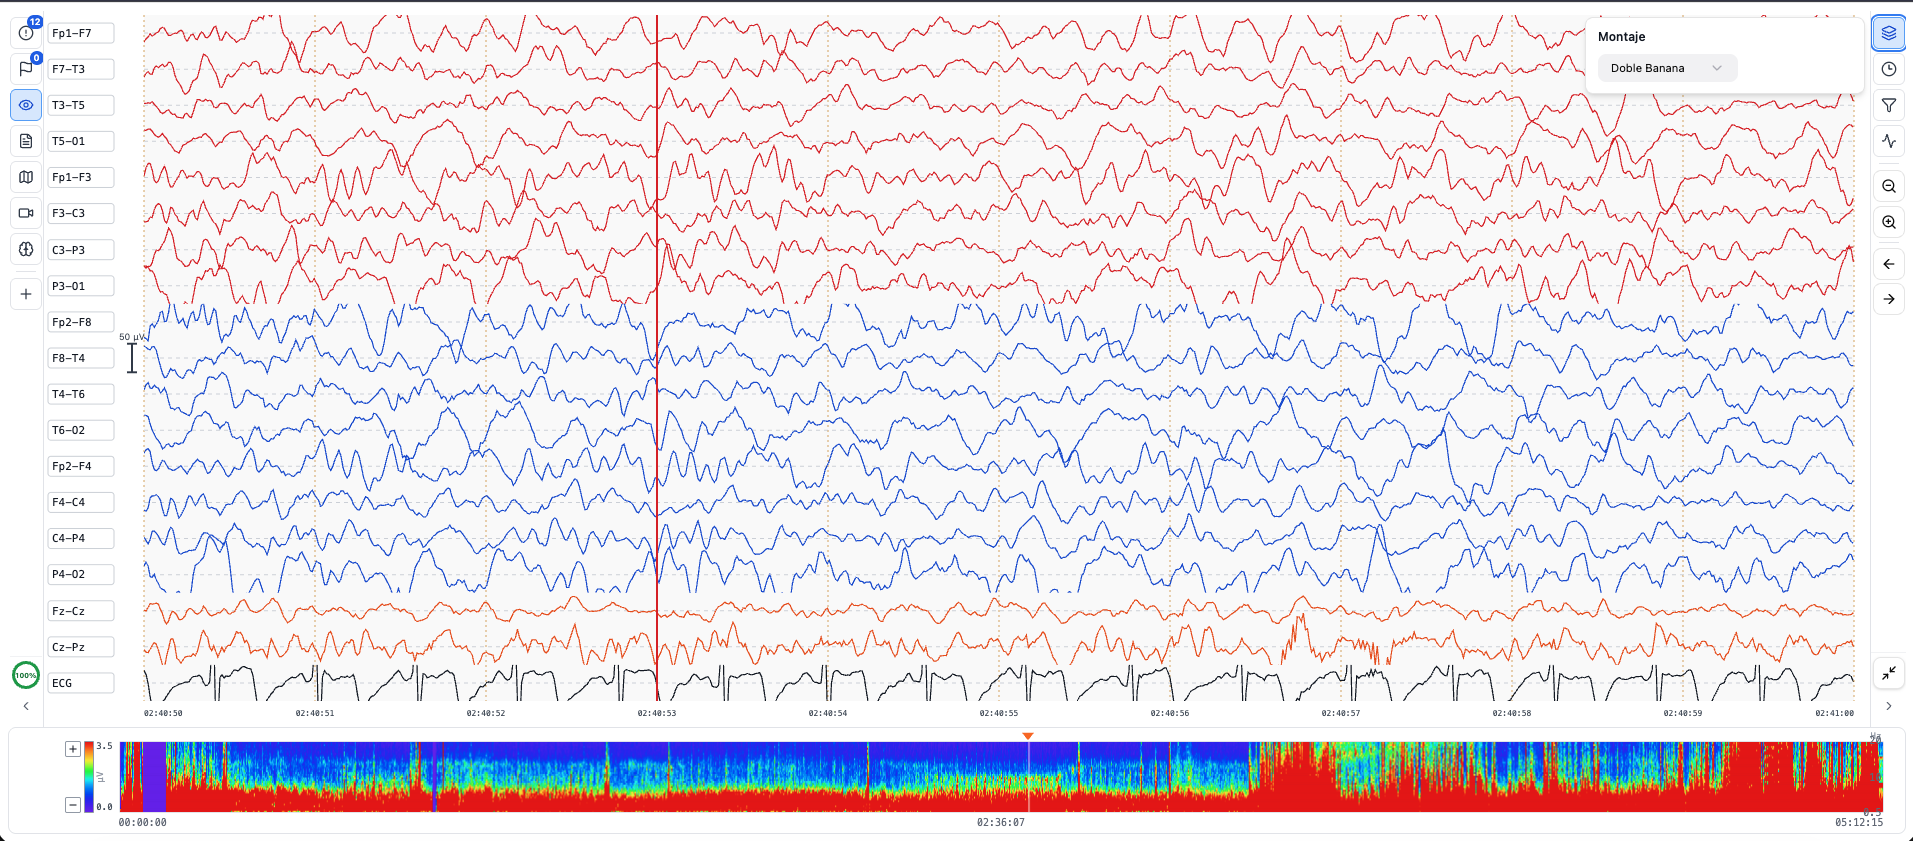
\includegraphics[width=0.95\textwidth]{Chapter6/Chapter6Figs/pf07_montaje_doble_banana.png}
    \caption{Visualización de señales electroencefalográficas en EpilexIA utilizando el montaje Doble Banana.}
    \label{fig:pf07_doble_banana}
\end{figure}

\begin{figure}[p]
    \centering
    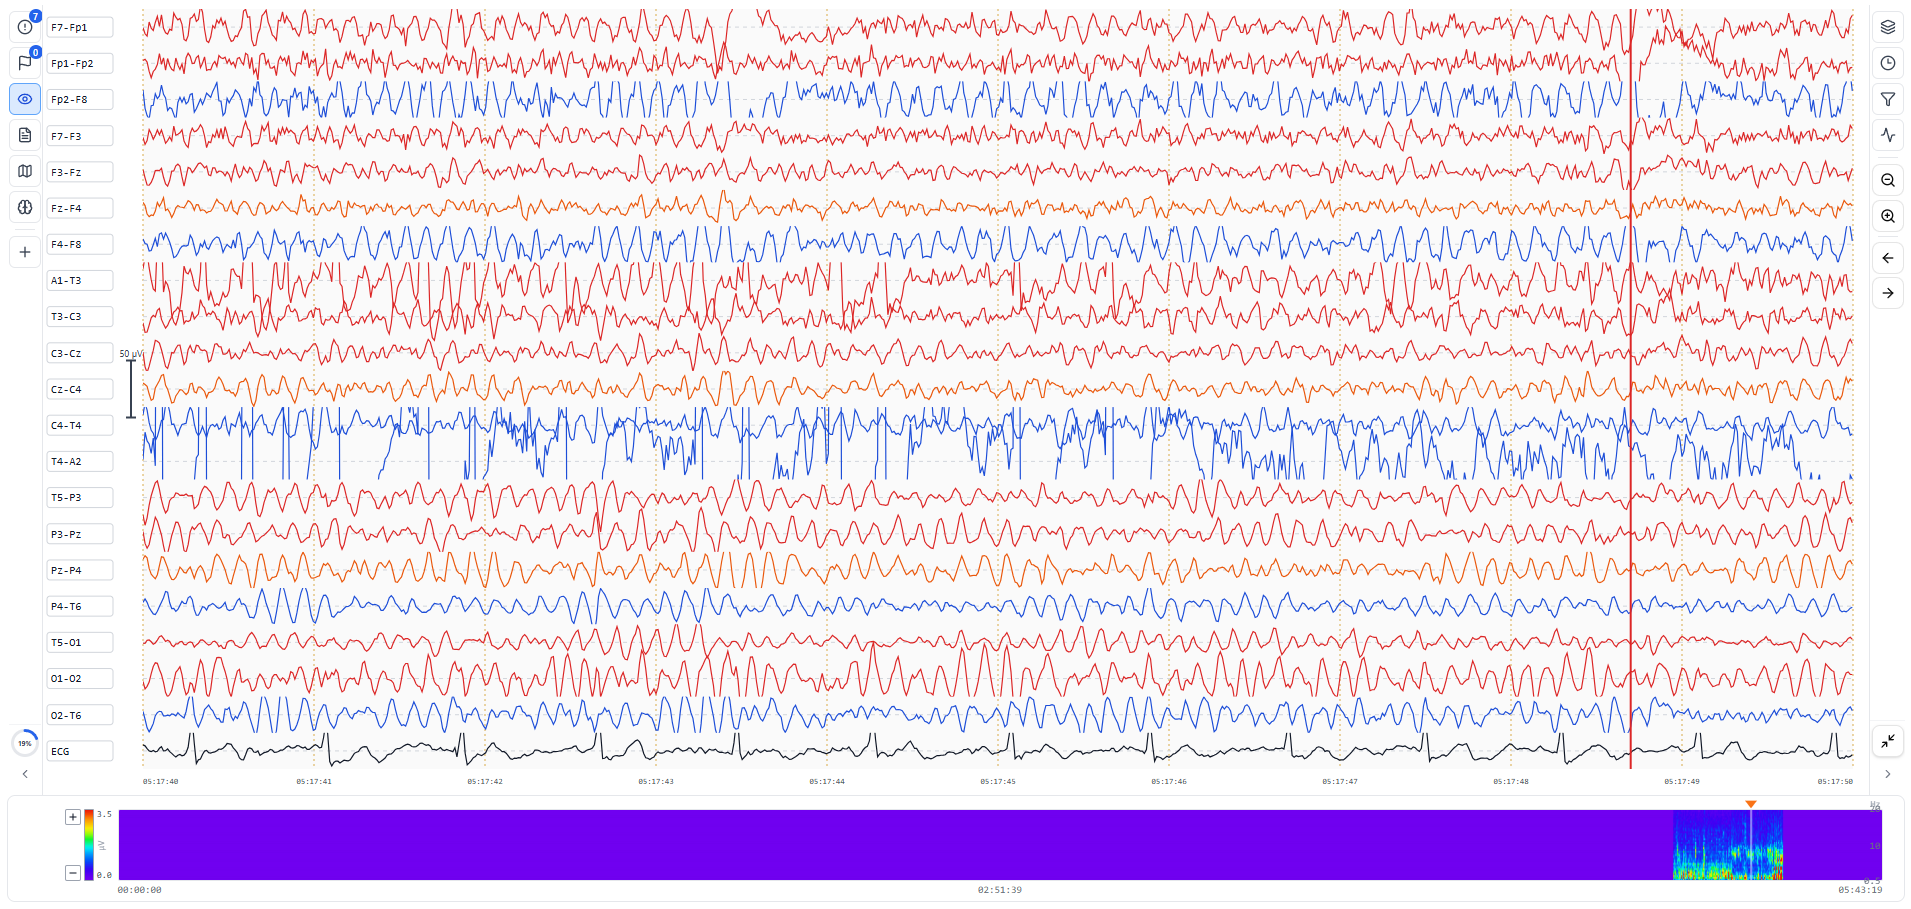
\includegraphics[width=0.95\textwidth]{Chapter6/Chapter6Figs/pf07_montaje_transversal.png}
    \caption{Visualización de señales electroencefalográficas en EpilexIA utilizando el montaje Transversal.}
    \label{fig:pf07_transversal}
\end{figure}

\FloatBarrier


\subsection{Resultados de la prueba de configuración de filtros EEG}

La prueba funcional PF-08 tuvo como objetivo verificar que el visualizador de EpilexIA permitiera modificar los parámetros de filtrado de las señales electroencefalográficas y observar los cambios producidos en su representación gráfica.

Para ejecutar la prueba, se utilizó un estudio EEG previamente registrado y procesado en la plataforma. Se accedió al visualizador y se seleccionó el montaje Doble Banana, utilizando una ventana temporal de 10 segundos y una sensibilidad de 10~$\mu$V. Cada comparación se realizó sobre un mismo intervalo del registro.

Inicialmente, se evaluó el filtro de corte inferior (\textit{Low cut}), configurando valores de 1 Hz y 0,5 Hz, mientras se mantuvo el filtro de corte superior en 70 Hz. Al modificar este parámetro, se observaron diferencias en la representación de determinadas derivaciones, particularmente en los componentes de baja frecuencia, que se aprecian con mayor amplitud al reducir la frecuencia de corte. La Figura~\ref{fig:pf08_lowcut} presenta las configuraciones evaluadas.
Posteriormente, se evaluó el filtro de corte superior (\textit{High cut}), utilizando valores de 70 Hz y 30 Hz, con el filtro de corte inferior establecido en 1 Hz. Durante la comparación, se observaron modificaciones en la forma de algunos trazados, compatibles con la atenuación de componentes de mayor frecuencia. La Figura~\ref{fig:pf08_highcut} muestra los resultados obtenidos.

Finalmente, se evaluó el filtro de rechazo de banda (\textit{Notch}) de 50 Hz, mediante su activación y desactivación. Con el filtro desactivado se observó una interferencia de alta frecuencia superpuesta a las señales, especialmente notoria en las derivaciones F3-C3, C3-P3 y Fz-Cz, que dejó de apreciarse al activarlo. La Figura~\ref{fig:pf08_notch} presenta ambas configuraciones.

Los resultados observados fueron compatibles con el comportamiento esperado para el caso PF-08, por lo que la comprobación funcional visual se clasificó como aprobada. La evaluación permitió verificar la modificación de los parámetros de filtrado y los cambios correspondientes en la representación de las señales EEG. La prueba se limitó a la verificación funcional del visualizador, sin incluir mediciones cuantitativas de la respuesta frecuencial de los filtros ni una validación clínica de las señales representadas.


\begin{figure}[p]
    \centering
    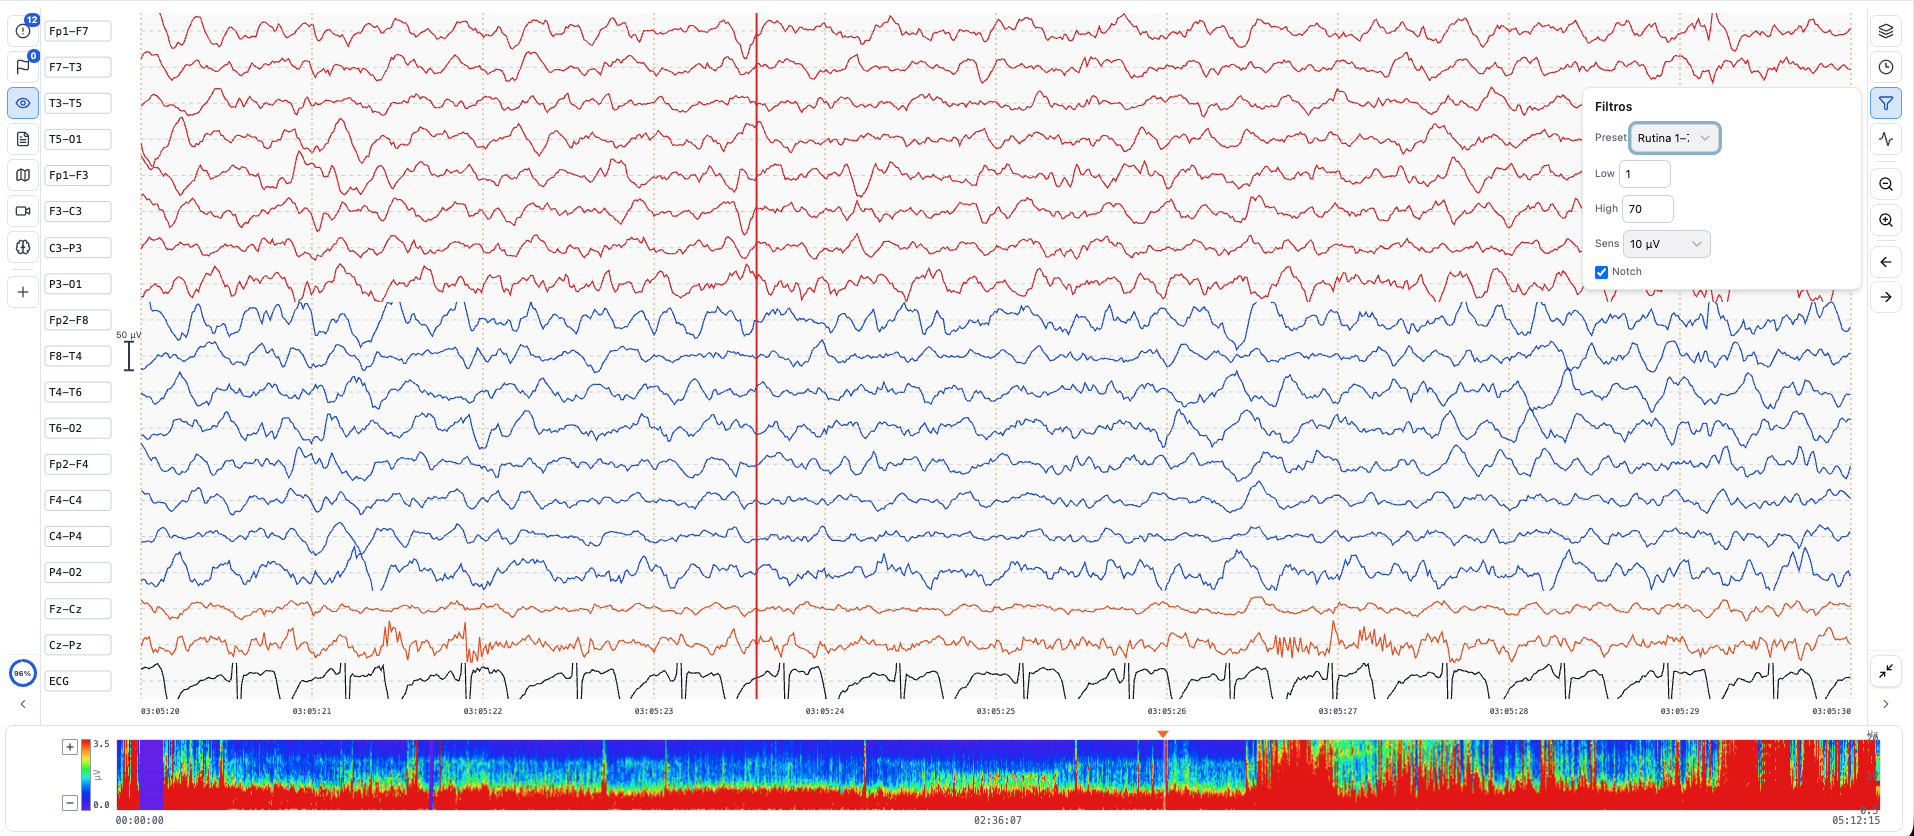
\includegraphics[width=0.85\textwidth]{Chapter6/Chapter6Figs/pf08_lowcut_1hz.png}

    \par\smallskip
    {\small (a) Señales EEG con Low cut de 1 Hz.}

    \vspace{0.4cm}

    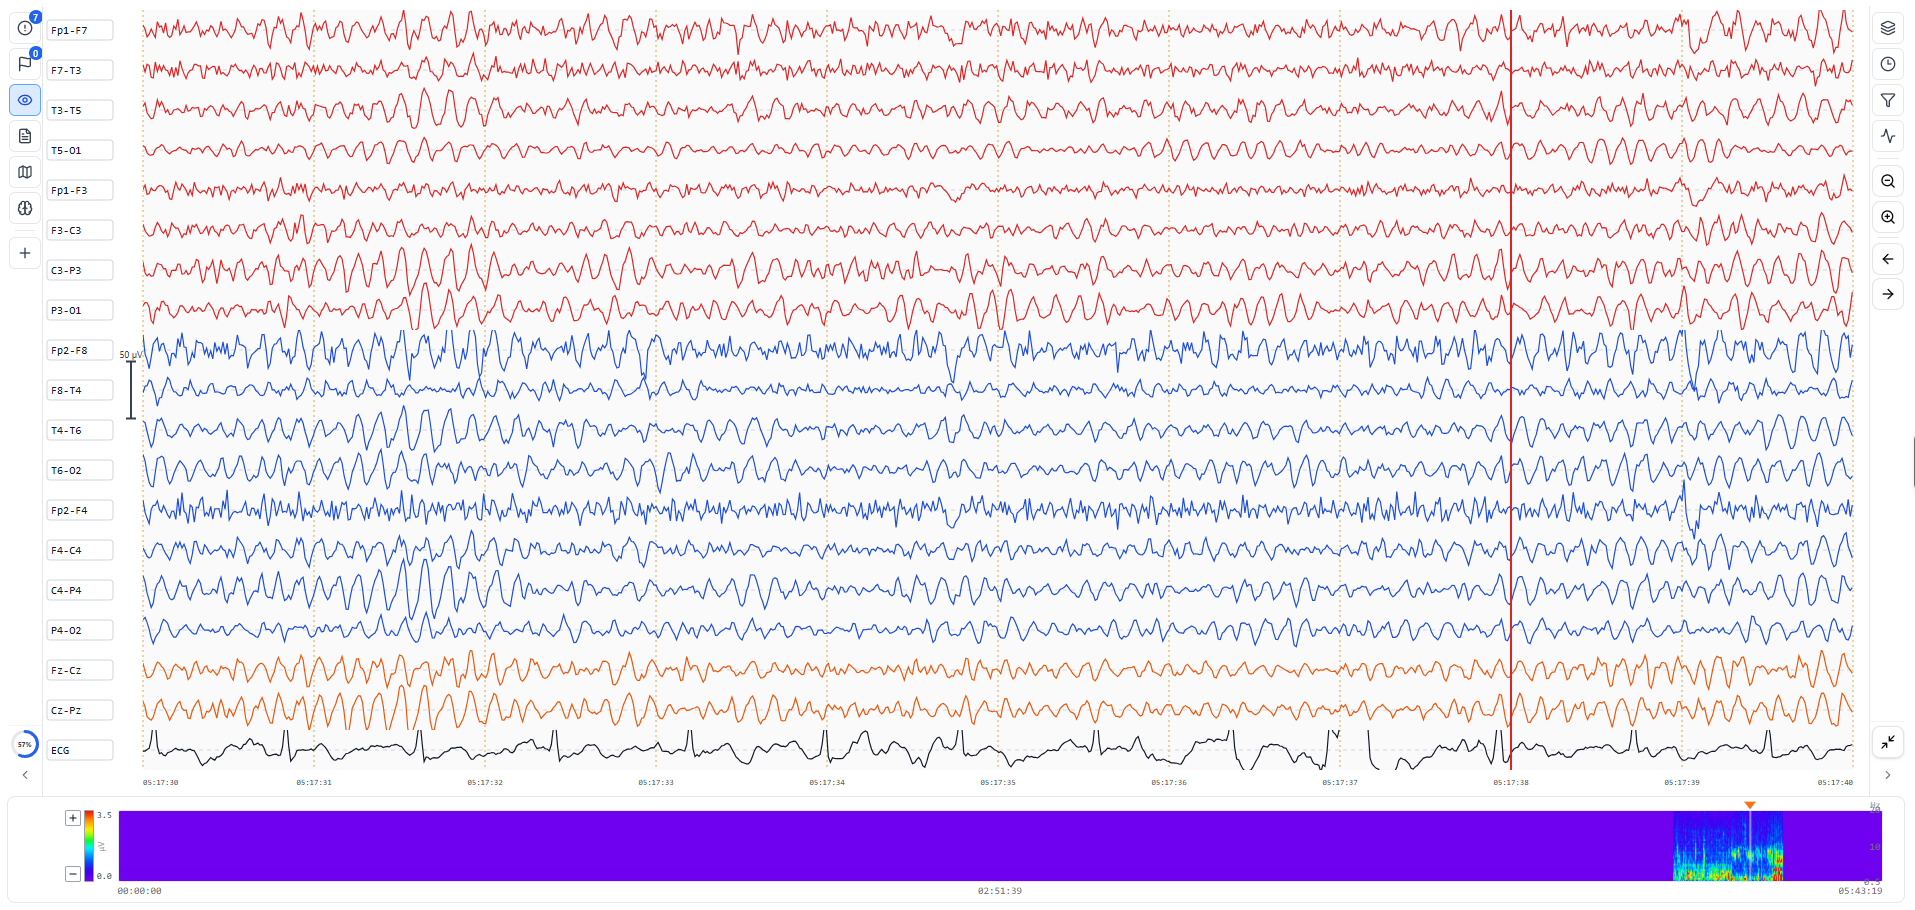
\includegraphics[width=0.85\textwidth]{Chapter6/Chapter6Figs/pf08_lowcut_5hz.png}

    \par\smallskip
    {\small (b) Señales EEG con Low cut de 0,5 Hz.}

    \caption{Comparación de señales EEG con diferentes configuraciones del filtro de corte inferior.}
    \label{fig:pf08_lowcut}
\end{figure}


\begin{figure}[p]
    \centering
    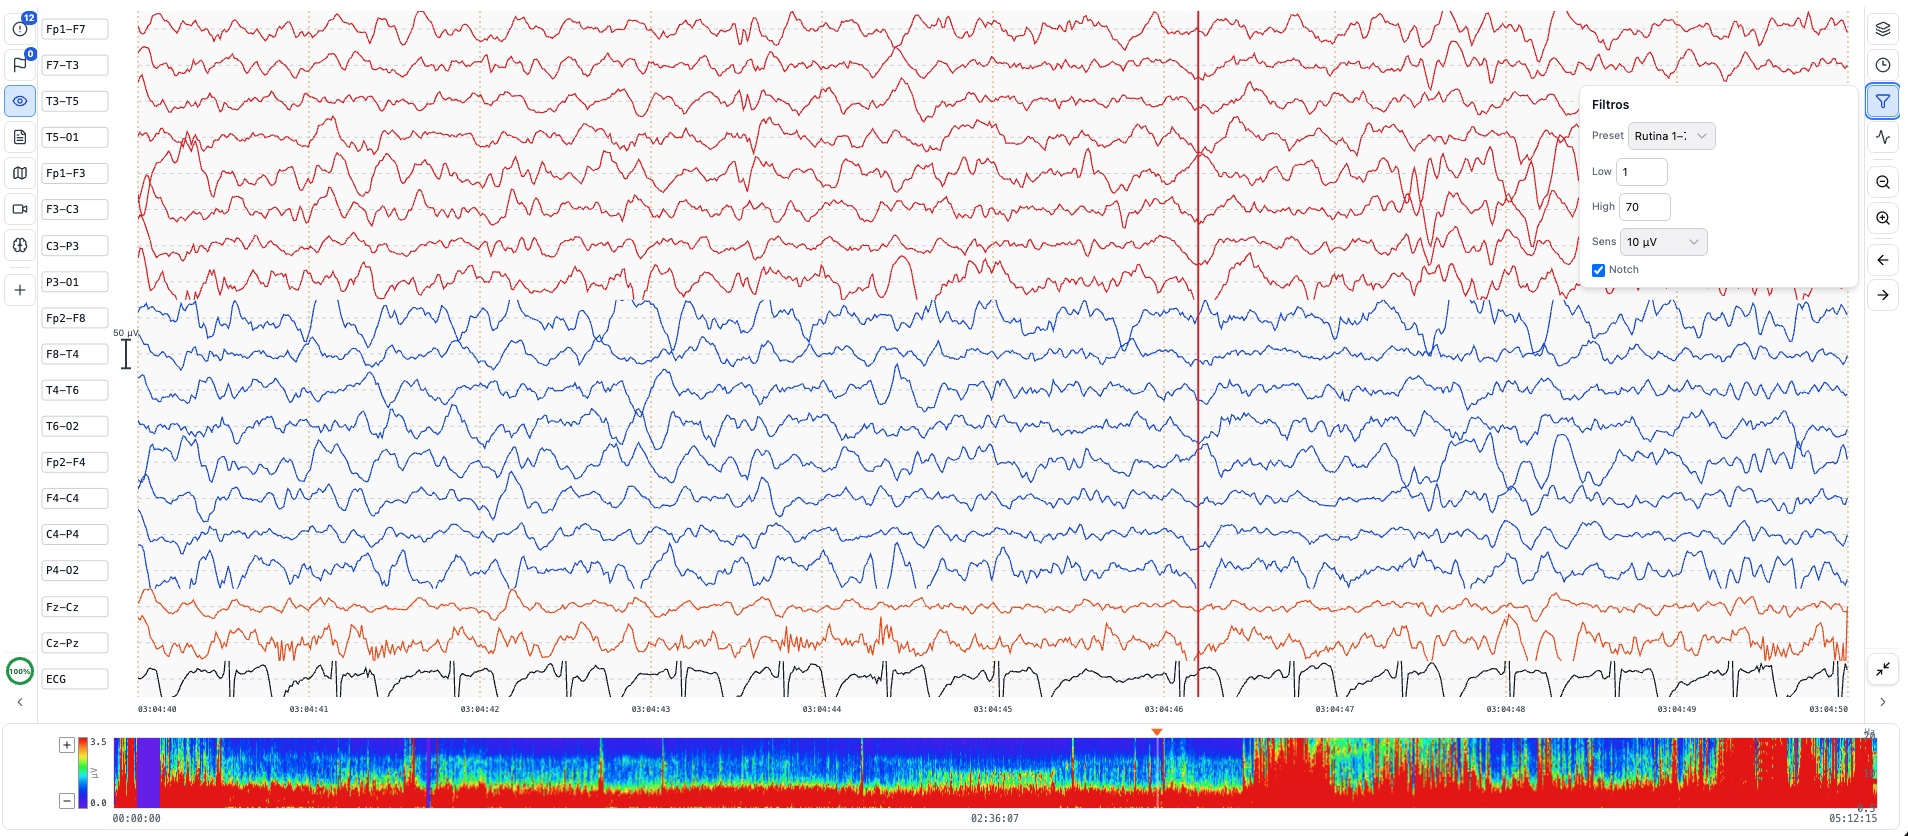
\includegraphics[width=0.85\textwidth]{Chapter6/Chapter6Figs/pf08_highcut_70hz.png}

    \par\smallskip
    {\small (a) Señales EEG con High cut de 70 Hz.}

    \vspace{0.4cm}

    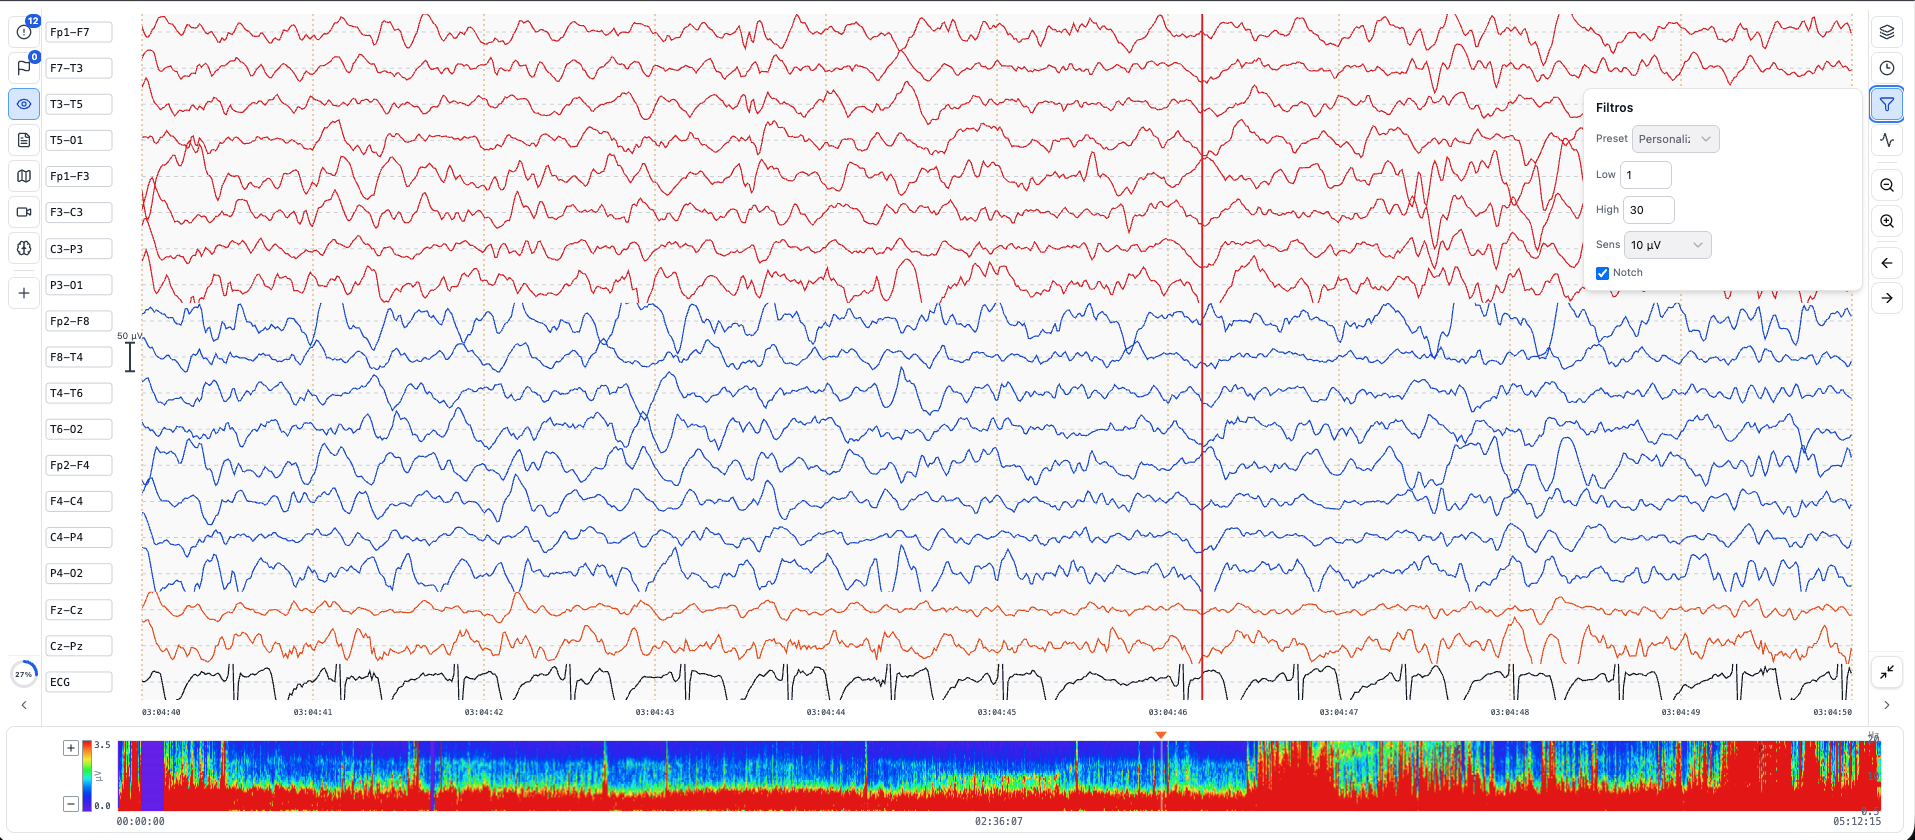
\includegraphics[width=0.85\textwidth]{Chapter6/Chapter6Figs/pf08_highcut_30hz.png}

    \par\smallskip
    {\small (b) Señales EEG con High cut de 30 Hz.}

    \caption{Comparación de señales EEG con diferentes configuraciones del filtro de corte superior.}
    \label{fig:pf08_highcut}
\end{figure}


\begin{figure}[p]
    \centering
    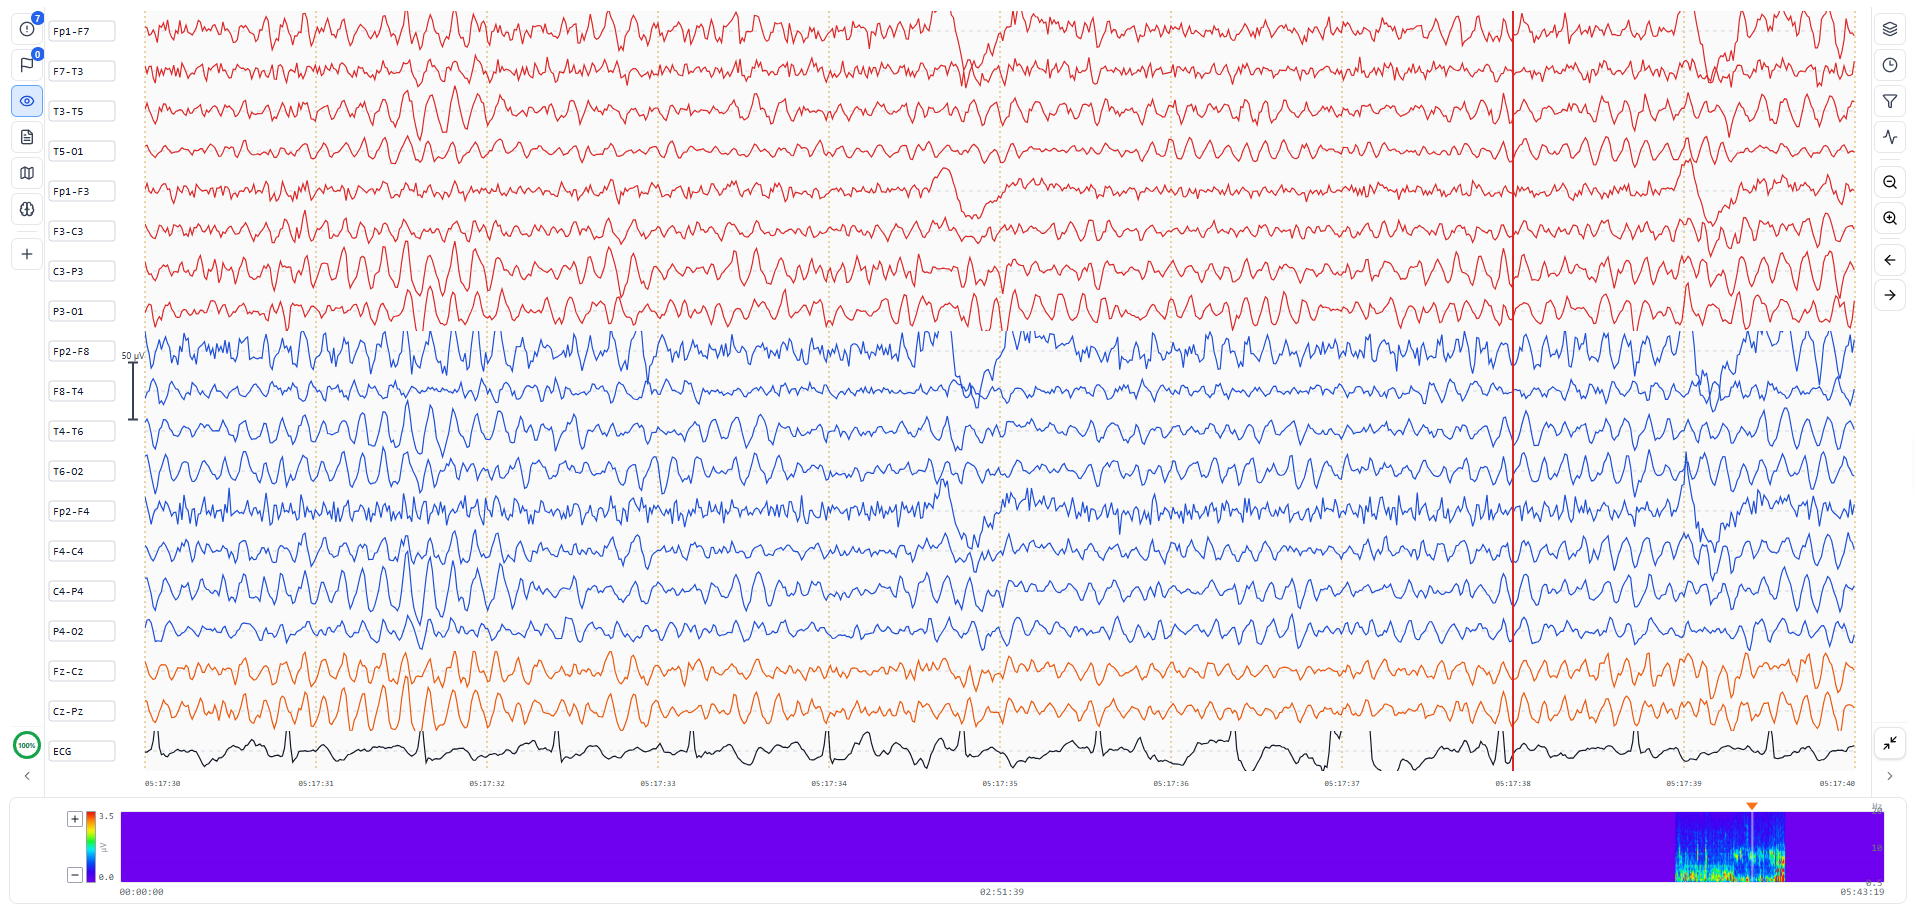
\includegraphics[width=0.85\textwidth]{Chapter6/Chapter6Figs/pf08_notch_activado.png}

    \par\smallskip
    {\small (a) Señales EEG con Notch de 50 Hz activado.}

    \vspace{0.4cm}

    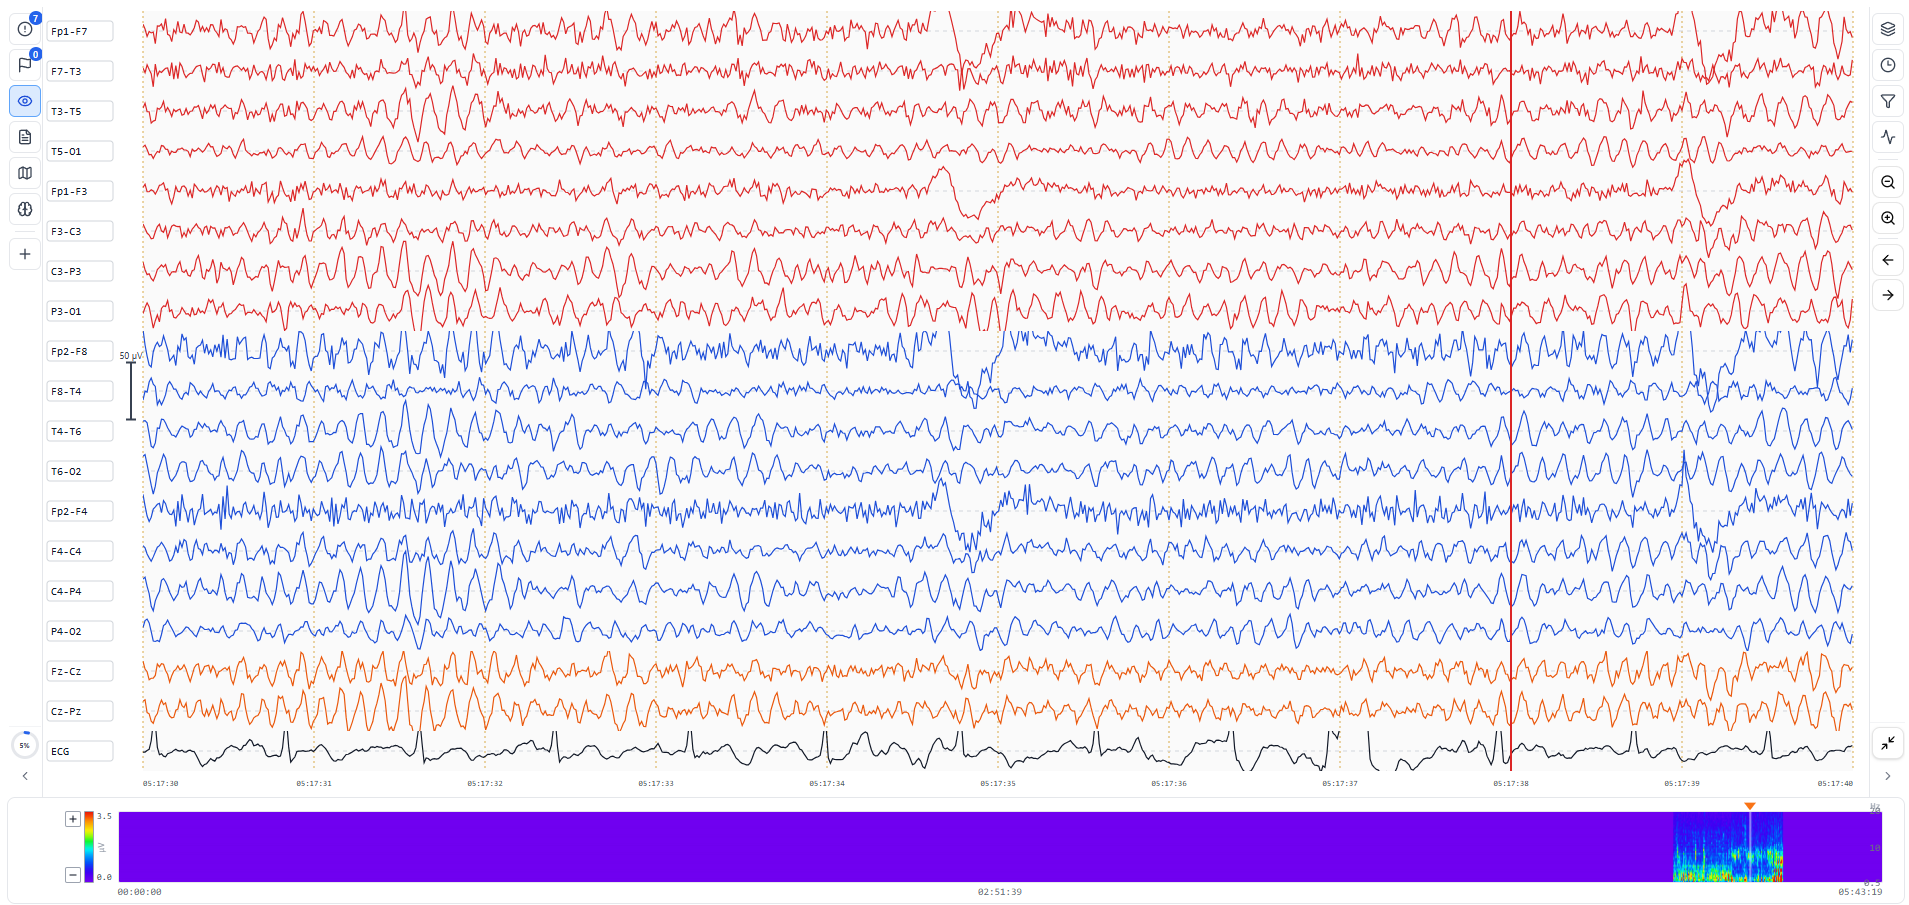
\includegraphics[width=0.85\textwidth]{Chapter6/Chapter6Figs/pf08_notch_desactivado.png}

    \par\smallskip
    {\small (b) Señales EEG con Notch de 50 Hz desactivado.}

    \caption{Comparación de señales EEG con el filtro Notch de 50 Hz activado y desactivado.}
    \label{fig:pf08_notch}
\end{figure}

\FloatBarrier


\subsection[Resultados de la prueba de registro manual de anomalías]{Resultados de la prueba de registro manual de \\anomalías}

La prueba funcional PF-09 tuvo como objetivo verificar que EpilexIA permitiera registrar manualmente anomalías durante la visualización de señales electroencefalográficas, asociándolas al estudio EEG y al intervalo temporal seleccionado.

Para ejecutar la prueba, se accedió a un estudio EEG previamente registrado y procesado en la plataforma. Se utilizó el montaje Doble Banana, con una ventana temporal de 10 segundos. El registro empleado tiene una frecuencia de muestreo de 250~Hz.

Posteriormente, se activó la funcionalidad de marcado manual y se seleccionó un intervalo comprendido entre los instantes 03:03:50 y 03:03:59 del registro, correspondiente a una duración de nueve segundos. El sistema resaltó gráficamente el intervalo seleccionado y presentó la opción para guardar el registro como anomalía.

La Figura~\ref{fig:pf09_seleccion_anomalia} muestra la selección temporal realizada sobre las señales EEG.

Una vez confirmada la operación, se verificó que la anomalía apareciera identificada como un registro manual, conservando las referencias temporales correspondientes al intervalo seleccionado.


Asimismo, se comprobó que la anomalía registrada se encontraba disponible en el apartado de registro de anomalías del informe médico asociado al estudio, tal como se observa en la Figura~\ref{fig:pf09_anomalia_registrada}.

Adicionalmente, se realizó una comprobación de persistencia del registro. Para ello, se cerró la sesión del usuario y posteriormente se volvió a acceder a la plataforma. Al consultar nuevamente el estudio EEG, se verificó que la anomalía manual permanecía disponible, conservando el intervalo temporal seleccionado.

Los resultados observados coincidieron con el comportamiento esperado para el caso PF-09, por lo que la prueba se clasificó como aprobada. La evaluación permitió verificar el registro manual de anomalías, su asociación al estudio EEG, la conservación de las referencias temporales y la persistencia de la información después de una nueva sesión.


% Figura 6.13: Selección del intervalo temporal
\begin{figure}[p]
    \centering
    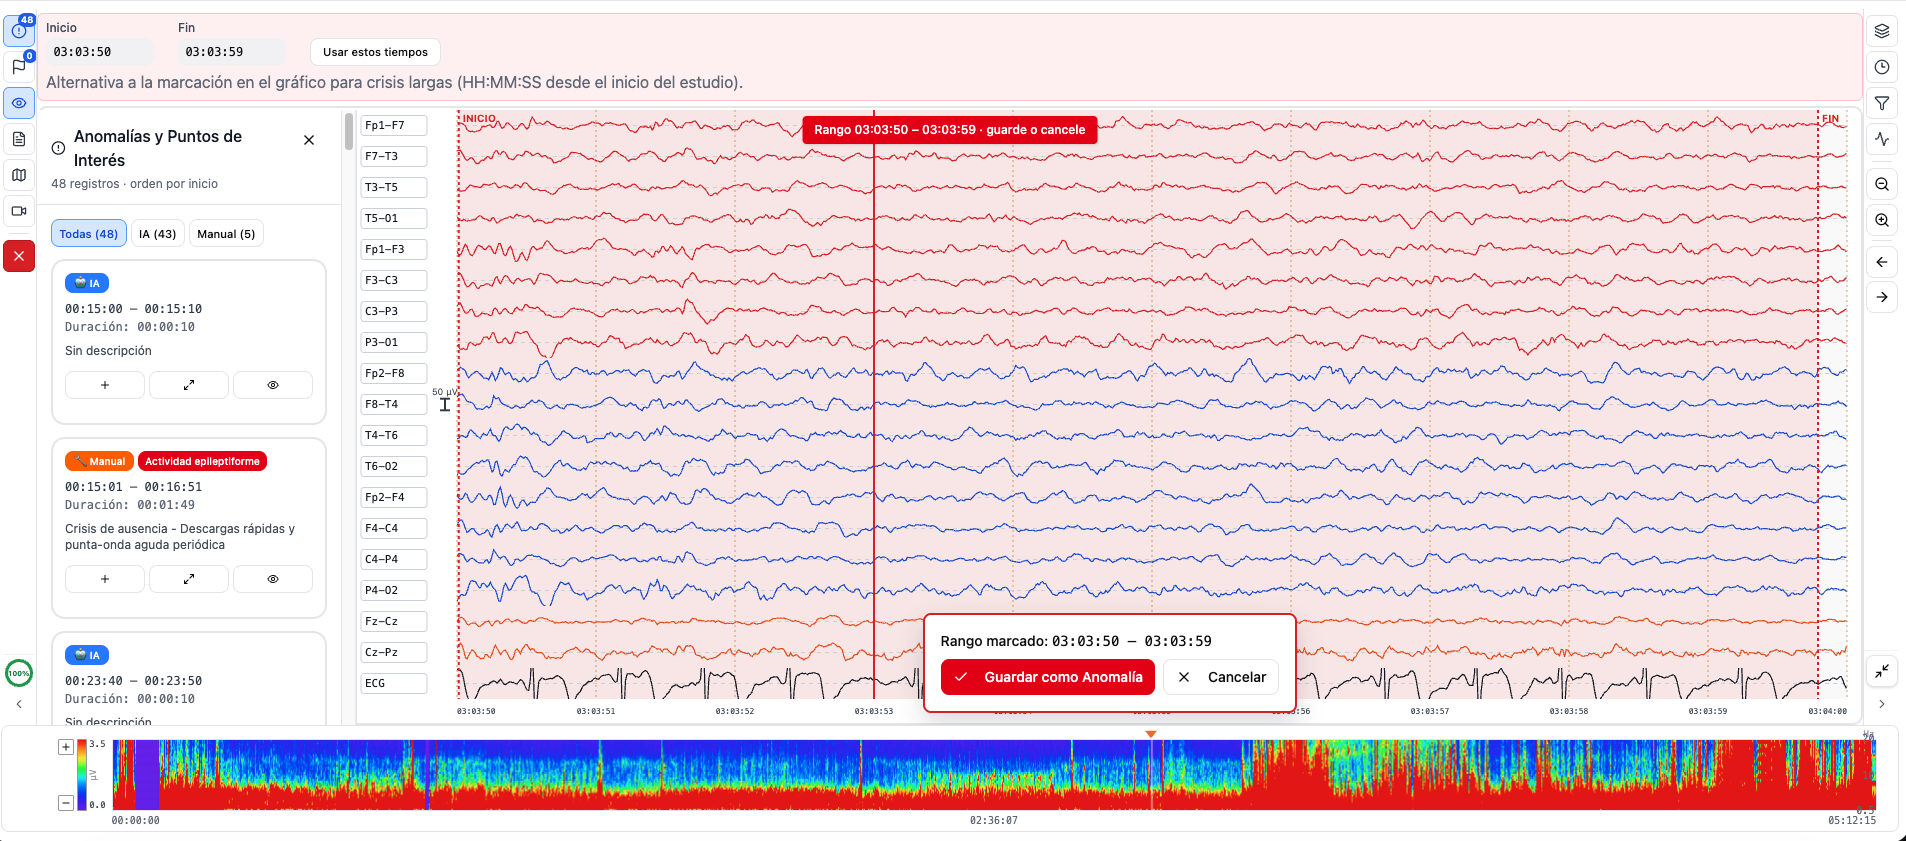
\includegraphics[width=\textwidth]{Chapter6/Chapter6Figs/pf09_seleccion_anomalia.png}
    \caption{Selección de un intervalo temporal de señales EEG para el registro manual de una anomalía en EpilexIA.}
    \label{fig:pf09_seleccion_anomalia}
\end{figure}

% Figura 6.14: Anomalía registrada
\begin{figure}[p]
    \centering
    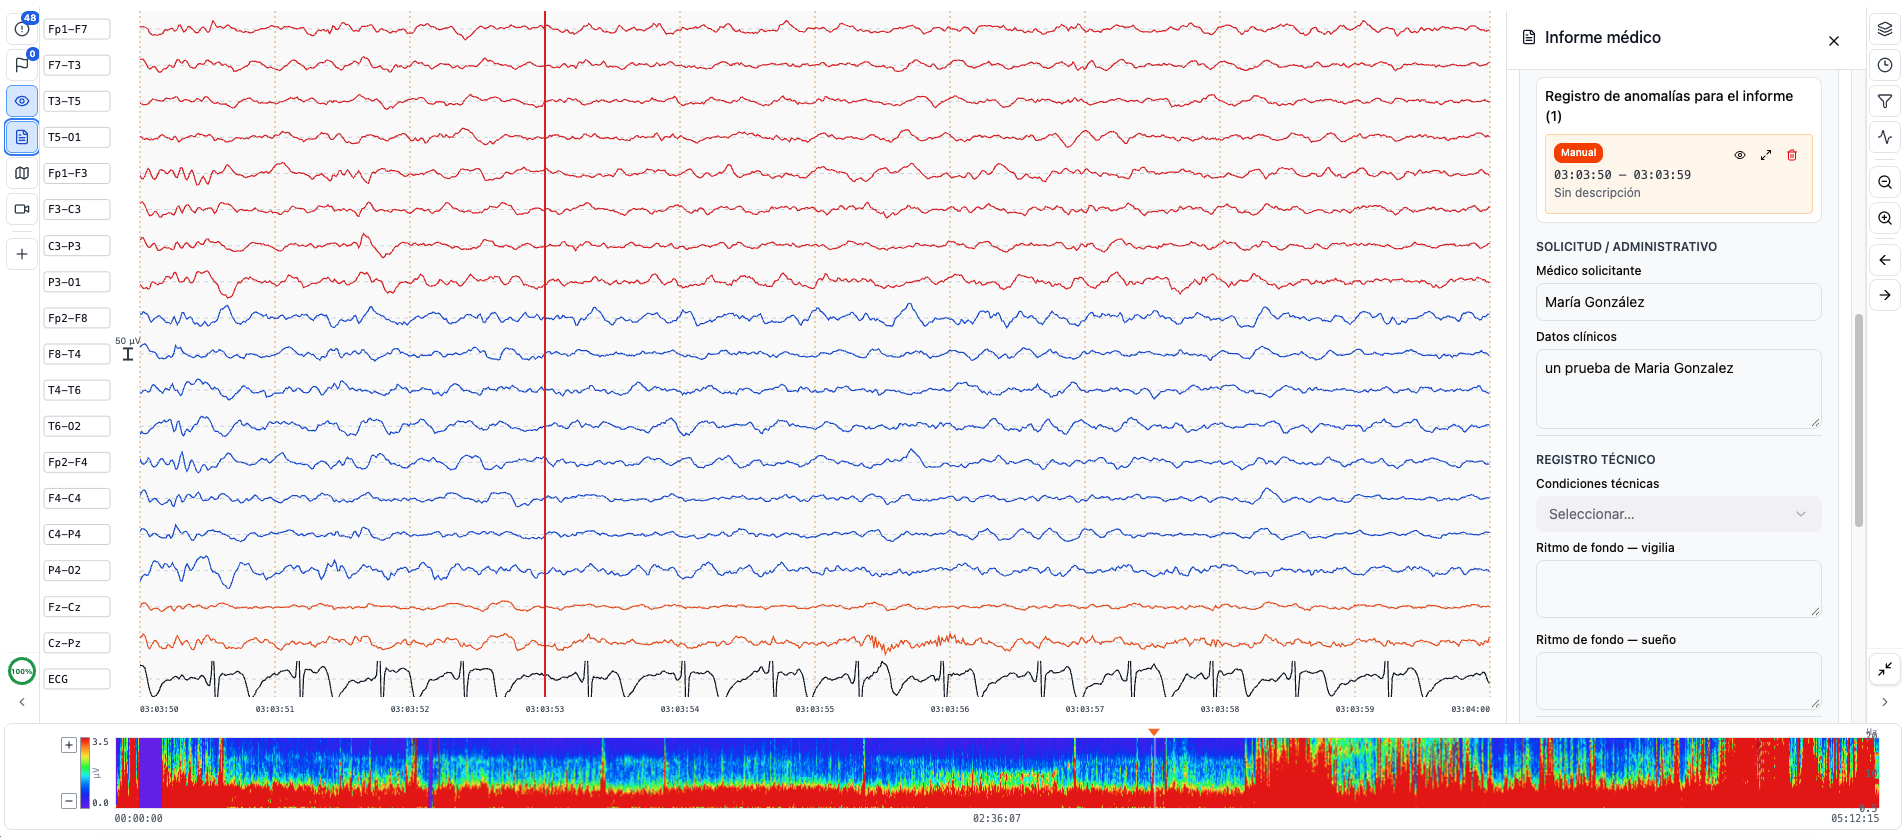
\includegraphics[width=0.95\textwidth]{Chapter6/Chapter6Figs/pf09_anomalia_registrada.png}
    \caption{Anomalía registrada manualmente y conservada en el informe médico del estudio EEG en EpilexIA.}
    \label{fig:pf09_anomalia_registrada}
\end{figure}

\FloatBarrier


\subsection{Resultados de la prueba de consulta de resultados de IA}

La prueba funcional PF-10 tuvo como objetivo verificar que EpilexIA permitiera consultar los resultados de un análisis mediante inteligencia artificial previamente finalizado, incluyendo las anomalías identificadas y sus correspondientes referencias temporales.


Para ejecutar la prueba, se utilizó un estudio EEG que contaba con resultados de inteligencia artificial previamente almacenados en la base de datos. Posteriormente, se ingresó al visualizador EEG y se consultó el apartado de anomalías y puntos de interés. Esta prueba se centró en verificar la recuperación, presentación y navegación de los resultados existentes, sin ejecutar nuevamente el motor de procesamiento de inteligencia artificial.


Durante la evaluación, se observó que el sistema presentaba un total de 47 registros, de los cuales 43 correspondían a anomalías identificadas mediante inteligencia artificial y 4 a registros manuales. Asimismo, se comprobó que los registros podían distinguirse según su origen mediante las opciones de filtrado disponibles en el panel.


La Figura~\ref{fig:pf10_resultados_ia} presenta el listado de anomalías identificadas mediante inteligencia artificial y su visualización dentro del estudio EEG.

Posteriormente, se seleccionó una anomalía identificada mediante IA, correspondiente al intervalo comprendido entre los instantes 01:43:10 y 01:43:20 del registro, con una duración de 10 segundos. Esta duración corresponde a una ventana de análisis, dado que los resultados del modelo se almacenan por ventana (Sección~\ref{subsec:modelo-vigente-hgb}). Al utilizar la opción de consulta de detalles, el sistema presentó una ventana con las referencias temporales del registro y los campos disponibles para su descripción y clasificación, tal como se observa en la Figura~\ref{fig:pf10_detalle_ia}.

Adicionalmente, se comprobó que, mediante la opción de visualización identificada con el icono de un ojo, el sistema permitía navegar directamente al intervalo temporal correspondiente a la anomalía seleccionada. Una vez localizado el intervalo, el visualizador resaltó gráficamente la región mediante un sombreado, facilitando su identificación dentro de las señales EEG, como se observa en la Figura~\ref{fig:pf10_intervalo_ia}.

Los resultados observados coincidieron con el comportamiento esperado para el caso PF-10, por lo que la prueba se clasificó como aprobada. La evaluación permitió verificar la disponibilidad de los resultados del análisis mediante IA, la identificación de los registros según su origen, la consulta de sus referencias temporales y la navegación hacia los intervalos correspondientes dentro del estudio EEG. La prueba se limitó a comprobar el comportamiento funcional de la plataforma, sin incluir una evaluación de la precisión diagnóstica del modelo de inteligencia artificial.


% Figura 6.15 - Resultados de IA
\begin{figure}[htbp]
    \centering
    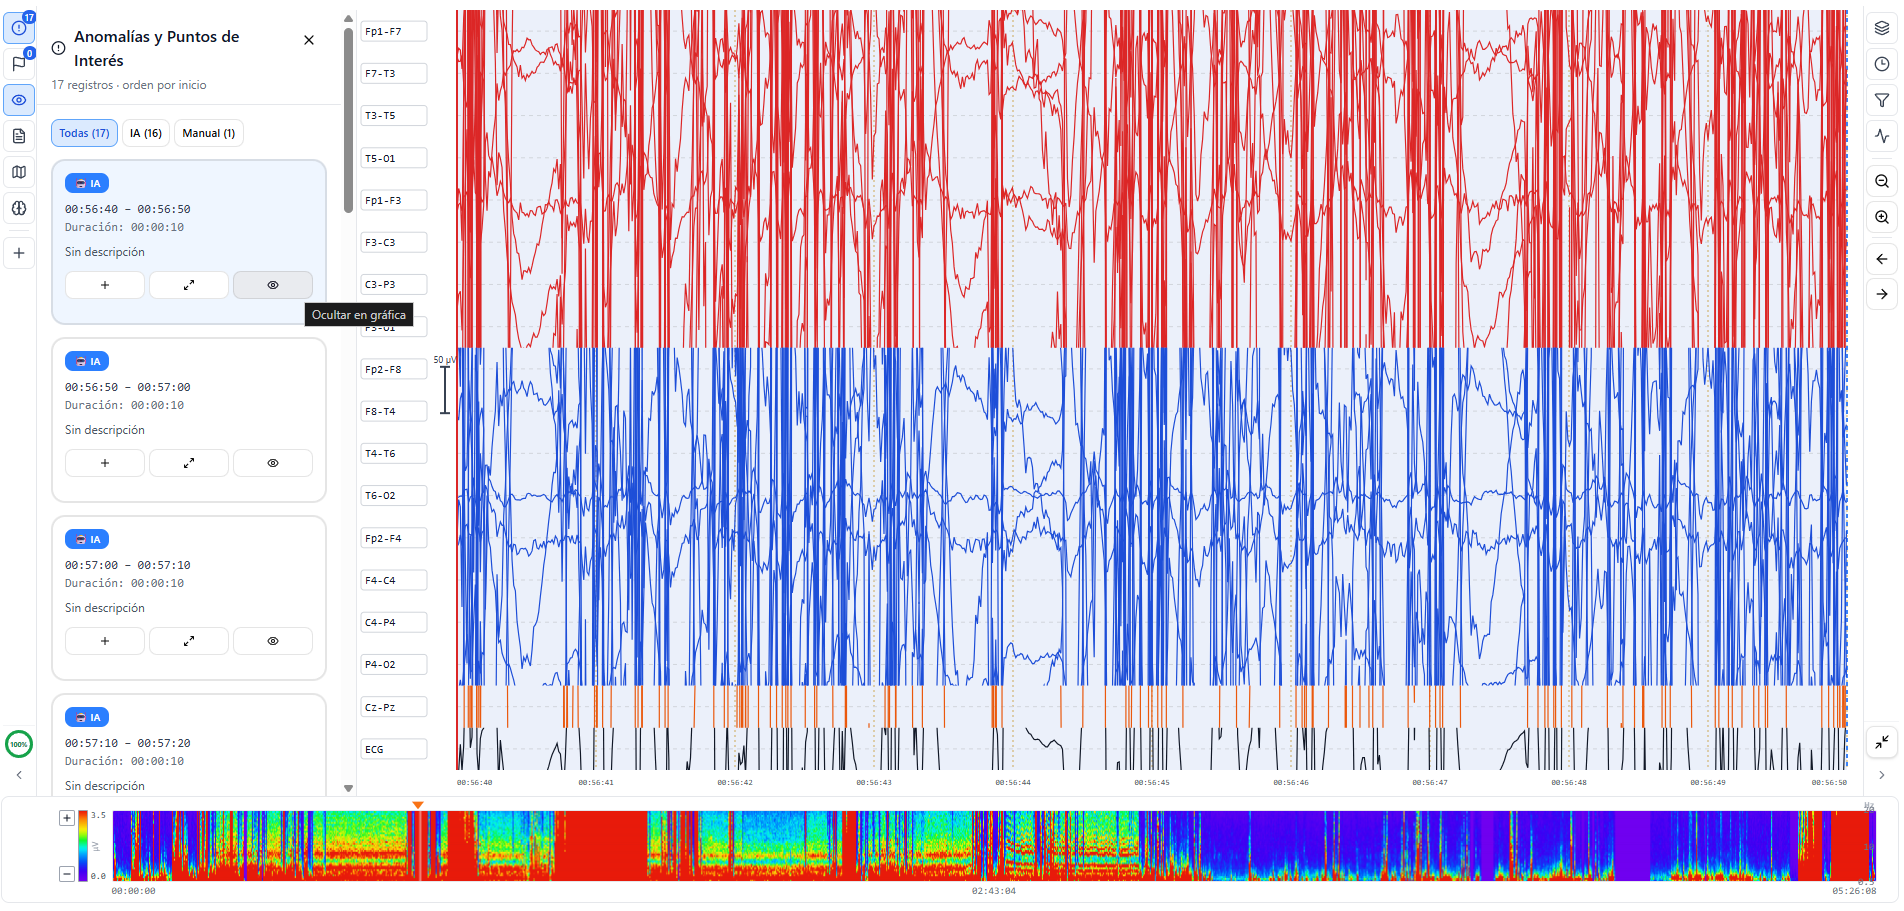
\includegraphics[width=0.85\textwidth]{Chapter6/Chapter6Figs/pf10_resultados_ia.png}
    \caption{Consulta de anomalías identificadas mediante inteligencia artificial en el visualizador EEG de EpilexIA.}
    \label{fig:pf10_resultados_ia}
\end{figure}

% Figura 6.16 - Detalle de anomalía
\begin{figure}[htbp]
    \centering
    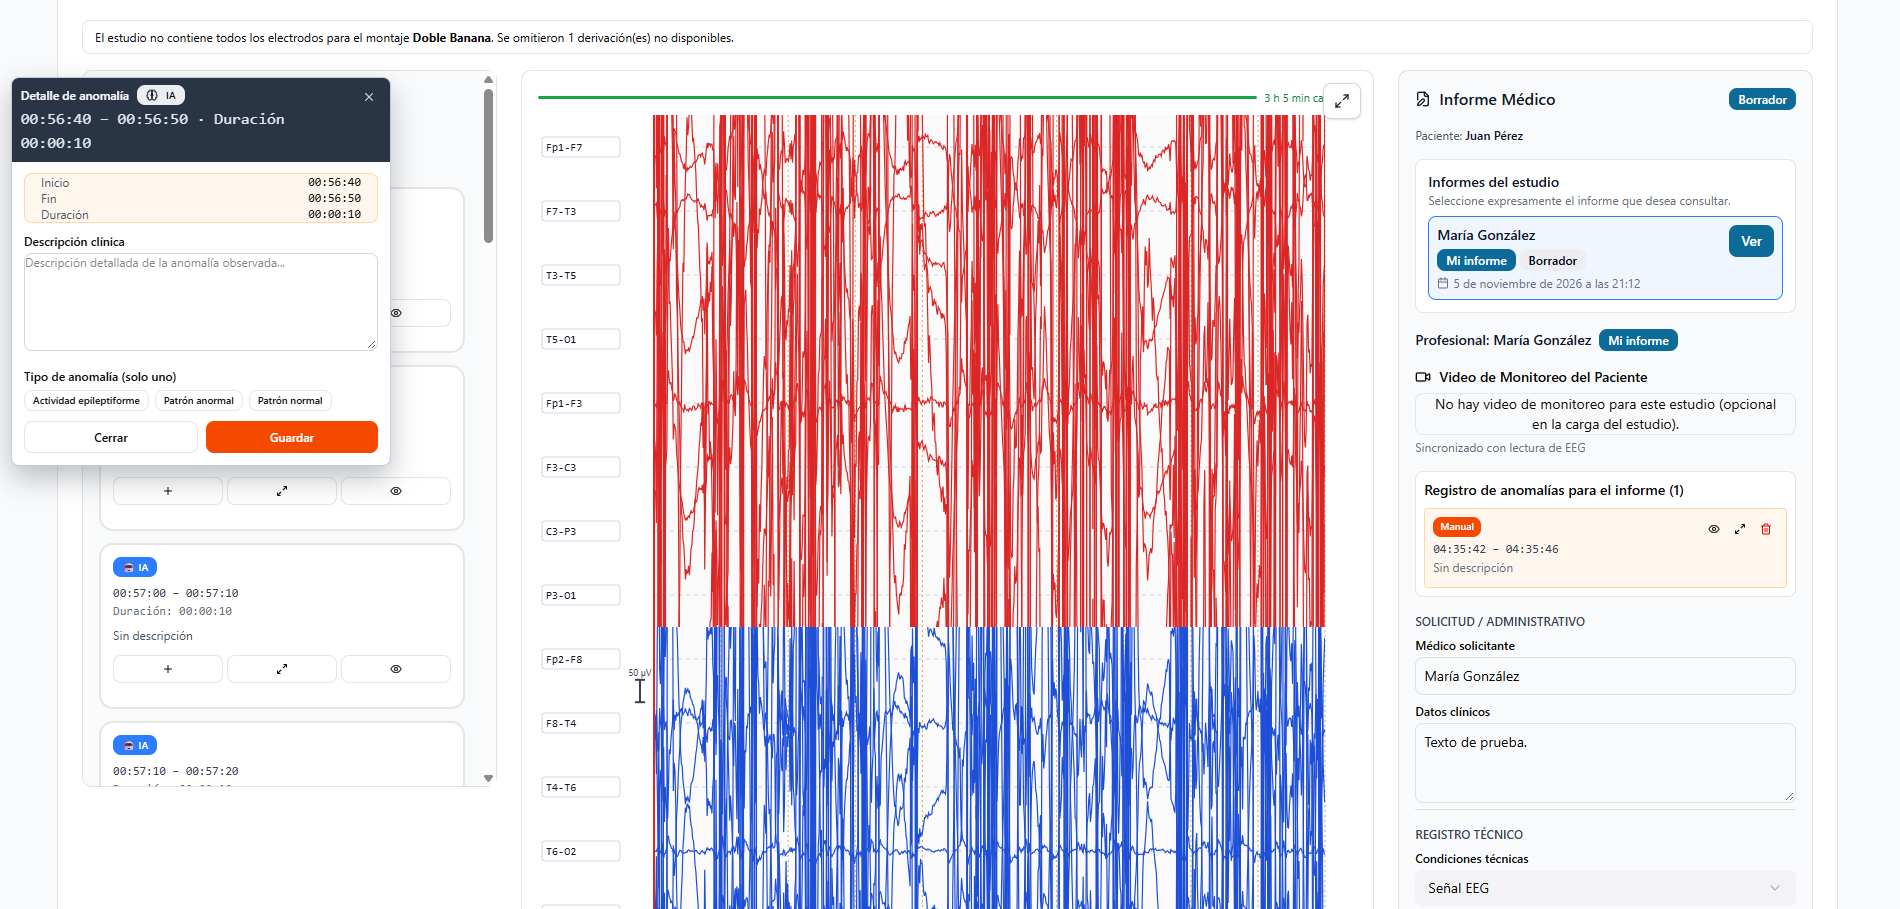
\includegraphics[width=0.85\textwidth]{Chapter6/Chapter6Figs/pf10_detalle_ia.png}
    \caption{Consulta del detalle y las referencias temporales de una anomalía identificada mediante inteligencia artificial en EpilexIA.}
    \label{fig:pf10_detalle_ia}
\end{figure}

% Figura 6.17 - Intervalo resaltado
\begin{figure}[htbp]
    \centering
    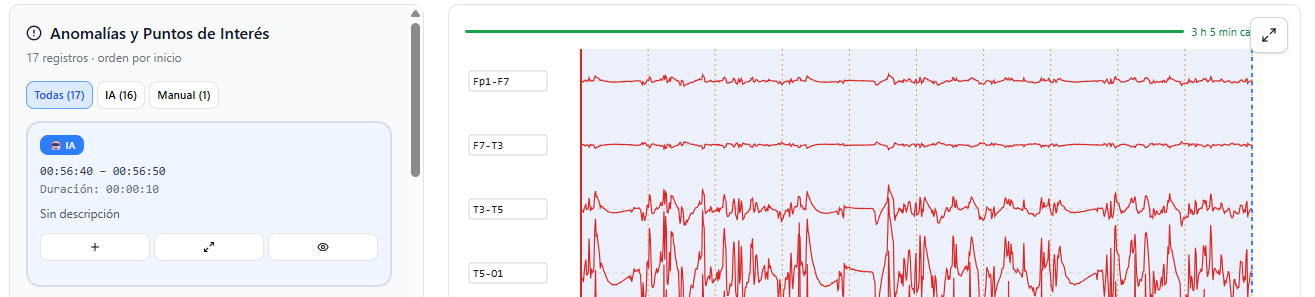
\includegraphics[width=0.85\textwidth]{Chapter6/Chapter6Figs/pf10_intervalo_ia.png}
    \caption{Resaltado del intervalo temporal correspondiente a una anomalía identificada mediante inteligencia artificial en EpilexIA.}
    \label{fig:pf10_intervalo_ia}
\end{figure}


\subsection{Resultados de la prueba de elaboración de informes médicos}

La prueba funcional PF-11 tuvo como objetivo verificar que EpilexIA permitiera elaborar y almacenar informes médicos asociados a estudios electroencefalográficos, así como consultar posteriormente la información registrada.

Para ejecutar la prueba, se accedió a un estudio EEG previamente registrado en la plataforma y se seleccionó el informe médico correspondiente al especialista autenticado. Se utilizó el informe identificado con el número 17, asociado al estudio 26, perteneciente a la profesional María González y en estado Borrador.

Durante la evaluación, se completaron diferentes campos del formulario utilizando información ficticia destinada exclusivamente a la comprobación funcional. Entre los campos evaluados se incluyeron los datos clínicos, las condiciones técnicas del registro, los ritmos de fondo durante vigilia y sueño, los hallazgos ictales e interictales, la conclusión breve y las observaciones. La Figura~\ref{fig:pf11_elaboracion_informe} presenta los campos completados durante la prueba.

Posteriormente, se guardó la información del informe médico y se cerró la sesión del usuario. A continuación, se inició una nueva sesión y se accedió nuevamente al informe asociado al estudio EEG.

Durante esta comprobación, se verificó que los valores previamente registrados permanecían disponibles, conservando su contenido en los diferentes apartados del informe. Asimismo, se observó que el sistema mantenía la identificación del estudio, el profesional responsable, el estado Borrador y la información de auditoría correspondiente a la creación y última actualización del registro.

La Figura~\ref{fig:pf11_persistencia_informe} presenta la consulta del informe médico después del nuevo inicio de sesión, mostrando la conservación de los datos clínicos y técnicos registrados.

Los resultados observados coincidieron con el comportamiento esperado para el caso PF-11, por lo que la prueba se clasificó como aprobada. La evaluación permitió verificar la elaboración de informes médicos, su asociación con un estudio EEG, el almacenamiento de los campos completados y la persistencia de la información después de una nueva sesión. La prueba se limitó a comprobar el comportamiento funcional de la plataforma, sin incluir una evaluación de la validez clínica del contenido registrado.


% Figura 6.18 - Elaboración del informe médico
\begin{figure}[htbp]
    \centering
    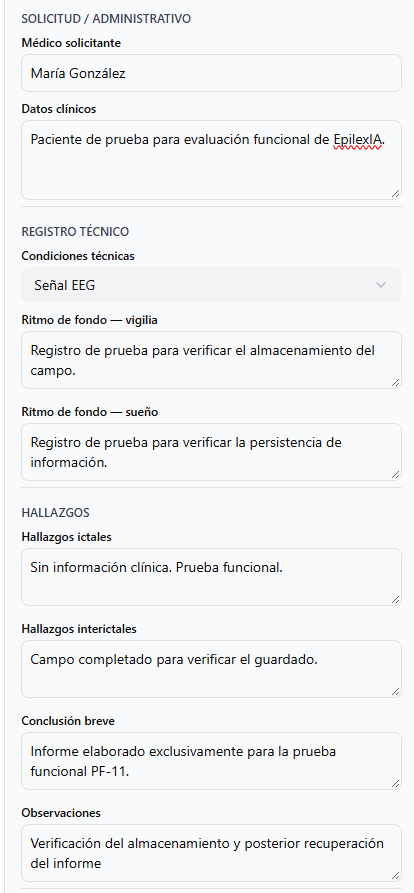
\includegraphics[width=0.65\textwidth]{Chapter6/Chapter6Figs/pf11_elaboracion_informe.png}
    \caption{Elaboración de un informe médico con información de prueba en EpilexIA.}
    \label{fig:pf11_elaboracion_informe}
\end{figure}

% Figura 6.19 - Persistencia del informe médico
\begin{figure}[htbp]
    \centering
    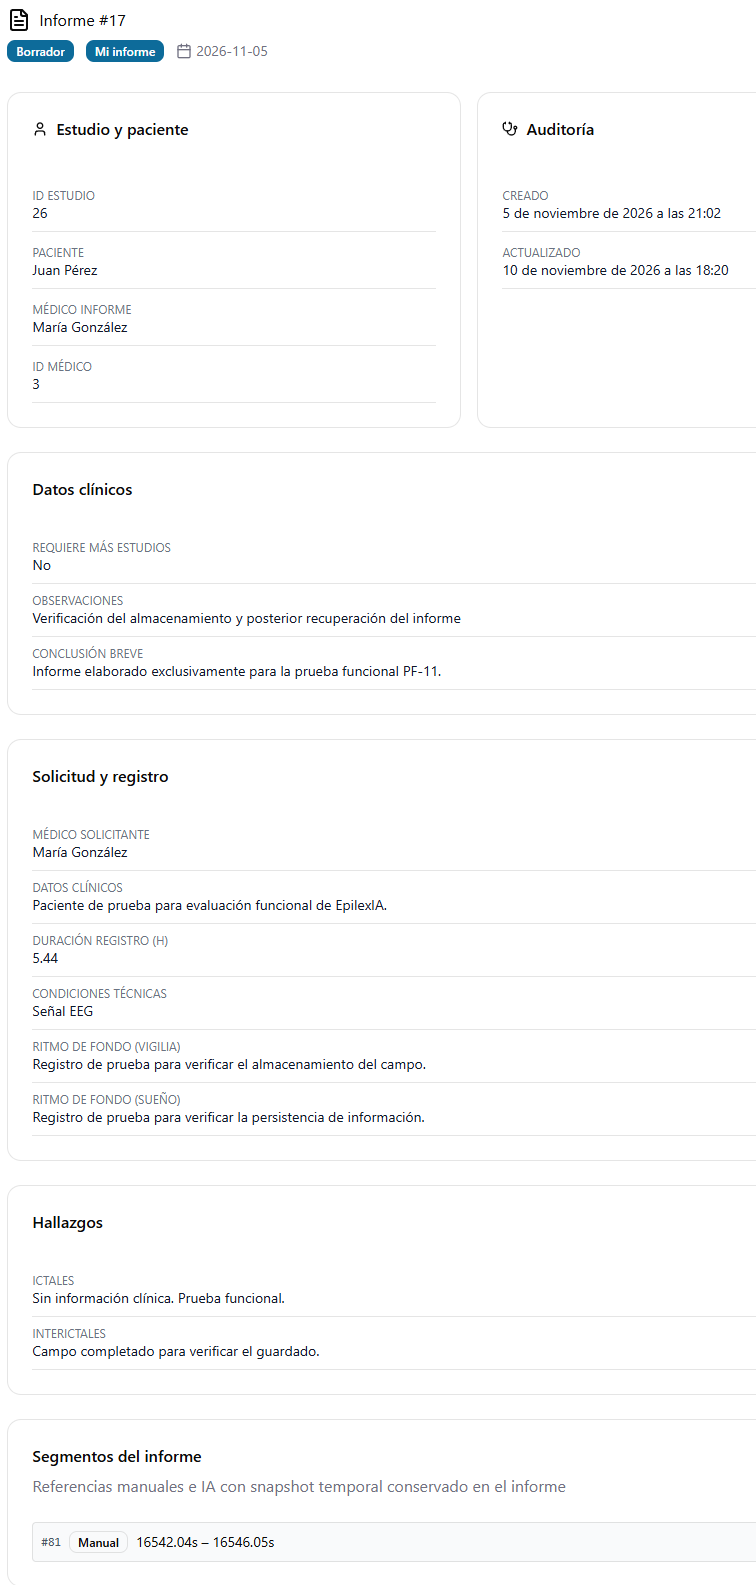
\includegraphics[width=0.70\textwidth]{Chapter6/Chapter6Figs/pf11_persistencia_informe.png}
    \caption{Consulta de un informe médico con conservación de los datos registrados después de iniciar una nueva sesión en EpilexIA.}
    \label{fig:pf11_persistencia_informe}
\end{figure}


\subsection{Resultados de la prueba de restricción de edición de informes médicos}

La prueba funcional PF-12 tuvo como objetivo verificar que EpilexIA restringiera la modificación de informes médicos pertenecientes a otros especialistas, permitiendo su consulta únicamente a los usuarios autorizados.

Para ejecutar la prueba, se utilizó el informe médico número 17, asociado al estudio EEG número 26, elaborado por la profesional María González y almacenado en estado Borrador. Se cerró la sesión de la profesional responsable y posteriormente se inició sesión con otro usuario que contaba con el perfil Especialista y acceso al estudio correspondiente.

Al ingresar al visualizador EEG y consultar el apartado de informes médicos, se comprobó que el sistema presentaba el informe de María González identificado mediante la etiqueta ``Solo lectura'', manteniendo visible su estado Borrador. Asimismo, se encontraba disponible la opción para crear un informe propio, diferenciando ambas operaciones. La Figura~\ref{fig:pf12_informe_solo_lectura} presenta esta configuración.

Posteriormente, se seleccionó la opción de consulta del informe perteneciente a María González. El sistema permitió visualizar los datos clínicos y técnicos previamente registrados, incluyendo las condiciones técnicas, los ritmos de fondo, los hallazgos y las observaciones.

Para comprobar la restricción de edición, se intentó introducir texto en los campos ``Datos clínicos'' y ``Conclusión breve''. En ambos casos, el sistema impidió modificar el contenido existente. La Figura~\ref{fig:pf12_campos_restringidos} muestra los campos del informe consultado en modo de solo lectura.

Los resultados observados coincidieron con el comportamiento esperado para el caso PF-12, por lo que la prueba funcional se clasificó como aprobada. La evaluación permitió verificar que un especialista autorizado podía consultar un informe médico ajeno sin modificar su contenido, incluso cuando este se encontraba en estado Borrador. La comprobación se limitó al comportamiento de la interfaz de usuario, sin incluir intentos de modificación mediante solicitudes directas a los servicios del \textit{backend}.


% Figura 6.20 - Informe médico ajeno en modo de solo lectura
\begin{figure}[htbp]
    \centering
    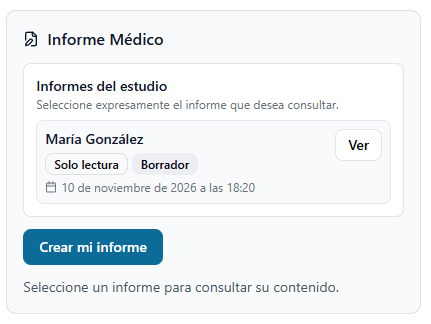
\includegraphics[width=0.75\textwidth]{Chapter6/Chapter6Figs/pf12_informe_solo_lectura.png}
    \caption{Identificación de un informe médico ajeno en modo de solo lectura en EpilexIA.}
    \label{fig:pf12_informe_solo_lectura}
\end{figure}

% Figura 6.21 - Campos del informe con edición restringida
\begin{figure}[htbp]
    \centering
    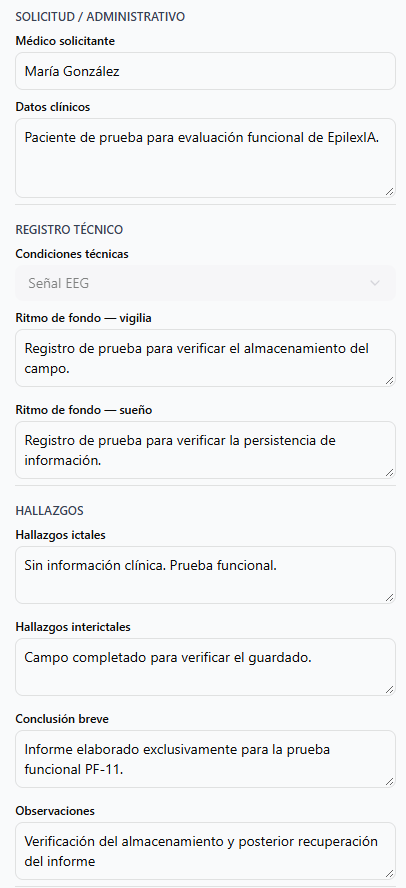
\includegraphics[width=0.65\textwidth]{Chapter6/Chapter6Figs/pf12_campos_restringidos.png}
    \caption{Consulta de los datos clínicos y técnicos de un informe médico ajeno con edición restringida en EpilexIA.}
    \label{fig:pf12_campos_restringidos}
\end{figure}

\FloatBarrier


\subsection{Resultados de la prueba de cierre de informes médicos}

La prueba funcional PF-13 tuvo como objetivo verificar que EpilexIA permitiera cerrar definitivamente un informe médico en estado Borrador, modificando su estado a Cerrado e impidiendo posteriores modificaciones de su contenido.

Para ejecutar la prueba, se utilizó el informe médico número 17, asociado al estudio EEG número 26 y perteneciente a la profesional María González. El informe se encontraba inicialmente en estado Borrador y contenía información de prueba previamente registrada durante la evaluación funcional PF-11.

En primer lugar, se accedió al informe médico y se seleccionó la opción \textit{Cerrar informe}. El sistema presentó una ventana de confirmación en la que se advertía que el cierre sería definitivo, afectaría únicamente al informe seleccionado y no permitiría modificaciones posteriores. La Figura~\ref{fig:pf13_confirmacion_cierre} presenta esta ventana de confirmación.

Posteriormente, se confirmó la operación de cierre. Al consultar nuevamente el formulario, se comprobó que los campos del informe ya no permitían modificaciones y que la opción \textit{Guardar informe} se encontraba deshabilitada. La Figura~\ref{fig:pf13_edicion_restringida} muestra el comportamiento observado después del cierre.

Adicionalmente, se realizó una comprobación de persistencia. Para ello, se cerró la sesión del usuario y posteriormente se volvió a acceder a la plataforma. Al consultar nuevamente el estudio EEG, se verificó que el informe conservaba el estado Cerrado y se encontraba identificado como de solo lectura.

Durante esta comprobación, también se observó que el sistema impedía crear nuevos informes médicos asociados al mismo estudio, mostrando un mensaje que indicaba la existencia de un informe previamente cerrado. La Figura~\ref{fig:pf13_persistencia_cierre} presenta el estado del informe después de iniciar una nueva sesión.

Los resultados observados coincidieron con el comportamiento esperado para el caso PF-13, por lo que la prueba funcional se clasificó como aprobada. La evaluación permitió verificar el cierre definitivo de un informe médico, la restricción de edición desde la interfaz, la conservación del estado Cerrado después de una nueva sesión y la restricción de creación de nuevos informes en el estudio correspondiente. La prueba se limitó a comprobar el comportamiento funcional de la plataforma, sin incluir intentos de modificación mediante solicitudes directas a los servicios del \textit{backend}.


% Figura 6.22 - Confirmación del cierre
\begin{figure}[htbp]
    \centering
    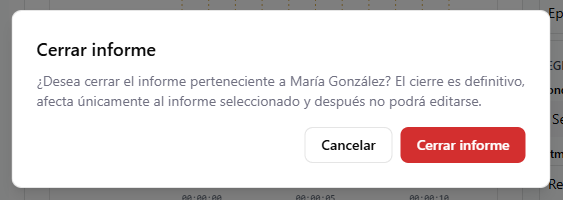
\includegraphics[width=0.75\textwidth]{Chapter6/Chapter6Figs/pf13_confirmacion_cierre.png}
    \caption{Confirmación del cierre definitivo de un informe médico en EpilexIA.}
    \label{fig:pf13_confirmacion_cierre}
\end{figure}

% Figura 6.23 - Restricción de edición
\begin{figure}[htbp]
    \centering
    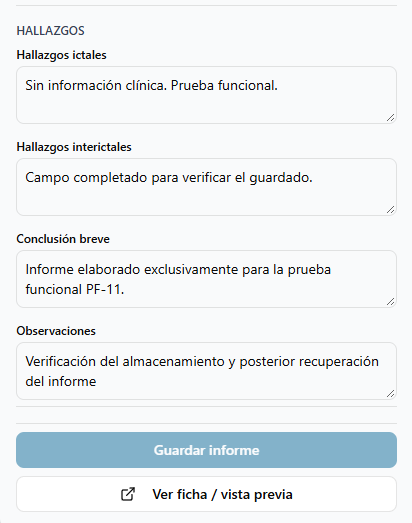
\includegraphics[width=0.65\textwidth]{Chapter6/Chapter6Figs/pf13_edicion_restringida.png}
    \caption{Restricción de edición y guardado de un informe médico después de su cierre en EpilexIA.}
    \label{fig:pf13_edicion_restringida}
\end{figure}

% Figura 6.24 - Persistencia del cierre
\begin{figure}[htbp]
    \centering
    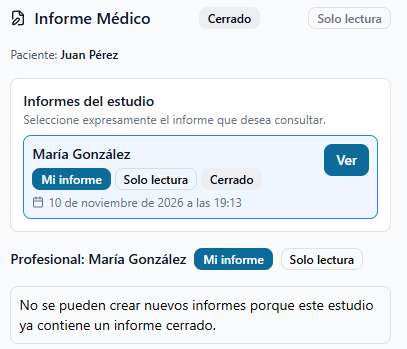
\includegraphics[width=0.70\textwidth]{Chapter6/Chapter6Figs/pf13_persistencia_cierre.png}
    \caption{Persistencia del estado Cerrado y restricción de creación de nuevos informes después de iniciar una nueva sesión en EpilexIA.}
    \label{fig:pf13_persistencia_cierre}
\end{figure}
\FloatBarrier


\subsection{Resultados de la prueba de control de acceso según roles}

La prueba funcional PF-14 tuvo como objetivo verificar que EpilexIA presentara las funcionalidades correspondientes al rol del usuario autenticado y restringiera el acceso a determinados módulos para los perfiles que no contaran con los permisos necesarios.

Para ejecutar la prueba, se utilizaron tres cuentas de usuario con los perfiles Administrador, Técnico y Especialista. Se inició sesión de manera independiente con cada cuenta y se examinó el panel de control, prestando especial atención a las opciones disponibles en el apartado de accesos rápidos.

En primer lugar, se inició sesión con una cuenta de Administrador. Se comprobó que el sistema presentaba las opciones de Gestión de Usuarios, Estudios EEG y Reportes, además de los indicadores generales y el apartado de actividad reciente. La Figura~\ref{fig:pf14_rol_administrador} muestra el panel correspondiente a este perfil.

Posteriormente, se inició sesión con el usuario Carlos Fernández, correspondiente al perfil Técnico. Durante la evaluación, se observó que el panel únicamente presentaba el acceso rápido a Estudios EEG, sin mostrar las opciones de Gestión de Usuarios ni Reportes. No obstante, permanecían visibles los indicadores generales y la actividad reciente del sistema, como se observa en la Figura~\ref{fig:pf14_rol_tecnico}.

A continuación, se inició sesión con la profesional María González, correspondiente al perfil Especialista. Se comprobó que el sistema presentaba los accesos rápidos a Estudios EEG y Reportes, mientras que la opción de Gestión de Usuarios no se encontraba disponible. La Figura~\ref{fig:pf14_rol_especialista} muestra la configuración del panel correspondiente a este perfil.

Adicionalmente, se realizaron comprobaciones de acceso directo a rutas restringidas. Con las sesiones de los usuarios Técnico y Especialista, se intentó acceder manualmente a la ruta \texttt{/app/users}, correspondiente al módulo de Gestión de Usuarios. En ambos casos, el sistema impidió la navegación hacia dicho módulo y redirigió automáticamente al usuario a la ruta \texttt{/app/dashboard}.

Los resultados observados coincidieron con el comportamiento esperado para el caso PF-14, por lo que la prueba funcional se clasificó como aprobada. La evaluación permitió verificar la diferenciación de los accesos visibles según el rol autenticado y la restricción de navegación directa hacia el módulo de Gestión de Usuarios para los perfiles Técnico y Especialista. La comprobación se limitó al comportamiento de la interfaz y sus mecanismos de navegación, sin incluir solicitudes directas a los servicios del \textit{backend}.


% Figura 6.25 - Rol Administrador
\begin{figure}[htbp]
    \centering
    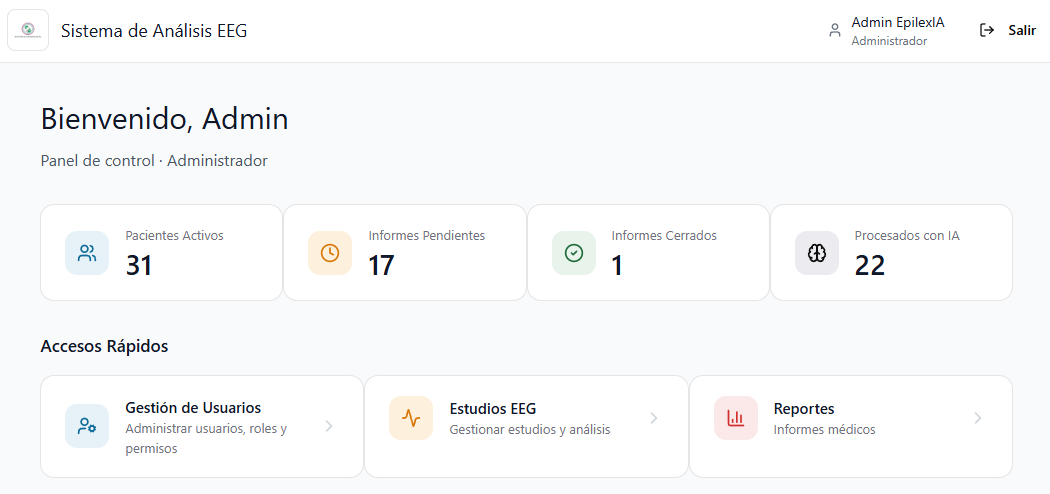
\includegraphics[width=\textwidth]{Chapter6/Chapter6Figs/pf14_rol_administrador.png}
    \caption{Panel de control del Administrador con acceso a Gestión de Usuarios, Estudios EEG y Reportes en EpilexIA.}
    \label{fig:pf14_rol_administrador}
\end{figure}

% Figura 6.26 - Rol Técnico
\begin{figure}[htbp]
    \centering
    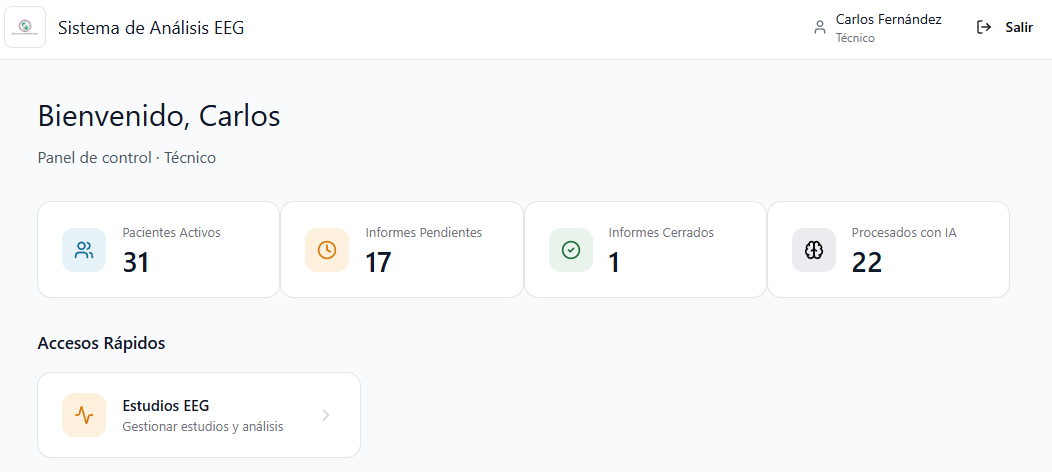
\includegraphics[width=\textwidth]{Chapter6/Chapter6Figs/pf14_rol_tecnico.png}
    \caption{Panel de control del Técnico con acceso rápido a Estudios EEG y restricciones de acceso a otros módulos en EpilexIA.}
    \label{fig:pf14_rol_tecnico}
\end{figure}

% Figura 6.27 - Rol Especialista
\begin{figure}[htbp]
    \centering
    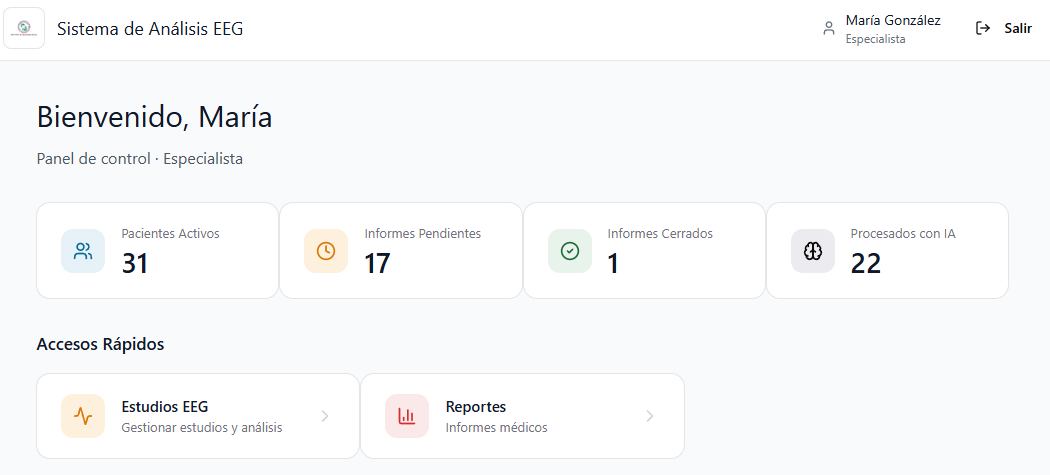
\includegraphics[width=\textwidth]{Chapter6/Chapter6Figs/pf14_rol_especialista.png}
    \caption{Panel de control del Especialista con acceso a Estudios EEG y Reportes, sin acceso a Gestión de Usuarios en EpilexIA.}
    \label{fig:pf14_rol_especialista}
\end{figure}

\FloatBarrier


\subsection{Resultados de la prueba de consulta de auditoría}

La prueba funcional PF-15 tuvo como objetivo verificar que EpilexIA permitiera consultar los registros de auditoría generados durante la utilización de la plataforma, de acuerdo con los permisos establecidos para los usuarios autenticados.

Para ejecutar la prueba, se inició sesión con una cuenta de Administrador y se accedió al módulo de auditoría mediante la opción \textit{Ver todas las auditorías}, disponible en el panel de control. Se comprobó que el sistema presentaba un historial de operaciones con información sobre la fecha y hora, el tipo de evento, el actor responsable, su rol y el contexto asociado a cada registro.

Entre las operaciones identificadas se encontraban la creación y actualización de informes médicos, el cierre de informes, la creación de estudios EEG y las ejecuciones de análisis mediante inteligencia artificial. Asimismo, se observaron registros correspondientes a las pruebas funcionales realizadas anteriormente, incluyendo el cierre del informe médico número 17, asociado al estudio EEG número 26. La Figura~\ref{fig:pf15_historial_auditoria} presenta la consulta general del historial de auditoría.

Posteriormente, se evaluaron los mecanismos de filtrado disponibles en el módulo. En primer lugar, se seleccionó la fecha 10/11/2026 y se comprobó que el sistema presentaba únicamente dos registros correspondientes a ese día: la actualización y el cierre de un informe médico. La Figura~\ref{fig:pf15_filtro_fecha} muestra los resultados obtenidos mediante este criterio.

A continuación, se utilizó el filtro por evento, introduciendo el texto \textit{Informe cerrado}. Como resultado, el sistema presentó un único registro correspondiente al cierre del informe médico número 17, realizado por la profesional María González. La Figura~\ref{fig:pf15_filtro_evento} muestra esta consulta.

Adicionalmente, se comprobaron los filtros por actor y rol. Al introducir el nombre María en el campo correspondiente al actor, se visualizaron operaciones asociadas a la profesional María González. Posteriormente, al seleccionar el rol Especialista, manteniendo el filtro por actor, los registros presentados correspondían a los criterios establecidos.

Finalmente, se realizaron comprobaciones de acceso utilizando cuentas correspondientes a los perfiles Técnico y Especialista. En ambos casos, el sistema permitió acceder al módulo de auditoría y consultar registros generados por diferentes usuarios y procesos. En la versión evaluada, la consulta de auditoría está disponible para los tres perfiles, de modo que técnicos y especialistas pueden conocer las acciones realizadas por otros usuarios, como mecanismo de control cruzado. Los registros describen acciones, con su tipo, actor, rol, fecha e identificadores de contexto, y no incluyen el contenido clínico de las anomalías ni de los informes. Esta consulta es independiente del módulo de informes médicos, cuyo acceso se restringe según el perfil (PF-14). La Figura~\ref{fig:pf15_auditoria_tecnico} presenta la consulta realizada desde una cuenta con perfil Técnico.

Los resultados observados coincidieron con el comportamiento esperado para el caso PF-15, por lo que la prueba funcional se clasificó como aprobada. La evaluación permitió verificar la disponibilidad del historial de auditoría, la identificación de las operaciones registradas, el funcionamiento de los filtros de consulta y el acceso al módulo desde los tres roles definidos en EpilexIA. La prueba se limitó a comprobar el comportamiento funcional de la interfaz, sin incluir una evaluación de la integridad de los registros almacenados ni pruebas directas de autorización sobre los servicios del \textit{backend}.


% Figura 6.28 - Historial general de auditoría
\begin{figure}[htbp]
    \centering
    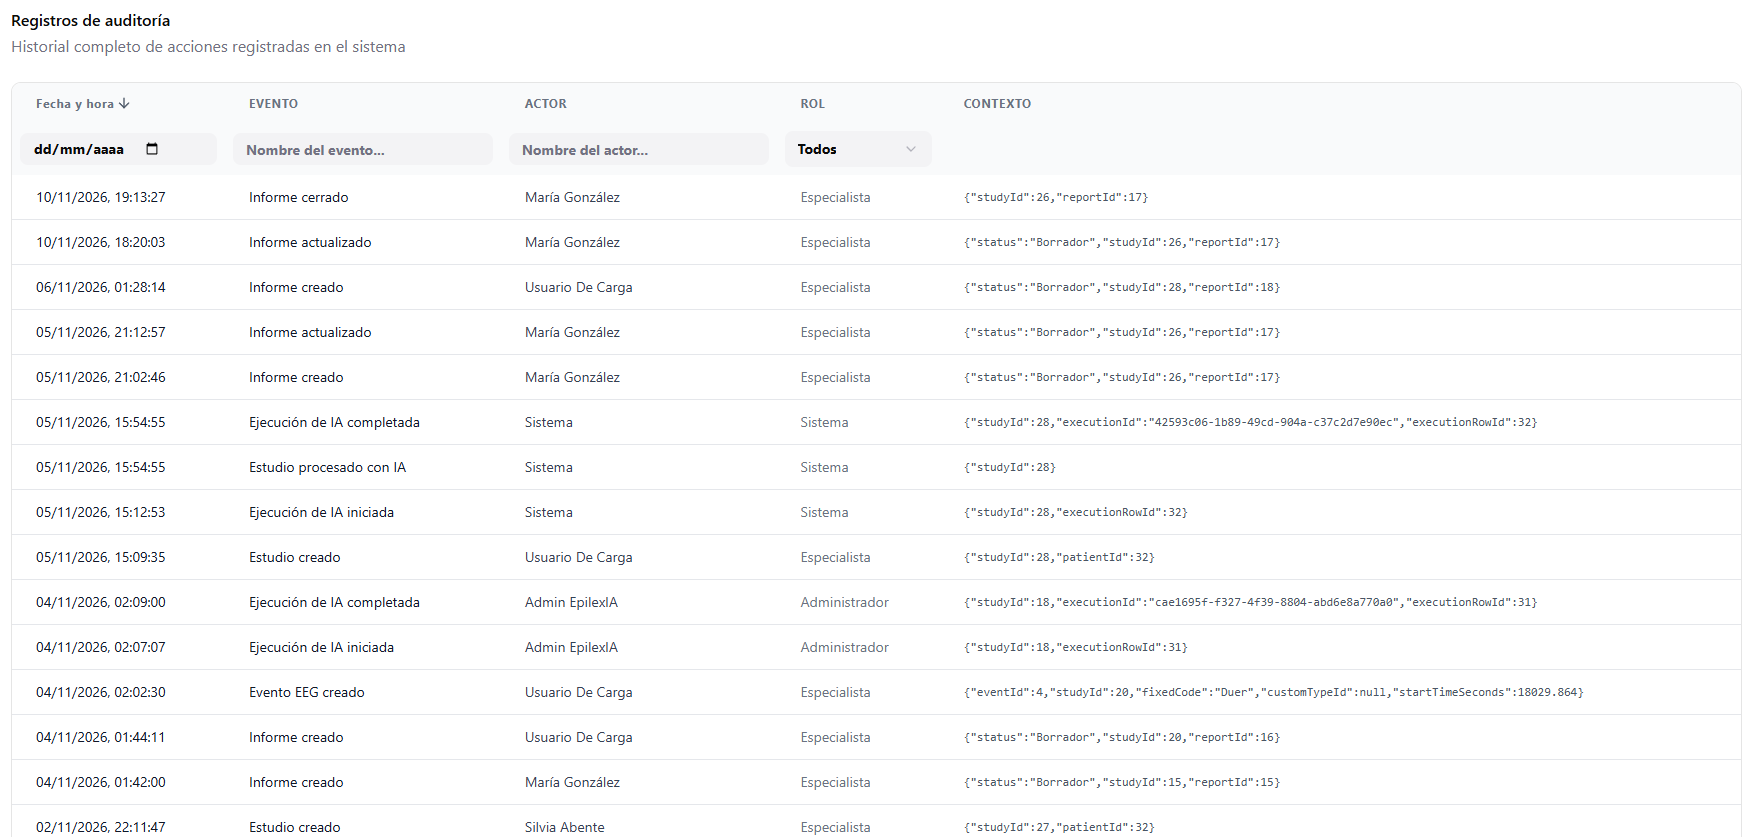
\includegraphics[width=0.95\textwidth]{Chapter6/Chapter6Figs/pf15_historial_auditoria.png}
    \caption{Consulta del historial de auditoría con identificación de eventos, actores, roles y contexto de las operaciones en EpilexIA.}
    \label{fig:pf15_historial_auditoria}
\end{figure}

% Figura 6.29 - Filtro por fecha
\begin{figure}[htbp]
    \centering
    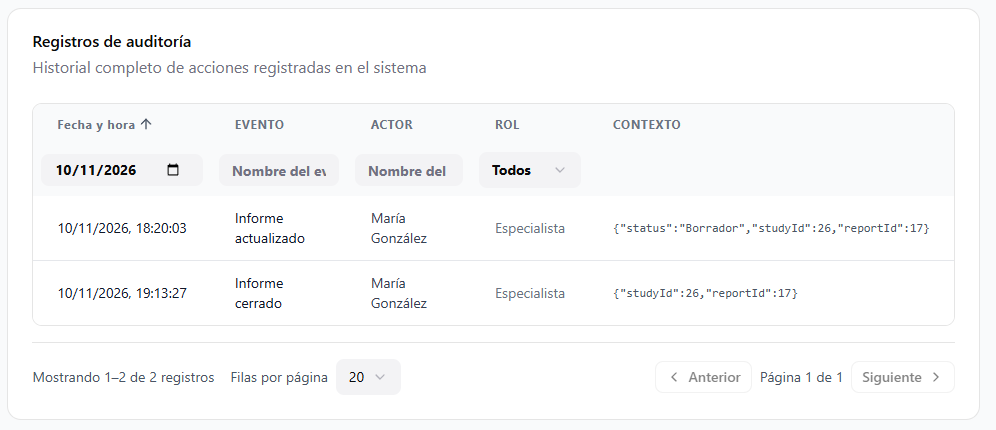
\includegraphics[width=0.95\textwidth]{Chapter6/Chapter6Figs/pf15_filtro_fecha.png}
    \caption{Consulta de registros de auditoría correspondientes al 10 de noviembre de 2026 en EpilexIA.}
    \label{fig:pf15_filtro_fecha}
\end{figure}

% Figura 6.30 - Filtro por evento
\begin{figure}[htbp]
    \centering
    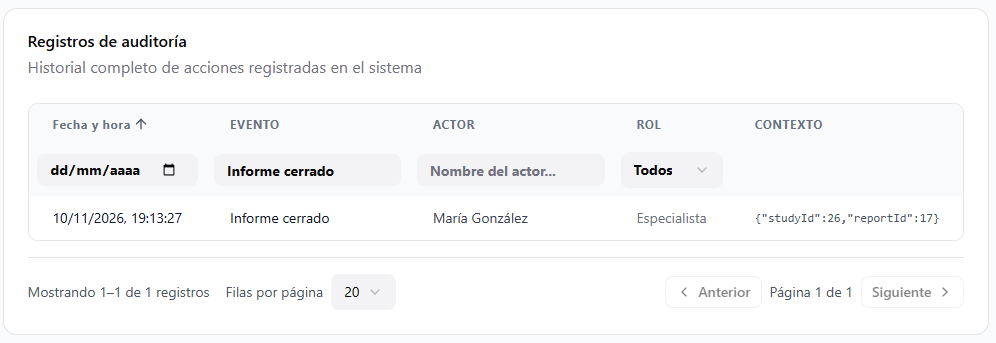
\includegraphics[width=0.95\textwidth]{Chapter6/Chapter6Figs/pf15_filtro_evento.png}
    \caption{Consulta de registros de auditoría mediante el filtro por evento de cierre de informe médico en EpilexIA.}
    \label{fig:pf15_filtro_evento}
\end{figure}

% Figura 6.31 - Auditoría con perfil Técnico
\begin{figure}[htbp]
    \centering
    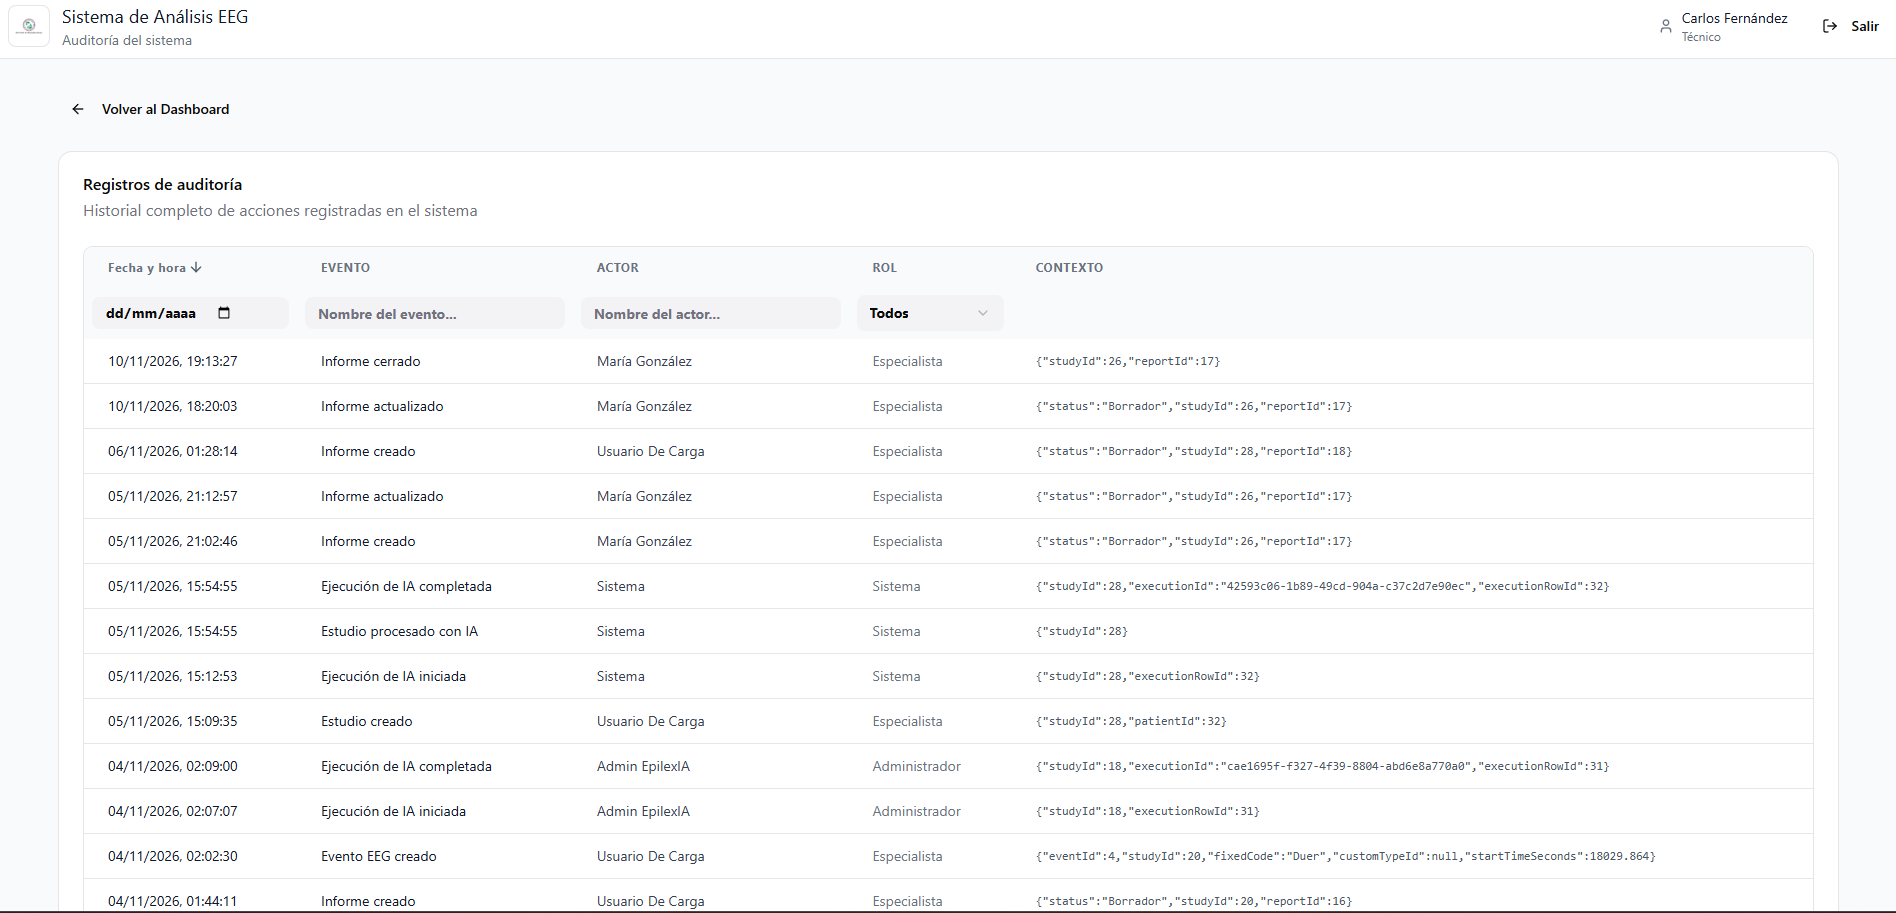
\includegraphics[width=0.95\textwidth]{Chapter6/Chapter6Figs/pf15_auditoria_tecnico.png}
    \caption{Consulta del historial de auditoría desde una cuenta con perfil Técnico en EpilexIA.}
    \label{fig:pf15_auditoria_tecnico}
\end{figure}

\FloatBarrier


\subsection{Síntesis de los resultados de las pruebas funcionales}
\label{subsec:sintesis_pruebas_funcionales}

Las pruebas funcionales realizadas permitieron evaluar el comportamiento de EpilexIA frente a los escenarios definidos para las principales funcionalidades de la plataforma. La evaluación comprendió quince casos de prueba, identificados desde PF-01 hasta PF-15, cuyos procedimientos y resultados fueron documentados en los apartados anteriores.

Los casos evaluados abarcaron la autenticación y validación de credenciales, el registro de pacientes y estudios EEG, la carga y visualización de señales electroencefalográficas, la configuración de montajes y filtros, el registro manual de anomalías, la consulta de resultados de inteligencia artificial, la elaboración y cierre de informes médicos, el control de acceso según roles y la consulta de registros de auditoría.

El Cuadro~\ref{tab:sintesis_pruebas_funcionales} presenta una síntesis de los casos evaluados y sus respectivos resultados.

\begin{longtable}{|p{1.5cm}|p{8cm}|p{2.5cm}|}
\caption{Síntesis de los resultados de las pruebas funcionales de EpilexIA.}
\label{tab:sintesis_pruebas_funcionales}\\
\hline
\textbf{ID} & \textbf{Funcionalidad evaluada} & \textbf{Resultado} \\
\hline
\endfirsthead

\multicolumn{3}{c}{\textit{Continuación del Cuadro \thetable}}\\
\hline
\textbf{ID} & \textbf{Funcionalidad evaluada} & \textbf{Resultado} \\
\hline
\endhead

PF-01 & Autenticación de usuarios & Aprobada \\ \hline
PF-02 & Validación de credenciales & Aprobada \\ \hline
PF-03 & Registro de pacientes & Aprobada \\ \hline
PF-04 & Registro de estudios EEG & Aprobada \\ \hline
PF-05 & Carga de archivos EEG & Aprobada \\ \hline
PF-06 & Visualización de señales EEG & Aprobada \\ \hline
PF-07 & Configuración de montajes & Aprobada \\ \hline
PF-08 & Configuración de filtros & Aprobada \\ \hline
PF-09 & Registro manual de anomalías & Aprobada \\ \hline
PF-10 & Consulta de resultados de IA & Aprobada \\ \hline
PF-11 & Elaboración de informes médicos & Aprobada \\ \hline
PF-12 & Restricción de edición de informes & Aprobada \\ \hline
PF-13 & Cierre de informes médicos & Aprobada \\ \hline
PF-14 & Control de acceso por roles & Aprobada \\ \hline
PF-15 & Consulta de auditoría & Aprobada \\ \hline

\end{longtable}


En los casos documentados como aprobados, los resultados observados coincidieron con los comportamientos esperados establecidos para los escenarios de evaluación. Las comprobaciones permitieron examinar las operaciones principales de la plataforma y su funcionamiento desde la perspectiva de los usuarios.

En relación con la gestión de la información, se evaluaron los mecanismos de autenticación, el registro de pacientes y la creación de estudios EEG. Asimismo, se examinó la capacidad del sistema para cargar archivos de señales electroencefalográficas y presentar su contenido mediante el visualizador.

Respecto de las herramientas de análisis, se realizaron comprobaciones sobre la configuración de montajes y filtros, el registro manual de anomalías y la consulta de resultados generados mediante inteligencia artificial. Estas pruebas se orientaron a verificar la disponibilidad y el funcionamiento de las operaciones implementadas, sin evaluar la precisión diagnóstica de los modelos utilizados.

Por otra parte, las pruebas relacionadas con los informes médicos permitieron comprobar su elaboración, almacenamiento y consulta posterior. También se verificaron las restricciones de edición sobre informes pertenecientes a otros especialistas y el comportamiento de los informes después de su cierre definitivo.

En cuanto al control de acceso, se observaron diferencias en las funcionalidades disponibles para los perfiles Administrador, Técnico y Especialista. Adicionalmente, se comprobó la disponibilidad del historial de auditoría y el funcionamiento de los mecanismos de consulta y filtrado de los registros.

En conjunto, los resultados proporcionan evidencia del funcionamiento de las principales características de EpilexIA dentro de los escenarios evaluados. No obstante, las conclusiones se limitan al alcance de las pruebas funcionales ejecutadas y no constituyen una validación integral de la seguridad, el rendimiento, la integridad de los datos ni la precisión clínica del sistema.


\section{Pruebas de integración}
\label{sec:pruebas_integracion}

% Introducción general resumida.

Las pruebas de integración tienen como propósito verificar la comunicación y el intercambio de información entre los componentes que conforman la arquitectura de EpilexIA. A diferencia de las pruebas funcionales, orientadas a comprobar el comportamiento de operaciones específicas desde la perspectiva del usuario, estas pruebas se centran en las interacciones entre los distintos servicios de la plataforma.

La evaluación comprende los mecanismos de comunicación, persistencia y coordinación entre los componentes del sistema, incluyendo la interfaz web, el \textit{backend} clínico, las bases de datos y los servicios encargados del procesamiento mediante inteligencia artificial.

En los siguientes apartados se describen el objetivo y alcance de la evaluación, los mecanismos de comunicación identificados y los casos de prueba definidos para verificar las integraciones implementadas.


\subsection{Objetivo y alcance de las pruebas de integración}

\label{subsec:objetivo_pruebas_integracion}

El objetivo de las pruebas de integración es comprobar que los componentes de EpilexIA intercambian información de manera consistente y permiten completar las operaciones que requieren la participación de varios servicios. Para ello, se consideran tanto las solicitudes realizadas desde la interfaz web como las operaciones internas de persistencia, coordinación y consulta de resultados.

El alcance de la evaluación comprende la autenticación y la gestión de sesiones, la comunicación entre la interfaz web y el \textit{backend} clínico, el almacenamiento y la recuperación de información clínica, así como la asociación entre los archivos EEG y sus respectivos registros en la base de datos. También se incluyen las interacciones necesarias para iniciar y supervisar los procesos de análisis mediante inteligencia artificial.

En relación con el procesamiento asíncrono, se contempla la verificación del registro de solicitudes, la recuperación de trabajos pendientes por parte del motor de inteligencia artificial, la actualización de sus estados y la disponibilidad de los resultados para su consulta desde la plataforma. Asimismo, se consideran los mecanismos de auditoría y el tratamiento de determinadas condiciones de error durante la comunicación entre servicios.


La ejecución de las pruebas de integración se llevó a cabo mediante operaciones controladas sobre la plataforma, la observación de solicitudes y respuestas HTTP, la revisión de registros de ejecución y consultas de solo lectura a las bases de datos, según las evidencias disponibles para cada caso. Estos procedimientos permitieron contrastar el comportamiento observado con los resultados esperados y determinar el grado de verificación alcanzado en las integraciones evaluadas.


La evaluación se limita a los mecanismos de interoperabilidad, persistencia y coordinación entre componentes. Por tanto, no pretende determinar la precisión diagnóstica de los modelos de inteligencia artificial ni medir el rendimiento computacional del procesamiento EEG. Estos aspectos se abordan de manera diferenciada en las secciones correspondientes del presente capítulo.


\subsection{Componentes y mecanismos de comunicación}

\label{subsec:componentes_integracion}

La arquitectura de EpilexIA está organizada en componentes que interactúan mediante servicios HTTP, conexiones a bases de datos y volúmenes de almacenamiento compartidos. Esta organización permite separar las responsabilidades de presentación, gestión de información clínica y procesamiento de señales electroencefalográficas.


La interfaz web está desarrollada con React y TypeScript. En el entorno de despliegue mediante contenedores, los archivos estáticos son servidos por Nginx, que también actúa como intermediario para las solicitudes dirigidas al \textit{backend} clínico. La comunicación con Spring Boot se realiza mediante solicitudes HTTP y respuestas en formato JSON. Para las operaciones protegidas, el cliente incorpora un \textit{token} de autenticación JWT, que permite identificar al usuario y verificar sus permisos.


El \textit{backend} clínico está implementado con Spring Boot y desplegado sobre WildFly. Este componente concentra las reglas de negocio, los mecanismos de autorización y las operaciones relacionadas con pacientes, estudios EEG, informes médicos y auditoría. La persistencia se realiza mediante Spring Data JPA e Hibernate, utilizando una base de datos PostgreSQL cuyo esquema principal se denomina \texttt{epilexia}.

Los archivos de señales EEG se almacenan físicamente en un volumen compartido, mientras que sus rutas y metadatos se registran en la base de datos principal. De esta manera, los componentes que participan en el procesamiento pueden acceder a los archivos sin necesidad de transferir su contenido completo mediante solicitudes HTTP.

Para las operaciones relacionadas con inteligencia artificial, Spring Boot establece una comunicación HTTP directa con un servicio desarrollado mediante FastAPI. Esta comunicación permite solicitar ejecuciones de análisis, consultar sus estados, recuperar las anomalías detectadas y solicitar la generación de espectrogramas. También contempla el intercambio de información correspondiente a anotaciones manuales y ventanas de análisis confirmadas en los informes médicos.

Mediante el mecanismo denominado \texttt{pgqueue}, FastAPI utiliza una segunda base de datos PostgreSQL para registrar y coordinar los trabajos de procesamiento. Las solicitudes se almacenan en una cola persistente, representada principalmente por la tabla \texttt{ai\_executions}. El motor de inteligencia artificial consulta los trabajos pendientes, ejecuta el procesamiento de las señales EEG y registra los estados y resultados obtenidos.

La coordinación entre FastAPI y el motor se realiza mediante esta base de datos compartida, sin establecer una comunicación HTTP directa entre ambos componentes. Los resultados del análisis se almacenan principalmente en la tabla \texttt{ai\_results}, desde donde pueden ser recuperados posteriormente por el servicio FastAPI.

Durante el procesamiento, Spring Boot mantiene una referencia local de cada ejecución y consulta su estado mediante FastAPI. Por su parte, la interfaz web realiza consultas periódicas al \textit{backend} clínico para actualizar la información presentada al usuario. Este mecanismo permite supervisar el avance de las ejecuciones asíncronas y consultar los resultados una vez finalizado el análisis.

En conjunto, estos mecanismos permiten identificar las principales interfaces de integración de EpilexIA y establecer los casos de prueba necesarios para verificar la comunicación, la persistencia de información y la coordinación entre los componentes del sistema.


\subsection{Definición de los casos de prueba de integración}
\label{subsec:casos_pruebas_integracion}

A partir de los mecanismos de comunicación identificados en la arquitectura de EpilexIA, se definieron diecisiete casos de prueba de integración, orientados a verificar el intercambio de información y la coordinación entre los distintos componentes de la plataforma.

Los casos contemplan la autenticación y la gestión de sesiones, la persistencia de información clínica, la asociación entre los estudios EEG y sus archivos, la comunicación con el servicio de inteligencia artificial, la coordinación del procesamiento asíncrono, la recuperación de resultados y el registro de eventos de auditoría.

Asimismo, se incluyen situaciones destinadas a evaluar el comportamiento de las interfaces ante determinadas condiciones de error, como la indisponibilidad temporal del servicio de inteligencia artificial o la saturación de la cola de procesamiento. Estas situaciones se ejecutaron en un entorno de pruebas local, que replica el despliegue mediante los mismos contenedores, para evitar interferencias con la instancia utilizada en el hospital.

En el Cuadro~\ref{tab:casos_pruebas_integracion} se presentan los casos definidos, los componentes involucrados y los resultados esperados. Posteriormente, se describen las pruebas ejecutadas y las evidencias obtenidas.


\begin{longtable}{|
>{\raggedright\arraybackslash}p{1.1cm}|
>{\raggedright\arraybackslash}p{3.5cm}|
>{\raggedright\arraybackslash}p{3.5cm}|
>{\raggedright\arraybackslash}p{5.0cm}|}
\caption{Casos de prueba de integración definidos para EpilexIA.}
\label{tab:casos_pruebas_integracion}\\
\hline
\textbf{ID} &
\textbf{Caso de prueba} &
\textbf{Componentes} &
\textbf{Resultado esperado} \\
\hline
\endfirsthead

\multicolumn{4}{c}{\textit{Continuación del Cuadro~\thetable}}\\
\hline
\textbf{ID} &
\textbf{Caso de prueba} &
\textbf{Componentes} &
\textbf{Resultado esperado} \\
\hline
\endhead

PI-01 &
Autenticación de usuarios &
React, Nginx, Spring Boot y PostgreSQL principal &
El servidor autentica al usuario y permite realizar solicitudes protegidas mediante JWT. \\
\hline

PI-02 &
Protección de servicios &
Cliente HTTP y Spring Security &
Las solicitudes sin autenticación a recursos protegidos son rechazadas sin devolver información clínica. \\
\hline

PI-03 &
Revocación de sesiones &
React, Spring Boot y PostgreSQL principal &
El cierre de sesión invalida el \textit{token} utilizado y evita su reutilización. \\
\hline

PI-04 &
Persistencia de pacientes &
React, Spring Boot y PostgreSQL principal &
La información registrada puede recuperarse de manera consistente mediante los servicios correspondientes. \\
\hline

PI-05 &
Registro de estudios y archivos EEG &
React, Spring Boot, PostgreSQL principal y volumen EEG &
Los metadatos del estudio y del archivo EEG permanecen asociados correctamente al archivo almacenado. \\
\hline

PI-06 &
Creación de ejecuciones de IA &
React, Spring Boot, FastAPI y ambas bases de datos &
La solicitud genera una ejecución identificable y registros relacionados en los componentes correspondientes. \\
\hline

PI-07 &
Prevención de ejecuciones duplicadas &
Spring Boot, FastAPI y PostgreSQL de IA &
Las solicitudes equivalentes durante una ejecución activa no generan trabajos duplicados. \\
\hline

PI-08 &
Recuperación de trabajos pendientes &
FastAPI, PostgreSQL de IA y motor de IA &
El motor obtiene un trabajo pendiente y actualiza su estado al iniciar el procesamiento. \\
\hline

PI-09 &
Actualización de actividad del motor &
Motor de IA y PostgreSQL de IA &
La información de actividad se actualiza periódicamente mientras continúa el procesamiento. \\
\hline

PI-10 &
Propagación del estado de ejecución &
Motor de IA, PostgreSQL de IA, FastAPI, Spring Boot y React &
Los cambios de estado de la ejecución se reflejan correctamente en la interfaz web. \\
\hline

PI-11 &
Recuperación de resultados de IA &
React, Spring Boot, FastAPI y PostgreSQL de IA &
Los resultados se recuperan de forma consistente y corresponden a la ejecución consultada. \\
\hline

PI-12 &
Inicio automático de ejecuciones &
Spring Boot, FastAPI y ambas bases de datos &
El mecanismo de programación automática registra ejecuciones para estudios que cumplen las condiciones establecidas. \\
\hline

PI-13 &
Generación de espectrogramas &
React, Spring Boot, FastAPI y volumen EEG &
El servicio devuelve los datos del espectrograma solicitados mediante la comunicación entre componentes. \\
\hline

PI-14 &
Registro de eventos de IA &
Spring Boot y PostgreSQL principal &
Los eventos asociados con el ciclo de ejecución quedan registrados y pueden consultarse posteriormente. \\
\hline

PI-15 &
Indisponibilidad del servicio de IA &
React, Spring Boot y FastAPI &
La indisponibilidad temporal se gestiona sin eliminar indebidamente el estado local de la ejecución. \\
\hline

PI-16 &
Saturación de la cola de procesamiento &
Spring Boot, FastAPI y PostgreSQL de IA &
La saturación de la cola produce una respuesta de error controlada y coherente entre servicios. \\
\hline

PI-17 &
Sincronización de anotaciones médicas &
Spring Boot, FastAPI y ambas bases de datos &
Las anotaciones manuales y las ventanas confirmadas se transmiten y registran mediante los servicios correspondientes. \\
\hline

\end{longtable}


Los casos PI-01 a PI-05 se orientan a verificar la integración entre la interfaz web, el \textit{backend} clínico y los mecanismos de persistencia. Estas pruebas permiten evaluar la autenticación, la gestión de sesiones y la consistencia de la información registrada durante las operaciones sobre pacientes y estudios EEG.

Los casos PI-06 a PI-13 se centran en las comunicaciones relacionadas con el procesamiento mediante inteligencia artificial. Comprenden el inicio de ejecuciones, la coordinación de trabajos mediante la base de datos de IA, la actualización de estados y la recuperación de resultados. También incluyen la generación de espectrogramas mediante el servicio FastAPI.

Por su parte, los casos PI-14 a PI-17 contemplan el registro de eventos de auditoría, el tratamiento de condiciones de error y la sincronización de información procedente de los informes médicos. Las pruebas que requieren provocar fallos o modificar condiciones de funcionamiento se reservan para un entorno controlado.


La definición de estos casos establece los criterios de verificación de las principales interfaces de integración de EpilexIA. En el apartado siguiente se presentan los resultados obtenidos a partir de las evidencias recopiladas.


\subsection{Ejecución y resultados de las pruebas de integración}

\subsubsection{Ejecución de la prueba PI-01: Autenticación de usuarios}

La prueba de integración PI-01 tuvo como objetivo verificar la comunicación entre la interfaz web desarrollada en React, el \textit{backend} implementado con Spring Boot y la base de datos PostgreSQL durante el proceso de autenticación de usuarios.

Para su ejecución, se utilizó una cuenta de prueba correspondiente a una usuaria con el perfil de Especialista. Se realizó el inicio de sesión desde la interfaz web de EpilexIA y se comprobó el acceso satisfactorio al panel de control del sistema, donde se visualizaron los indicadores y las funcionalidades disponibles para dicho rol.

Posteriormente, mediante las herramientas de desarrollo del navegador, se inspeccionaron las solicitudes HTTP realizadas por el \textit{frontend}. Se verificó que la petición \texttt{GET /app/epilexia/api/dashboard/stats} incluía un \textit{token} JWT mediante el encabezado \texttt{Authorization: Bearer}, obteniéndose una respuesta HTTP \texttt{200 OK}. Este resultado permitió comprobar la comunicación entre la interfaz web y el \textit{backend} durante el acceso a un recurso protegido.

Para verificar la persistencia de la sesión, se realizaron consultas de solo lectura sobre las tablas \texttt{epilexia.user\_session} y \texttt{epilexia.app\_user} de PostgreSQL. Los resultados confirmaron la existencia de una sesión activa, identificada con el número 71, asociada a la cuenta utilizada durante la prueba. La sesión fue creada el 11 de noviembre de 2026 y tenía como fecha de vencimiento el 12 de noviembre de 2026.

El Cuadro~\ref{tab:pi01_resultados} presenta los resultados obtenidos durante la ejecución de la prueba.

\begin{table}[htbp]
    \centering
    \caption{Resultados de la prueba de integración PI-01.}
    \label{tab:pi01_resultados}
    \small
    \begin{tabular}{|p{0.48\textwidth}|p{0.36\textwidth}|}
        \hline
        \textbf{Verificación realizada} & \textbf{Resultado obtenido} \\
        \hline
        Inicio de sesión con credenciales válidas & Satisfactorio \\
        \hline
        Acceso al panel de control del Especialista & Satisfactorio \\
        \hline
        Envío del \textit{token} JWT mediante el encabezado de autorización & Confirmado \\
        \hline
        Respuesta HTTP del recurso protegido & 200 OK \\
        \hline
        Registro de la sesión en PostgreSQL & Confirmado \\
        \hline
        Asociación de la sesión con el usuario autenticado & Confirmada \\
        \hline
        Estado de la sesión al momento de la consulta & Activa \\
        \hline
    \end{tabular}
\end{table}


Como evidencias de la ejecución, la
Figura~\ref{fig:pi01_dashboard} presenta el acceso
al panel de control de EpilexIA y la respuesta
HTTP 200 obtenida durante la solicitud autenticada.

Por su parte, la Figura~\ref{fig:pi01_authorization}
muestra la presencia del encabezado
\texttt{Authorization: Bearer}, utilizado para
transmitir el \textit{token} JWT en las solicitudes al \textit{backend}.

Finalmente, la Figura~\ref{fig:pi01_postgresql}
presenta el resultado de la consulta SQL realizada
sobre PostgreSQL, mediante la cual se verificó
la existencia de una sesión activa asociada
a la usuaria autenticada.

% --------------------------------------------------
% Evidencias de PI-01: Autenticación de usuarios
% --------------------------------------------------

% Figura 6.32: Dashboard y respuesta HTTP 200
\begin{figure}[htbp]
    \centering
    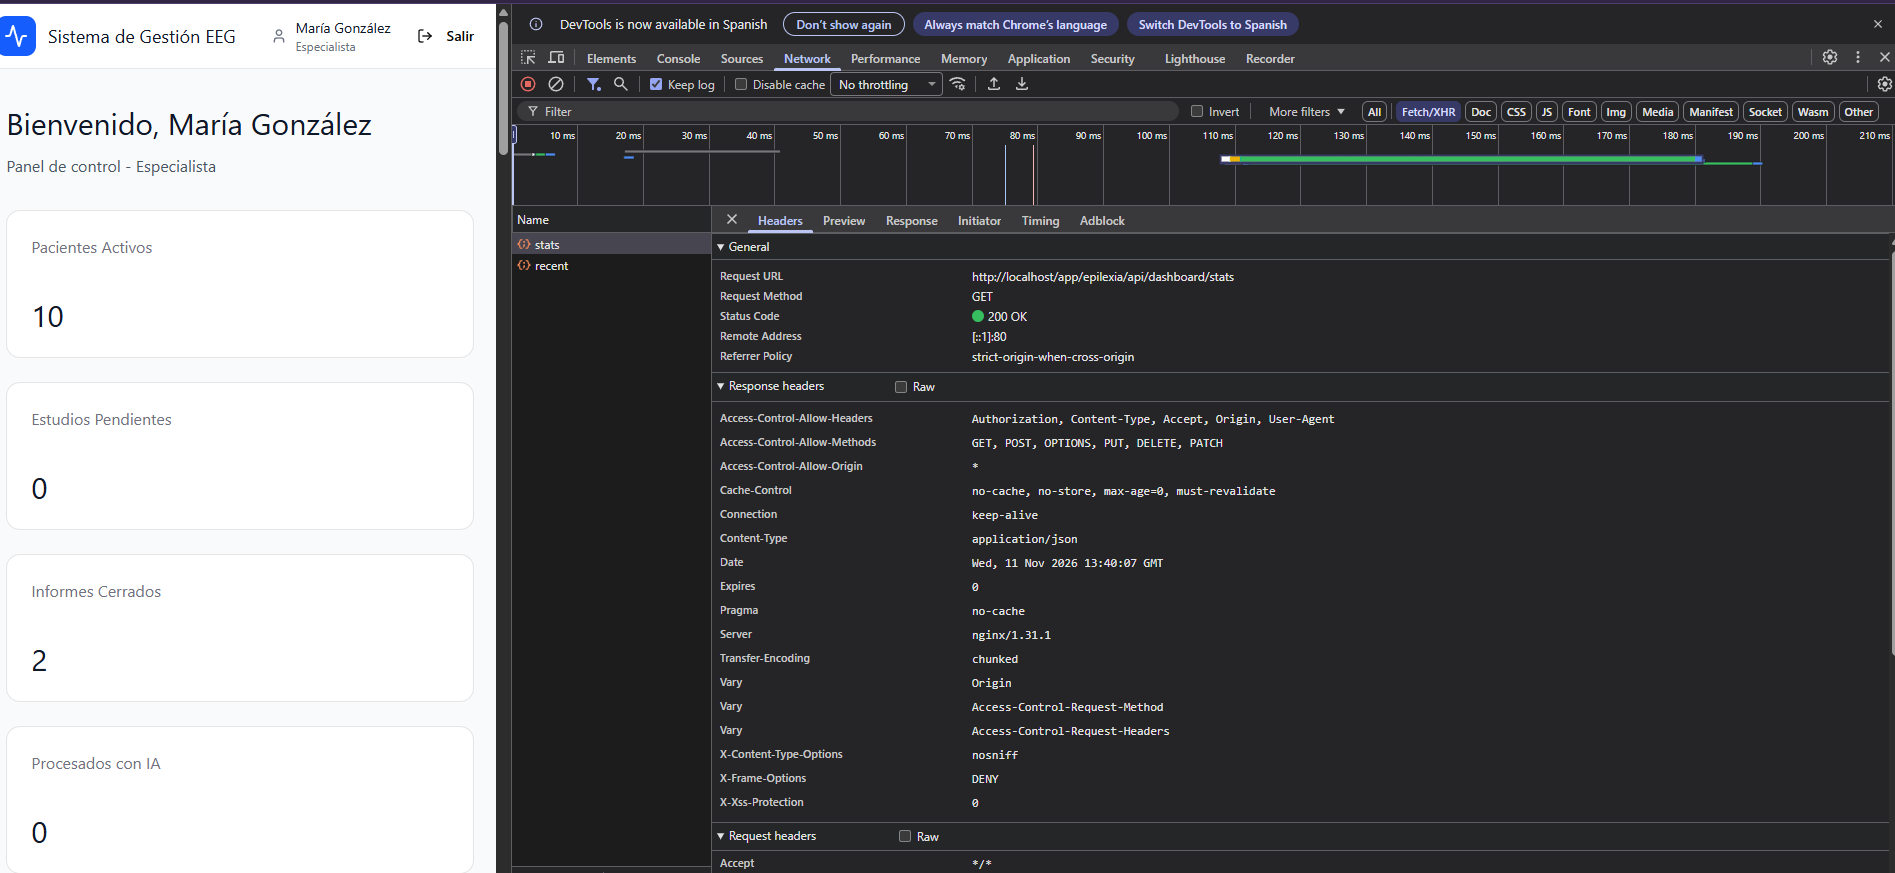
\includegraphics[width=0.95\textwidth]{Chapter6/Chapter6Figs/PI01_Dashboard_HTTP200.png}
    \caption{Acceso al panel de control de EpilexIA y verificación de la respuesta HTTP 200 durante una solicitud autenticada.}
    \label{fig:pi01_dashboard}
\end{figure}

% Figura 6.33: Encabezado Authorization Bearer
\begin{figure}[htbp]
    \centering
    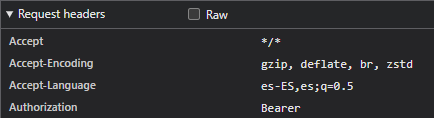
\includegraphics[width=0.75\textwidth]{Chapter6/Chapter6Figs/PI01_Authorization_Bearer.png}
    \caption{Verificación del encabezado de autorización Bearer en una solicitud autenticada mediante JWT.}
    \label{fig:pi01_authorization}
\end{figure}

% Figura 6.34: Registro de sesión en PostgreSQL
\begin{figure}[htbp]
    \centering
    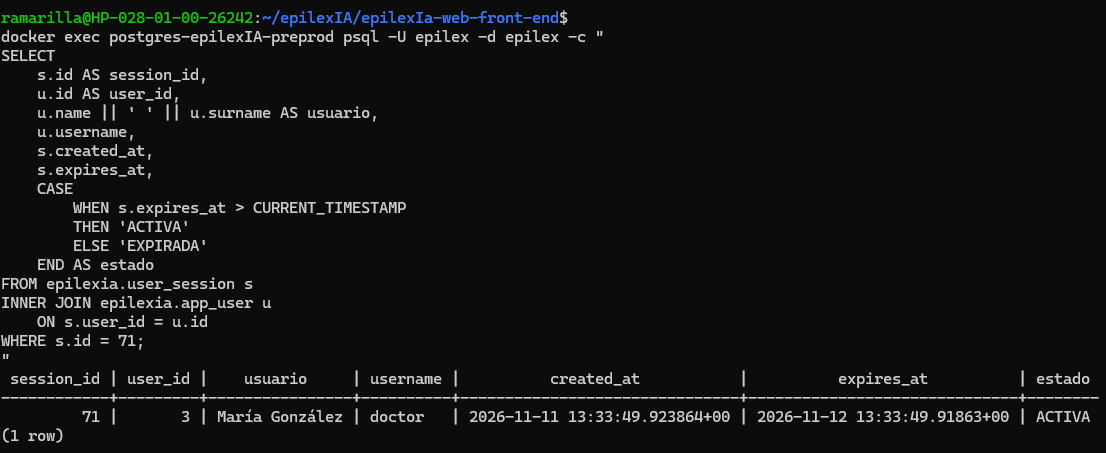
\includegraphics[width=0.95\textwidth]{Chapter6/Chapter6Figs/PI01_Sesion_PostgreSQL.png}
    \caption{Verificación del registro de sesión activa de la usuaria autenticada en PostgreSQL.}
    \label{fig:pi01_postgresql}
\end{figure}

% Impedir que las figuras se desplacen más allá
% de la conclusión de PI-01
\FloatBarrier

\Needspace{8\baselineskip}
\noindent\textbf{Resultado de la prueba:} Aprobada.

Se comprobó el funcionamiento integrado de los componentes React, Spring Boot y PostgreSQL en el escenario de autenticación con credenciales válidas. Los resultados evidenciaron el acceso al panel de control, la utilización de un \textit{token} JWT para acceder a un recurso protegido y el registro de la sesión correspondiente en la base de datos.

El alcance de esta ejecución se limitó al escenario de autenticación válida, sin incluir la evaluación de credenciales incorrectas, \textit{tokens} expirados o intentos de acceso no autorizado.


% ==================================================
% PI-02: Rechazo de solicitud sin autenticación
% ==================================================

\subsubsection{Ejecución de la prueba PI-02: Rechazo de solicitud sin autenticación}

La prueba de integración PI-02 tuvo como objetivo verificar que el \textit{backend} de EpilexIA restringe el acceso a los recursos protegidos cuando una solicitud HTTP no contiene credenciales de autenticación. Asimismo, se evaluó el comportamiento de la interfaz web ante un intento de acceso directo al panel de control sin una sesión autenticada.

Para la primera verificación, se utilizó la herramienta de línea de comandos \texttt{curl} desde el entorno local de pruebas. Se realizó una solicitud HTTP de tipo GET al \textit{endpoint} \texttt{/epilexia/api/dashboard/stats}, sin incorporar el encabezado \texttt{Authorization} ni proporcionar un \textit{token} JWT.

El servidor respondió con el código HTTP \texttt{401 Unauthorized} y un mensaje en formato JSON que indicaba que el usuario debía iniciar sesión. La respuesta no contenía las estadísticas solicitadas, lo que permitió comprobar el rechazo de la petición no autenticada.

Posteriormente, se abrió una ventana privada del navegador y se intentó acceder directamente a la dirección \texttt{http://localhost/app/dashboard}, sin iniciar sesión previamente. La aplicación redirigió automáticamente al formulario de autenticación, ubicado en \texttt{http://localhost/app/login}, impidiendo la visualización del panel de control.

El Cuadro~\ref{tab:pi02_resultados} presenta los resultados obtenidos durante ambas verificaciones.

\begin{table}[htbp]
    \centering
    \caption{Resultados de la prueba de integración PI-02.}
    \label{tab:pi02_resultados}
    \small
    \begin{tabular}{|p{0.48\textwidth}|p{0.36\textwidth}|}
        \hline
        \textbf{Verificación realizada} & \textbf{Resultado obtenido} \\
        \hline
        Solicitud HTTP sin \textit{token} JWT & Realizada sin credenciales \\
        \hline
        Respuesta del \textit{backend} & \textit{401 Unauthorized} \\
        \hline
        Mensaje de autenticación requerida & Confirmado \\
        \hline
        Entrega de estadísticas del panel de control & No se entregaron \\
        \hline
        Acceso directo al panel de control sin sesión & Redirigido al inicio de sesión \\
        \hline
        Visualización del panel protegido & Impedida \\
        \hline
    \end{tabular}
\end{table}

Como evidencia de la primera verificación, la Figura~\ref{fig:pi02_http401} muestra la respuesta HTTP 401 obtenida al consultar el \textit{endpoint} protegido sin proporcionar credenciales de autenticación.

Por su parte, la Figura~\ref{fig:pi02_redireccion} presenta la redirección al formulario de inicio de sesión después de intentar acceder directamente al panel de control sin una sesión autenticada.

% --------------------------------------------------
% Evidencias de PI-02
% --------------------------------------------------

% Figura 1: Respuesta HTTP 401
\begin{figure}[htbp]
    \centering
    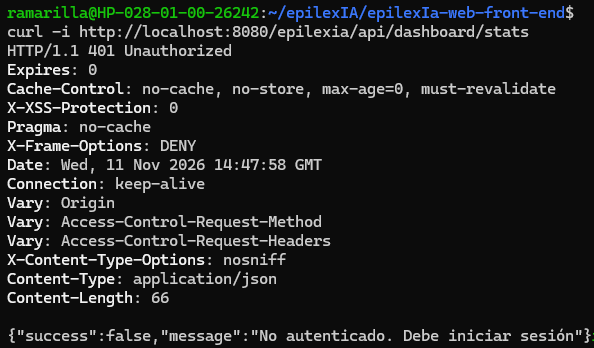
\includegraphics[width=0.90\textwidth]{Chapter6/Chapter6Figs/PI02_HTTP401.png}
    \caption{Rechazo de una solicitud HTTP sin autenticación por parte del \textit{backend} de EpilexIA.}
    \label{fig:pi02_http401}
\end{figure}

% Figura 2: Redirección al formulario de inicio de sesión
\begin{figure}[htbp]
    \centering
    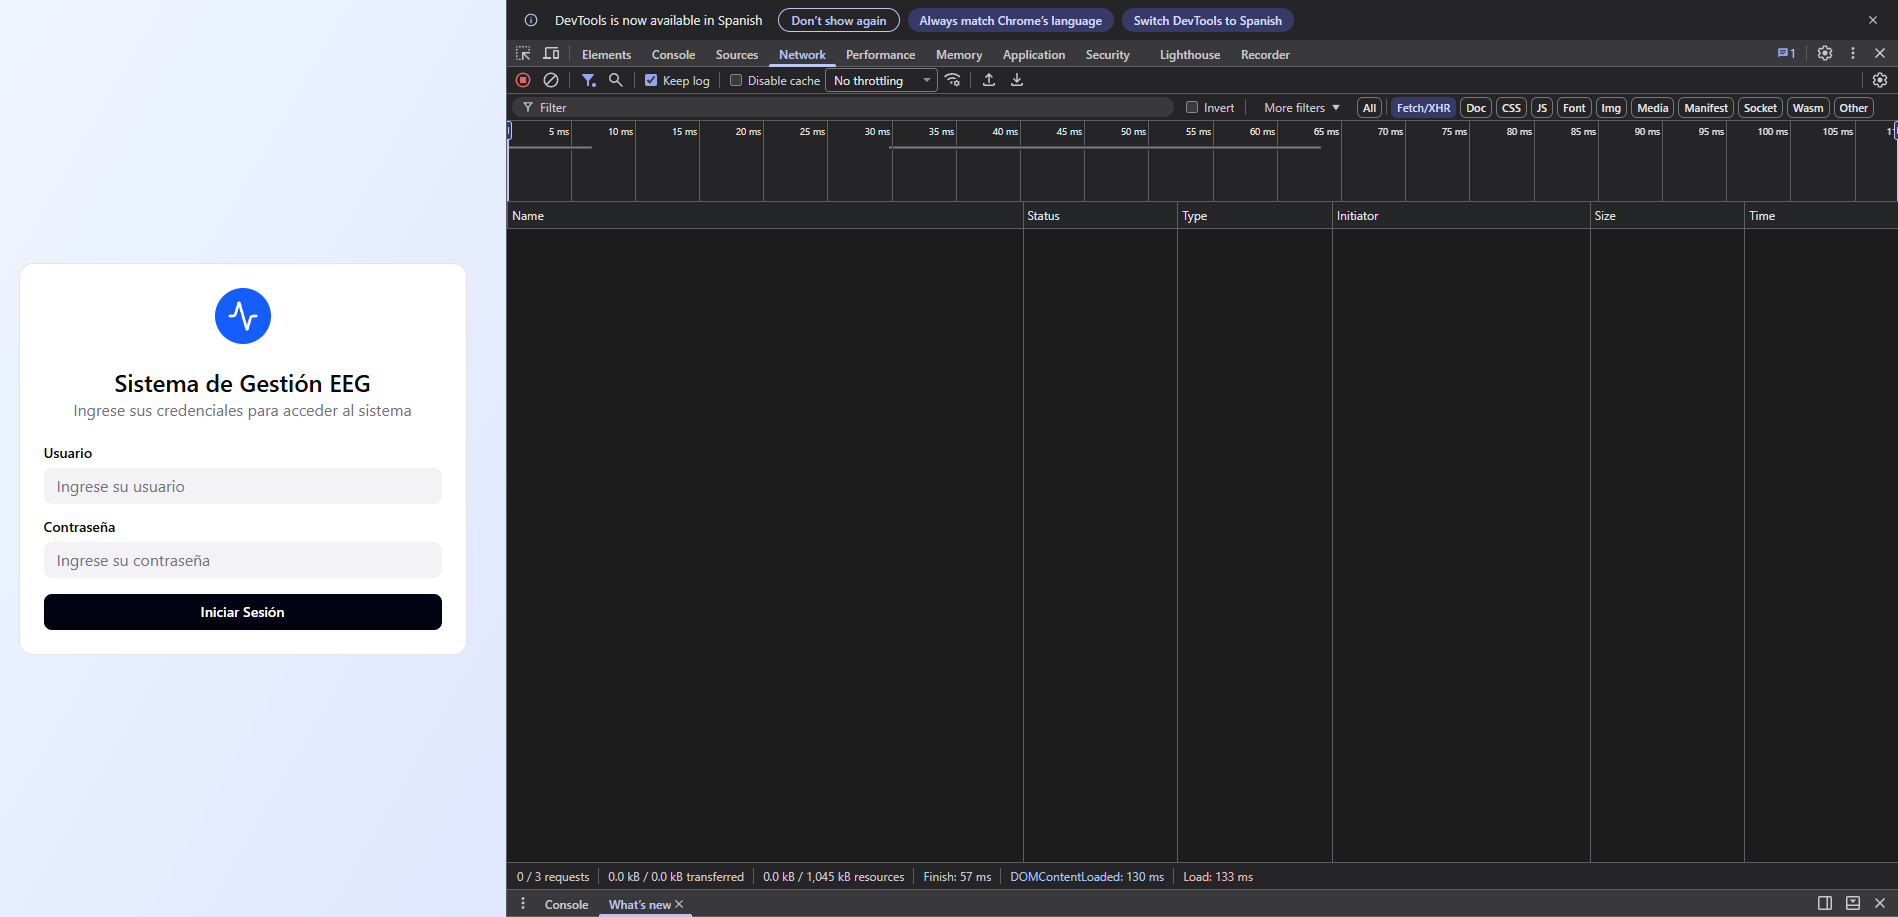
\includegraphics[width=0.95\textwidth]{Chapter6/Chapter6Figs/PI02_Redireccion_Login.png}
    \caption{Redirección al formulario de inicio de sesión ante un intento de acceso no autenticado al panel de control.}
    \label{fig:pi02_redireccion}
\end{figure}

% Mantener las evidencias antes de la conclusión
\FloatBarrier

\Needspace{8\baselineskip}
\noindent\textbf{Resultado de la prueba:} Aprobada.

Se comprobó que el \textit{backend} de EpilexIA rechazó una solicitud HTTP sin credenciales mediante el código \textit{401 Unauthorized}, sin proporcionar información del recurso protegido. Asimismo, se verificó que la interfaz web redirigió al formulario de inicio de sesión cuando se intentó acceder directamente al panel de control sin autenticación.

Los resultados evidenciaron el funcionamiento de los mecanismos de protección de acceso en los escenarios evaluados. El alcance de esta prueba se limitó a solicitudes sin credenciales y al acceso directo sin sesión, sin incluir la evaluación de \textit{tokens} inválidos o expirados.


% ==================================================
% PI-03: Revocación de sesiones
% ==================================================

\subsubsection[Ejecución de PI-03: Revocación de sesiones]{Ejecución de la prueba PI-03: Revocación de sesiones}

La prueba de integración PI-03 tuvo como objetivo verificar que el \textit{backend} de EpilexIA restringe el acceso a los recursos protegidos después del cierre de sesión de un usuario autenticado. Para ello, se evaluó el comportamiento del servidor ante solicitudes HTTP realizadas con un mismo \textit{token} JWT, antes y después de ejecutar el procedimiento de cierre de sesión.


\Needspace{7\baselineskip}

Para la primera verificación, se utilizó la herramienta
de línea de comandos \texttt{curl}, mediante un archivo
de prueba denominado \texttt{pi03\_solicitud.txt}.
Este archivo contenía una solicitud HTTP de tipo GET
dirigida al siguiente recurso protegido:

\begin{center}
\path{/epilexia/api/dashboard/stats}
\end{center}

La solicitud incorporó un \textit{token} JWT en el encabezado
\texttt{Authorization}.


Inicialmente, se ejecutó la solicitud mientras la sesión del usuario permanecía activa. El servidor respondió con el código HTTP \texttt{200 OK}, lo que permitió comprobar que las credenciales utilizadas eran aceptadas para acceder al recurso protegido.

Posteriormente, se realizó el cierre de sesión desde la interfaz web de EpilexIA. Inmediatamente después, se ejecutó nuevamente el mismo archivo de prueba, sin modificar el \textit{token} JWT utilizado en la solicitud inicial.

En esta segunda ejecución, el servidor devolvió el código HTTP \texttt{401 Unauthorized}, rechazando la solicitud realizada con las credenciales previamente aceptadas. Este comportamiento fue consistente con el mecanismo esperado de revocación de sesiones.

Como verificación complementaria, se consultó la tabla \texttt{epilexia.user\_session} de PostgreSQL, relacionando los registros de sesión con la tabla de usuarios del sistema. La consulta permitió identificar nueve registros históricos correspondientes al usuario examinado, incluyendo sus identificadores y las fechas de creación y expiración.

El Cuadro~\ref{tab:pi03_resultados} presenta los resultados obtenidos durante las verificaciones realizadas.

\begin{table}[htbp]
    \centering
    \caption{Resultados de la prueba de integración PI-03.}
    \label{tab:pi03_resultados}
    \small
    \begin{tabular}{|p{0.48\textwidth}|p{0.36\textwidth}|}
        \hline
        \textbf{Verificación realizada} & \textbf{Resultado obtenido} \\
        \hline
        Solicitud HTTP con sesión activa & 200 OK \\
        \hline
        Cierre de sesión desde la interfaz web & Ejecutado \\
        \hline
        Reutilización del mismo \textit{token} JWT & Confirmada \\
        \hline
        Solicitud HTTP después del cierre de sesión & \textit{401 Unauthorized} \\
        \hline
        Acceso al recurso protegido después del cierre & Rechazado \\
        \hline
        Consulta de sesiones en PostgreSQL & Realizada \\
        \hline
        Registros históricos identificados & 9 registros \\
        \hline
    \end{tabular}
\end{table}

Como evidencia de la primera verificación, la Figura~\ref{fig:pi03_http200} muestra la respuesta HTTP 200 obtenida al consultar el recurso protegido mientras la sesión del usuario permanecía activa.

La Figura~\ref{fig:pi03_http401} presenta la respuesta HTTP 401 obtenida inmediatamente después del cierre de sesión, utilizando el mismo \textit{token} JWT de la solicitud inicial.

Por su parte, la Figura~\ref{fig:pi03_postgresql} muestra los registros históricos de sesiones identificados mediante una consulta a PostgreSQL.

% --------------------------------------------------
% Evidencias de PI-03
% --------------------------------------------------

% Figura 1: Respuesta HTTP 200 antes del cierre
\begin{figure}[htbp]
    \centering
    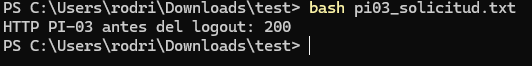
\includegraphics[width=0.90\textwidth]{Chapter6/Chapter6Figs/PI03_HTTP200_Antes.png}
    \caption{Respuesta HTTP 200 al consultar un recurso protegido antes del cierre de sesión en EpilexIA.}
    \label{fig:pi03_http200}
\end{figure}

% Figura 2: Respuesta HTTP 401 después del cierre
\begin{figure}[htbp]
    \centering
    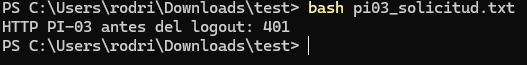
\includegraphics[width=0.90\textwidth]{Chapter6/Chapter6Figs/PI03_HTTP401_Despues.png}
    \caption{Rechazo de una solicitud HTTP realizada con el mismo \textit{token} JWT después del cierre de sesión.}
    \label{fig:pi03_http401}
\end{figure}

% Figura 3: Registros de sesiones en PostgreSQL
\begin{figure}[htbp]
    \centering
    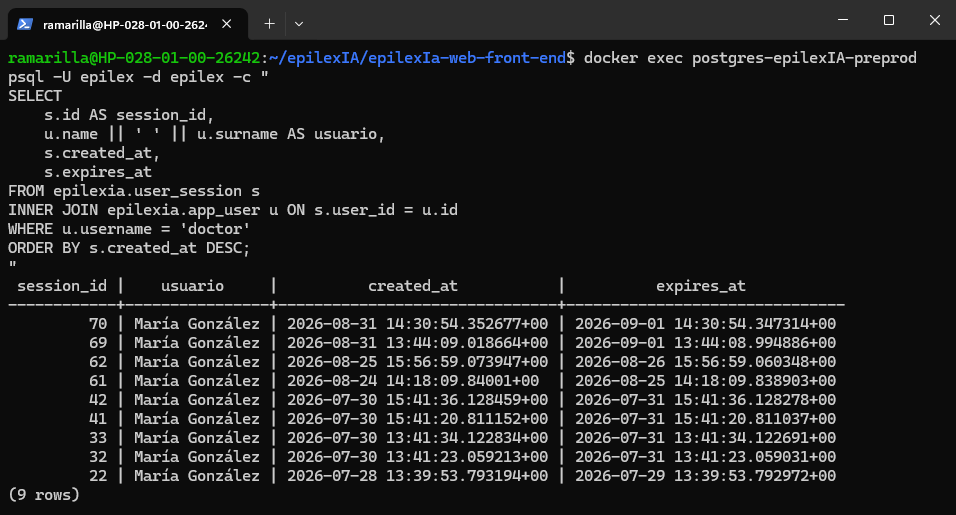
\includegraphics[width=0.95\textwidth]{Chapter6/Chapter6Figs/PI03_Sesiones_PostgreSQL.png}
    \caption{Consulta de los registros históricos de sesiones del usuario en PostgreSQL.}
    \label{fig:pi03_postgresql}
\end{figure}

% Mantener las evidencias antes de la conclusión
\FloatBarrier

\clearpage

\noindent\textbf{Resultado de la prueba:} Aprobada.

Se comprobó que el \textit{backend} de EpilexIA aceptó inicialmente una solicitud HTTP autenticada mediante el código 200 OK y rechazó una segunda solicitud realizada inmediatamente después del cierre de sesión, utilizando el mismo \textit{token} JWT, mediante el código \textit{401 Unauthorized}.

Los resultados fueron consistentes con el funcionamiento esperado del mecanismo de revocación de sesiones. La consulta a PostgreSQL complementó la documentación al permitir examinar los registros históricos persistidos. No obstante, esta consulta no permitió determinar directamente el estado de revocación de cada sesión.

El alcance de la prueba se limitó a verificar el comportamiento de un \textit{token} previamente aceptado después del cierre de sesión, sin incluir escenarios de cierre simultáneo de múltiples sesiones o revocación administrativa.


\subsubsection{Ejecución de la prueba PI-04: Persistencia de pacientes}
\label{sec:pi04-persistencia-pacientes}

Esta prueba tuvo como objetivo verificar la correcta persistencia de los datos de un paciente registrado mediante la interfaz web de EpilexIA. Se evaluó el proceso de creación del registro, la confirmación de la operación por parte del sistema y la posterior recuperación de la información almacenada en la base de datos PostgreSQL.

Para su ejecución, se accedió al módulo de estudios EEG y se seleccionó la opción de crear un nuevo estudio. Desde el apartado correspondiente al paciente, se abrió el formulario de registro y se ingresaron datos ficticios, utilizando el documento de identidad \texttt{TESTPI04001}, el nombre \texttt{Prueba} y el apellido \texttt{Integracion}. También se completaron la fecha de nacimiento (16/06/1990), el género masculino y los campos de ubicación geográfica correspondientes al departamento Central, la ciudad de Areguá y el barrio Jukyry. En el campo de notas se indicó que se trataba de un paciente ficticio utilizado para la prueba PI-04.

La Figura~\ref{fig:pi04-registro-paciente} presenta el formulario con los datos utilizados durante la ejecución de la prueba.

\begin{figure}[htbp]
    \centering
    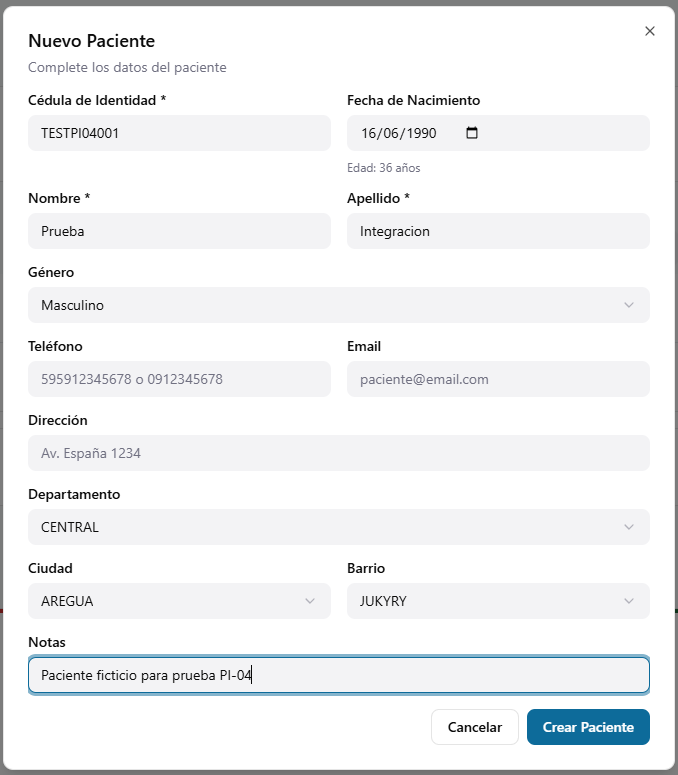
\includegraphics[width=0.72\textwidth]{Chapter6/Chapter6Figs/PI04_registro_paciente.png}
    \caption{Formulario de registro de un paciente ficticio en EpilexIA.}
    \label{fig:pi04-registro-paciente}
\end{figure}
\FloatBarrier

Una vez completados los campos requeridos, se ejecutó la operación de creación del paciente. El sistema mostró una notificación de confirmación con el mensaje \textit{Paciente creado} y seleccionó automáticamente el registro recién creado en el formulario de nuevo estudio EEG. Este comportamiento permitió comprobar que el paciente quedó disponible para su utilización en el proceso de registro de estudios.

La Figura~\ref{fig:pi04-confirmacion-paciente} muestra la confirmación de la operación y la selección automática del paciente.

\begin{figure}[htbp]
    \centering
    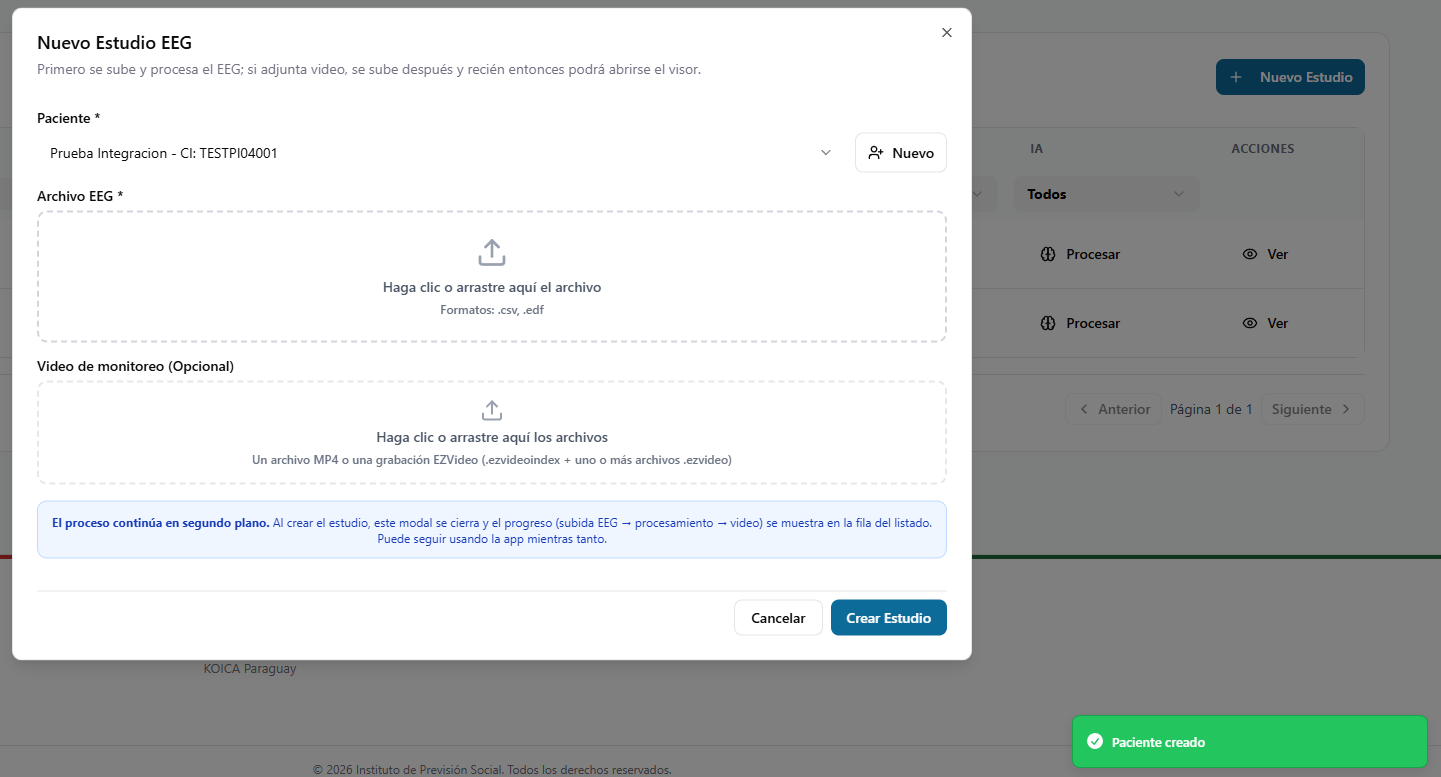
\includegraphics[width=0.90\textwidth]{Chapter6/Chapter6Figs/PI04_confirmacion_paciente.png}
    \caption{Confirmación del registro y selección automática del paciente en el formulario de nuevo estudio EEG.}
    \label{fig:pi04-confirmacion-paciente}
\end{figure}
\FloatBarrier

Posteriormente, se realizó una consulta SQL de solo lectura sobre la tabla \texttt{epilexia.patient} de PostgreSQL, utilizando el documento de identidad \texttt{TESTPI04001} como criterio de búsqueda. La consulta recuperó un único registro, identificado mediante el valor \texttt{id = 11}.

Se verificó que los valores almacenados coincidieran con los introducidos en el formulario, incluyendo el documento de identidad, el nombre, el apellido, la fecha de nacimiento, el género, el departamento, la ciudad, el barrio y las notas del paciente. Asimismo, se constató que el sistema registró la fecha y hora de creación mediante el campo \texttt{created\_at}.

La Figura~\ref{fig:pi04-persistencia-postgresql} presenta el resultado de la consulta SQL utilizada para comprobar la persistencia de la información.

\begin{figure}[htbp]
    \centering
    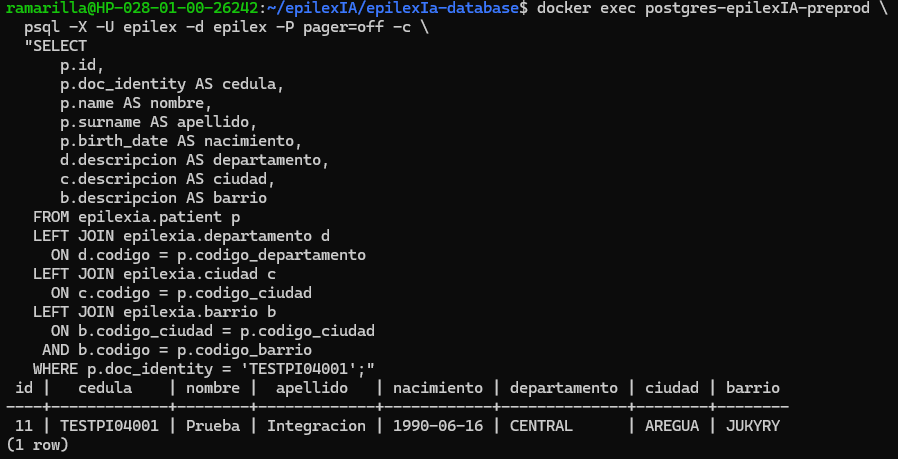
\includegraphics[width=\textwidth]{Chapter6/Chapter6Figs/PI04_persistencia_postgresql.png}
    \caption{Verificación de la persistencia de los datos del paciente mediante una consulta SQL a PostgreSQL.}
    \label{fig:pi04-persistencia-postgresql}
\end{figure}
\FloatBarrier

La prueba se clasificó como aprobada. El sistema permitió registrar correctamente al paciente ficticio, confirmó la operación mediante la interfaz web y conservó la información en PostgreSQL, desde donde fue posible recuperarla y verificar su correspondencia con los datos ingresados.

Por consiguiente, la prueba PI-04 se considera aprobada, al comprobarse satisfactoriamente el registro y la persistencia de los datos del paciente en la base de datos del sistema.


\subsubsection{Ejecución de la prueba PI-05: Registro de estudios y archivos EEG}

Esta prueba tuvo como objetivo verificar el correcto registro de estudios electroencefalográficos en EpilexIA, incluyendo la asociación con un paciente previamente registrado, la carga y el procesamiento de un archivo EEG y la persistencia de la información correspondiente en la base de datos PostgreSQL. Asimismo, se evaluó la disponibilidad de las señales electroencefalográficas en el visualizador del sistema una vez finalizado el procesamiento.

Para su ejecución, se accedió al módulo de estudios EEG y se seleccionó la opción de crear un nuevo estudio. Se utilizó el paciente ficticio Prueba Integracion, identificado mediante el documento de identidad TESTPI04001, registrado previamente durante la prueba PI-04. Posteriormente, se seleccionó el archivo \texttt{Prueba Integracion 2025-04-07 07-04-59.edf}, con un tamaño aproximado de 180 MiB. No se adjuntó un archivo de video, debido a que este componente es opcional y no formaba parte del alcance de la presente prueba.

Antes de iniciar el registro, el sistema ejecutó las validaciones correspondientes y mostró mensajes que confirmaban la compatibilidad del archivo EEG con el paciente seleccionado y la ausencia de errores bloqueantes. La Figura~\ref{fig:pi05-formulario-estudio} presenta el formulario utilizado durante esta etapa.

\begin{figure}[htbp]
    \centering
    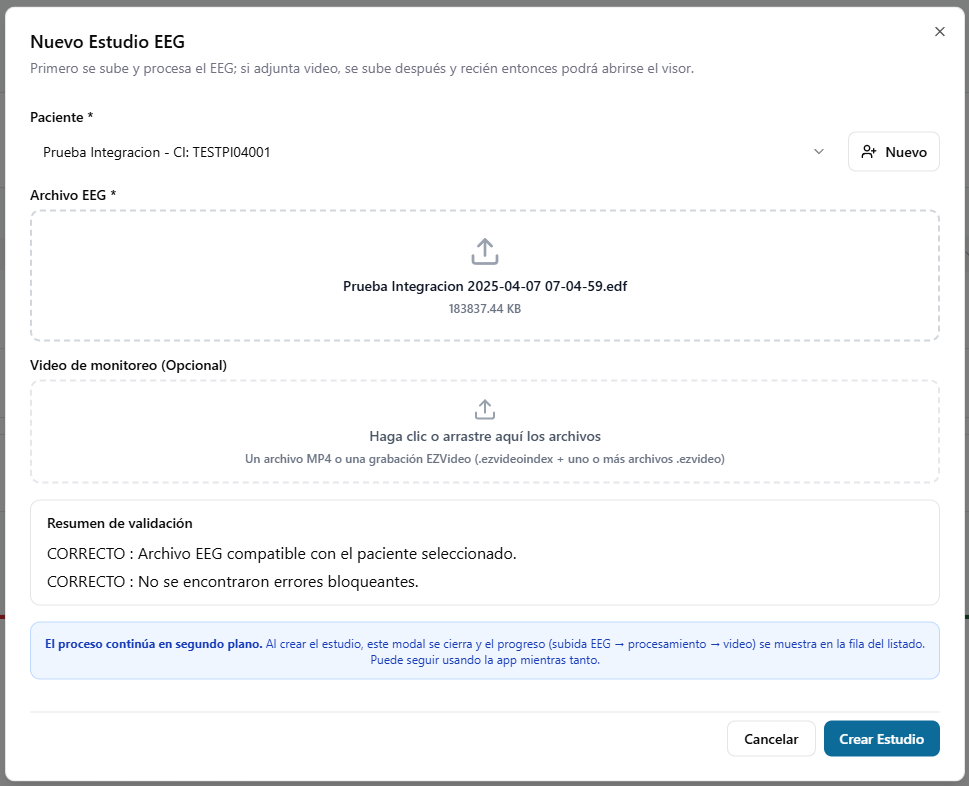
\includegraphics[width=0.90\textwidth]{Chapter6/Chapter6Figs/PI05_formulario_estudio.png}
    \caption{Formulario de registro de un estudio EEG con el paciente y el archivo seleccionados, acompañado de los resultados de validación.}
    \label{fig:pi05-formulario-estudio}
\end{figure}
\FloatBarrier

Una vez completadas las validaciones, se ejecutó la operación de creación del estudio. El sistema incorporó el nuevo registro al listado de estudios EEG e inició la carga del archivo seleccionado. Durante este procedimiento, la interfaz mostró el avance de la transferencia y, posteriormente, el estado de procesamiento, permitiendo observar la continuidad de la operación en segundo plano.

Al finalizar, el estudio apareció en el listado con el estado \emph{Procesado}, asociado al paciente Prueba Integracion y al archivo EDF correspondiente. La Figura~\ref{fig:pi05-estudio-procesado} muestra el resultado de esta operación.

\begin{figure}[htbp]
    \centering
    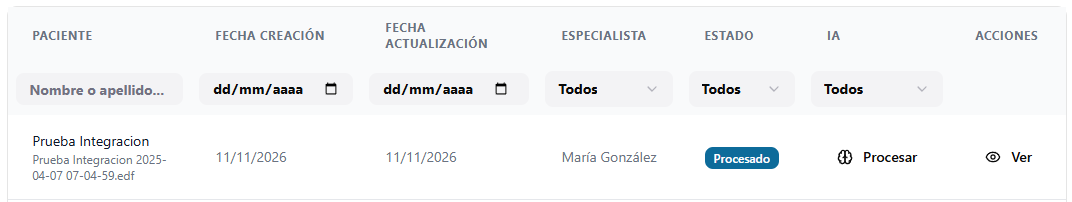
\includegraphics[width=\textwidth]{Chapter6/Chapter6Figs/PI05_estudio_procesado.png}
    \caption{Estudio EEG registrado correctamente en EpilexIA con el estado Procesado.}
    \label{fig:pi05-estudio-procesado}
\end{figure}
\FloatBarrier

Posteriormente, se accedió al estudio mediante la opción de visualización disponible en el listado. El sistema permitió abrir el visualizador EEG y representar gráficamente las señales electroencefalográficas contenidas en el archivo procesado. Se observaron los trazados correspondientes a los distintos canales, sus identificadores, las referencias temporales y los elementos de navegación del registro.

La Figura~\ref{fig:pi05-visualizador-eeg} presenta, a modo ilustrativo, la visualización de las señales de un estudio EEG procesado en la plataforma. Esta comprobación permitió verificar que los datos del archivo EEG se encontraban disponibles para su representación gráfica mediante la interfaz del sistema.

\begin{figure}[htbp]
    \centering
    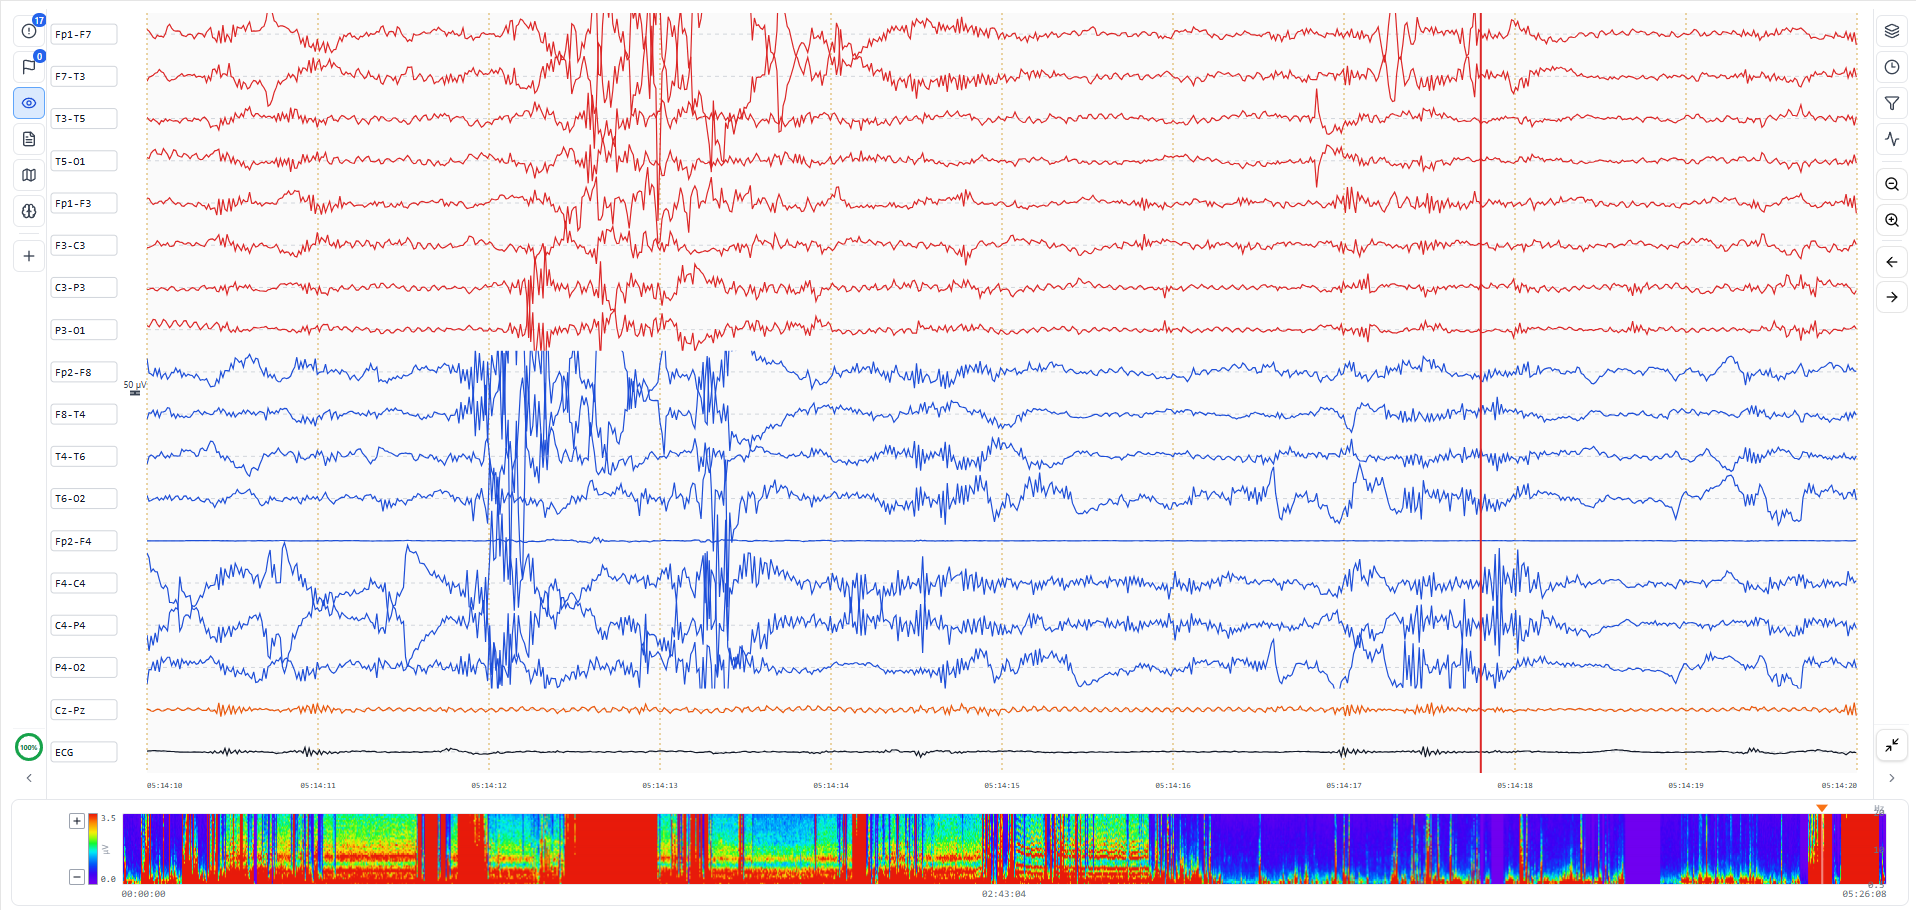
\includegraphics[width=\textwidth]{Chapter6/Chapter6Figs/PI05_visualizador_eeg.png}
    \caption{Visualización de las señales electroencefalográficas de un estudio EEG procesado en EpilexIA.}
    \label{fig:pi05-visualizador-eeg}
\end{figure}
\FloatBarrier

Finalmente, se realizó una consulta SQL de solo lectura sobre las tablas \texttt{epilexia.study}, \texttt{epilexia.patient} y \texttt{epilexia.study\_file} de PostgreSQL, con el propósito de comprobar la persistencia de la información del estudio y los metadatos del archivo asociado.

La consulta recuperó un único registro correspondiente al estudio con identificador \texttt{id = 3}, asociado al paciente con documento de identidad TESTPI04001. Se verificó que el estado almacenado era \emph{Procesado} y que el nombre del archivo coincidía con el seleccionado durante el registro.

Asimismo, se comprobó el almacenamiento de los metadatos del archivo EEG, incluyendo un tamaño de 188\,249\,536 bytes, una duración de 19\,568 segundos y una frecuencia de muestreo de 250 Hz. La Figura~\ref{fig:pi05-persistencia-postgresql} presenta el resultado de la consulta SQL utilizada para esta verificación.

\begin{figure}[htbp]
    \centering
    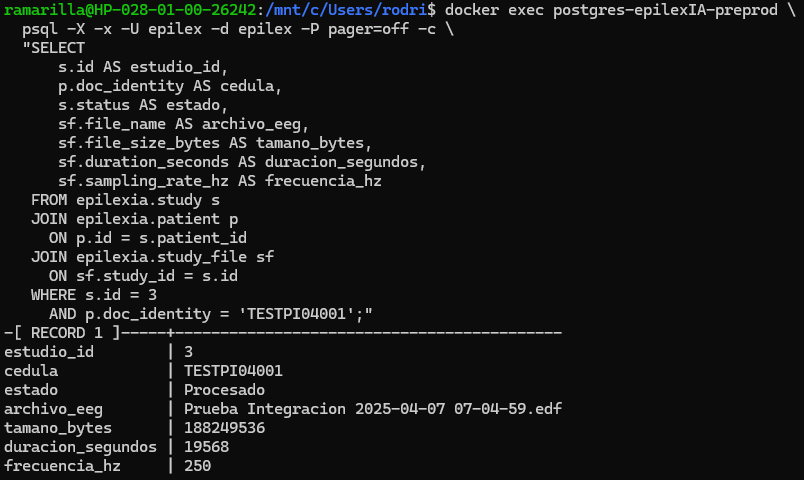
\includegraphics[width=0.90\textwidth]{Chapter6/Chapter6Figs/PI05_persistencia_postgresql.png}
    \caption{Verificación de la persistencia del estudio EEG y los metadatos del archivo asociado mediante una consulta SQL a PostgreSQL.}
    \label{fig:pi05-persistencia-postgresql}
\end{figure}
\FloatBarrier

La prueba PI-05 se clasificó como aprobada.
El sistema permitió registrar un estudio EEG asociado a un paciente existente, cargar y procesar un archivo en formato EDF, presentar el estado final de la operación y visualizar las señales electroencefalográficas correspondientes.
Adicionalmente, la consulta a PostgreSQL confirmó la persistencia del registro del estudio y de los metadatos del archivo asociado.

Estas verificaciones comprueban la integración entre la interfaz web, los componentes responsables del registro y procesamiento de archivos EEG y la base de datos, así como la recuperación y la representación gráfica de las señales.
No constituyen una evaluación exhaustiva de todos los formatos, configuraciones de adquisición o condiciones de procesamiento posibles, ni evalúan la exactitud diagnóstica de la interpretación de las señales.

\subsubsection{Ejecución de la prueba PI-15: Indisponibilidad del servicio de IA}
\label{subsubsec:ejecucion-pi15}

Esta prueba tuvo como objetivo verificar que la indisponibilidad temporal del servicio de inteligencia artificial no impide la carga ni la revisión de los estudios, y que no deja ejecuciones en un estado inconsistente.

La prueba se ejecutó en un entorno de pruebas local que replica el despliegue mediante los mismos contenedores, con la cola persistente \texttt{pgqueue} y el modelo HGB~2.0.
Se utilizó este entorno, y no la instancia empleada en el hospital, porque el procedimiento requiere detener un servicio de manera deliberada.
Para provocar la indisponibilidad se detuvo el contenedor de la API de inteligencia artificial, mientras los demás componentes permanecieron en funcionamiento.

Con el servicio detenido, se registró un estudio nuevo para un paciente de prueba y se cargó su archivo EDF.
El sistema completó la carga y el procesamiento del archivo, y el estudio quedó en estado Procesado, pendiente del análisis mediante IA, tal como se observa en la Figura~\ref{fig:pi15-listado-estudio-cargado}.

\begin{figure}[htbp]
    \centering
    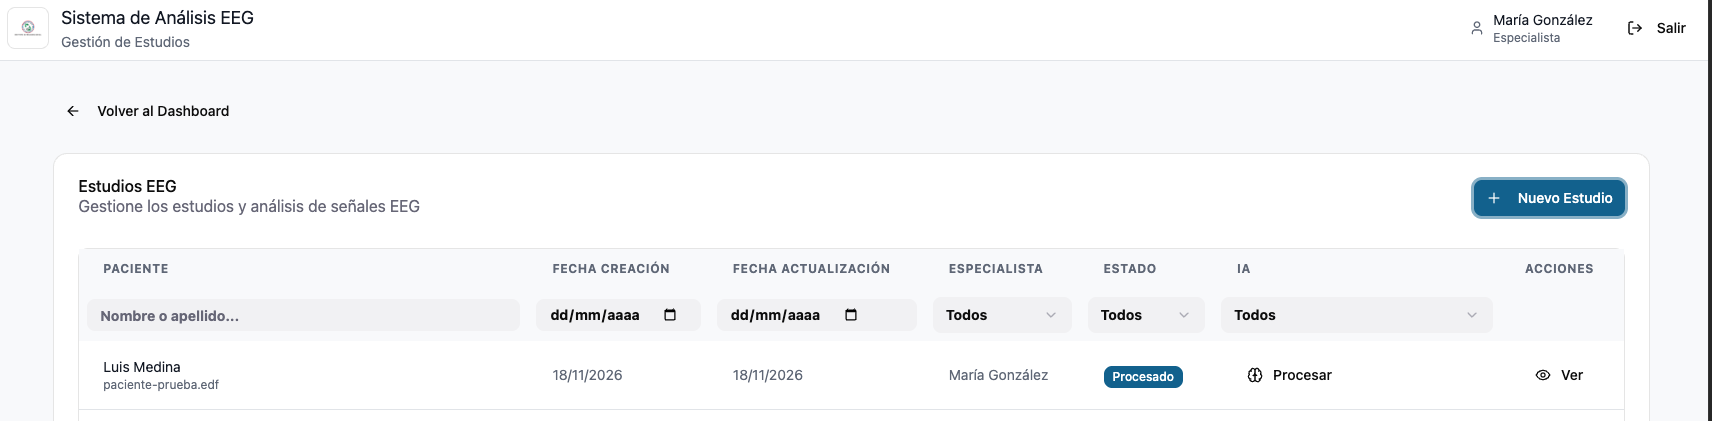
\includegraphics[width=0.90\textwidth]{Chapter6/Chapter6Figs/PI15_listado_estudio_cargado.png}
    \caption{Estudio cargado y procesado con el servicio de inteligencia artificial detenido.}
    \label{fig:pi15-listado-estudio-cargado}
\end{figure}

A continuación, se abrió el estudio en el visualizador.
Las señales se presentaron con normalidad, dado que su recuperación depende del \textit{backend} clínico y no del subsistema de IA.
El espectrograma, que sí se obtiene de dicho subsistema, no pudo generarse, y el sistema lo informó con el mensaje «No se pudo generar el espectrograma: el servicio de IA no está disponible en este momento. Reintentar más tarde.», como muestra la Figura~\ref{fig:pi15-visualizador-senales}.

\begin{figure}[htbp]
    \centering
    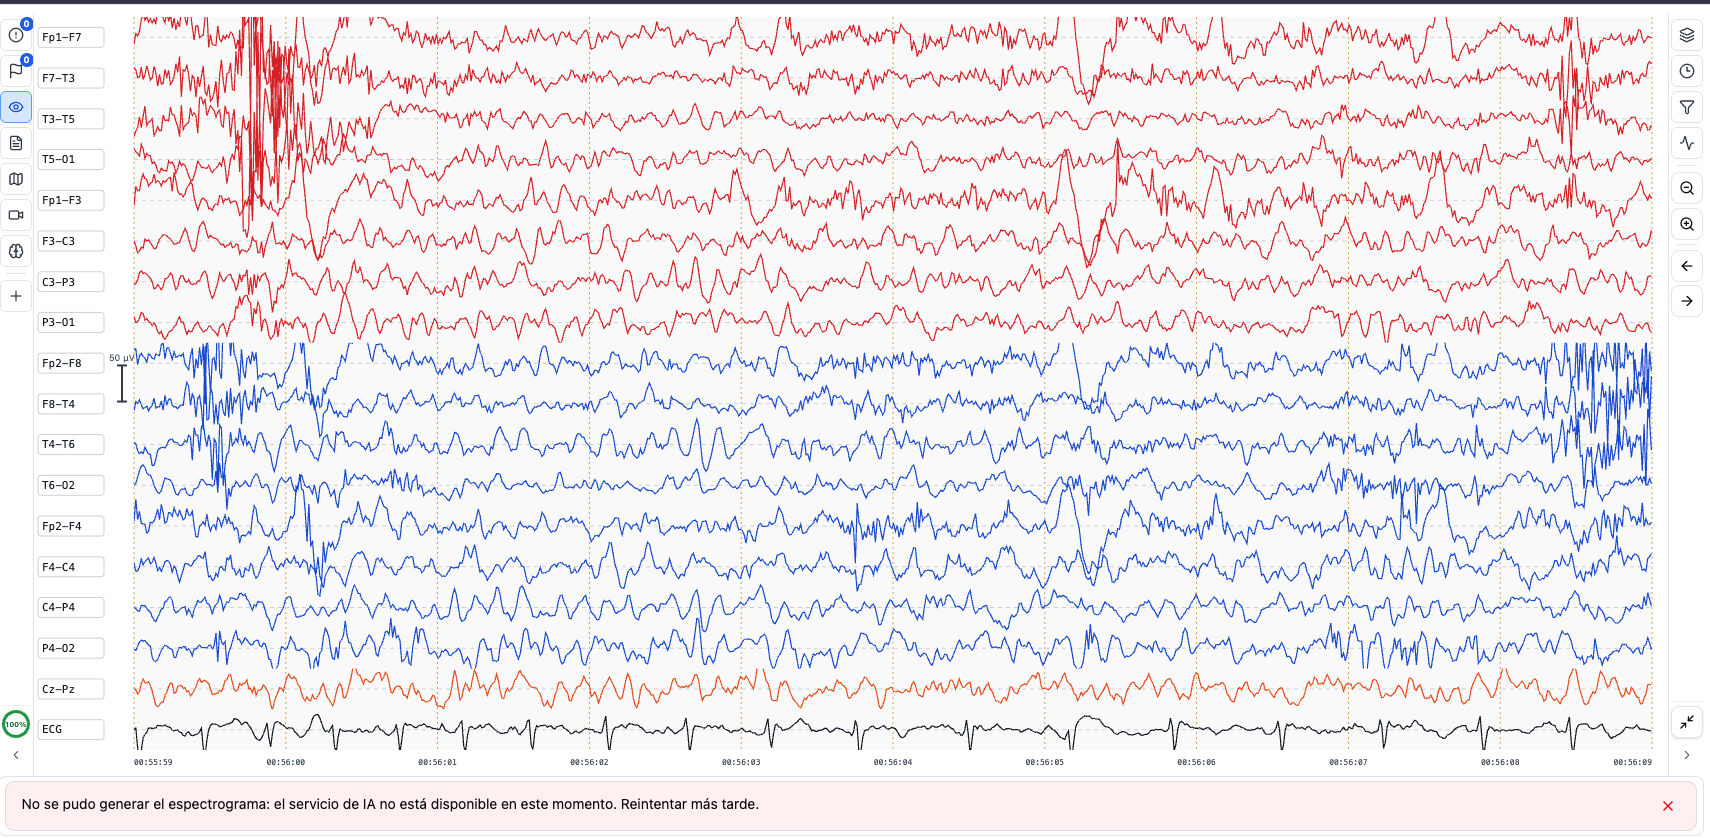
\includegraphics[width=0.90\textwidth]{Chapter6/Chapter6Figs/PI15_visualizador_senales.png}
    \caption{Visualización de las señales con el servicio de inteligencia artificial detenido y mensaje correspondiente al espectrograma.}
    \label{fig:pi15-visualizador-senales}
\end{figure}

También se abrió un estudio que había sido analizado con anterioridad.
En este caso, el panel de anomalías presentó el aviso «Anomalías detectadas por IA no disponibles», acompañado del motivo de la indisponibilidad.
De esta manera, la falta temporal de los resultados no se presenta como una ausencia de anomalías en el estudio.
La Figura~\ref{fig:pi15-estudio-previo} presenta esta situación.

\begin{figure}[htbp]
    \centering
    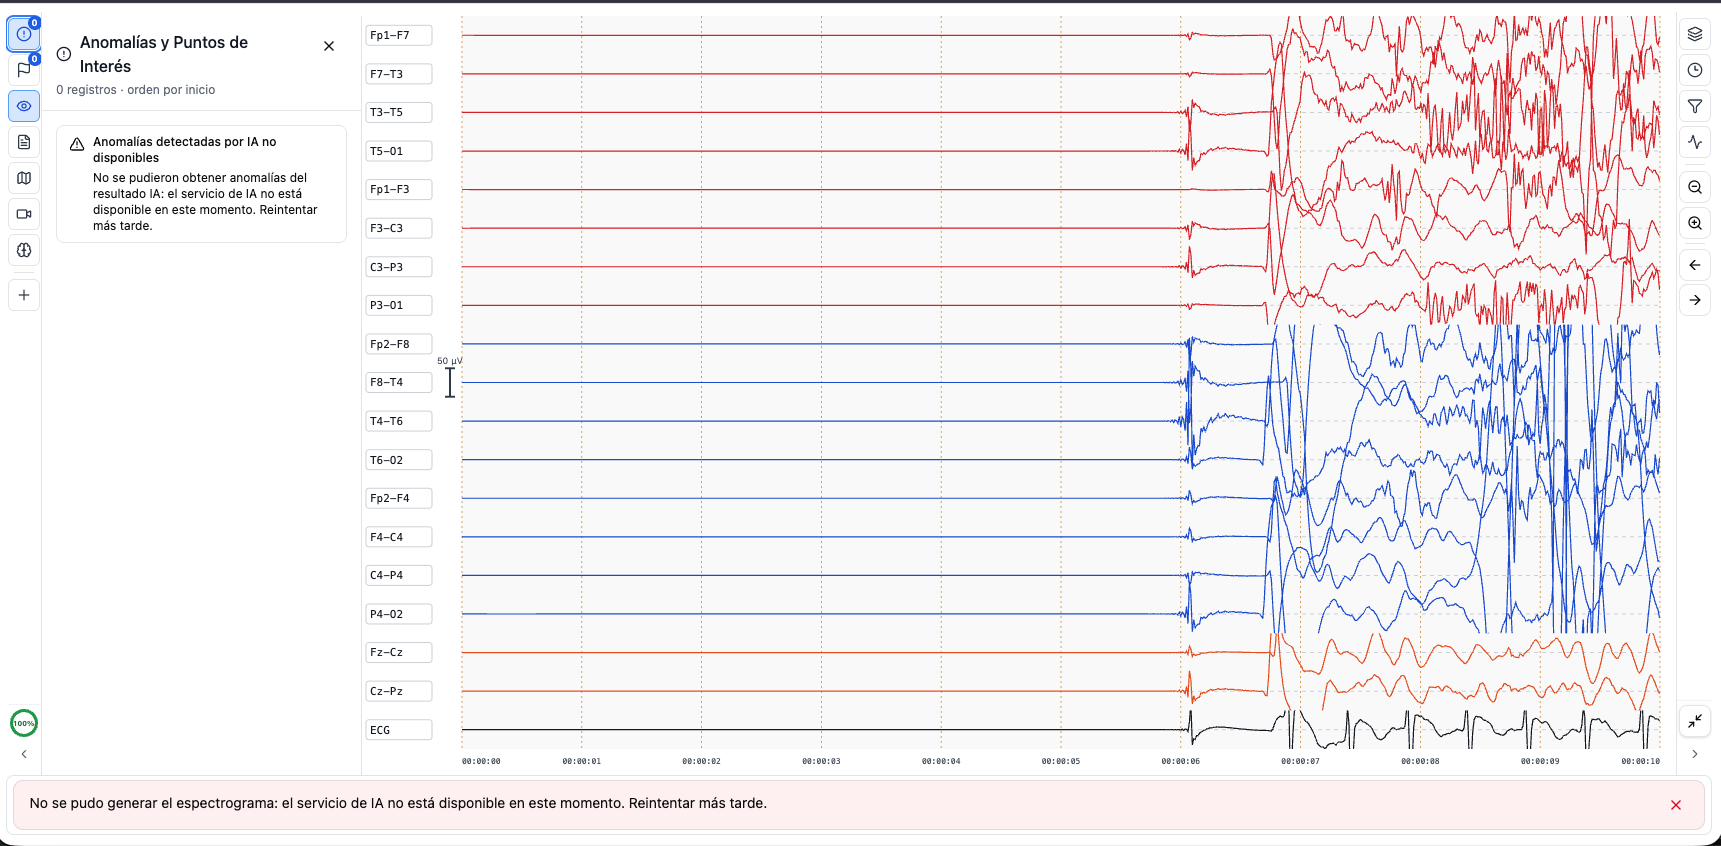
\includegraphics[width=0.90\textwidth]{Chapter6/Chapter6Figs/PI15_estudio_previo.png}
    \caption{Estudio analizado previamente, con el aviso de anomalías de IA no disponibles.}
    \label{fig:pi15-estudio-previo}
\end{figure}

Posteriormente, se solicitó de forma manual el análisis del estudio nuevo desde el listado de estudios.
El sistema respondió con el mensaje «No se pudo iniciar el análisis IA: el servicio de IA no está disponible en este momento. Reintentar más tarde.», que se observa en la Figura~\ref{fig:pi15-mensaje-inicio-manual}.

\begin{figure}[htbp]
    \centering
    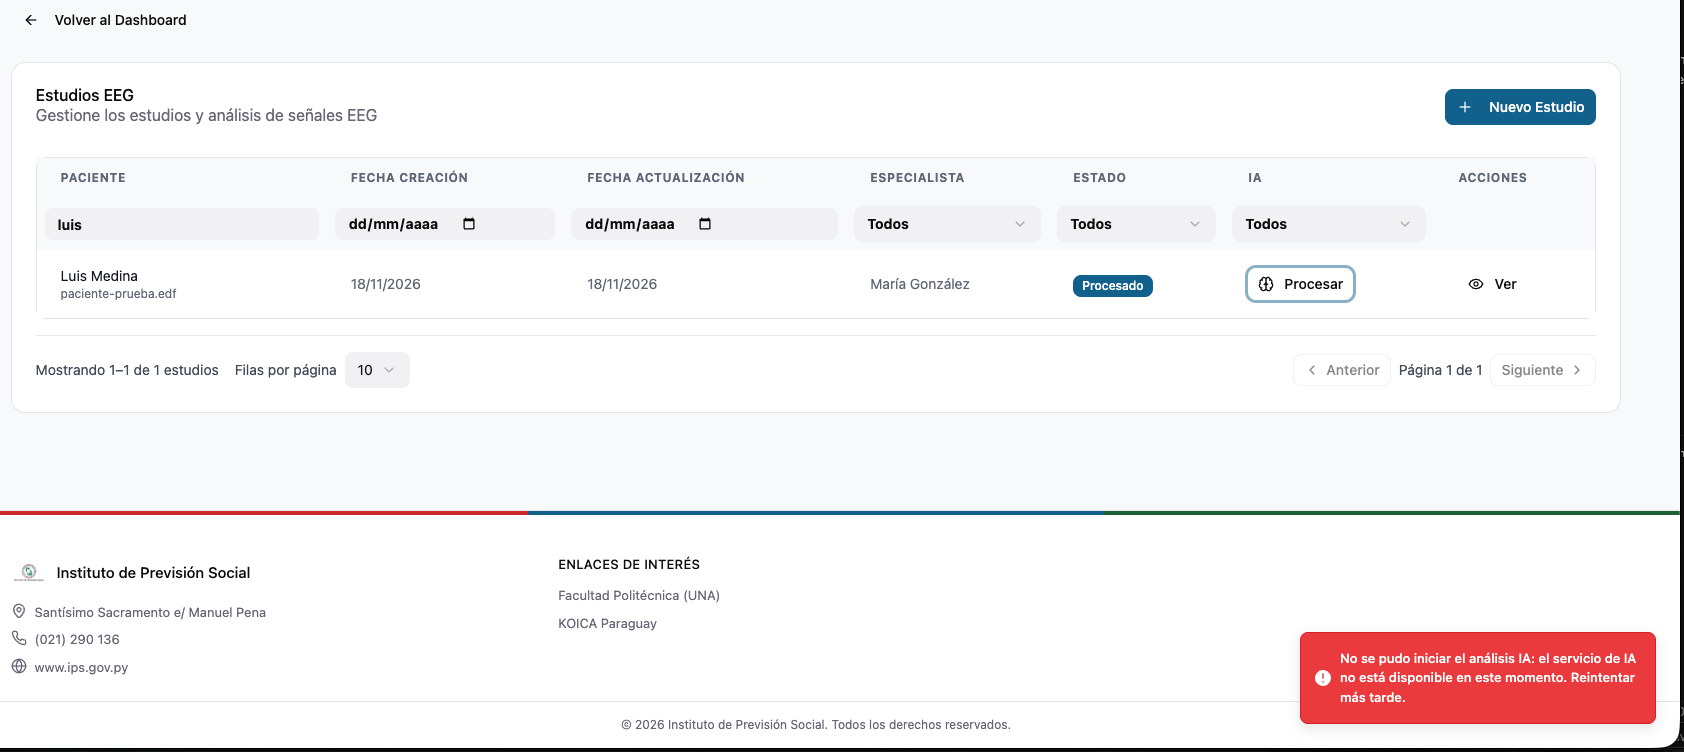
\includegraphics[width=0.90\textwidth]{Chapter6/Chapter6Figs/PI15_mensaje_inicio_manual.png}
    \caption{Mensaje presentado al solicitar el análisis con el servicio de inteligencia artificial detenido.}
    \label{fig:pi15-mensaje-inicio-manual}
\end{figure}

Durante la indisponibilidad, que se mantuvo por 49 minutos, el \textit{backend} reintentó el encolado automático del estudio cada 30 segundos y registró cada intento fallido.
Ni estos intentos ni las solicitudes manuales generaron registros de ejecución en la base de datos clínica, por lo que el estudio permaneció como pendiente de análisis, sin ejecuciones fallidas ni duplicadas.

Finalmente, se inició nuevamente el contenedor de la API de inteligencia artificial.
A los 14 segundos, el mecanismo de encolado automático registró la ejecución del estudio, sin intervención del usuario.
El motor tomó el trabajo y el análisis finalizó correctamente en 1 minuto y 36 segundos.
Al concluir, el estudio contaba con un único registro de ejecución, en estado finalizado, y el listado lo presentó con la indicación «IA listo», como se observa en la Figura~\ref{fig:pi15-listado-ia-listo}.

\begin{figure}[htbp]
    \centering
    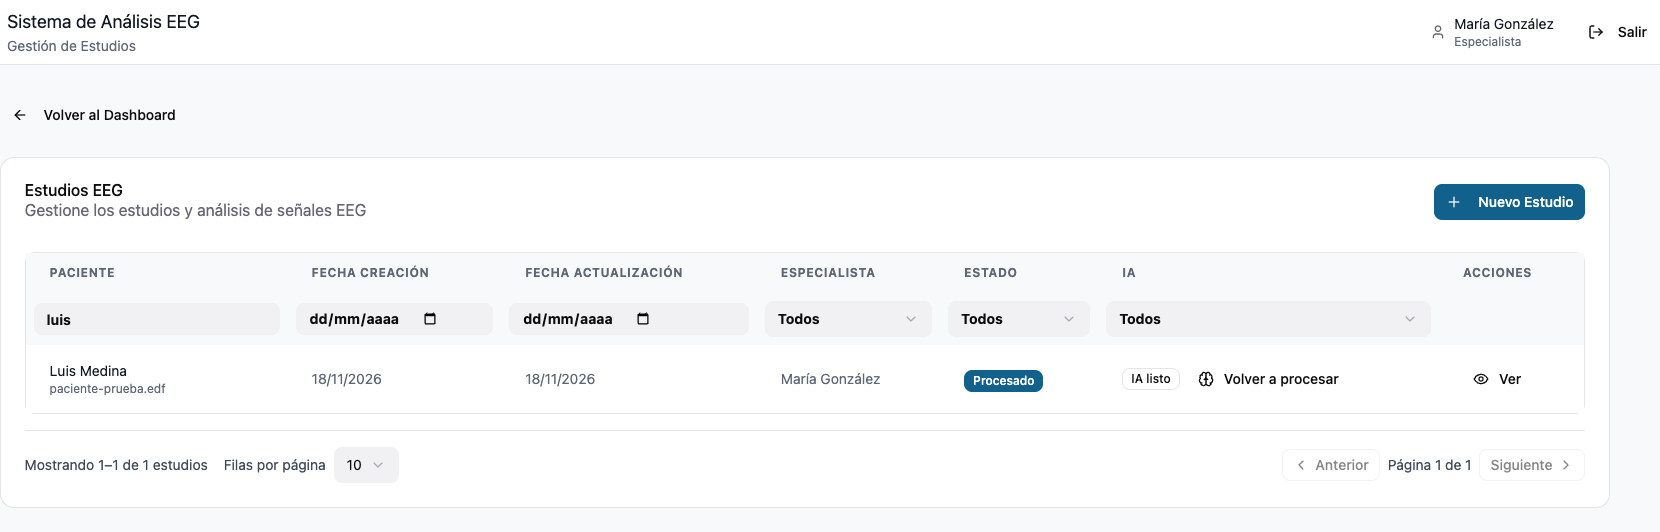
\includegraphics[width=0.90\textwidth]{Chapter6/Chapter6Figs/PI15_listado_ia_listo.png}
    \caption{Estudio con el análisis mediante IA finalizado tras el restablecimiento del servicio.}
    \label{fig:pi15-listado-ia-listo}
\end{figure}

Los resultados observados coincidieron con el comportamiento esperado para el caso PI-15, por lo que la prueba se clasificó como aprobada.
El estudio pudo cargarse y revisarse con el servicio de IA detenido, no se perdió ni quedó en un estado inconsistente, y el análisis se ejecutó de forma automática al restablecerse el servicio.

\subsubsection{Ejecución de la prueba PI-16: Saturación de la cola de procesamiento}
\label{subsubsec:ejecucion-pi16}

Esta prueba tuvo como objetivo verificar que, cuando la cola de procesamiento alcanza su límite, una solicitud adicional recibe una respuesta de error controlada y coherente entre los servicios, y que ningún estudio queda sin procesar.

La prueba se ejecutó en el mismo entorno local que la prueba PI-15.
Para alcanzar la saturación con pocos estudios, el límite de trabajos en cola, establecido en 10 en ese entorno, se redujo a 2 mediante la configuración de la API de inteligencia artificial.
Además, se detuvo el motor de procesamiento, de modo que los trabajos encolados permanecieran en espera.

En estas condiciones, se registraron tres estudios nuevos para pacientes de prueba, que quedaron en estado Procesado, como muestra la Figura~\ref{fig:pi16-listado-tres-estudios}.

\begin{figure}[htbp]
    \centering
    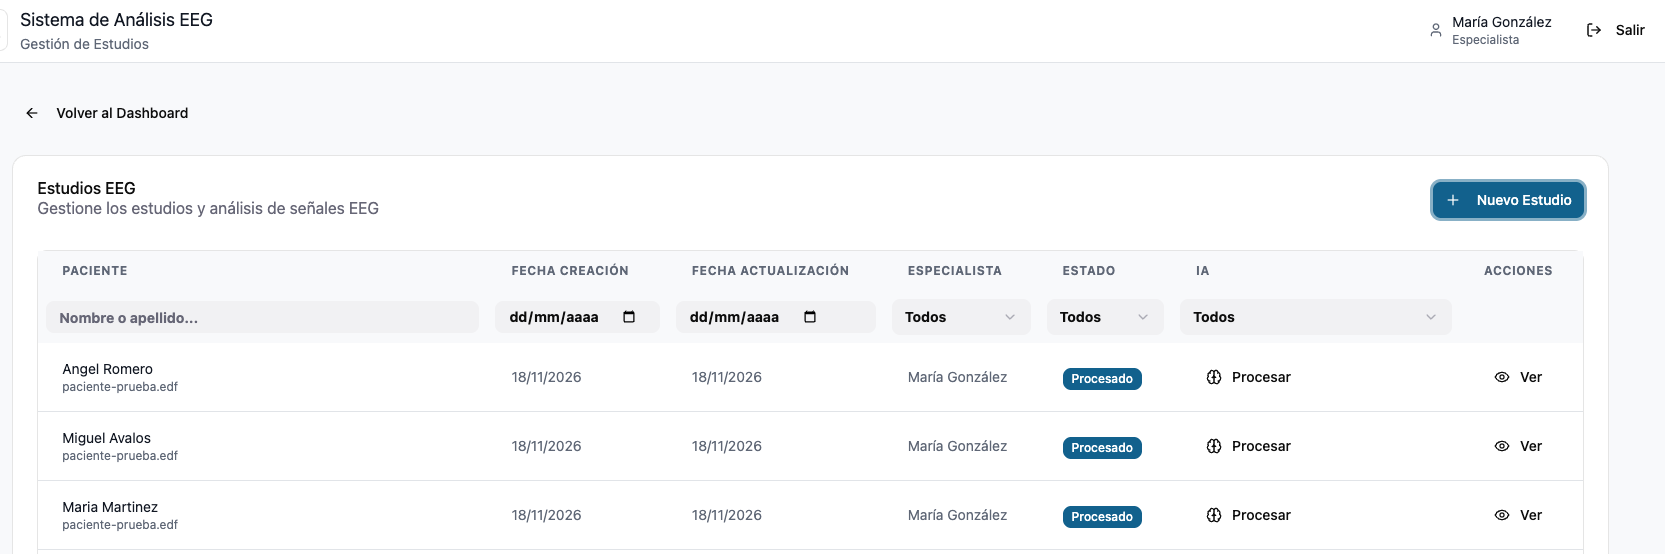
\includegraphics[width=0.90\textwidth]{Chapter6/Chapter6Figs/PI16_listado_tres_estudios.png}
    \caption{Tres estudios cargados y pendientes del análisis mediante IA.}
    \label{fig:pi16-listado-tres-estudios}
\end{figure}

El mecanismo de encolado automático registró las ejecuciones de los dos primeros estudios, con lo cual la cola alcanzó su límite.
Al intentar encolar el tercero, la API de inteligencia artificial rechazó la solicitud con el código HTTP 503 y registró la condición de cola llena.
El \textit{backend} identificó esta respuesta, interrumpió el encolado y lo reintentó en los ciclos siguientes, cada 30 segundos, con el mismo resultado.

Luego se solicitó de forma manual el análisis del tercer estudio desde el listado.
El \textit{backend} respondió con el código HTTP 503 y la interfaz presentó el mensaje «Cola de análisis IA llena; reintentar más tarde», tal como se observa en la Figura~\ref{fig:pi16-mensaje-cola-llena}.
Ni los rechazos automáticos ni el manual generaron un registro de ejecución para ese estudio en la base de datos clínica, mientras que los otros dos figuraban en cola tanto en esta base como en la del subsistema de IA.

\begin{figure}[htbp]
    \centering
    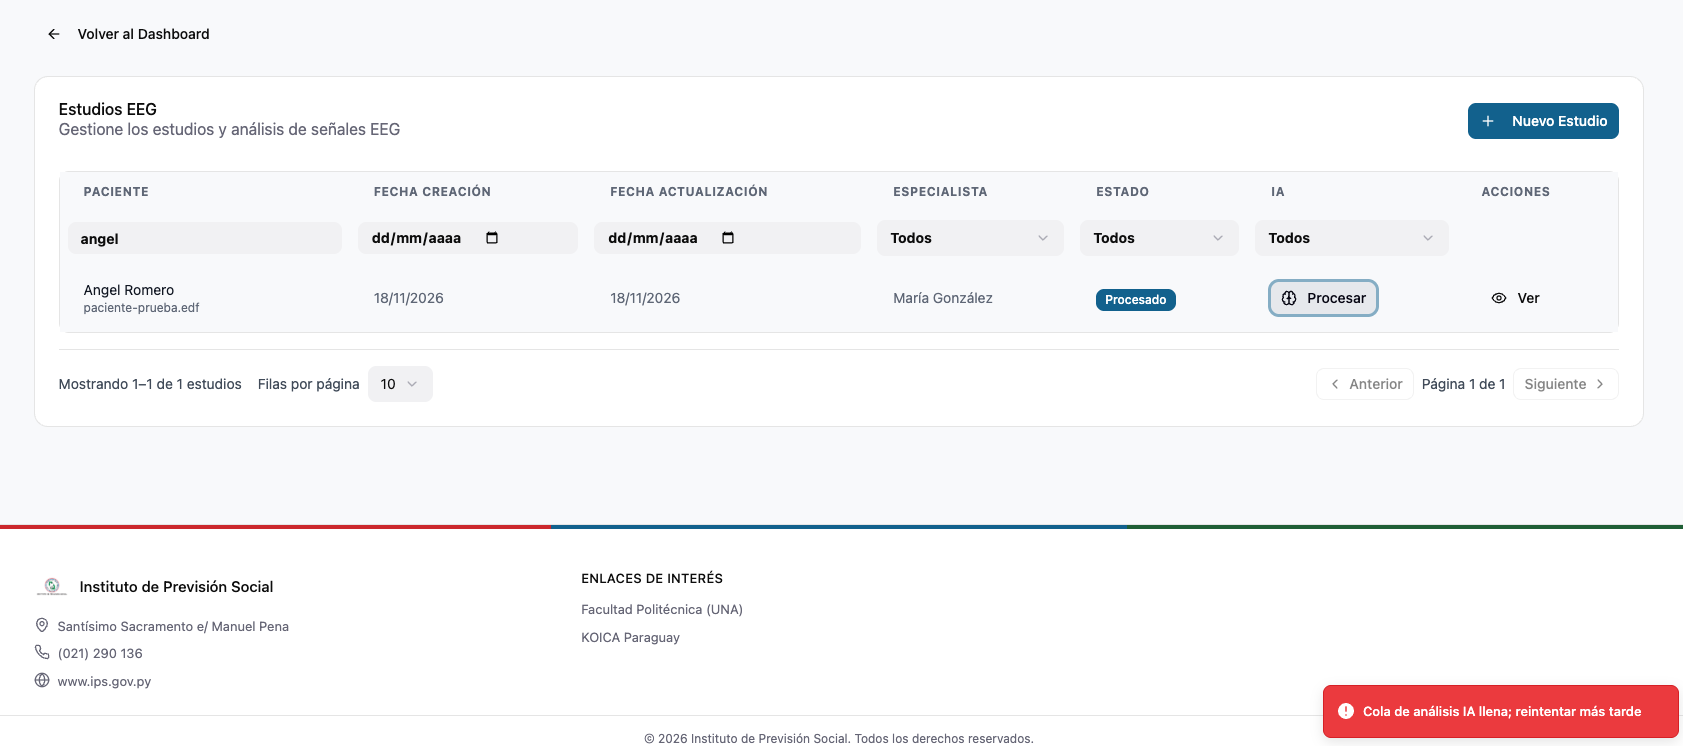
\includegraphics[width=0.90\textwidth]{Chapter6/Chapter6Figs/PI16_mensaje_cola_llena.png}
    \caption{Mensaje presentado al solicitar un análisis con la cola de procesamiento llena.}
    \label{fig:pi16-mensaje-cola-llena}
\end{figure}

Finalmente, se inició nuevamente el motor de procesamiento.
El motor tomó el primer trabajo y, 4 segundos después de liberarse ese lugar en la cola, el encolado automático registró la ejecución del tercer estudio, sin intervención del usuario.
Los tres análisis se ejecutaron de forma sucesiva y finalizaron correctamente.
Al concluir, cada estudio contaba con un único registro de ejecución y no quedaban trabajos en cola ni en curso.
La Figura~\ref{fig:pi16-listado-tres-analizados} presenta los tres estudios con la indicación «IA listo».

\begin{figure}[htbp]
    \centering
    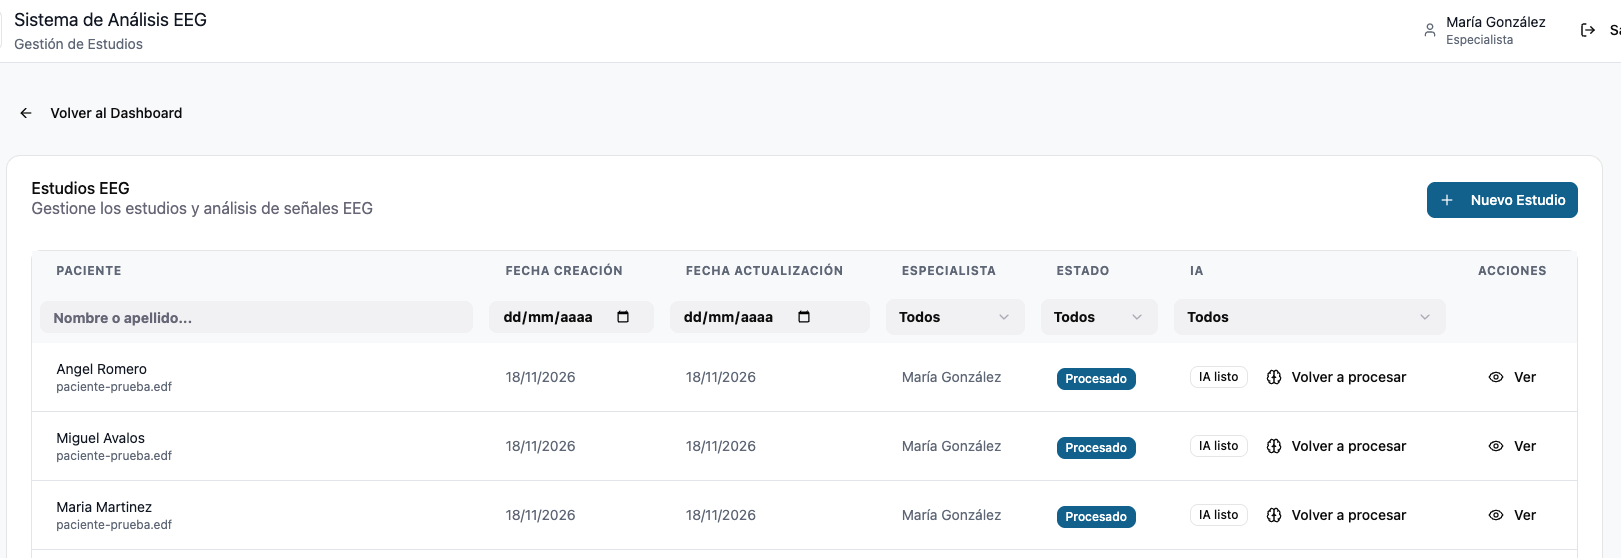
\includegraphics[width=0.90\textwidth]{Chapter6/Chapter6Figs/PI16_listado_tres_analizados.png}
    \caption{Los tres estudios con el análisis mediante IA finalizado.}
    \label{fig:pi16-listado-tres-analizados}
\end{figure}

Los resultados observados coincidieron con el comportamiento esperado para el caso PI-16, por lo que la prueba se clasificó como aprobada.
Con la cola llena, la solicitud adicional recibió un error controlado y coherente entre la API de inteligencia artificial y el \textit{backend}, ningún estudio se perdió ni quedó con una ejecución en estado de error, y el estudio rechazado se procesó de forma automática cuando hubo lugar disponible.

\subsubsection{Resultados de las pruebas de integración restantes}

Las pruebas de integración PI-06 a PI-17 fueron definidas
para evaluar la comunicación entre los componentes
responsables del procesamiento mediante inteligencia
artificial, la persistencia de resultados, la sincronización
de información y la gestión de situaciones excepcionales.

Para facilitar la presentación de los resultados, estos
casos se agrupan según las funcionalidades y los
componentes involucrados.

\begin{table}[htbp]
\centering
\caption{Resumen de las pruebas de integración PI-06 a PI-17.}
\label{tab:resumen_pruebas_integracion}
\small
\begin{tabular}{|p{1.5cm}|p{4cm}|p{6cm}|}
\hline
\textbf{Pruebas} &
\centering\arraybackslash\textbf{Funcionalidad evaluada} &
\textbf{Estado de verificación} \\ \hline

PI-06 a PI-08 &
Ejecución del procesamiento mediante IA,
persistencia y consulta de resultados. &
Aprobadas. Las solicitudes generaron ejecuciones identificables, sin duplicados, y el motor tomó los trabajos pendientes. \\ \hline

PI-09 a PI-12 &
Seguimiento del procesamiento, propagación de
estados, recuperación de resultados y programación
automática. &
Aprobadas. Se verificó la actualización de actividad del motor, la propagación de estados hasta la interfaz, la recuperación de resultados y el inicio automático de ejecuciones. \\ \hline

PI-13 a PI-14 &
Generación de espectrogramas y registro
de eventos asociados a la IA. &
Aprobadas. Se obtuvieron los datos de los espectrogramas y se registraron los eventos del ciclo de ejecución. \\ \hline

PI-15 a PI-16 &
Gestión de indisponibilidad del servicio
y saturación de la cola de procesamiento. &
Aprobadas. Las condiciones excepcionales produjeron respuestas controladas, sin pérdida del estado de las ejecuciones. Su ejecución se documenta en las subsecciones correspondientes a PI-15 y PI-16. \\ \hline

PI-17 &
Sincronización de anotaciones médicas. &
Aprobada. Las anotaciones manuales y las ventanas confirmadas se registraron en el subsistema de IA. \\ \hline

\end{tabular}
\end{table}

Durante las verificaciones se confirmó la disponibilidad del servicio FastAPI, la comunicación entre contenedores y el funcionamiento de las tablas que gestionan las ejecuciones de IA.
El ciclo completo de procesamiento se ejecutó sobre estudios EEG reales, tal como se detalla en la sección de pruebas de integración con el servicio de IA.
En consecuencia, los casos PI-06 a PI-17 se consideran aprobados.


\subsection{Síntesis de los resultados}


Las pruebas de integración permitieron verificar el funcionamiento de los mecanismos de autenticación y autorización, así como la comunicación entre la interfaz web, el servidor de aplicaciones y la base de datos principal.

Asimismo, se comprobó la persistencia de la información de pacientes y estudios electroencefalográficos, incluyendo el almacenamiento de archivos EEG y su posterior recuperación para la visualización de las señales.

En relación con el subsistema de inteligencia artificial, las verificaciones realizadas permitieron comprobar la disponibilidad del servicio FastAPI, la preparación de la base de datos especializada y el ciclo integral de procesamiento, desde la solicitud de análisis hasta la generación y recuperación de nuevos resultados.

En consecuencia, las evidencias obtenidas permiten considerar satisfactorias las integraciones entre los componentes de EpilexIA, incluida la integración completa del subsistema de inteligencia artificial.


\section{Pruebas de integración con el servicio de IA}

Las pruebas de integración con el servicio de
inteligencia artificial tuvieron como propósito
evaluar la comunicación entre el servidor de
aplicaciones de EpilexIA, la API desarrollada
con FastAPI, el motor de procesamiento y la
base de datos especializada en ejecuciones de IA.

Las verificaciones se realizaron en el entorno desplegado de EpilexIA, con los servicios ejecutándose en contenedores Docker.
Se comprobó la disponibilidad del servicio FastAPI mediante solicitudes HTTP, la preparación de las estructuras de persistencia en PostgreSQL y la comunicación entre los servicios.

Sobre este entorno se ejecutó el ciclo completo de procesamiento con seis estudios EEG reales de pacientes del Hospital Central del IPS, cargados en formato EDF tal como los exporta el equipo de adquisición.
Para cada estudio se solicitó el análisis desde la interfaz web y se observó la asignación de un identificador de ejecución, la toma del trabajo por parte del motor, la propagación de los estados hasta la interfaz y, una vez finalizado el procesamiento, la recuperación y presentación de los intervalos identificados en el visualizador EEG.
En los seis casos la ejecución finalizó correctamente.

Todas las ejecuciones se realizaron con el modelo HGB~2.0, descrito en la Sección~\ref{subsec:modelo-vigente-hgb}.
Los resultados fueron revisados por la médica especialista en epileptología, quien clasificó cada intervalo señalado por el modelo y agregó una descripción cuando lo consideró pertinente.
A modo de ejemplo, en uno de los estudios el modelo señaló once intervalos: la especialista confirmó diez como anomalías, identificó el restante como un artefacto de movimiento y registró manualmente una anomalía adicional.
La Figura~\ref{fig:ia-revision-listado} muestra el panel de anomalías de dicho estudio, con las etiquetas y descripciones incorporadas por la especialista, y la Figura~\ref{fig:ia-revision-manual} presenta la anomalía registrada manualmente.

\begin{figure}[H]
    \centering
    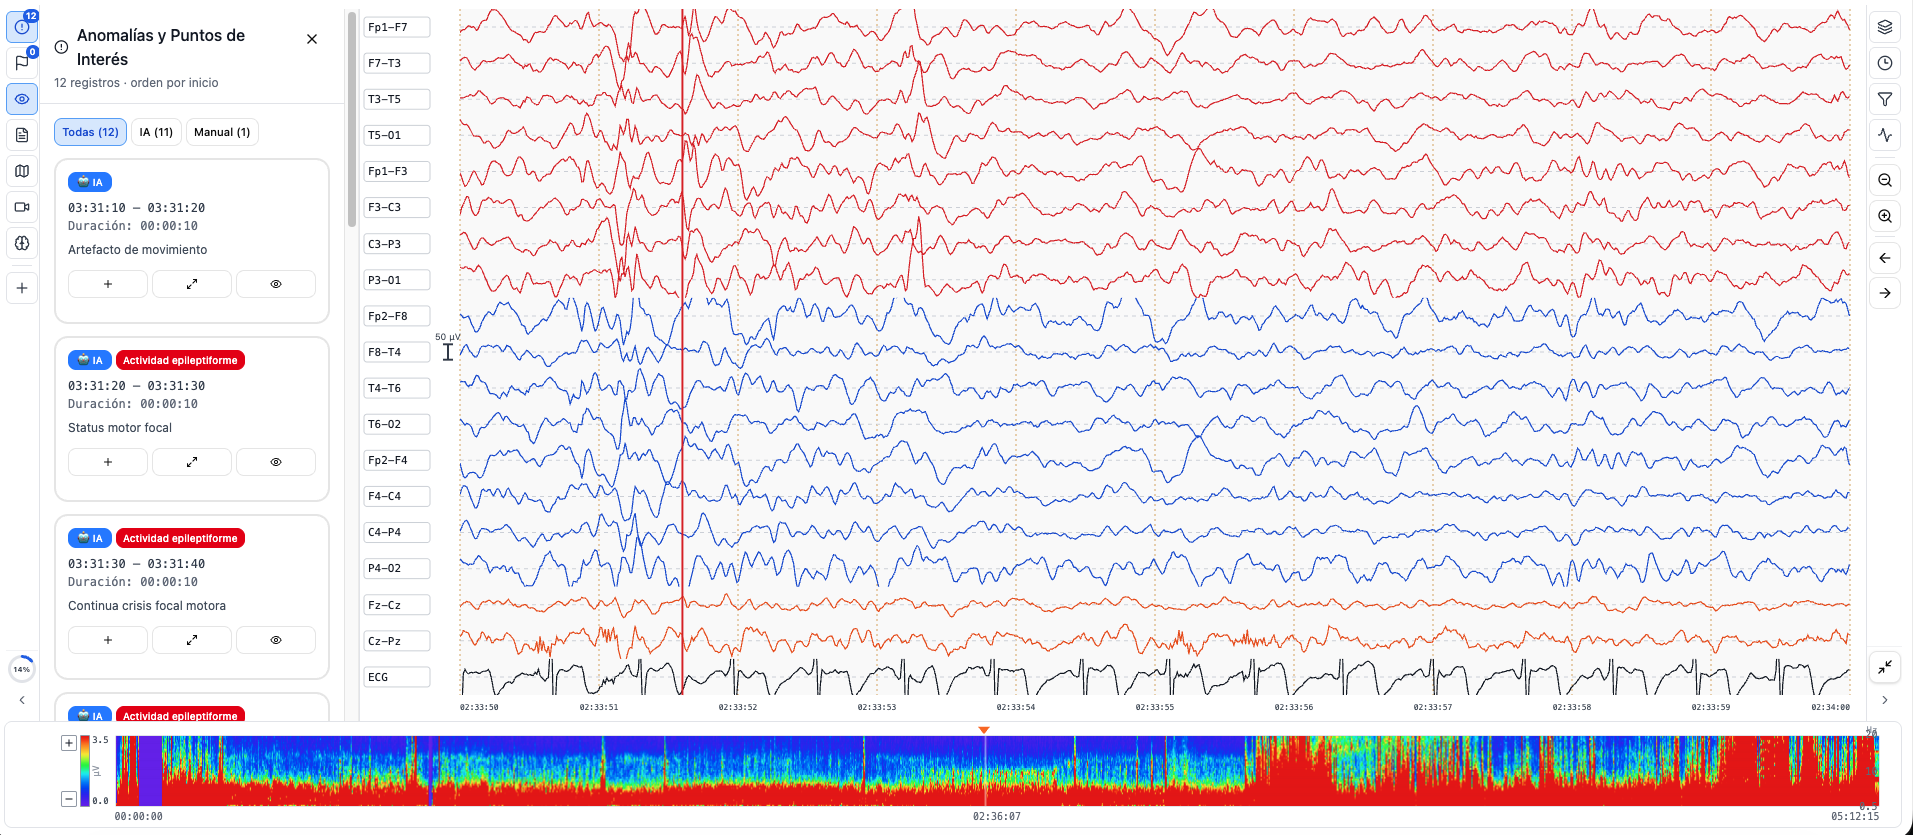
\includegraphics[width=0.95\textwidth]{Chapter6/Chapter6Figs/ia_revision_listado.png}
    \caption{Intervalos identificados por el modelo HGB~2.0 en un estudio real, clasificados y descritos por la especialista en EpilexIA.}
    \label{fig:ia-revision-listado}
\end{figure}

\begin{figure}[H]
    \centering
    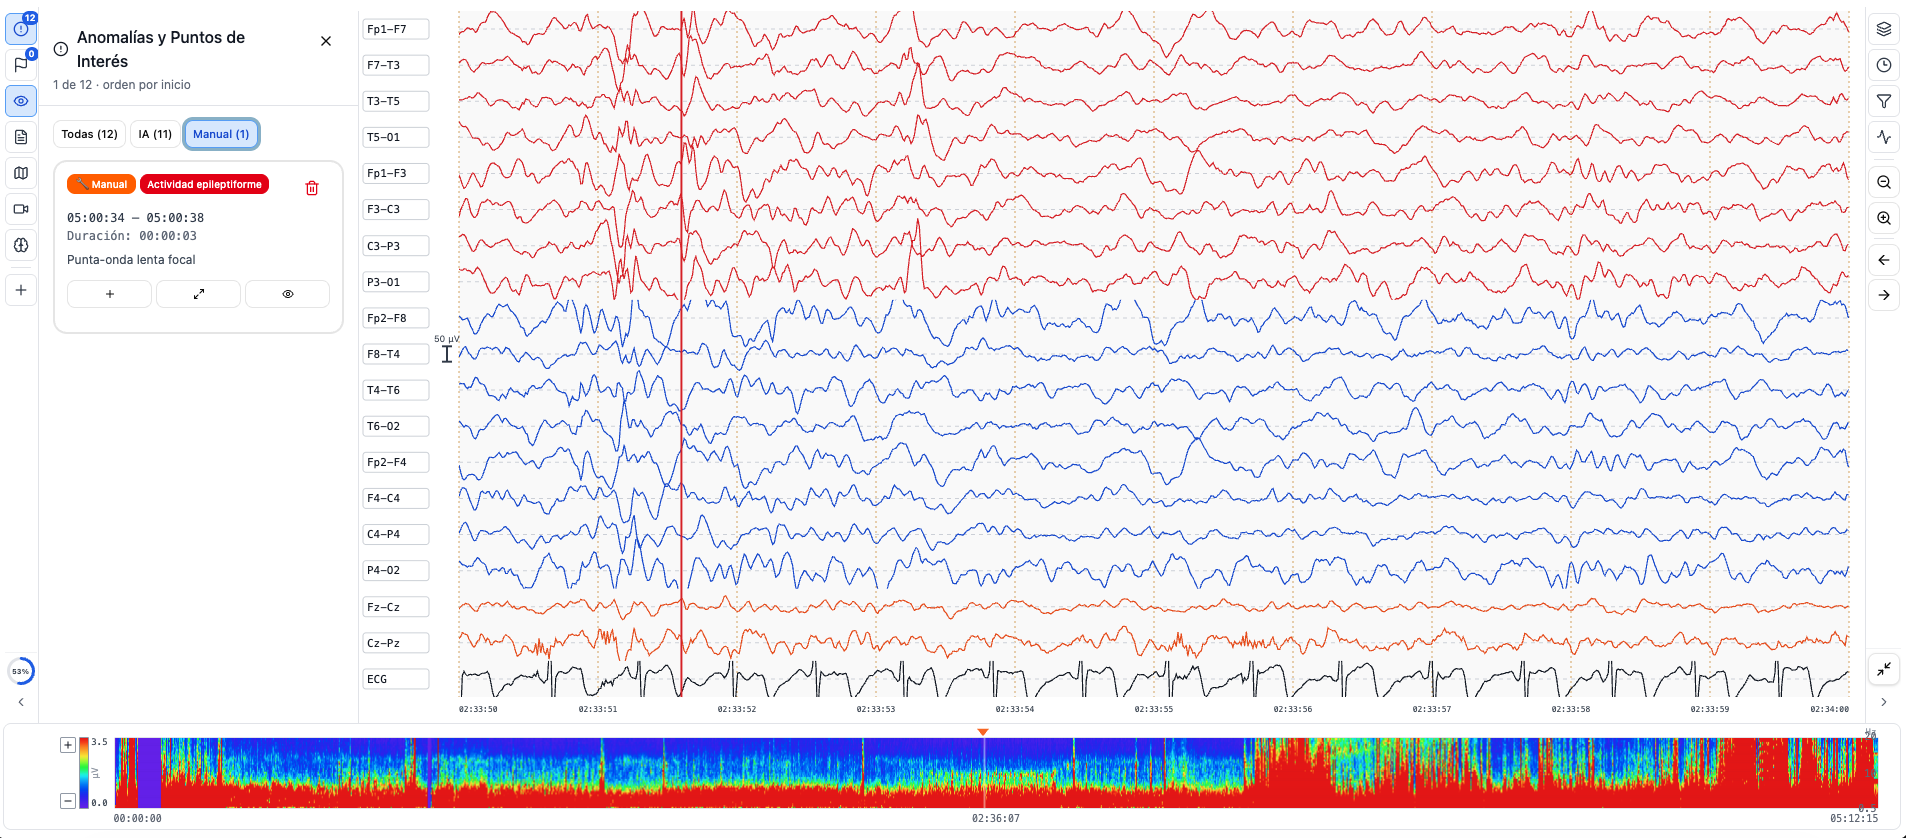
\includegraphics[width=0.95\textwidth]{Chapter6/Chapter6Figs/ia_revision_manual.png}
    \caption{Anomalía registrada manualmente por la especialista en el mismo estudio, como complemento de los resultados del modelo.}
    \label{fig:ia-revision-manual}
\end{figure}


Por consiguiente, las pruebas realizadas permitieron verificar la integración completa entre los componentes del subsistema de IA, desde la solicitud de análisis hasta la presentación de resultados en la interfaz web.
Estas verificaciones corresponden al funcionamiento integrado del sistema sobre un conjunto reducido de estudios y no constituyen una evaluación estadística del desempeño diagnóstico del modelo.


Cabe señalar que la prueba funcional PF-10, descrita anteriormente, se realizó utilizando resultados de inteligencia artificial que ya se encontraban almacenados en la base de datos, por lo que su alcance se limita a la consulta y visualización de dichos registros. La ejecución completa del motor de IA se verificó de manera independiente mediante las pruebas descritas en esta sección.


\section{Evaluación de usabilidad}


La evaluación de usabilidad de EpilexIA incluyó sesiones de prueba con una médica especialista en epileptología del Instituto de Previsión Social (IPS), perteneciente al grupo de usuarios destinatarios de la plataforma. El propósito fue observar la interacción de la profesional con las funcionalidades relacionadas con su actividad clínica.

Durante las sesiones, la especialista realizó tareas representativas del flujo de trabajo previsto, entre ellas la carga de archivos EEG en formato EDF, la exploración de señales electroencefalográficas mediante el visualizador, el marcado manual de posibles anomalías y la elaboración del informe médico correspondiente.

Estas actividades permitieron observar la utilización directa de las herramientas disponibles y comprobar que la profesional pudo completar las tareas descritas en el escenario evaluado.

La evaluación tuvo carácter exploratorio y cualitativo. No se aplicaron cuestionarios estandarizados de usabilidad ni se realizaron mediciones sistemáticas de tiempos de ejecución, tasas de error o satisfacción de la usuaria. Por consiguiente, los resultados no permiten establecer indicadores cuantitativos de eficacia, eficiencia o satisfacción.

La realización de evaluaciones adicionales con un mayor número de profesionales y procedimientos sistemáticos de medición permitiría obtener resultados más representativos sobre la experiencia de uso de EpilexIA.


\section{Validación en el contexto del Hospital Central del IPS}


Como parte de las actividades de validación contextual de EpilexIA, se realizaron sesiones de prueba en el consultorio de una médica especialista en epileptología, ubicado en el Hospital Central del Instituto de Previsión Social (IPS).

Las sesiones se desarrollaron durante los meses de septiembre y octubre de 2026, mediante visitas semanales realizadas los días jueves, de 10:00 a 13:00, con la participación del equipo de desarrollo.
En ellas, la especialista cargó y revisó en la plataforma seis estudios EEG de pacientes del hospital, exportados en formato EDF desde el equipo de adquisición.

La profesional accedió a la plataforma, desplegada en la nube, tanto desde su propia computadora portátil, con el navegador Google Chrome, como desde los equipos del hospital, utilizando en ambos casos sus credenciales de usuario.
En el primer caso empleó su propia conexión a internet y, en el segundo, la red del hospital, lo que permitió observar el comportamiento del sistema con distintos dispositivos y condiciones de conectividad.
Los estudios cargados fueron exportados por la especialista desde el equipo de adquisición del servicio.

Durante las sesiones se desarrolló un flujo de trabajo relacionado con el análisis de estudios electroencefalográficos, cuyas actividades se describieron en la sección anterior. La experiencia proporcionó evidencia inicial de utilización de la plataforma en el contexto institucional para el cual fue concebida.

Durante las sesiones, la especialista formuló observaciones sobre el funcionamiento de la plataforma, que el equipo de desarrollo registró e incorporó de manera progresiva entre una visita y la siguiente.
El Cuadro~\ref{tab:observaciones-especialista} resume dichas observaciones, clasificadas en ajustes de experiencia de uso, corrección de errores y optimizaciones generales del sistema.
Las versiones del sistema descritas en los capítulos anteriores ya incorporan las mejoras implementadas.

\begingroup
\small
\begin{longtable}{|p{0.8cm}|p{9.6cm}|p{2.6cm}|}
\caption{Observaciones surgidas en las sesiones de validación con la especialista y estado de su incorporación.}
\label{tab:observaciones-especialista}\\
\hline
\textbf{N.º} & \textbf{Observación o mejora} & \textbf{Estado} \\
\hline
\endfirsthead

\multicolumn{3}{c}{\textit{Continuación del Cuadro~\thetable}}\\
\hline
\textbf{N.º} & \textbf{Observación o mejora} & \textbf{Estado} \\
\hline
\endhead

\multicolumn{3}{|l|}{\textbf{Ajustes de experiencia de uso}} \\
\hline
1 & Sensibilidad predeterminada de 50~$\mu$V para el canal de ECG. & Implementada \\
\hline
2 & Configuración de filtros independiente para cada canal. & Implementada \\
\hline
3 & Exclusión del canal de ECG de los filtros globales. & Implementada \\
\hline
4 & Incorporación de las derivaciones de línea media del sistema 10-20. & Implementada \\
\hline
5 & Posibilidad de desactivar un canal ante electrodos defectuosos. & Implementada \\
\hline
6 & Colores diferenciados por grupo de derivaciones y para el ECG, de forma análoga al equipo de adquisición. & Implementada \\
\hline
7 & Navegación continua del trazado mediante el teclado y el ratón. & Implementada \\
\hline
8 & Visualización del trazado completo en una única ventana, sin desplazamiento vertical. & Implementada \\
\hline
9 & Espectrograma con referencias temporales para la navegación. & Implementada \\
\hline
10 & Marcado manual de intervalos que se extienden más allá de la ventana visible. & Implementada \\
\hline
11 & Disponibilidad del video en el modo de pantalla completa. & Implementada \\
\hline
12 & Pausa y reanudación del video mediante la barra espaciadora. & Implementada \\
\hline
13 & Ventanas flotantes de tamaño ajustable para el video y el mapa de electrodos. & Implementada \\
\hline
14 & Registro automático en el informe de las anomalías incorporadas, manuales o identificadas mediante IA. & Implementada \\
\hline
15 & Consulta del informe en un panel lateral del modo de pantalla completa. & Implementada \\
\hline
16 & Ejecución del análisis de IA desde el modo de pantalla completa. & Implementada \\
\hline
17 & Avance por ventana con las flechas del teclado y avance continuo por segundo mediante el ratón. & Implementada \\
\hline
18 & Ajuste de la sensibilidad con las flechas del teclado. & Implementada \\
\hline
19 & Sincronización del video al navegar hacia un punto de interés. & Implementada \\
\hline
20 & Ampliación de las etiquetas disponibles para clasificar anomalías. & Pendiente \\
\hline
\multicolumn{3}{|l|}{\textbf{Corrección de errores}} \\
\hline
21 & Corrección de la frecuencia del filtro \textit{Notch} a 50~Hz. & Implementada \\
\hline
22 & Recorte de los trazados al área de su canal, para evitar la superposición con canales adyacentes. & Implementada \\
\hline
23 & Corrección del ordenamiento del listado de anomalías. & Implementada \\
\hline
24 & Unificación del formato de hora (HH:MM:SS). & Implementada \\
\hline
25 & Revisión de la amplitud del canal de ECG con sensibilidad de 50~$\mu$V. & Pendiente \\
\hline
\multicolumn{3}{|l|}{\textbf{Optimizaciones generales del sistema}} \\
\hline
26 & Envío de las anomalías manuales al subsistema de IA para la retroalimentación de los modelos. & Implementada \\
\hline
27 & Optimización del consumo de recursos durante la ejecución del análisis de IA. & Implementada \\
\hline
28 & Procesamiento en paralelo del análisis de IA para estudios pendientes de ejecución. & Implementada \\
\hline
29 & Inicio del análisis de IA una vez finalizadas la carga del estudio y la conversión del video, para evitar la competencia por recursos del servidor. & Implementada \\
\hline
\end{longtable}
\endgroup

No obstante, estas actividades se realizaron con una especialista y no constituyeron una validación clínica integral ni una evaluación estadística del desempeño diagnóstico. La revisión de los resultados del subsistema de inteligencia artificial se efectuó sobre un conjunto reducido de estudios.

En consecuencia, las sesiones aportaron evidencia sobre la utilización de EpilexIA en el entorno hospitalario del IPS. Para determinar su aplicabilidad clínica de manera más amplia, serían necesarias evaluaciones adicionales con otros profesionales y una mayor diversidad de estudios EEG.

Como parte de la preparación para el uso del sistema en el hospital, se elaboraron y entregaron tres documentos: un manual de usuario para los perfiles Especialista y Técnico, un manual para el equipo de TI responsable de la administración del sistema y una guía específica para la exportación y carga de estudios, que es la tarea central del personal técnico.


\section{Síntesis de la evaluación por aspectos de calidad}
\label{sec:sintesis-aspectos}

El Cuadro~\ref{tab:sintesis-aspectos} sintetiza, para cada aspecto de calidad considerado, los puntos cubiertos por las pruebas de este capítulo y por las pruebas automatizadas de los repositorios, y los que no fueron cubiertos.
La organización de la evaluación y de su reporte toma como referencia las guías GEP-HI \citep{Nykanen2011GEPHI} y STARE-HI \citep{Talmon2009STAREHI}.
Las guías y normas citadas se emplean como marco de referencia; el presente trabajo no afirma conformidad ni certificación respecto de ninguna de ellas.

\begingroup
\footnotesize
\setlength{\tabcolsep}{4pt}
\renewcommand{\arraystretch}{1.15}
\begin{longtable}{|>{\raggedright\arraybackslash}p{0.19\textwidth}|>{\raggedright\arraybackslash}p{0.46\textwidth}|>{\raggedright\arraybackslash}p{0.25\textwidth}|}
\caption{Síntesis de la evaluación de EpilexIA por aspectos de calidad.}
\label{tab:sintesis-aspectos}\\
\hline
\textbf{Aspecto y referencia} & \textbf{Puntos cubiertos y pruebas realizadas} & \textbf{Puntos no cubiertos} \\
\hline
\endfirsthead

\multicolumn{3}{c}{\textit{Continuación del Cuadro~\thetable}}\\
\hline
\textbf{Aspecto y referencia} & \textbf{Puntos cubiertos y pruebas realizadas} & \textbf{Puntos no cubiertos} \\
\hline
\endhead

\textbf{Diseño y reporte de la evaluación} \citep{Nykanen2011GEPHI,Talmon2009STAREHI} &
Definición de la estrategia y de los ámbitos de prueba; casos con procedimiento, resultado esperado y resultado obtenido; descripción del contexto, del sistema y de los participantes; declaración de limitaciones. &
Plan formal de evaluación previo a la ejecución; gestión de riesgos del estudio; reporte de la totalidad de los elementos de STARE-HI. \\
\hline

\textbf{Usabilidad} \citep{ISO9241-11:2018,Brooke1996SUS} &
Observación cualitativa, sin medición de indicadores: la especialista completó las tareas del flujo clínico en sesiones semanales durante dos meses. Contexto de uso real: equipos y red del hospital. Observaciones registradas e incorporadas (Cuadro~\ref{tab:observaciones-especialista}). Documentación entregada: manual de usuario para especialistas y técnicos, manual para el equipo de TI a cargo de la administración del sistema y guía específica de carga de estudios. &
Medición de eficacia y eficiencia (tareas completadas, tiempos y errores); satisfacción mediante el cuestionario SUS; más de un participante; perfiles Técnico y Administrador. \\
\hline

\textbf{Rendimiento} &
Sin evaluación. &
Trabajo futuro. \\
\hline

\textbf{Fiabilidad} &
Seguimiento de la actividad del motor (PI-09); comportamiento ante la indisponibilidad del servicio de IA y ante la saturación de la cola, verificado en un entorno de pruebas local (PI-15, PI-16); persistencia de la información tras cerrar y reiniciar la sesión (PF-09, PF-11, PF-13); pruebas automatizadas de los reintentos en la carga de archivos. &
Ensayos de fallos provocados durante el procesamiento. \\
\hline

\textbf{Seguridad y control de acceso} \citep{OWASP2025ASVS} &
Autenticación (PF-01, PF-02, PI-01); gestión y revocación de sesiones (PI-03); autorización por rol y por recurso, verificada también en el \textit{backend} (PF-12, PF-14, PI-02) y mediante pruebas automatizadas; registro de auditoría (PF-15, PI-14). Mecanismos de protección de datos implementados: contraseñas almacenadas mediante \textit{hash}, \textit{tokens} con vencimiento para sesiones y cuentas, enlaces para compartir estudios revocables, enmascarado de datos sensibles en los registros de ejecución, restricciones en la carga de archivos, componentes internos sin exposición a internet y comunicación mediante HTTPS. &
Verificación sistemática frente a los requisitos de la norma; pruebas de intrusión. \\
\hline

\textbf{Privacidad} &
Sin evaluación. &
Trabajo futuro. \\
\hline

\textbf{Fidelidad del visualizador} &
Sensibilidad (PF-06); montajes Doble Banana y Transversal (PF-07); filtros de corte inferior, de corte superior y \textit{Notch} (PF-08); pruebas automatizadas de filtros, unidades, escalas, eje temporal y montajes. &
Comparación cuantitativa con señales de comportamiento conocido. \\
\hline

\textbf{Interoperabilidad} \citep{Kemp1992EDF,KempOlivan2003EDFPlus} &
Lectura de registros EDF y EDF+, con pruebas automatizadas del lector; carga y procesamiento de registros exportados por el equipo de adquisición (PF-05, PI-05); seis estudios reales; conversión del video del equipo de adquisición a MP4; exportación del informe a PDF. &
Importación de las anotaciones de EDF+; comparación con un lector independiente; intercambio con otros sistemas. \\
\hline

\textbf{Accesibilidad} \citep{W3C2023WCAG22} &
Sin evaluación. &
Trabajo futuro. \\
\hline

\textbf{Trazabilidad} &
Auditoría de las acciones por usuario, con consulta y filtros (PF-15); registro de eventos del ciclo de IA (PI-14); identificador, estado y parámetros de cada ejecución (PI-06, PI-10); vínculo entre resultados, ejecución e informe (PI-11, PI-17). &
Reconstrucción documentada de una ejecución completa, del registro EEG al informe. \\
\hline

\textbf{Verificación funcional integrada} &
15 casos funcionales (PF-01 a PF-15) y 17 de integración (PI-01 a PI-17) aprobados; flujo completo sobre seis estudios reales, del registro del estudio al informe; pruebas automatizadas en los repositorios. &
Pruebas automatizadas de extremo a extremo; integración continua; otros navegadores y tamaños de pantalla. \\
\hline

\end{longtable}
\endgroup

Tres aspectos no fueron evaluados y se plantean como trabajo futuro: el rendimiento, la privacidad y la accesibilidad.
Respecto de la privacidad, el subsistema de inteligencia artificial recibe el número de documento del paciente, que se utiliza para vincular los estudios y las ejecuciones entre ambas bases de datos.
Como trabajo futuro se prevé reemplazar el documento por un identificador único sin significado.


\clearpage
\section[Análisis del cumplimiento de los requerimientos]{Análisis del cumplimiento de los \\requerimientos}

El análisis del cumplimiento de los requerimientos
de EpilexIA se realizó considerando las
funcionalidades implementadas y las evidencias
obtenidas durante las pruebas funcionales,
de integración y de utilización del sistema.

Las verificaciones efectuadas permitieron
comprobar el funcionamiento de los mecanismos
de autenticación y autorización, la gestión
de pacientes y estudios electroencefalográficos,
así como el almacenamiento y la visualización
de señales EEG.

Adicionalmente, durante las sesiones de prueba
realizadas con una especialista en epileptología
del IPS, se verificó la utilización de las
funcionalidades de carga de archivos EDF,
marcado manual de posibles anomalías y
elaboración de informes médicos. Esta
experiencia aportó evidencia de uso de
funciones vinculadas directamente con el
trabajo clínico de los profesionales
destinatarios del sistema.


En cuanto al subsistema de inteligencia artificial, se comprobó la disponibilidad de los servicios, la preparación de las estructuras de persistencia y la ejecución integral del procesamiento mediante IA sobre estudios reales, desde la solicitud de análisis hasta la generación, recuperación y presentación de nuevos resultados.


En términos generales, las evidencias obtenidas permiten establecer un cumplimiento verificable de los requerimientos asociados a las funcionalidades de gestión, visualización y procesamiento mediante inteligencia artificial.

Este análisis se limita a los escenarios
efectivamente evaluados y no implica que
todos los requerimientos del sistema hayan
sido comprobados exhaustivamente.


\clearpage
\section[Análisis de los resultados respecto de los objetivos e hipótesis]{Análisis de los resultados respecto de los \\objetivos e hipótesis}

Los resultados obtenidos durante las pruebas
permitieron evaluar el grado de cumplimiento
de los objetivos planteados para el desarrollo
de EpilexIA, considerando tanto las
funcionalidades implementadas como las
verificaciones realizadas.

En relación con el objetivo de desarrollar
una plataforma web para apoyar el análisis
de estudios electroencefalográficos, se
comprobó el funcionamiento de las
funcionalidades de gestión de pacientes,
registro de estudios, almacenamiento y
visualización de señales EEG.

Asimismo, las sesiones de prueba realizadas
con una especialista en epileptología del
IPS permitieron observar la utilización de
herramientas relacionadas con el trabajo
clínico, incluyendo la carga de archivos
EDF, el marcado de posibles anomalías
y la elaboración de informes médicos.


Respecto a la incorporación de técnicas de inteligencia artificial, se verificó la integración de los servicios responsables de gestionar las solicitudes de procesamiento y la ejecución completa del modelo HGB~2.0 sobre estudios reales, con generación y presentación de nuevos resultados en la plataforma.


En consecuencia, los resultados respaldan el cumplimiento de los objetivos asociados al desarrollo e implementación de la plataforma y proporcionan evidencia de su utilización en el contexto hospitalario.
La hipótesis formulada en el capítulo introductorio del libro, según la cual un sistema web integrado puede contribuir a mejorar el flujo de trabajo relacionado con el análisis de estudios electroencefalográficos, se considera respaldada dentro del alcance de la evaluación realizada, sobre un conjunto reducido de estudios revisados por una especialista.
Su contrastación se desarrolla en el capítulo de conclusiones del libro.


\clearpage
\lhead{\emph{Referencias}}
\addtotoc{Referencias}
\bibliographystyle{apacite}
\bibliography{References/references}
\end{document}
